\documentclass[dvipdfm]{book}
\setlength{\textwidth}{400pt}

%%%%%%%%%%%%%%%%%%%%%%%%%%%%%%%%%%%%%%%%%%%%%%%%%%%%%%%%%%%%%%%%%%%%%%%%%%
%%% Axiom Literate Programming Chunk Support
%%%%%%%%%%%%%%%%%%%%%%%%%%%%%%%%%%%%%%%%%%%%%%%%%%%%%%%%%%%%%%%%%%%%%%%%%%
%% This defines the TeX support for Axiom.

%% Latex Chunk support
%% This is the chunk environment that replaces the use of web-like tools
%%
%% \begin{verbatim}
%% To use the command you would write
%%    \begin{chunk}{some random string}
%%    random code to be verbatim formatted
%%    \end{chunk}
%% 
%%  This version prints 
%%                     --- some random string ---
%%    random code to be verbatim formatted
%%                     --------------------------
%% \end{verbatim}

%%%%%%%%%%%%%%%%%%%%%%%%%%%%%%%%%%%%%%%%%%%%%%%%%%%%%%%%%%%%%%%%%%%%%%%%%%
%%% The verbatim package quotes everything within its grasp and is used to
%%% hide and quote the source code during latex formatting. The verbatim
%%% environment is built in but the package form lets us use it in our
%%% chunk environment and it lets us change the font.
%%%

\usepackage{verbatim}

%%%%%%%%%%%%%%%%%%%%%%%%%%%%%%%%%%%%%%%%%%%%%%%%%%%%%%%%%%%%%%%%%%%%%%%%%%
%%% 
%%% Make the verbatim font smaller
%%% Note that we have to temporarily change the '@' to be just a character
%%% because the \verbatim@font name uses it as a character
%%%

\chardef\atcode=\catcode`\@
\catcode`\@=11
\renewcommand{\verbatim@font}{\ttfamily\small}
\catcode`\@=\atcode

%%%%%%%%%%%%%%%%%%%%%%%%%%%%%%%%%%%%%%%%%%%%%%%%%%%%%%%%%%%%%%%%%%%%%%%%%%
%%% This declares a new environment named ``chunk'' which has one
%%% argument that is the name of the chunk. All code needs to live
%%% between the \begin{chunk}{name} and the \end{chunk}
%%% The ``name'' is used to define the chunk.
%%% Reuse of the same chunk name later concatenates the chunks

%%% For those of you who can't read latex this says:
%%% Make a new environment named chunk with one argument
%%% The first block is the code for the \begin{chunk}{name}
%%% The second block is the code for the \end{chunk}
%%% The % is the latex comment character

%%% We have two alternate markers, a lightweight one using dashes
%%% and a heavyweight one using the \begin and \end syntax
%%% You can choose either one by changing the comment char in column 1
 
\newenvironment{chunk}[1]{%   we need the chunkname as an argument
{\ }\newline\noindent%                    make sure we are in column 1
%{\small $\backslash{}$begin\{chunk\}\{{\bf #1}\}}% alternate begin mark
\hbox{\hskip 2.0cm}{\bf --- #1 ---}%      mark the beginning
\verbatim}%                               say exactly what we see
{\endverbatim%                            process \end{chunk}
\par{}%                                   we add a newline
\noindent{}%                              start in column 1
\hbox{\hskip 2.0cm}{\bf ----------}%      mark the end
%$\backslash{}$end\{chunk\}%              alternate end mark (commented)
\par%                                     and a newline
\normalsize\noindent}%                    and return to the document

%%%%%%%%%%%%%%%%%%%%%%%%%%%%%%%%%%%%%%%%%%%%%%%%%%%%%%%%%%%%%%%%%%%%%%%%%%
%%% This declares the place where we want to expand a chunk

\providecommand{\getchunk}[1]{%
\noindent%
{\small $\backslash{}$begin\{chunk\}\{{\bf #1}\}}}% mark the reference

%%%%%%%%%%%%%%% end the literate program chunking code %%%%%%%%%%%%%%%%%%%

\usepackage[toc,page]{appendix} % add the appendix and a toc entry
\usepackage{multicol}           % split into multiple cols
\usepackage{color}
\definecolor{mygrey}{gray}{0.80}
\usepackage{graphicx}           % for includegraphics
\usepackage{url}                % for format of URLs
\usepackage{enumerate}          % for letters on enumerate
\usepackage{makeidx}            % for constructing the index
\makeindex                      % flag that we construct an index
\usepackage{hyperref}           % for hyperlinking (use blue for links)
\hypersetup{colorlinks=true,linkcolor=blue,pdfborderstyle={/S/U/W 1},
citecolor=red}

\begin{document}
\begin{titlepage}
{\center{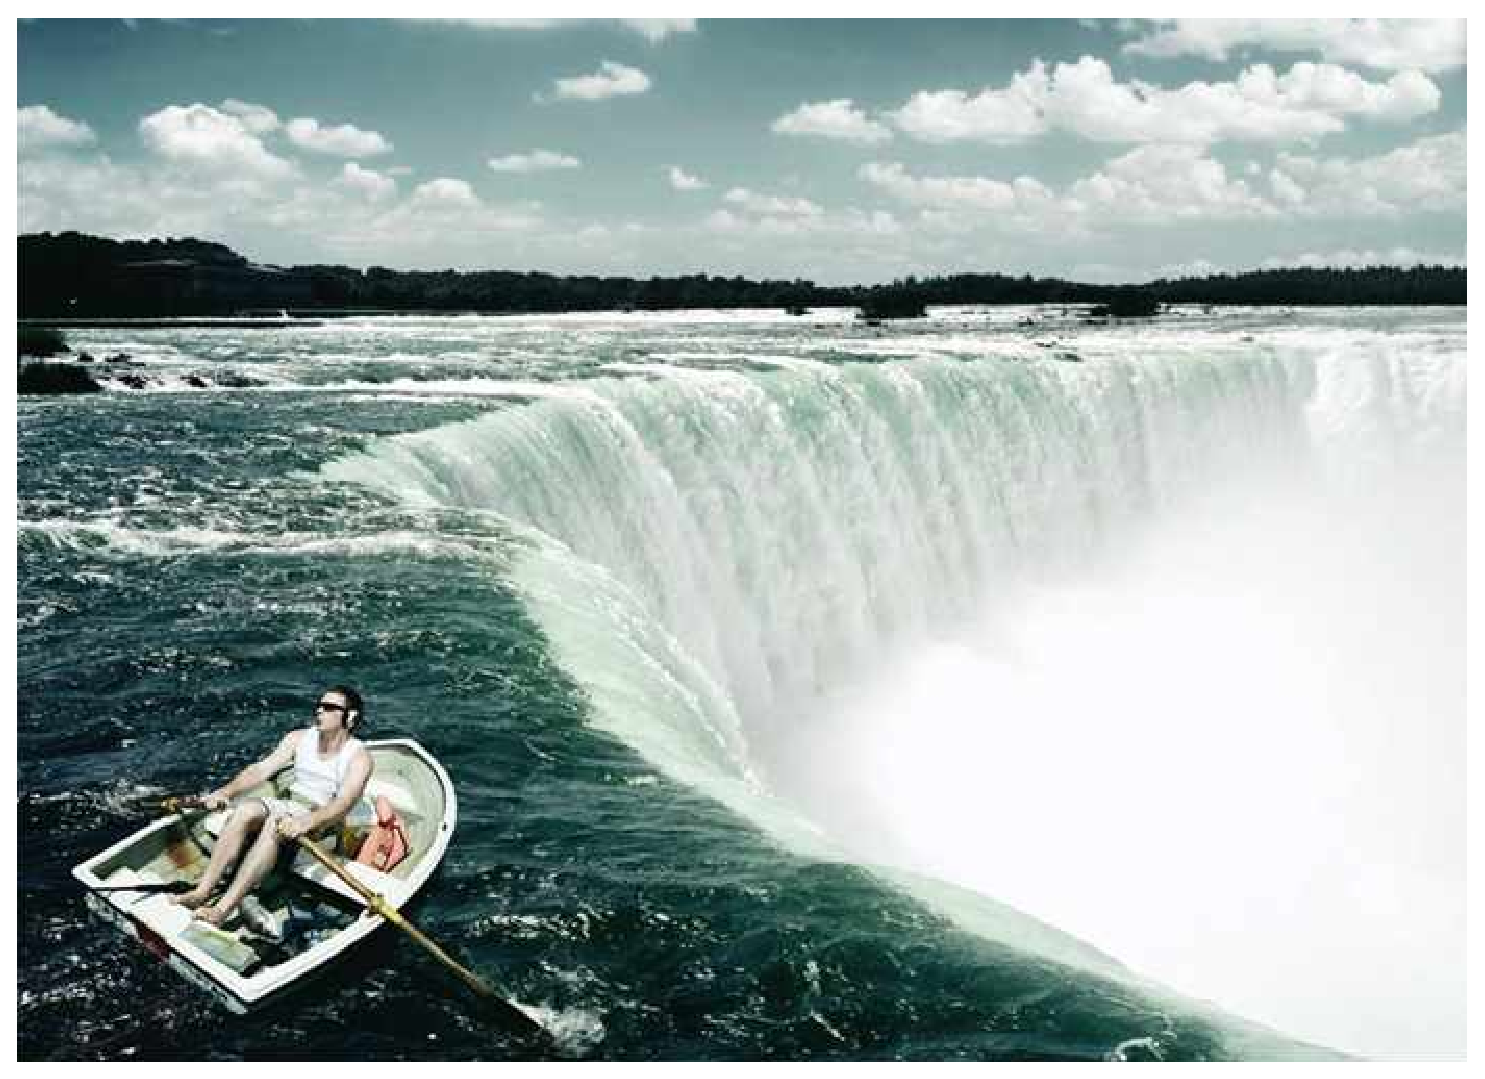
\includegraphics[scale=0.5]{eps/exfilt.eps}}}
\vskip 0.1in
\center{\huge{The EXFILT Project}}
\center{\large{Timothy Daly, Charles Howard, Ravi Starzl}}
\center{\large{Nanjie Chenglie, Hua Tang}}
\center{\huge{\today}}
\end{titlepage}
\begin{quote}
I believe that the time is ripe for significantly better documentation
of programs, and that we can best achieve this by considering programs
to be works of literature. Hence, my title ``Literate Programming''.

Let us change our traditional attitude to the construction of programs:
Instead of imagining that our main task is to instruct a computer what to do,
let us concentrate rather on explaining to human beings what we want a
computer to do.

{\bf -- Donald Knuth} \cite{50}
\end{quote}

This is a literate program. It is oriented toward communicating with
people and, as a side-effect, communicating with the machine. All of
the programs, data, and tests are included and are extracted from
this document to build the system. 

\tableofcontents
\chapter{Preface}
Exfiltration of confidential data is a growing concern as collections
of confidential information grow larger, these become high-value
targets. One recent example is the loss of 4.2 million records
containing the background checks for top secret security clearance
were exfiltrated from the Office of Personnel Management.

There are several layers of defense that could have, and should have,
been applied to this data. Apparently there was no mechanism to
recognize that this data was being stolen. At minimum, there ought to
be a last line of defense alert system.

A last line of defense would at least make people aware that 
confidential data was being copied. It should monitor the network
for confidential data transfer and, if any is found, raise an alarm.

The idea behind the current work is to prototype such a last line of
defense. We consider marking confidential documents held in storage
and examining data streams to detect that a confidential document is
being exfiltrated.

In this simple prototype we make several simplifying assumptions.

First, we assume that the data is marked by computing a SHA1 hash.
This hash can be kept in a network device table. The network device
computes a hash of document traffic. If the traffic hash matches a
hash in the table then it is a confidential document and an alert is
issued. The ``marker'' can be anything but SHA1 is simple.

Second, we assume that our device is ``plug-and-play'' in that it can
be plugged into the network just prior to leaving the premise.  It
could be applied in an internal network if there is a secure perimeter
around the data.

Third, we assume that the data in transit is a copy of the data in
storage. That is, there is no encryption or obfuscation applied to the
data between reading from storage and arriving at our device.

Our prototype is originally implemented in C running on a PC in order
to examine issues. However, it is clear that such an implementation
cannot keep up with network traffic.

After completing the first prototype we moved on to a Field
Programmable Gate Array (FPGA) hardware implementation. This can
operate at network speeds. We have a VHDL hardware interface which
feeds a primitive VHDL CPU. The CPU is programmed in Forth, a stack
based language.

\section{Overview}

We set up dual laptops, one containing the confidential information
and one trying to exfiltrate it. We used Wireshark to get packet
traces. We wrote C code to extract the confidential ile on the wire
and recognize that it was confidential. This was the initial prototype
plan.

Once that prototype was done we moved to an FPGA implementation. The
implementation uses a VHDL J1 processor which can be programmed in
Forth. We are working to get the bytes off the wire, into memory, 
and checking (using SHA1 in Forth) that we have the confidential file.
This is a hardware implementation of the prototype.



\chapter{EXFILT Plan Steps}
EXFILT will begin as a software-based set of technologies to prevent
sensitive information from traveling outside of a computer network.
The intent of the initial version is to create Intellectual Property
and a prototypical Proof of Concept to be used for fundraising.  As
such, hardware/firmware based implementations involving FPGA’s,
microprocessors and other embedded logic controllers are out of scope;
but might be developed at a later date.  Extensibility and
interoperability with potential future non-software based
implementations are not of major concern when building the initial
prototype version.

\vspace{2mm}
\noindent
{\bf Version 0.0}

The goal for this iteration is to construct a SNORT plugin (in C) for
use with Wireshark.  The plugin will use deep packet inspection to
detect a transfer of sensitive information by looking for the presence
of a SHA1 hash.  To allow us to focus on the complexities of getting a
basic plugin functioning, the only protocol and transfer type
addressed by this version will be an FTP Copy operation; and test data
will simply be unencrypted plain-text files.  Other formats and modes
like .docx and .pdf files, or email attachments will be addressed in
later iterations.

When the plugin detects sensitive information it will log the
date/time, origin IP, destination IP, and other details depending on
availability and usefulness.  At this stage it will not attempt to
terminate or block the transmission of data.

\vspace{2mm}
\noindent
{\bf Version 0.1}

This iteration involves the construction of a proxy server-like buffer
(in Java) for accumulating the entire set of packets in a
transmission, for subsequent inspection of file attributes (such as
file type), and syntactic analysis against a cohesive file.  The
buffering system at this point does not need to implement any
filtering/detection methods.  It simply needs to be able to accumulate
the packets in a transmission, then either stop the transmission by
sending it forward, or forward the transmission on to its final
destination.

\vspace{2mm}
\noindent
{\bf Version 0.2}

This iteration of the prototype will include one or more of the
following, depending on priorities, time, resources and discoveries as
they stand at the completion of Version 0.1:

\begin{enumerate}[A.]
\item An interface for end users to define syntactic filters (words,
phrases and patterns) to be used for detecting sensitive information
in transmissions accumulated in the Buffering system built in v0.1

\item Automated redaction of sensitive information through replacement of
detected sensitive information patterns with innocuous text prior to
re-transmission to the final destination

\item Support for file formats other than plain text (e.g.: .docx, .pdf,
.xls, etc…) Open source, Java-based readers for various file formats
might be used for this effort.  Since the goal of Version 0 is a
functional Proof Of Concept, proprietary document readers with lower
latency can be built in later development efforts.

\item Support for filtering email attachments, as well as communication
protocols other than FTP.  This effort could encompass changes to both
the Buffering and Filtering system and the SNORT plugin built in
version 0.0.
\end{enumerate}


\chapter{Threats and Risks}
\section{Threats}
\begin{itemize}
\item loss of customer data
\item loss of corporate data
\item theft of capital equipment
\item business disruption
\item reduced productivity
\item increased expense
\item regulatory violation
\item loss of public trust
\item stock loss
\end{itemize}

Risk = probability x cost

\subsection{Insider Threats}

ISO 17799 Code of Practice or Information Security Management
Internal Controls
  (COSO) Committee of Sponsoring Organizations of the Treadway Commission
  (CobiT) Control Objective for Information and related Technology

Operational Security:

\url{http://securityaffairs.co/wordpress/37368/security/operational-securit-user-education.html}


\chapter{AI and Exfiltration}
\section{The Problem}
Exfiltration is rarely accidental and confidential information does
not move itself. The key question becomes ``How to identify the actor?''

We can take a bottom-up approach to the problem. This involves several
layers, some of which are traditional and some which are not yet in use.

At the network layer we need to have ``sensors'' which can detect the
movement of confidential data across the security boundary. Various
sensing techniques exist. Indeed, we are building a network sensor
prototype which will detect an exfiltration.

At the monitoring layer we need rules that specify what actions to take.
Rule-based systems, usually built on SNORT or Linux IPTables,
allow actions such as DROPing a packet. However, this layer of rules is
too close to the metal and cannot see exfiltration events over normal
traffic avenues like FTP or email.

At the alert level we need network logging, again usually using things
like IPTable LOG rules.

There are issues that arise at the logging layer and above. 
For any network size, logging is useless if the logs are not reviewed.
But, almost no matter the size of the network, the number of people
available to review the logs is not sufficient to act on each event.

A network attack can easly swamp a network log file so that it either
contains too many entries or simply runs out of storage.

Worse, even if every event was tracked, there needs to be someone who
can provide an overview of all the events to extract the common elements.
These common elements need to be ``backtracked'' to find the actor(s).

This ``analysis'' layer is usually missing from network security.
At best it occurs as a post-mortem after a network breach. But given
the volume of traffic locally or in a data center, the likelyhood of
finding an exfiltration pattern is small.

\section{An Artificial Intelligence Approach}
Traditional Artificial Intelligence (AI) techniques can be applied to this
problem. Large volumes of data containing small patterns of information
are the normal domain of these systems. 

Usually the ``sensors'' are human-like, such as cameras for ``eyes'',
microphones for ``ears'', and robot arms for ``actuators''. But that
does not have to be the case. In a network environment the ``sensing''
equipment are low-level hardware and SNORT/IPTables firewall rules.

The AI problem, given the logs and active alerts on the sensors, is to
find elfiltration events, correlate the events with patterns, and from
those patterns identify the likely actor(s).


\chapter{Background}
\begin{itemize}
\item {\bf Packet filtering}
\url{https://www.youtube.com/watch?v=XHlqIqPvKw8}
\item {\bf Wireshark tutorial}
\url{https://www.youtube.com/watch?v=Lu05owzpSb8}
\item {\bf Art of Packet Analysis}
\url{https://www.youtube.com/watch?v=Qd6uDg9OGxM}
\item {\bf TCP/IP Packet analysis tutorials}
\url{https://www.youtube.com/watch?v=jWJIGqW6PrY&list=PLD57FE11C7A09034F&index=1}
\end{itemize}

\section{Protocols Introduction}
The File Transfer Protocol (FTP) is a standard network protocol used
to transfer computer files from one host to another host over a
TCP-based network, such as the Internet.\cite{10} FTP is built on a
client-server architecture and uses separate control and data
connections between the client and the server. FTP users may
authenticate themselves using a clear-text sign-in protocol, normally
in the form of a username and password, but can connect anonymously if
the server is configured to allow it. For secure transmission that
protects the username and password, and encrypts the content, FTP is
often secured with SSL/TLS (FTPS). SSH File Transfer Protocol (SFTP)
is sometimes also used instead, but is technologically different.

FTP may run in active or passive mode, which determines how the data
connection is established.\cite{11} In both cases, the client creates a TCP
control connection from a random, usually an unprivileged, port N to
the FTP server command port 21. In active mode, the client starts
listening for incoming data connections from the server on port M. It
sends the FTP command PORT M to inform the server on which port it is
listening. By default, M=N. The server then initiates a data channel
to the client from its port 20, the FTP server data port. In
situations where the client is behind a firewall and unable to accept
incoming TCP connections, passive mode may be used. In this mode, the
client uses the control connection to send a PASV command to the
server and then receives a server IP address and server port number
from the server,\cite{11,12} which the client then uses to open a data
connection from an arbitrary client port to the server IP address and
server port number received.\cite{13} Both modes were updated in September
1998 to support IPv6. Further changes were introduced to the passive
mode at that time, updating it to extended passive mode.\cite{14}

The server responds over the control connection with three-digit
status codes in ASCII with an optional text message. For example "200"
(or "200 OK") means that the last command was successful. The numbers
represent the code for the response and the optional text represents a
human-readable explanation or request (e.g. <Need account for storing
file>).\cite{10} An ongoing transfer of file data over the data connection
can be aborted using an interrupt message sent over the control
connection.

\begin{itemize}
\item FTP (File Transfer Protocol)\\
\begin{itemize}
\item Introduction video:\\
\url{http://www.lynda.com/FTP-tutorials/What-FTP/189068/364891-4.html}
\item Standard RFC (Request for Comments): 
\begin{itemize}
\item FTP Security Extensions: RFC 2228\\
\url{http://www.rfc-editor.org/rfc/rfc2228.txt}\\
\item Internationalization of the File Transfer Protocol: RFC 2640\\
\url{http://www.rfc-editor.org/rfc/rfc2640.txt}\\
\item Encryption using KEA and SKIPJACK: RFC 2773\\
\url{http://www.rfc-editor.org/rfc/rfc2773.txt}\\
\item Extensions to FTP: RFC 3659\\
\url{http://www.rfc-editor.org/rfc/rfc3659.txt}\\
\item FTP Command and Extension Registry: RFC 5797\\
\url{http://www.rfc-editor.org/rfc/rfc5797.txt}\\
\item File Transfer Protocol HOST Command for Virtual Hosts: RFC 7151\\
\url{http://www.rfc-editor.org/rfc/rfc7151.txt}\\
\end{itemize}
\end{itemize}
\item ARP (Address Resolution Protocol)\\
\begin{itemize}
\item Introduction video:\\
\url{https://www.youtube.com/watch?v=2ydK33mPhTY}\\
\item Standard RFC (Request for Comments): 
\begin{itemize}
\item IANA Allocation Guidelines for the Address Resolution 
Protocol (ARP): RFC 5494
\url{http://www.rfc-editor.org/rfc/rfc5494.txt}
\item A Reverse Address Resolution Protocol: RFC 903\\
\url{http://www.rfc-editor.org/rfc/rfc903.txt}
\item Inverse Address Resolution Protocol: RFC 2390\\
\url{http://www.rfc-editor.org/rfc/rfc2390.txt}
\item Address Resolution Protocol (ARP) Mediation for IP 
Interworking of Layer 2 VPNs: RFC 6575\\
\url{http://www.rfc-editor.org/rfc/rfc6575.txt}
\item FTP Command and Extension Registry: RFC 5797\\
\url{http://www.rfc-editor.org/rfc/rfc5797.txt}
\item File Transfer Protocol HOST Command for Virtual Hosts: RFC 7151\\
\url{http://www.rfc-editor.org/rfc/rfc7151.txt}
\end{itemize}
\end{itemize}
\item HTTP (Hypertext Transfer Protocol)\\
\begin{itemize}
\item Introduction video:\\
\url{https://www.youtube.com/watch?v=uvSIR2RhdXk}
\item Standard RFC (Request for Comments): \\
\begin{itemize}
\item Character Set and Language Encoding for Hypertext Transfer Protocol 
(HTTP) Header Field Parameters: RFC 5987 \\
\url{http://www.rfc-editor.org/rfc/rfc5987.txt}
\item Use of the Content-Disposition Header Field in the Hypertext Transfer 
Protocol (HTTP): RFC 6266\\
\url{http://www.rfc-editor.org/rfc/rfc6266.txt}
\item Hypertext Transfer Protocol (HTTP/1.1): Message Syntax and Routing: 
RFC 7230\\
\url{http://www.rfc-editor.org/rfc/rfc7230.txt}
\item Hypertext Transfer Protocol (HTTP/1.1): Semantics and Content: RFC 7231\\
\url{http://www.rfc-editor.org/rfc/rfc7231.txt}
\item Hypertext Transfer Protocol (HTTP/1.1): Conditional Requests: RFC 7232\\
\url{http://www.rfc-editor.org/rfc/rfc7232.txt}
\item Hypertext Transfer Protocol (HTTP/1.1): Range Requests: RFC 7233\\
\url{http://www.rfc-editor.org/rfc/rfc7233.txt}
\item Hypertext Transfer Protocol (HTTP/1.1): Caching: RFC 7234\\
\url{http://www.rfc-editor.org/rfc/rfc7234.txt}
\item Hypertext Transfer Protocol (HTTP/1.1): Authentication: RFC 7235\\
\url{http://www.rfc-editor.org/rfc/rfc7235.txt}
\item The Hypertext Transfer Protocol Status Code 308 (Permanent Redirect): 
RFC 7538\\
\url{http://www.rfc-editor.org/rfc/rfc7538.txt}
\item Hypertext Transfer Protocol Version 2 (HTTP/2): RFC 7540\\
\url{http://www.rfc-editor.org/rfc/rfc7540.txt}
\end{itemize}
\end{itemize}
\item HTTPS (Hypertext Transfer Protocol Secure)\\
\begin{itemize}
\item Introduction video:\\
\url{https://www.youtube.com/watch?v=JCvPnwpWVUQ}
\item Standard RFC (Request for Comments): \\
\begin{itemize}
\item Internet Printing Protocol (IPP) over HTTPS Transport Binding 
and the 'ipps' URI Scheme: RFC 7472 \\
\url{http://www.rfc-editor.org/rfc/rfc7472.txt}
\end{itemize}
\end{itemize}
\item SMTP (Simple Mail Transfer Protocol)\\
\begin{itemize}
\item Introduction video:\\
\url{https://www.youtube.com/watch?v=1X3dX2JEhLE}
\item Standard RFC (Request for Comments): \\
\begin{itemize}
\item SMTP Service Extension for Message Size Declaration: RFC 1870\\
\url{http://www.rfc-editor.org/rfc/rfc1870.txt}
\item SMTP Service Extension for Command Pipelining: RFC 2920\\
\url{http://www.rfc-editor.org/rfc/rfc2920.txt}
\item SMTP Service Extension for 8-bit MIME Transport: RFC 6152\\
\url{http://www.rfc-editor.org/rfc/rfc6152.txt}
\item SMTP Service Extension for Remote Message Queue Starting: RFC 1985\\
\url{http://www.rfc-editor.org/rfc/rfc1985.txt}
\item SMTP Service Extension for  Returning Enhanced Error Codes: RFC 2034\\
\url{http://www.rfc-editor.org/rfc/rfc2034.txt}
\item Deliver By SMTP Service Extension: RFC 2852\\
\url{http://www.rfc-editor.org/rfc/rfc2852.txt}
\item SMTP Service Extensions for Transmission of Large and Binary 
MIME Messages: RFC 3030\\
\url{http://www.rfc-editor.org/rfc/rfc3030.txt}
\item SMTP Service Extension for Secure SMTP over Transport Layer 
Security: RFC 3207\\
\url{http://www.rfc-editor.org/rfc/rfc3207.txt}
\item A No Soliciting Simple Mail Transfer Protocol (SMTP) Service 
Extension: RFC 3865\\
\url{http://www.rfc-editor.org/rfc/rfc3865.txt}
\item SMTP Service Extension for Message Tracking: RFC 3885\\
\url{http://www.rfc-editor.org/rfc/rfc3885.txt}
\item SMTP and MIME Extensions for Content Conversion: RFC 4141\\
\url{http://www.rfc-editor.org/rfc/rfc4141.txt}
\item SMTP Submission Service Extension for Future Message Release: RFC 4865\\
\url{http://www.rfc-editor.org/rfc/rfc4865.txt}
\item A Registry for SMTP Enhanced Mail System Status Codes: RFC 5248\\
\url{http://www.rfc-editor.org/rfc/rfc5248.txt}
\item SMTP Extension for Internationalized Email: RFC 6531\\
\url{http://www.rfc-editor.org/rfc/rfc6531.txt}
\item Email Greylisting: An Applicability Statement for SMTP: RFC 6647\\
\url{http://www.rfc-editor.org/rfc/rfc6647.txt}
\item The Require-Recipient-Valid-Since Header Field and SMTP Service 
Extension: RFC 7293\\s
\url{http://www.rfc-editor.org/rfc/rfc7293.txt}
\end{itemize}
\end{itemize}
\item DHCP (Dynamic Host Configuration Protocol)\\ 
\begin{itemize}
\item Introduction video:\\
\url{https://www.youtube.com/watch?v=CgsRdy0iCiE}
\item Standard RFC (Request for Comments): \\
\begin{itemize}
\item Interoperation Between DHCP and BOOTP: RFC 1534\\
\url{http://www.rfc-editor.org/rfc/rfc1534.txt}
\item DHCP Options for Novell Directory Services: RFC 2241\\
\url{http://www.rfc-editor.org/rfc/rfc2241.txt}
\item DHCP Option for The Open Group's User Authentication Protocol: 
RFC 2485\\
\url{http://www.rfc-editor.org/rfc/rfc2485.txt}
\item DHCP Option to Disable Stateless Auto-Configuration in IPv4 
Clients: RFC 2563\\
\url{http://www.rfc-editor.org/rfc/rfc2563.txt}
\item DHCP Options for Service Location Protocol: RFC 2610\\
\url{http://www.rfc-editor.org/rfc/rfc2610.txt}
\item DHCP for IEEE 1394: RFC 2855\\
\url{http://www.rfc-editor.org/rfc/rfc2855.txt}
\item The Name Service Search Option for DHCP: RFC 2937\\
\url{http://www.rfc-editor.org/rfc/rfc2937.txt}
\item The User Class Option for DHCP: RFC 3004\\
\url{http://www.rfc-editor.org/rfc/rfc3004.txt}
\item The IPv4 Subnet Selection Option for DHCP: RFC 3011\\
\url{http://www.rfc-editor.org/rfc/rfc3011.txt}
\item Authentication for DHCP Messages: RFC 3118\\
\url{http://www.rfc-editor.org/rfc/rfc3118.txt}
\item The DOCSIS (Data-Over-Cable Service Interface Specifications) 
Device Class DHCP (Dynamic Host Configuration Protocol) Relay Agent 
Information Sub-option: RFC 3256\\
\url{http://www.rfc-editor.org/rfc/rfc3256.txt}
\item Dynamic Host Configuration Protocol (DHCPv6) Options for Session 
Initiation Protocol (SIP) Servers: RFC 3319\\
\url{http://www.rfc-editor.org/rfc/rfc3319.txt}
\item Dynamic Host Configuration Protocol (DHCP-for-IPv4) Option for 
Session Initiation Protocol (SIP) Servers: RFC 3361\\
\url{http://www.rfc-editor.org/rfc/rfc3361.txt}
\item Encoding Long Options in the Dynamic Host Configuration Protocol 
(DHCPv4): RFC 3396\\
\url{http://www.rfc-editor.org/rfc/rfc3396.txt}
\item Dynamic Host Configuration Protocol (DHCP) Domain Search Option: 
RFC 3397\\
\url{http://www.rfc-editor.org/rfc/rfc3397.txt}
\item The Classless Static Route Option for Dynamic Host Configuration 
Protocol (DHCP) version 4: RFC 3442\\
\url{http://www.rfc-editor.org/rfc/rfc3442.txt}
\item Dynamic Host Configuration Protocol (DHCPv4) Configuration of 
IPsec Tunnel Mode: RFC 3456\\
\url{http://www.rfc-editor.org/rfc/rfc3456.txt}
\item Dynamic Host Configuration Protocol (DHCP) Option for CableLabs 
Client Configuration: RFC 3495\\
\url{http://www.rfc-editor.org/rfc/rfc3495.txt}
\item Link Selection sub-option for the Relay Agent Information 
Option for DHCPv4: RFC 3527\\
\url{http://www.rfc-editor.org/rfc/rfc3527.txt}
\item PacketCable Security Ticket Control Sub-Option for the 
DHCP CableLabs Client Configuration (CCC) Option: RFC 3594\\
\url{http://www.rfc-editor.org/rfc/rfc3594.txt}
\item Key Distribution Center (KDC) Server Address Sub-option for the 
Dynamic Host Configuration Protocol (DHCP) CableLabs Client 
Configuration (CCC) Option: RFC 3634\\
\url{http://www.rfc-editor.org/rfc/rfc3634.txt}
\item Stateless Dynamic Host Configuration Protocol (DHCP) Service for 
IPv6: RFC 3736\\
\url{http://www.rfc-editor.org/rfc/rfc3736.txt}
\item Network Information Service (NIS) Configuration Options for 
Dynamic Host Configuration Protocol for IPv6 (DHCPv6): RFC 3898\\
\url{http://www.rfc-editor.org/rfc/rfc3898.txt}
\item Vendor-Identifying Vendor Options for Dynamic Host Configuration 
Protocol version 4 (DHCPv4): RFC 3925\\
\url{http://www.rfc-editor.org/rfc/rfc3925.txt}
\item Reclassifying Dynamic Host Configuration Protocol version 4 
(DHCPv4) Options: RFC 3942\\
\url{http://www.rfc-editor.org/rfc/rfc3942.txt}
\item Subscriber-ID Suboption for the Dynamic Host Configuration 
Protocol (DHCP) Relay Agent Option: RFC 3993\\
\url{http://www.rfc-editor.org/rfc/rfc3993.txt}
\item Remote Authentication Dial-In User Service (RADIUS) Attributes 
Suboption for the Dynamic Host Configuration Protocol (DHCP) Relay 
Agent Information Option: RFC 4014\\
\url{http://www.rfc-editor.org/rfc/rfc4014.txt}
\item The Authentication Suboption for the Dynamic Host Configuration 
Protocol (DHCP) Relay Agent Option: RFC 4030\\
\url{http://www.rfc-editor.org/rfc/rfc4030.txt}
\item Rapid Commit Option for the Dynamic Host Configuration Protocol 
version 4 (DHCPv4): RFC 4039\\
\url{http://www.rfc-editor.org/rfc/rfc4039.txt}
\item Simple Network Time Protocol (SNTP) Configuration Option for 
DHCPv6: RFC 4075\\
\url{http://www.rfc-editor.org/rfc/rfc4075.txt}
\item Information Refresh Time Option for Dynamic Host Configuration 
Protocol for IPv6 (DHCPv6): RFC 4242\\
\url{http://www.rfc-editor.org/rfc/rfc4242.txt}
\item Vendor-Specific Information Suboption for the Dynamic Host 
Configuration Protocol (DHCP) Relay Agent Option: RFC 4243\\
\url{http://www.rfc-editor.org/rfc/rfc4243.txt}
\item Dynamic Host Configuration Protocol (DHCP) Options for Broadcast 
and Multicast Control Servers: RFC 4280\\
\url{http://www.rfc-editor.org/rfc/rfc4280.txt}
\item Dynamic Host Configuration Protocol (DHCP) over InfiniBand: 
RFC 4390\\
\url{http://www.rfc-editor.org/rfc/rfc4390.txt}
\item Dynamic Host Configuration Protocol for IPv6 (DHCPv6) Relay 
Agent Subscriber-ID Option: RFC 4580\\
\url{http://www.rfc-editor.org/rfc/rfc4580.txt}
\item Dynamic Host Configuration Protocol for IPv6 (DHCPv6) Relay 
Agent Remote-ID Option: RFC 4649\\
\url{http://www.rfc-editor.org/rfc/rfc4649.txt}
\item The Dynamic Host Configuration Protocol (DHCP) Client Fully 
Qualified Domain Name (FQDN) Option: RFC 4702\\
\url{http://www.rfc-editor.org/rfc/rfc4702.txt}
\item Resolution of Fully Qualified Domain Name (FQDN) Conflicts 
among Dynamic Host Configuration Protocol (DHCP) Clients: RFC 4703\\
\url{http://www.rfc-editor.org/rfc/rfc4703.txt}
\item The Dynamic Host Configuration Protocol for IPv6 (DHCPv6) 
Client Fully Qualified Domain Name (FQDN) Option: RFC 4704\\
\url{http://www.rfc-editor.org/rfc/rfc4704.txt}
\item Timezone Options for DHCP: RFC 4833\\
\url{http://www.rfc-editor.org/rfc/rfc4833.txt}
\item DHCPv6 Relay Agent Echo Request Option: RFC 4994\\
\url{http://www.rfc-editor.org/rfc/rfc4994.txt}
\item DHCPv6 Leasequery: RFC 5007\\
\url{http://www.rfc-editor.org/rfc/rfc5007.txt}
\item The Dynamic Host Configuration Protocol Version 4 (DHCPv4) 
Relay Agent Flags Suboption: RFC 5010\\
\url{http://www.rfc-editor.org/rfc/rfc5010.txt}
\item DHCP Server Identifier Override Suboption: RFC 5107\\
\url{http://www.rfc-editor.org/rfc/rfc5107.txt}
\item DHCP Options for Protocol for Carrying Authentication for 
Network Access (PANA) Authentication Agents: RFC 5192\\
\url{http://www.rfc-editor.org/rfc/rfc5192.txt}
\item Discovering Location-to-Service Translation (LoST) Servers 
Using the Dynamic Host Configuration Protocol (DHCP): RFC 5223\\
\url{http://www.rfc-editor.org/rfc/rfc5223.txt}
\item Control And Provisioning of Wireless Access Points (CAPWAP) 
Access Controller DHCP Option: RFC 5417\\
\url{http://www.rfc-editor.org/rfc/rfc5417.txt}
\item DHCPv6 Bulk Leasequery: RFC 5460\\
\url{http://www.rfc-editor.org/rfc/rfc5460.txt}
\item Dynamic Host Configuration Protocol (DHCPv4 and DHCPv6) Options for IEEE 802.21 Mobility Services (MoS) Discovery: RFC 5678\\
\url{http://www.rfc-editor.org/rfc/rfc5678.txt}
\item Network Time Protocol (NTP) Server Option for DHCPv6: RFC 5908\\
\url{http://www.rfc-editor.org/rfc/rfc5908.txt}
\item DHCPv6 Options for Network Boot: RFC 5970\\
\url{http://www.rfc-editor.org/rfc/rfc5970.txt}
\item DHCPv4 Lease Query by Relay Agent Remote ID: RFC 6148\\
\url{http://www.rfc-editor.org/rfc/rfc6148.txt}
\item DHCPv4 and DHCPv6 Options for Access Network Discovery and 
Selection Function (ANDSF) Discovery: RFC 6153\\
\url{http://www.rfc-editor.org/rfc/rfc6153.txt}
\item Lightweight DHCPv6 Relay Agent: RFC 6221\\
\url{http://www.rfc-editor.org/rfc/rfc6221.txt}
\item DHCPv6 Prefix Delegation for Network Mobility (NEMO): RFC 6276\\
\url{http://www.rfc-editor.org/rfc/rfc6276.txt}
\item Dynamic Host Configuration Protocol for IPv6 (DHCPv6) Option for 
Dual-Stack Lite: RFC 6334\\
\url{http://www.rfc-editor.org/rfc/rfc6334.txt}
\item Definition of the UUID-Based DHCPv6 Unique Identifier (DUID-UUID): 
RFC 6355\\
\url{http://www.rfc-editor.org/rfc/rfc6355.txt}
\item Relay-Supplied DHCP Options: RFC 6422\\
\url{http://www.rfc-editor.org/rfc/rfc6422.txt}
\item The EAP Re-authentication Protocol (ERP) Local Domain Name 
DHCPv6 Option: RFC 6440\\
\url{http://www.rfc-editor.org/rfc/rfc6440.txt}
\item Prefix Exclude Option for DHCPv6-based Prefix Delegation: RFC 6603\\
\url{http://www.rfc-editor.org/rfc/rfc6603.txt}
\item Virtual Subnet Selection Options for DHCPv4 and DHCPv6: RFC 6607\\
\url{http://www.rfc-editor.org/rfc/rfc6607.txt}
\item DHCP Options for Home Information Discovery in Mobile IPv6 (MIPv6): RFC 6610\\
\url{http://www.rfc-editor.org/rfc/rfc6610.txt}
\item Rebind Capability in DHCPv6 Reconfigure Messages: RFC 6644\\
\url{http://www.rfc-editor.org/rfc/rfc6644.txt}
\item Kerberos Options for DHCPv6: RFC 6784\\
\url{http://www.rfc-editor.org/rfc/rfc6784.txt}
\item Client Identifier Option in DHCP Server Replies: RFC 6842\\
\url{http://www.rfc-editor.org/rfc/rfc6842.txt}
\item The DHCPv4 Relay Agent Identifier Sub-Option: RFC 6925\\
\url{http://www.rfc-editor.org/rfc/rfc6925.txt}
\item DHCPv4 Bulk Leasequery: RFC 6926\\
\url{http://www.rfc-editor.org/rfc/rfc6926.txt}
\item Client Link-Layer Address Option in DHCPv6: RFC 6939\\
\url{http://www.rfc-editor.org/rfc/rfc6939.txt}
\item Triggering DHCPv6 Reconfiguration from Relay Agents: RFC 6977\\
\url{http://www.rfc-editor.org/rfc/rfc6977.txt}
\item RADIUS Option for the DHCPv6 Relay Agent: RFC 7037\\
\url{http://www.rfc-editor.org/rfc/rfc7037.txt}
\item Distributing Address Selection Policy Using DHCPv6: RFC 7078\\
\url{http://www.rfc-editor.org/rfc/rfc7078.txt}
\item Handling Unknown DHCPv6 Messages: RFC 7283\\
\url{http://www.rfc-editor.org/rfc/rfc7283.txt}
\item DHCP Options for the Port Control Protocol (PCP): RFC 7291\\
\url{http://www.rfc-editor.org/rfc/rfc7291.txt}
\item DHCPv4-over-DHCPv6 (DHCP 4o6) Transport: RFC 7341\\
\url{http://www.rfc-editor.org/rfc/rfc7341.txt}
\item Source Address Validation Improvement (SAVI) Solution for 
DHCP: RFC 7513\\
\url{http://www.rfc-editor.org/rfc/rfc7513.txt}
\item Issues and Recommendations with Multiple Stateful DHCPv6 
Options: RFC 7550\\
\url{http://www.rfc-editor.org/rfc/rfc7550.txt}
\end{itemize}
\end{itemize}
\item SSH (Secure Shell)\\
\begin{itemize}
\item Introduction video:\\
\url{http://www.lynda.com/Developer-Network-Administration-tutorials/What-SSH/189066/365614-4.html}
\item Standard RFC (Request for Comments): \\
\begin{itemize}
\item The Secure Shell (SSH) Protocol Assigned Numbers: RFC 4250\\
\url{http://www.rfc-editor.org/rfc/rfc4250.txt}
\item The Secure Shell (SSH) Protocol Architecture: RFC 4251\\
\url{http://www.rfc-editor.org/rfc/rfc4251.txt}
\item The Secure Shell (SSH) Authentication Protocol: RFC 4252\\
\url{http://www.rfc-editor.org/rfc/rfc4252.txt}
\item The Secure Shell (SSH) Transport Layer Protocol: RFC 4253\\
\url{http://www.rfc-editor.org/rfc/rfc4253.txt}
\item The Secure Shell (SSH) Connection Protocol: RFC 4254\\
\url{http://www.rfc-editor.org/rfc/rfc4254.txt}
\item Using DNS to Securely Publish Secure Shell (SSH) Key Fingerprints: RFC 4255\\
\url{http://www.rfc-editor.org/rfc/rfc4255.txt}
\item Generic Message Exchange Authentication for the Secure Shell Protocol (SSH): RFC 4256\\
\url{http://www.rfc-editor.org/rfc/rfc4256.txt}
\item The Secure Shell (SSH) Session Channel Break Extension: RFC 4335\\
\url{http://www.rfc-editor.org/rfc/rfc4335.txt}
\item The Secure Shell (SSH) Transport Layer Encryption Modes: RFC 4344\\
\url{http://www.rfc-editor.org/rfc/rfc4344.txt}
\item Improved Arcfour Modes for the Secure Shell (SSH) Transport 
Layer Protocol: RFC 4345\\
\url{http://www.rfc-editor.org/rfc/rfc4345.txt}
\item Diffie-Hellman Group Exchange for the Secure Shell (SSH) 
Transport Layer Protocol: RFC 4419\\
\url{http://www.rfc-editor.org/rfc/rfc4419.txt}
\item RSA Key Exchange for the Secure Shell (SSH) Transport Layer 
Protocol: RFC 4432\\
\url{http://www.rfc-editor.org/rfc/rfc4432.txt}
\item Generic Security Service Application Program Interface (GSS-API) 
Authentication and Key Exchange for the Secure Shell (SSH) Protocol: RFC 4462\\
\url{http://www.rfc-editor.org/rfc/rfc4462.txt}
\item Using the NETCONF Protocol over Secure Shell (SSH): RFC 6242\\
\url{http://www.rfc-editor.org/rfc/rfc6242.txt}
\item Use of the SHA-256 Algorithm with RSA, Digital Signature 
Algorithm (DSA), and Elliptic Curve DSA (ECDSA) in SSHFP Resource 
Records: RFC 6594\\
\url{http://www.rfc-editor.org/rfc/rfc6594.txt}
\item SHA-2 Data Integrity Verification for the Secure Shell (SSH) 
Transport Layer Protocol: RFC 6668\\
\url{http://www.rfc-editor.org/rfc/rfc6668.txt}
\end{itemize}
\end{itemize}
\item DNS (Domain Name System)\\
\begin{itemize}
\item Introduction video:\\
\url{https://www.youtube.com/watch?v=486d8jeCK9M}
\item Standard RFC (Request for Comments): \\
\begin{itemize}
\item Automated Updates of DNS Security (DNSSEC) Trust Anchors: RFC 5011\\
\url{http://www.rfc-editor.org/rfc/rfc5011.txt}
\item Extension Mechanisms for DNS (EDNS(0)): RFC 6891\\
\url{http://www.rfc-editor.org/rfc/rfc6891.txt}
\item DNS Extensions to Support IP Version 6: RFC 3596\\
\url{http://www.rfc-editor.org/rfc/rfc3596.txt}
\item Incremental Zone Transfer in DNS: RFC 1995\\
\url{http://www.rfc-editor.org/rfc/rfc1995.txt}
\item DNS Request and Transaction Signatures (SIG(0)s): RFC 2931\\
\url{http://www.rfc-editor.org/rfc/rfc2931.txt}
\item Secure Domain Name System (DNS) Dynamic Update: RFC 3007\\
\url{http://www.rfc-editor.org/rfc/rfc3007.txt}
\item DNS Configuration options for Dynamic Host Configuration Protocol 
for IPv6 (DHCPv6): RFC 3646\\
\url{http://www.rfc-editor.org/rfc/rfc3646.txt}
\item A Method for Storing IPsec Keying Material in DNS: RFC 4025\\
\url{http://www.rfc-editor.org/rfc/rfc4025.txt}
\item Domain Name System (DNS) Case Insensitivity Clarification: RFC 4343\\
\url{http://www.rfc-editor.org/rfc/rfc4343.txt}
\item DNS Security (DNSSEC) Experiments: RFC 4955\\
\url{http://www.rfc-editor.org/rfc/rfc4955.txt}
\item DNS Name Server Identifier (NSID) Option: RFC 5001\\
\url{http://www.rfc-editor.org/rfc/rfc5001.txt}
\item Measures for Making DNS More Resilient against Forged Answers: 
RFC 5452\\
\url{http://www.rfc-editor.org/rfc/rfc5452.txt}
\item Locating IEEE 802.21 Mobility Services Using DNS: RFC 5679\\
\url{http://www.rfc-editor.org/rfc/rfc5679.txt}
\item DNS SRV Resource Records for AFS: RFC 5864\\
\url{http://www.rfc-editor.org/rfc/rfc5864.txt}
\item Domain Name System (DNS) Security Extensions Mapping for the 
Extensible Provisioning Protocol (EPP): RFC 5910\\
\url{http://www.rfc-editor.org/rfc/rfc5910.txt}
\item DNS Zone Transfer Protocol (AXFR): RFC 5936\\
\url{http://www.rfc-editor.org/rfc/rfc5936.txt}
\item DNS Transport over TCP - Implementation Requirements: RFC 5966\\
\url{http://www.rfc-editor.org/rfc/rfc5966.txt}
\item Cryptographic Algorithm Identifier Allocation for DNSSEC: RFC 6014\\
\url{http://www.rfc-editor.org/rfc/rfc6014.txt}
\item IPv6 Router Advertisement Options for DNS Configuration: RFC 6106\\
\url{http://www.rfc-editor.org/rfc/rfc6106.txt}
\item DNS64: DNS Extensions for Network Address Translation from IPv6 
Clients to IPv4 Servers: RFC 6147\\
\url{http://www.rfc-editor.org/rfc/rfc6147.txt}
\item Elliptic Curve Digital Signature Algorithm (DSA) for DNSSEC: 
RFC 6605\\
\url{http://www.rfc-editor.org/rfc/rfc6605.txt}
\item Using DNS SRV to Specify a Global File Namespace with NFS 
Version 4: RFC 6641\\
\url{http://www.rfc-editor.org/rfc/rfc6641.txt}
\item DNAME Redirection in the DNS: RFC 6672\\
\url{http://www.rfc-editor.org/rfc/rfc6672.txt}
\item DNS Security (DNSSEC) DNSKEY Algorithm IANA Registry Updates: 
RFC 6725\\
\url{http://www.rfc-editor.org/rfc/rfc6725.txt}
\item Improved Recursive DNS Server Selection for Multi-Interfaced Nodes: 
RFC 6731\\
\url{http://www.rfc-editor.org/rfc/rfc6731.txt}
\item Multicast DNS: RFC 6762\\
\url{http://www.rfc-editor.org/rfc/rfc6762.txt}
\item DNS-Based Service Discovery: RFC 6763\\
\url{http://www.rfc-editor.org/rfc/rfc6763.txt}
\item Clarifications and Implementation Notes for DNS Security (DNSSEC): 
RFC 6840\\
\url{http://www.rfc-editor.org/rfc/rfc6840.txt}
\item DNS Certification Authority Authorization (CAA) Resource Record: 
RFC 6844\\
\url{http://www.rfc-editor.org/rfc/rfc6844.txt}
\item Applicability Statement: DNS Security (DNSSEC) DNSKEY Algorithm 
Implementation Status: RFC 6944\\
\url{http://www.rfc-editor.org/rfc/rfc6944.txt}
\item Signaling Cryptographic Algorithm Understanding in DNS Security 
Extensions (DNSSEC): RFC 6975\\
\url{http://www.rfc-editor.org/rfc/rfc6975.txt}
\item Location Information Server (LIS) Discovery Using IP Addresses 
and Reverse DNS: RFC 7216\\
\url{http://www.rfc-editor.org/rfc/rfc7216.txt}
\item Adding Acronyms to Simplify Conversations about DNS-Based 
Authentication of Named Entities (DANE): RFC 7218\\
\url{http://www.rfc-editor.org/rfc/rfc7218.txt}
\item Child-to-Parent Synchronization in DNS: RFC 7477\\
\url{http://www.rfc-editor.org/rfc/rfc7477.txt}
\end{itemize}
\end{itemize}
\end{itemize}

\section{Computing the SHA1 Hash in FTP}
\vspace{1mm}
\noindent
The task is to read a file of FTP packets from the FTP transfer of the
file "reference.java". We have to read the bits, strip out the bytes
corresponding to the file, calculate the SHA1 hash of those bytes, and
return the hash.

\noindent
{\bf Description:}
This file implements the Secure Hashing Algorithm 1 as
defined in FIPS PUB 180-1 published April 17, 1995.

The SHA-1, produces a 160-bit message digest for a given
data stream.  It should take about $2^n$ steps to find a
message with the same digest as a given message and
$2^{(n/2)}$ to find any two messages with the same digest,
when $n$ is the digest size in bits.  Therefore, this
algorithm can serve as a means of providing a
``fingerprint'' for a message.

\subsection{Algorithm Description}
\begin{itemize}
\item Padding
\begin{itemize}
\item Pad the message with a single one followed by zeros until the
final block has 448 bits.
\item Append the size of the original message as an unsigned 64-bit
integer
\end{itemize}
\item Initialize the 5 hash blocks (h0,h1,h2,h3,h4) to the specific
constants defined in the SHA1 standard.
\item Hash (for each 512-bit block)
\begin{itemize}
\item Allocate an 80 word array for the message schedule
 \begin{itemize}
 \item Set the first 16 words to be the 512-bit block split into 16 words
 \item The rest of the words are generated using the following algorithm
  \begin{itemize}
  \item word[i-3] XOR word[i-8] XOR word[i-14] XOR word[i-16] 
  \item rotate 1 bit to the left
  \end{itemize}
 \end{itemize}
\item Loop 80 times doing the following (see \ref{sha1pic})
\begin{itemize}
\item Calculate SHAfunction() and the constants K (these are based on
the current round number)
\item e=d
\item d=c
\item c=b (rotated left 30)
\item b=a
\item a=a (rotated left 5) + SHAfunction() + e + k + word[i]
\end{itemize}
\item Add a,b,c,d, and e to the hash output
\end{itemize}
\item Output the concatenation (h0,h1,h2,h3,h4) which is the message digest
\end{itemize}

\begin{figure}[ht!]
\centering
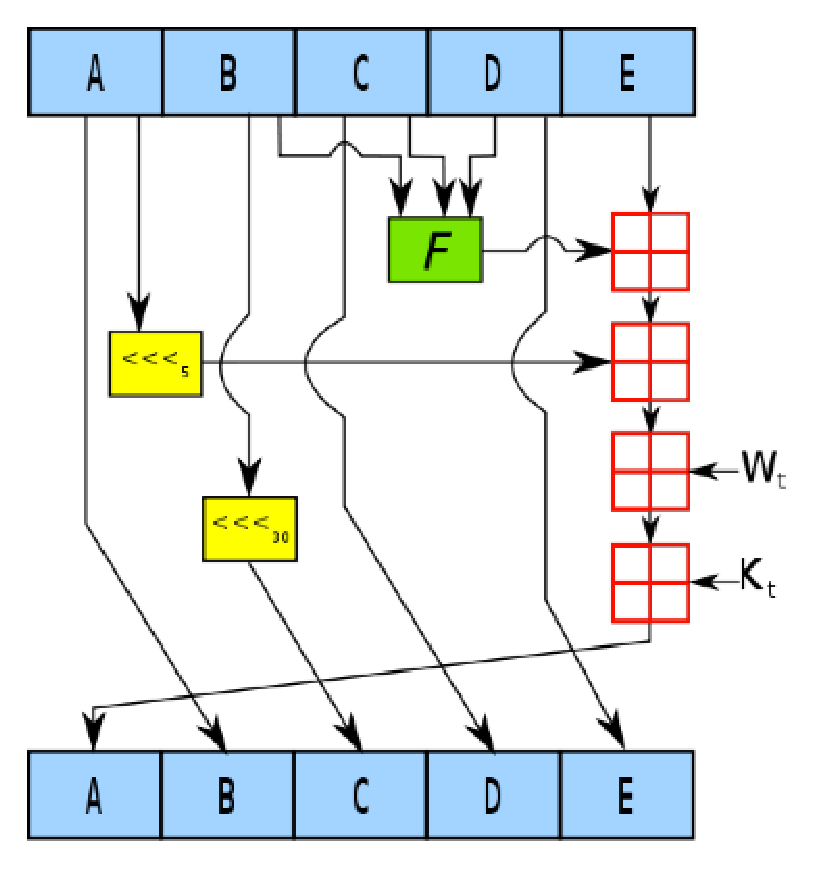
\includegraphics[scale=1.0]{eps/sha1pic.eps}
\caption{The SHA1 computation}
\label{sha1pic}
\end{figure}

\vspace{1mm}
\noindent
{\bf Portability Issues:}
SHA-1 is defined in terms of 32-bit ``words''.  This code
uses \verb|<stdint.h>| (included via ``sha1.h'' to define 32 and 8
bit unsigned integer types.  If your C compiler does not
support 32 bit unsigned integers, this code is not
appropriate.

\vspace{1mm}
\noindent
{\bf Caveats:}
SHA-1 is designed to work with messages less than $2^{64}$ bits
long.  Although SHA-1 allows a message digest to be generated
for messages of any number of bits less than $2^{64}$, this
implementation only works with messages with a length that is
a multiple of the size of an 8-bit character.

\vspace{1mm}
\noindent
See the RFC for SHA1\cite{30} and a video\cite{29} for details.
We use the C code specified in the RFC.

\begin{chunk}{includes}
#include <stdio.h>
#include <fcntl.h>
#include <stdint.h>

\end{chunk}

\begin{chunk}{enums}
enum
{
    shaSuccess = 0,
    shaNull,            /* Null pointer parameter */
    shaInputTooLong,    /* input data too long */
    shaStateError       /* called Input after Result */
};

\end{chunk}

\vspace{1mm}
\noindent
C \#defines
\begin{chunk}{defines}
#define SHA1HashSize 20
#define SHA1CircularShift(bits,word) \
                (((word) << (bits)) | ((word) >> (32-(bits))))


\end{chunk}

\subsection{The SHA1Context struct}
\index{SHA1Context}
\index{struct!SHA1Context}
\noindent
This structure will hold context information for the SHA-1 hashing operation
\begin{chunk}{SHA1Context}
typedef struct SHA1Context
{
 uint32_t Intermediate_Hash[SHA1HashSize/4]; /* Message Digest          */
 uint32_t Length_Low;               /* Message length in bits           */
 uint32_t Length_High;              /* Message length in bits           */
 int_least16_t Message_Block_Index; /* Index into message block array   */
 uint8_t Message_Block[64];         /* 512-bit message blocks           */
 int Computed;                      /* Is the digest computed?          */
 int Corrupted;                     /* Is the message digest corrupted? */
} SHA1Context;

\end{chunk}

\noindent
Function prototypes
\begin{chunk}{prototypes}
int SHA1Reset(  SHA1Context *);
int SHA1Input(  SHA1Context *, const uint8_t *, unsigned int);
int SHA1Result( SHA1Context *, uint8_t Message_Digest[SHA1HashSize]);
void SHA1PadMessage(SHA1Context *);
void SHA1ProcessMessageBlock(SHA1Context *);

\end{chunk}

\subsection{The SHA1Reset function}
\index{SHA1Reset}
\index{function!SHA1Reset}
\noindent
The {\bf SHA1Reset} function will initialize the SHA1Context in preparation
for computing a new SHA1 message digest. It modifies the {\bf context}
structure to contain the initial values.
\begin{chunk}{SHA1Reset}
int SHA1Reset(SHA1Context *context) {
  if (!context) {
    return shaNull;
  }
  context->Length_Low             = 0;
  context->Length_High            = 0;
  context->Message_Block_Index    = 0;
  context->Intermediate_Hash[0]   = 0x67452301;  /* H0 */
  context->Intermediate_Hash[1]   = 0xEFCDAB89;  /* H1 */
  context->Intermediate_Hash[2]   = 0x98BADCFE;  /* H2 */
  context->Intermediate_Hash[3]   = 0x10325476;  /* H3 */
  context->Intermediate_Hash[4]   = 0xC3D2E1F0;  /* H4 */
  context->Computed   = 0;
  context->Corrupted  = 0;
  return shaSuccess;
}

\end{chunk}

\subsection{The SHA1PadMessage function}
\index{SHA1PadMessage}
\index{function!SHA1PadMessage}
For {\bf SHA1PadMessage},the message must be padded to an even
512 bits. The first padding bit must be a '1'.  The last 64
bits represent the length of the original message.  All bits in
between should be 0.  This function will pad the message
according to those rules by filling the Message\_Block array
accordingly.  It will also call the 
{\bf ProcessMessageBlock} [\ref{ProcessMessageBlock}] function
provided appropriately.  When it returns, it can be assumed that
the message digest has been computed.

If the current message block is too small to hold the initial padding
bits and length then we will pad the block, process it, and then
continue padding into a second block.

\begin{chunk}{SHA1PadMessage}
void SHA1PadMessage(SHA1Context *context) {
  if (context->Message_Block_Index > 55) {
    context->Message_Block[context->Message_Block_Index++] = 0x80;
    while(context->Message_Block_Index < 64) {
      context->Message_Block[context->Message_Block_Index++] = 0;
    }
    SHA1ProcessMessageBlock(context);
    while(context->Message_Block_Index < 56) {
      context->Message_Block[context->Message_Block_Index++] = 0;
    }
  } else {
    context->Message_Block[context->Message_Block_Index++] = 0x80;
    while(context->Message_Block_Index < 56) {
     context->Message_Block[context->Message_Block_Index++] = 0;
    }
  }
  /* Store the message length as the last 8 octets */
  context->Message_Block[56] = context->Length_High >> 24;
  context->Message_Block[57] = context->Length_High >> 16;
  context->Message_Block[58] = context->Length_High >> 8;
  context->Message_Block[59] = context->Length_High;
  context->Message_Block[60] = context->Length_Low >> 24;
  context->Message_Block[61] = context->Length_Low >> 16;
  context->Message_Block[62] = context->Length_Low >> 8;
  context->Message_Block[63] = context->Length_Low;
  SHA1ProcessMessageBlock(context);
}

\end{chunk}

\subsection{The SHA1Result function}
\index{SHA1Result}
\index{function!SHA1Result}
The {\bf SHA1Result} will return the 160-bit message digest into the
Message\_Digest array  provided by the caller. 
NOTE: The first octet of hash is stored in the 0th element,
the last octet of hash in the 19th element.
\begin{chunk}{SHA1Result}
int SHA1Result( SHA1Context *context, uint8_t Message_Digest[SHA1HashSize]) {
  int i;
  if (!context || !Message_Digest) {
    return shaNull;
  }
  if (context->Corrupted) {
    return context->Corrupted;
  }
  if (!context->Computed) {
    SHA1PadMessage(context);
    for(i=0; i<64; ++i) {
      context->Message_Block[i] = 0; /* message may be sensitive, clear it */
    }
    context->Length_Low = 0;         /* and clear length */
    context->Length_High = 0;
    context->Computed = 1;
  }
  for(i = 0; i < SHA1HashSize; ++i) {
    Message_Digest[i] = 
      context->Intermediate_Hash[i>>2] >> 8 * ( 3 - ( i & 0x03 ) );
  }
  return shaSuccess;
}

\end{chunk}

\subsection{The SHA1ProcessMessageBlock function}
\label{ProcessMessageBlock}
\index{SHA1ProcessMessageBlock}
\index{function!SHA1ProcessMessageBlock}
The {\bf SHA1ProcessMessageBlock} will process the next 512 bits 
of the message stored in the Message\_Block array.
Note that single character names were used because those were the
names used in the publication.
\begin{chunk}{SHA1ProcessMessageBlock}
void SHA1ProcessMessageBlock(SHA1Context *context) {
  const uint32_t K[] = { 0x5A827999, 0x6ED9EBA1, 0x8F1BBCDC, 0xCA62C1D6 };
                              /* Constants defined in SHA-1  */
  int t;                      /* Loop counter                */
  uint32_t temp;              /* Temporary word value        */
  uint32_t W[80];             /* Word sequence               */
  uint32_t A, B, C, D, E;     /* Word buffers                */
  for(t = 0; t < 16; t++) {
    W[t] = context->Message_Block[t * 4] << 24;
    W[t] |= context->Message_Block[t * 4 + 1] << 16;
    W[t] |= context->Message_Block[t * 4 + 2] << 8;
    W[t] |= context->Message_Block[t * 4 + 3];
  }
  for(t = 16; t < 80; t++) {
    W[t] = SHA1CircularShift(1,W[t-3] ^ W[t-8] ^ W[t-14] ^ W[t-16]);
  }
  A = context->Intermediate_Hash[0];
  B = context->Intermediate_Hash[1];
  C = context->Intermediate_Hash[2];
  D = context->Intermediate_Hash[3];
  E = context->Intermediate_Hash[4];
  for(t = 0; t < 20; t++) {
    temp =  SHA1CircularShift(5,A) + ((B & C) | ((~B) & D)) + E + W[t] + K[0];
    E = D;
    D = C;
    C = SHA1CircularShift(30,B);
    B = A;
    A = temp;
  }
  for(t = 20; t < 40; t++) {
    temp = SHA1CircularShift(5,A) + (B ^ C ^ D) + E + W[t] + K[1];
    E = D;
    D = C;
    C = SHA1CircularShift(30,B);
    B = A;
    A = temp;
  }
  for(t = 40; t < 60; t++) {
    temp = SHA1CircularShift(5,A)+((B & C) | (B & D) | (C & D))+E+W[t]+K[2];
    E = D;
    D = C;
    C = SHA1CircularShift(30,B);
    B = A;
    A = temp;
  }
  for(t = 60; t < 80; t++) {
    temp = SHA1CircularShift(5,A) + (B ^ C ^ D) + E + W[t] + K[3];
    E = D;
    D = C;
    C = SHA1CircularShift(30,B);
    B = A;
    A = temp;
  }
  context->Intermediate_Hash[0] += A;
  context->Intermediate_Hash[1] += B;
  context->Intermediate_Hash[2] += C;
  context->Intermediate_Hash[3] += D;
  context->Intermediate_Hash[4] += E;
  context->Message_Block_Index = 0;
}

\end{chunk}

\subsection{The SHA1Input function}
\index{SHA1Input}
\index{function!SHA1Input}
The {\bf SHA1Input} accepts an array of octets as the next portion
of the message. The {\bf context} contains the SHA context to update.
The {\bf message\_array} contains the array of characters representing 
the next portion of the message. The {\bf length} is the length of
the message\_array.
\begin{chunk}{SHA1Input}
int SHA1Input(SHA1Context    *context,
              const uint8_t  *message_array,
              unsigned       length) {
  if (!length) {
    return shaSuccess;
  }
  if (!context || !message_array) {
    return shaNull;
  }
  if (context->Computed) {
    context->Corrupted = shaStateError;
    return shaStateError;
  }
  if (context->Corrupted) {
     return context->Corrupted;
  }
  while(length-- && !context->Corrupted) {
    context->Message_Block[context->Message_Block_Index++] =
                  (*message_array & 0xFF);
    context->Length_Low += 8;
    if (context->Length_Low == 0) {
      context->Length_High++;
      if (context->Length_High == 0) {
        context->Corrupted = 1;   /* Message is too long */
      }
    }
    if (context->Message_Block_Index == 64) {
      SHA1ProcessMessageBlock(context);
    }
    message_array++;
  }
  return shaSuccess;
}

\end{chunk}

\subsection{The processFile function}
\index{processFile}
\index{function!processFile}
\noindent
The {\bf processFile} function assumes that the files are {\bf open}
for {\bf binary} reading and writing. It copies the bytes. In a
successful copy, {\bf outcount} will end up 0. 
\begin{chunk}{processfile}
int processfile(FILE* input, FILE* output) {
  unsigned char buffer[1024];
  size_t incount;
  size_t outcount;
  do {
    incount = fread(buffer,sizeof(unsigned char),sizeof(buffer),input);
    if (incount) {
      outcount = fwrite(buffer,1,incount,output); 
    } else {
      outcount = 0;
    }
  } while ((incount > 0) && (incount == outcount));
  return outcount;
}

\end{chunk} 

\subsection{The RFC test set}
\index{RFCtest}
\index{function!RFCtest}
\noindent
The {\bf RFCtest} function runs the test code specified in RFC 3174\cite{30}.
This will exercise the SHA-1 code performing the three
tests documented in FIPS PUB 180-1 plus one which calls
SHA1Input with an exact multiple of 512 bits, plus a few
error test checks.
\begin{chunk}{rfctest.c}
#include <string.h>
\getchunk{includes}
\getchunk{enums}
\getchunk{defines}
\getchunk{SHA1Context}
\getchunk{prototypes}
\getchunk{SHA1Reset}
\getchunk{SHA1PadMessage}
\getchunk{SHA1Result}
\getchunk{SHA1ProcessMessageBlock}
\getchunk{SHA1Input}

/* Define patterns for testing */
#define TEST1   "abc"
#define TEST2a  "abcdbcdecdefdefgefghfghighijhi"
#define TEST2b  "jkijkljklmklmnlmnomnopnopq"
#define TEST2   TEST2a TEST2b
#define TEST3   "a"
#define TEST4a  "01234567012345670123456701234567"
#define TEST4b  "01234567012345670123456701234567"
/* an exact multiple of 512 bits */
#define TEST4   TEST4a TEST4b
char *testarray[4] = { TEST1, TEST2, TEST3, TEST4 };
long int repeatcount[4] = { 1, 1, 1000000, 10 };
char *resultarray[4] = {
    "A9 99 3E 36 47 06 81 6A BA 3E 25 71 78 50 C2 6C 9C D0 D8 9D",
    "84 98 3E 44 1C 3B D2 6E BA AE 4A A1 F9 51 29 E5 E5 46 70 F1",
    "34 AA 97 3C D4 C4 DA A4 F6 1E EB 2B DB AD 27 31 65 34 01 6F",
    "DE A3 56 A2 CD DD 90 C7 A7 EC ED C5 EB B5 63 93 4F 46 04 52"
};

int main() {
  SHA1Context sha;
  int i, j, err;
  uint8_t Message_Digest[20];
  for(j = 0; j < 4; ++j) {
    printf( "\nTest %d: %ld, '%s'\n", j+1, repeatcount[j], testarray[j]);
    err = SHA1Reset(&sha);
    if (err) {
      fprintf(stderr, "SHA1Reset Error %d.\n", err );
      break; /* out of for j loop */
    }
    for(i = 0; i < repeatcount[j]; ++i) {
      err = SHA1Input(&sha,
                      (const unsigned char *) testarray[j],
                      strlen(testarray[j]));
      if (err) {
        fprintf(stderr, "SHA1Input Error %d.\n", err );
        break;    /* out of for i loop */
      }
    }
    err = SHA1Result(&sha, Message_Digest);
    if (err) {
      fprintf(stderr,
             "SHA1Result Error %d, could not compute message digest.\n",
             err );
    } else {
      printf("\t");
      for(i = 0; i < 20 ; ++i) {
        printf("%02X ", Message_Digest[i]);
      }
      printf("\n");
    }
    printf("Should match:\n");
    printf("\t%s\n", resultarray[j]);
  }
  /* Test some error returns */
  err = SHA1Input(&sha,(const unsigned char *) testarray[1], 1);
  printf ("\nError %d. Should be %d.\n", err, shaStateError );
  err = SHA1Reset(0);
  printf ("\nError %d. Should be %d.\n", err, shaNull );
  return 0;
}

\end{chunk}

\subsection{The main function}
\index{main}
\index{function!main}
\noindent
The {\bf main} function opens the file, processes it, and exits.
This is the command line entry purely for testing. The full program
will use functions from the API.
\begin{chunk}{sha1.c}

\getchunk{includes}
\getchunk{enums}
\getchunk{defines}
\getchunk{SHA1Context}
\getchunk{prototypes}
\getchunk{SHA1Reset}
\getchunk{SHA1PadMessage}
\getchunk{SHA1Result}
\getchunk{SHA1ProcessMessageBlock}
\getchunk{SHA1Input}
\getchunk{processfile}

int main(int argc, char *argv[]) {
  FILE *input;
  FILE *output;
  int outcount = 0;
  if (argc != 3 || strcmp(argv[1],"--help") == 0) {
    printf("sha1 inputFilename outputFilename");
  }
  if ( (input = fopen(argv[1],"rb")) == NULL) {
    printf("sha1: %s file not found\n",argv[1]);
    return -1;
  }
  if ( (output = fopen(argv[2],"wb")) == NULL) {
    printf("sha1: could not open output file %s\n",argv[2]);
    return -2;
  }
  if ( (outcount = processfile(input,output)) != 0) {
    printf("sha1: binary copy from %s to %s failed\n",argv[1],argv[2]);
    return outcount;
  }
  if (fclose(output)) {
    printf("sha1: could not close %s\n",argv[2]);
    return -3;
  }
  if (fclose(input)) {
    printf("sha1: could not close %s\n",argv[1]);
    return -4;
  }
  return 0;
}

\end{chunk}



\chapter{FTP Details}

In this part, upon the two-ubuntu LAN that we built previously, we use
FTP (File transfer protocol) to transfer a 7353 bytes file from host
to server. And using Wireshark, I will give a detailed analysis on how
the ftp files break into packets and into bits.

\begin{figure}[ht!]
\centering
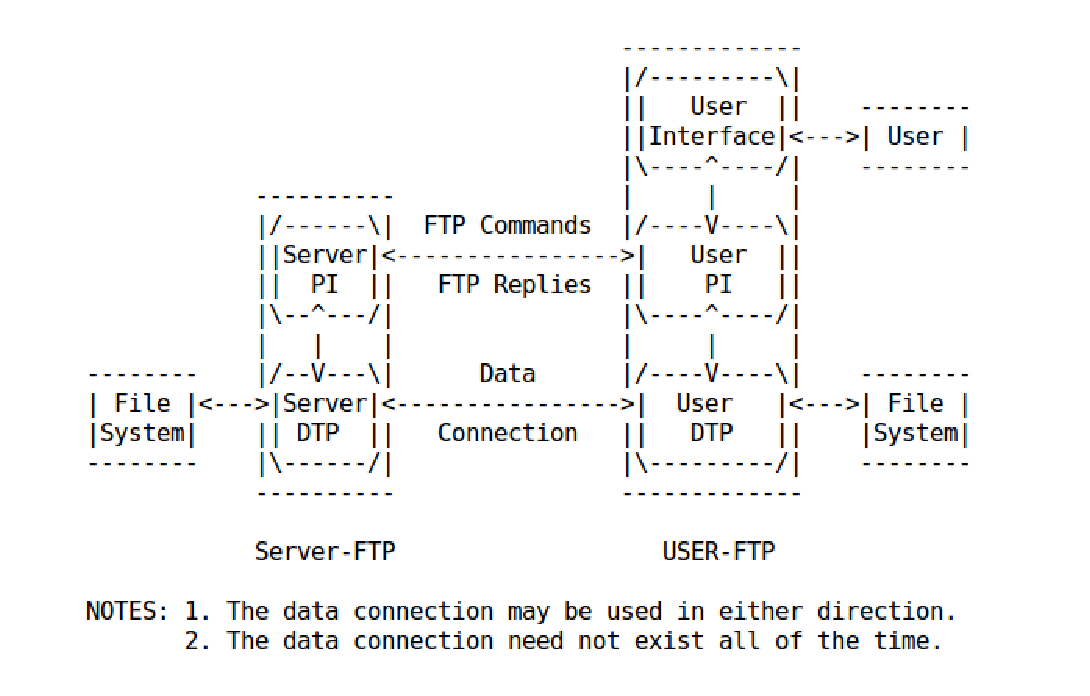
\includegraphics[scale=0.75]{eps/ftp-model.eps}
\caption{The FTP model}
\label{ftp-model}
\end{figure}

As can be seen in Figure~\ref{ftp-model}, the data connection is established
between the server DTP (data transfer process) and the user DTP, as
for ftp commands and replies, they are transfered between server PI
(protocol interpreter) and user PI.

\begin{figure}[ht!]
\centering
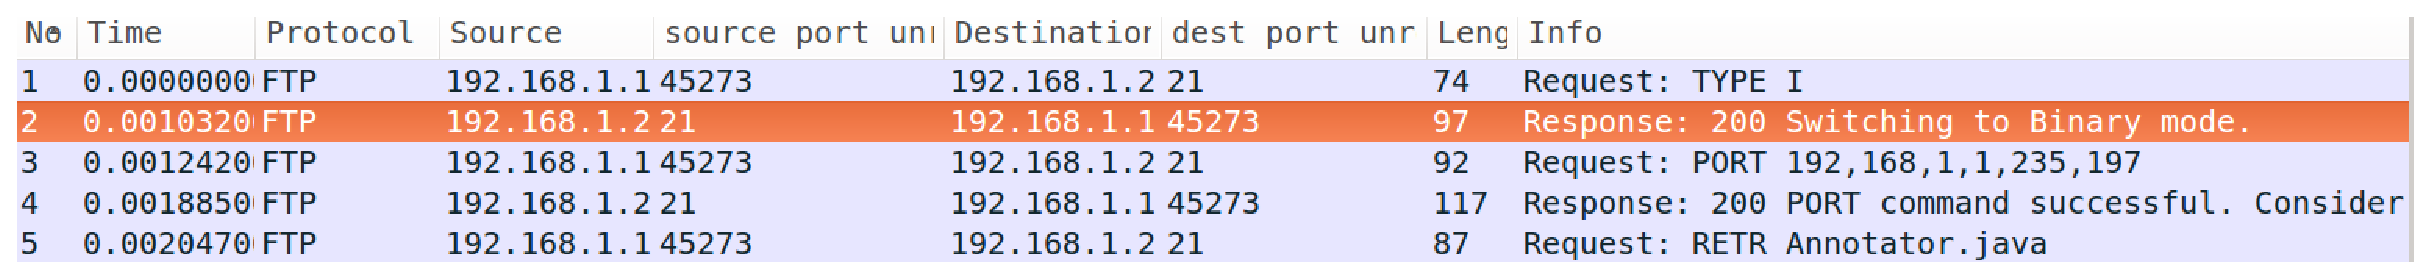
\includegraphics[scale=0.35]{eps/ftp1.eps}
\caption{FTP data connection establishment}
\label{ftp1}
\end{figure}

Figure~\ref{ftp1} shows a typical ftp data connection establishment. 
\begin{enumerate}
\item host request server for connection.
\item server responses code 200, meaning that connection permmitted.
\item and port 179,6 (45830) is to be used
\item use PASV, a mode where the client initiates the data connection.
\item ready to return the aimed file Annotator.java.
\end{enumerate}

\begin{figure}[ht!]
\centering
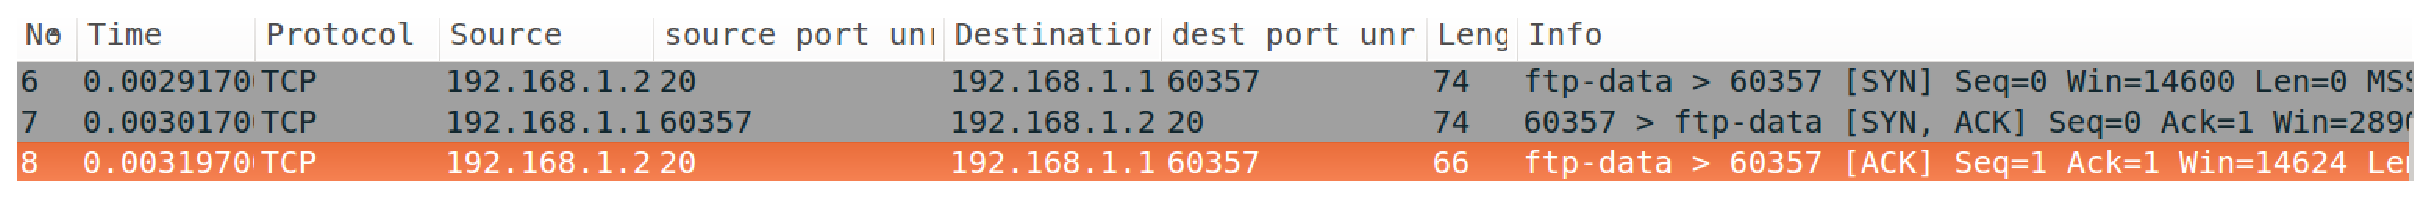
\includegraphics[scale=0.35]{eps/ftp2.eps}
\caption{A 3-way TCP handshake}
\label{ftp2}
\end{figure}

Figure~\ref{ftp2} is a typical 3-way-hand-shaking TCP, to synthesize and
establish a reliable connection.

\begin{figure}[ht!]
\centering
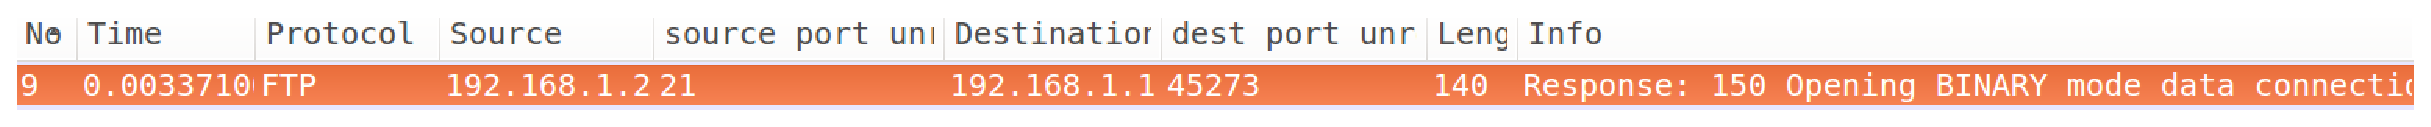
\includegraphics[scale=0.35]{eps/ftp3.eps}
\caption{File status okay, open data connection}
\label{ftp3}
\end{figure}

Figure~\ref{ftp3} shows that, code 150 means "File status okay; about to open
data connection."

\begin{figure}[ht!]
\centering
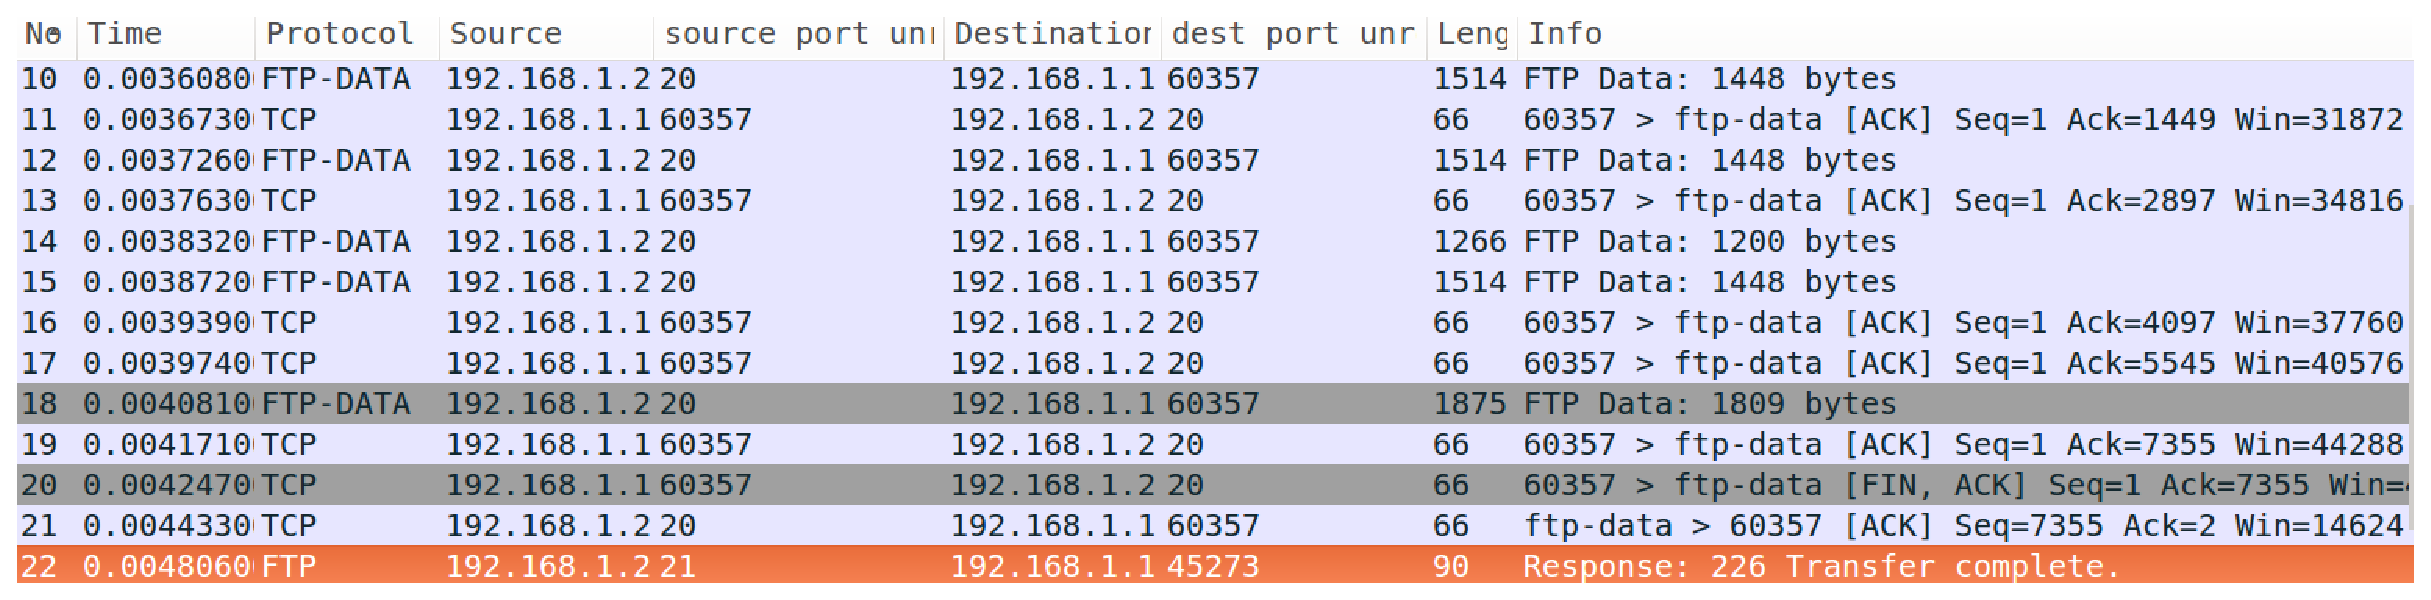
\includegraphics[scale=0.35]{eps/ftp4.eps}
\caption{File transfer}
\label{ftp4}
\end{figure}

In Figure~\ref{ftp4} 
we come to the file transfers, we can see that the files are
transferred in several parts, and after each part of data transferred
into user, user would send an ACK (acknowledgement) back to server,
meaning that the user received the data successfully. At the end, code
226 means "Closing data connection. Requested file action successful
(for example, file transfer or file abort)."

\begin{figure}[ht!]
\centering
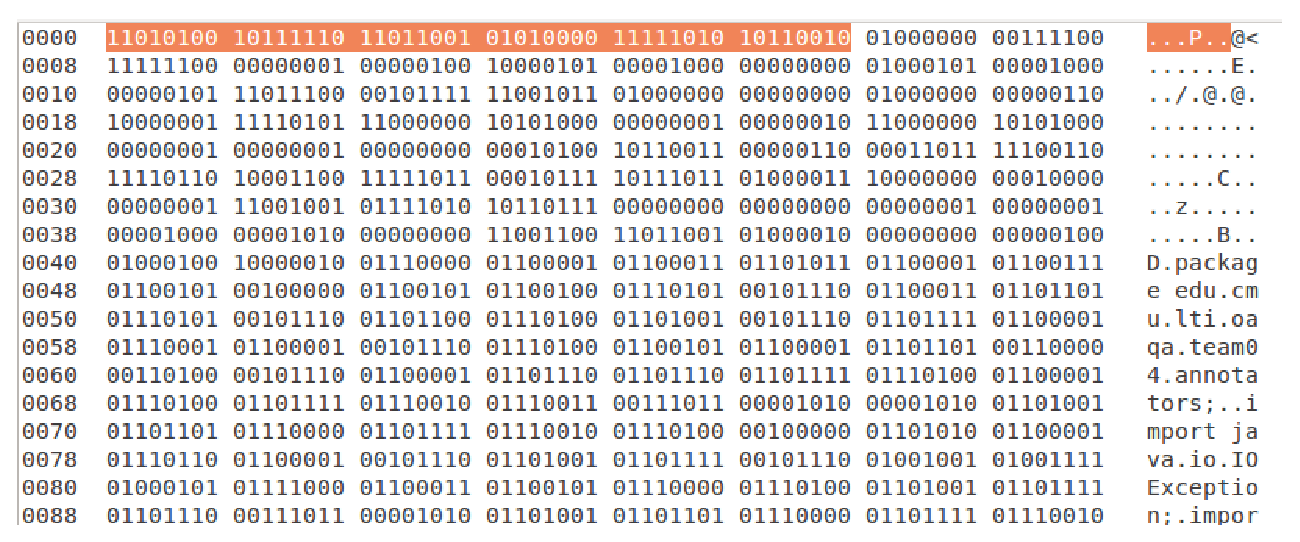
\includegraphics[scale=0.65]{eps/ftp5.eps}
\caption{An FTP data packet}
\label{ftp5}
\end{figure}

Figure~\ref{ftp5} shows one of the ftp-data packet, where bits of the packet
can be seen.

First, how can we know if the packet is the ftp-data packet? We can
check the source port (20 as ftp data) and destination port, and in
the meantime check if there are bits after 66 bytes. (We will see the
code inplementation of this soon)

Thus, similarly, for every ftp-data packet, we can grab those bits of
data from the 66 bytes of the packet to the end.

Now let's look into the bits of one of the ftp-data packet of the file
(Annotator.java).

\begin{figure}[ht!]
\centering
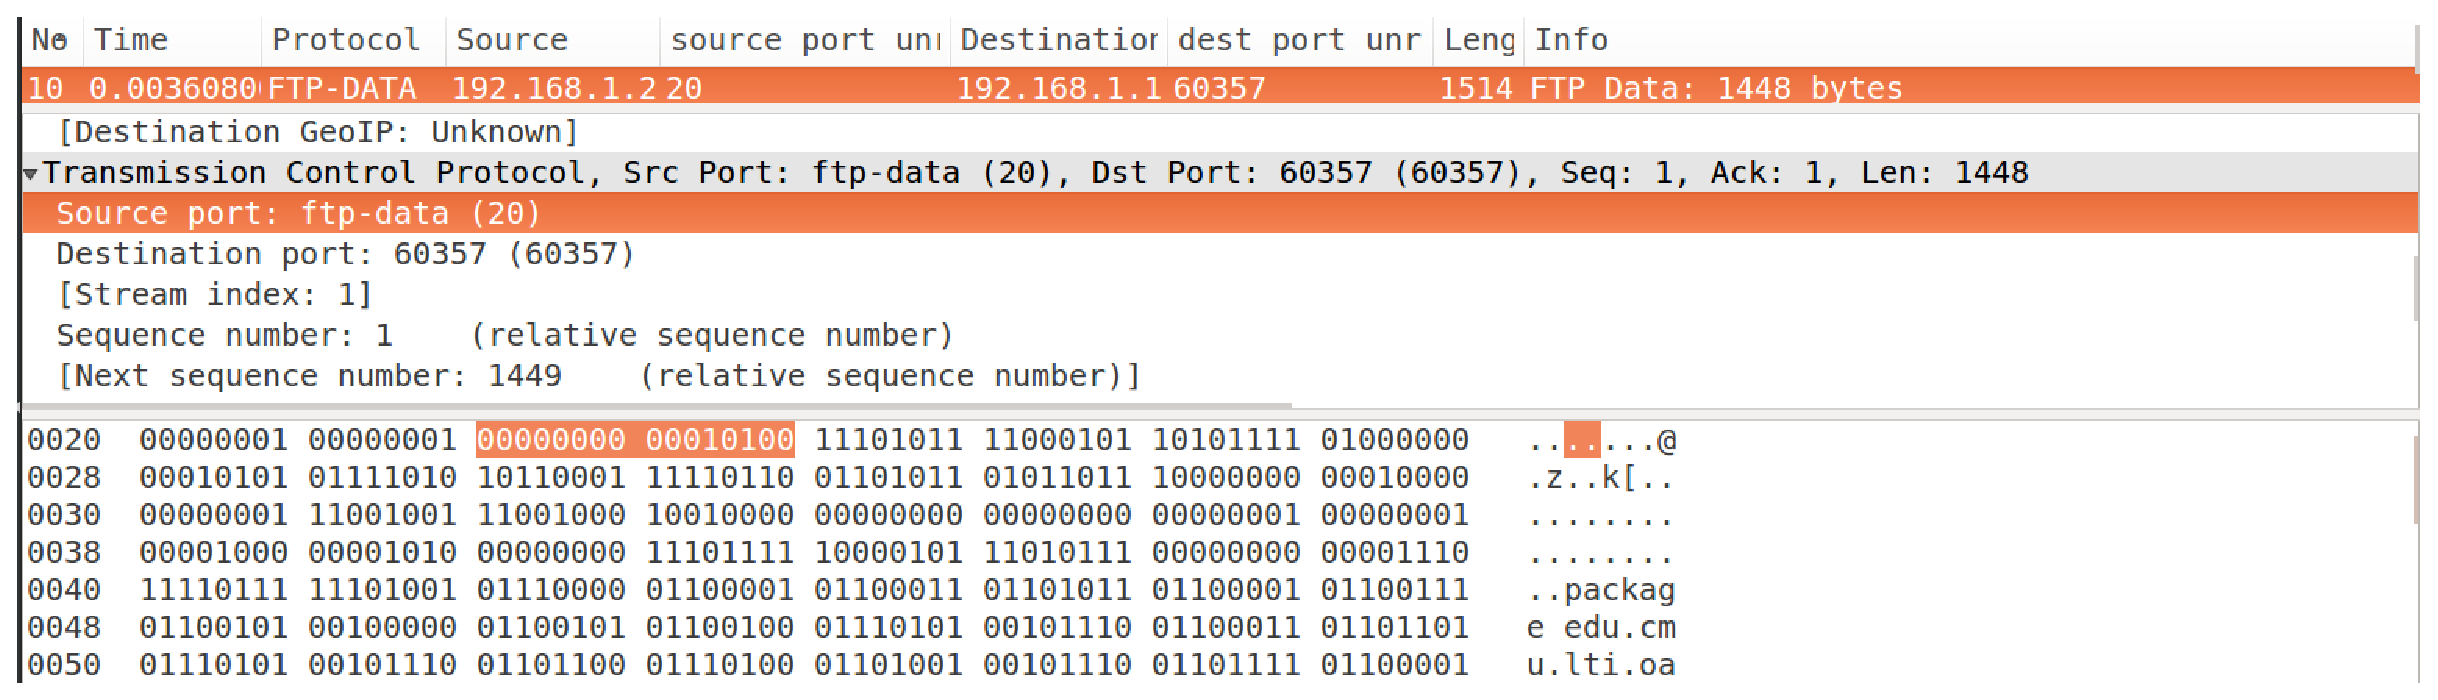
\includegraphics[scale=0.35]{eps/ftp6.eps}
\caption{Details}
\label{ftp6}
\end{figure}

Figure~\ref{ftp6}, figure~\ref{ftp7}, figure~\ref{ftp8}, and 
figure~\ref{ftp9} 
show the details for a packet. 

\newpage
For each packet:

\begin{figure}[ht!]
\centering
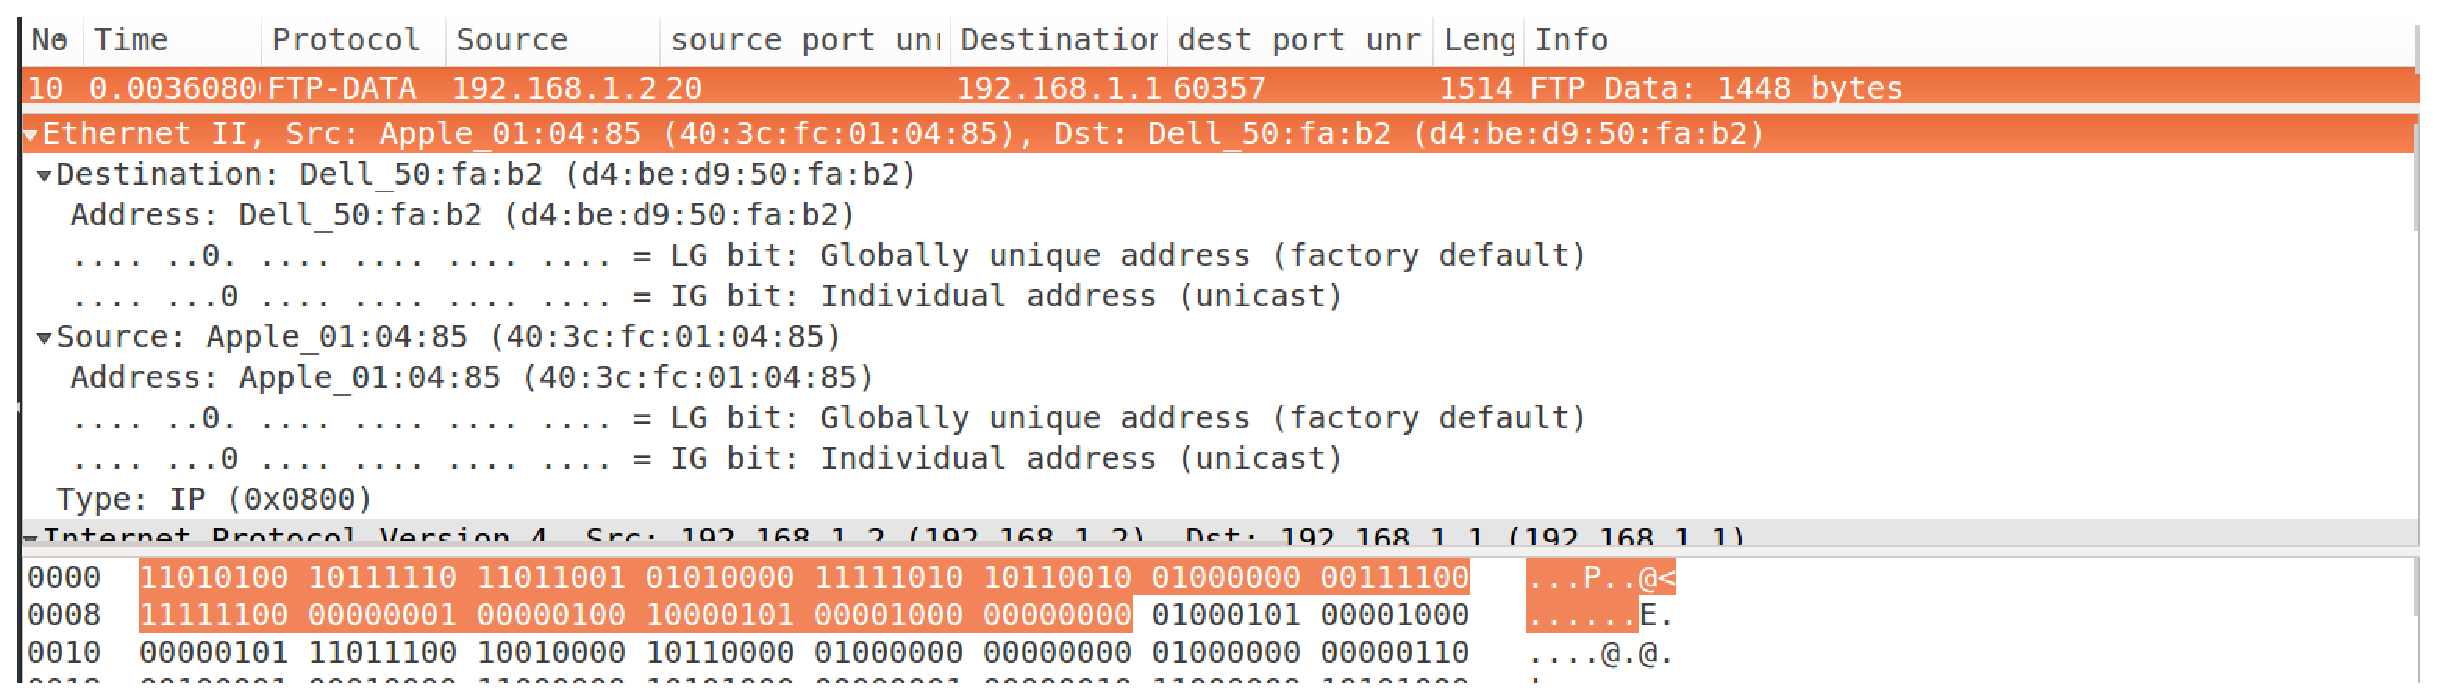
\includegraphics[scale=0.35]{eps/ftp7.eps}
\caption{Bit level details}
\label{ftp7}
\end{figure}

\begin{enumerate}
\item {\bf bytes 0-5} first 6 bytes are user mac 
address (d4:be:d9:50:fa:b2 here)

\begin{chunk}{get dest mac addr}
/*got to write this*/
\end{chunk}

{\bf bytes 6-11} (6) bytes are server mac 
address (40:3c:fc:01:04:85), 

{\bf bytes 12-13} (2) bytes are IP (0X0800).

\newpage
\begin{figure}[ht!]
\centering
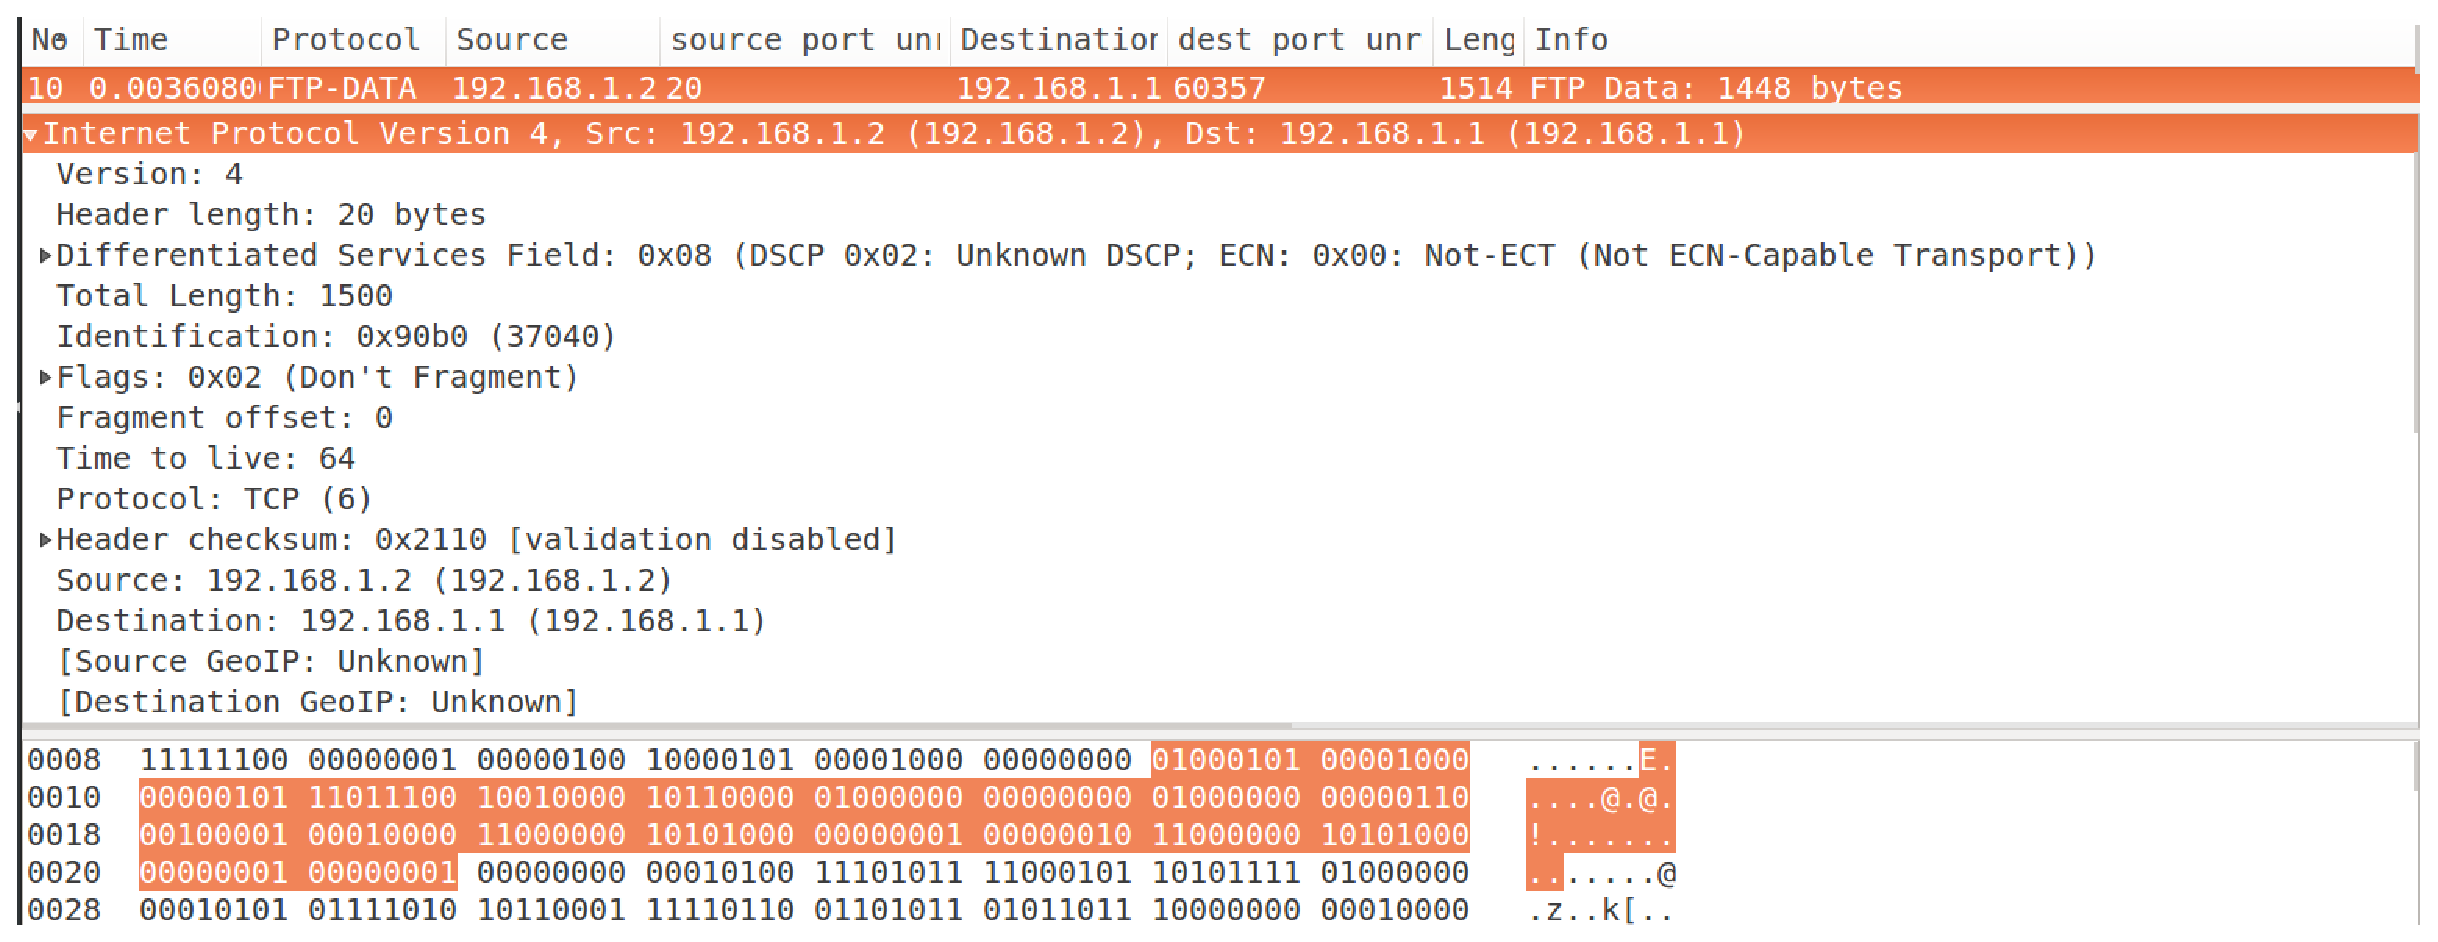
\includegraphics[scale=0.35]{eps/ftp8.eps}
\caption{More bit level details}
\label{ftp8}
\end{figure}

\item {\bf byte 14} is header length (20), 

{\bf byte 15} is the tag byte, 

{\bf bytes 16-17} (2) bytes are total length of data transferred (1500), 

{\bf bytes 18-19} (2) bytes are identification (0x2fcb $->$ 12235), 

{\bf bytes 20-21} (2) bytes are fragment offset (0), 

{\bf byte 22} is time to live (64), 

{\bf byte 23} is protocol used (6 $->$ TCP),

{\bf bytes 24-25} (2) bytes are header checksum 
(0x81f5 $->$ validation disabled),

{\bf bytes 26-29} (4) bytes are source GeoIP (unknown), 

{\bf bytes 30-33} (4) bytes are destination GeoIP (unknown).

\newpage
\begin{figure}[ht!]
\centering
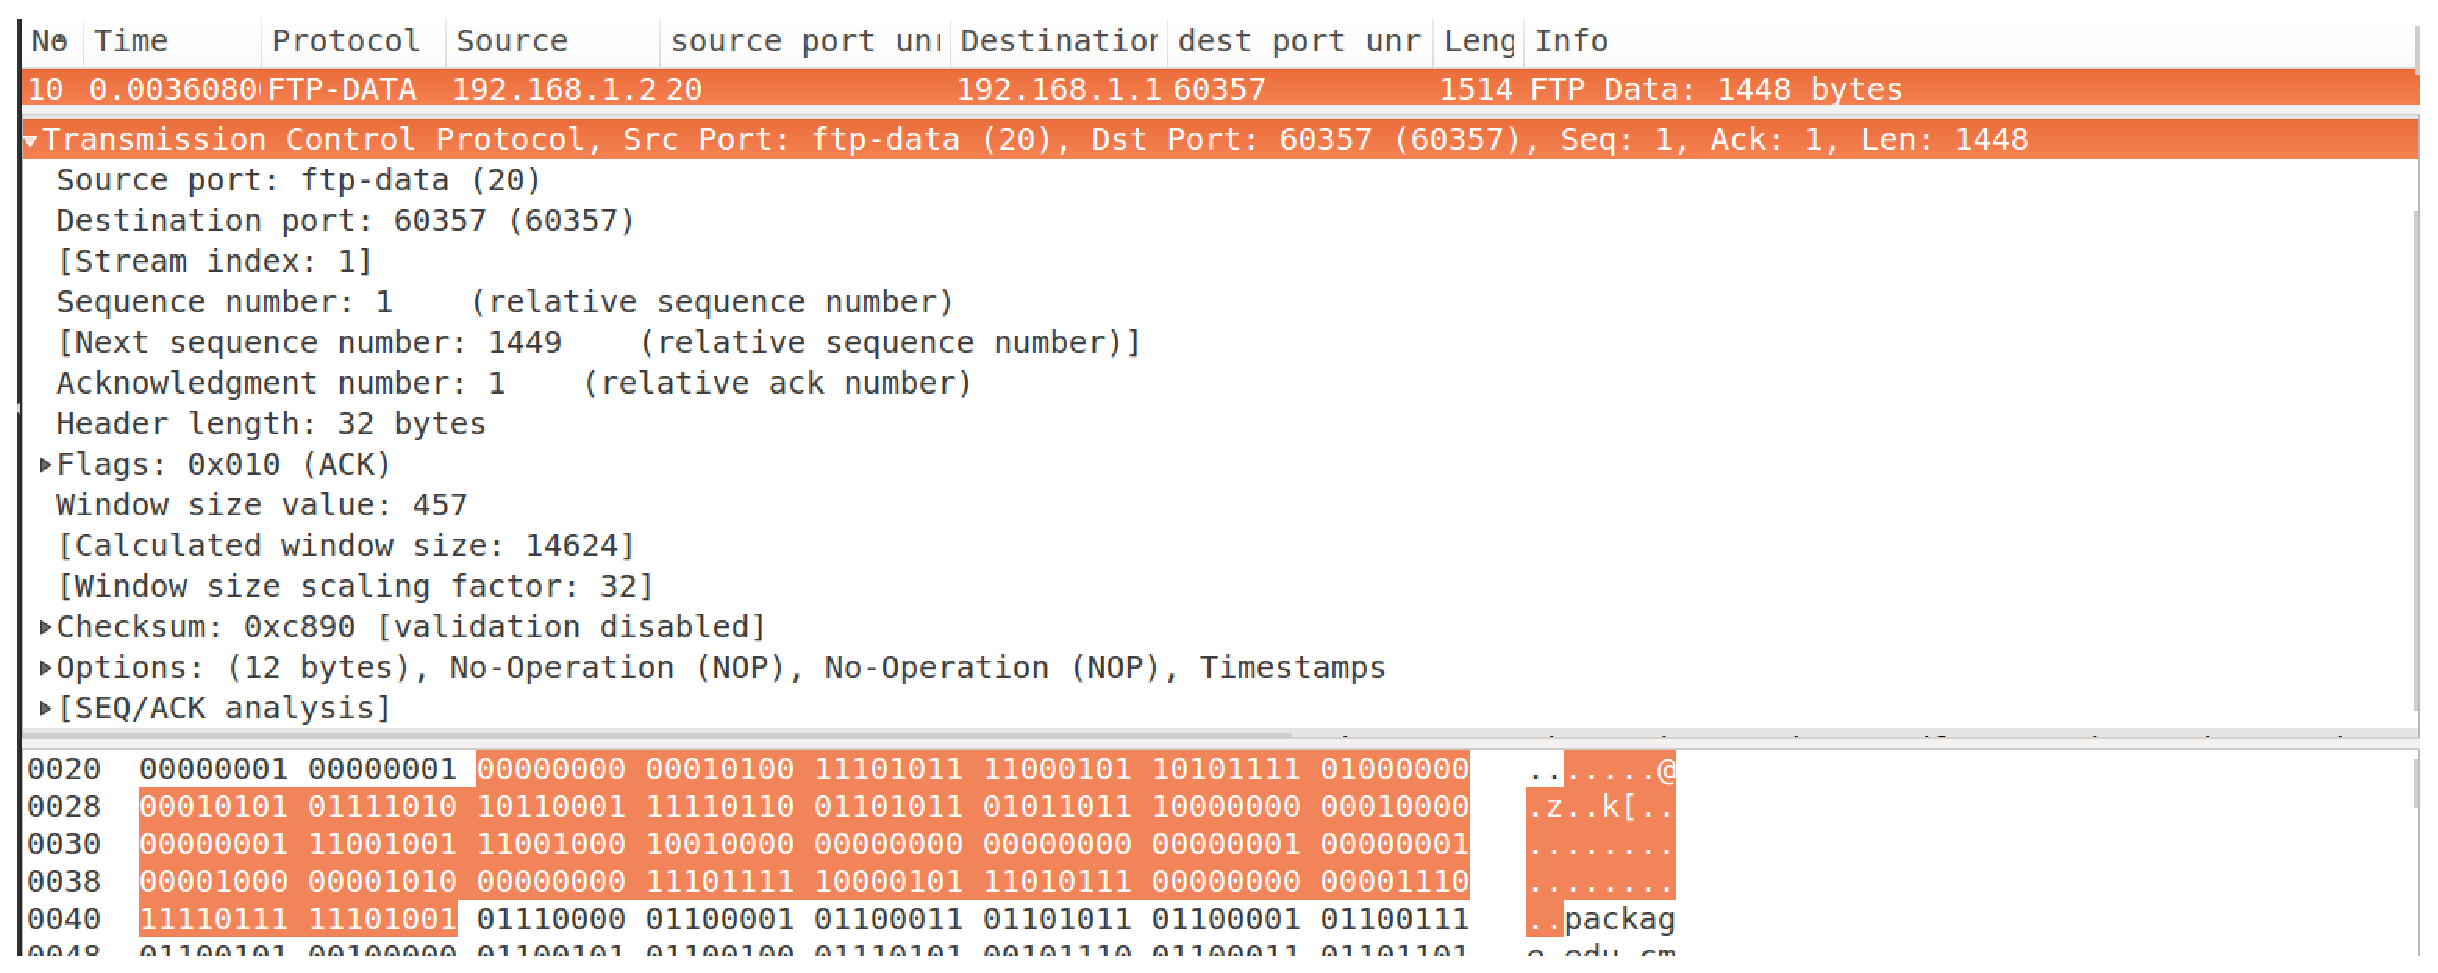
\includegraphics[scale=0.35]{eps/ftp9.eps}
\caption{More bit level details}
\label{ftp9}
\end{figure}

\item {\bf bytes 34-35} (2) bytes are source port (20 $->$ ftp-data port), 

{\bf bytes 36-37} (2) bytes are destination port (45830), 

{\bf bytes 38-41} (4) bytes are sequence number (1), 

{\bf bytes 42-45} (4) bytes are acknowledgment number (1), 

{\bf bytes 46-47} (2) bytes are flags (0x010), 

{\bf bytes 48-49} (2) bytes are window size value and scaling factor, 

{\bf bytes 50-51} (2) bytes are checksum (0x7ab7 $->$ validation
disabled), 

{\bf bytes 52-61} all belong to TCP, 

{\bf bytes 62-65} (4) bytes are timestamp echo reply (279682).

\item then we see our data (1448 bytes), 
which takes a large part of the packet.
\end{enumerate}

Thus, this analysis gives us the hint of how to abstract the bits of
the file out of the packets flow.

A packet analyzer (also known as a network analyzer, protocol analyzer
or packet sniffer—or, for particular types of networks, an Ethernet
sniffer or wireless sniffer) is a computer program or piece of
computer hardware that can intercept and log traffic that passes over
a digital network or part of a network. As data streams flow across
the network, the sniffer captures each packet and, if needed, decodes
the packet's raw data, showing the values of various fields in the
packet, and analyzes its content according to the appropriate RFC or
other specifications. \cite{39} Wireshark for example is the most
popular packet sniffer out there and is available for all
platforms. Its gui based and very easy to use.

In this chapter we are going to talk about how to code and make our own packet sniffer in C and on the linux platform. 

Note that it sniffs only incoming packets.

\begin{chunk}{includes}
#include<stdio.h> //For standard things
#include<stdlib.h>    //malloc
#include<string.h>    //memset
//can get
#include<netinet/tcp.h>   //Provides declarations for tcp header
//can get
#include<netinet/ip.h>    //Provides declarations for ip header
#include<sys/socket.h>
#include<arpa/inet.h>

\end{chunk}

\begin{chunk}{About the sockaddrin struct}
struct sockaddr_in{
  short sin_family;
  unsigned short sin_port;
  IN_ADDR sin_addr;
  char sin_zero[8];
};
members in struct:
sin_family
    Address family; must be AF_INET.
sin_port
    Internet Protocol (IP) port.
sin_addr
    IP address in network byte order.
sin_zero
    Padding to make structure the same size as SOCKADDR.
\end{chunk}

\begin{chunk}{globalVs}
int sock_raw;
FILE *logfile;
int tcp=0,others=0,total=0,i,j;
struct sockaddr_in source,dest;

\end{chunk}

\noindent
Function prototypes
\begin{chunk}{prototypes}
void ProcessPacket(unsigned char* , int);
void printipheader(unsigned char* , int);
void printtcppacket(unsigned char* , int);
void PrintData (unsigned char* , int);

\end{chunk}

\subsection{The ProcessPacket function}
\index{ProcessPacket}
\index{function!ProcessPacket}
\noindent
In this ProcessPacket function, we:

1. get the IP header part of the packet.
2. check the protocol and see if it's tcp in this case
3. if it's tcp, then print the packet in tcp format

\begin{chunk}{ProcessPacket}
void ProcessPacket(unsigned char* buffer, int size)
{
    //Get the IP Header part of this packet
    struct iphdr *iph = (struct iphdr*)buffer;
    ++total;
    switch (iph->protocol) //Check the Protocol and do accordingly...
    { 
        case 6:  //TCP Protocol
            ++tcp;
            printtcppacket(buffer , size);
            break;
         
        default: //Some Other Protocol like ARP etc.
            ++others;
            break;
    }
    printf("TCP : %d   Others : %d   Total : %d\r",tcp,others,total);
}

\end{chunk}

\subsection{The printipheader function}
\index{printipheader}
\index{function!printipheader}
For {\bf printipheader}, 

\begin{chunk}{printipheader}
void printipheader(unsigned char* Buffer, int Size)
{
    unsigned short iphdrlen;
         
    struct iphdr *iph = (struct iphdr *)Buffer;
    iphdrlen =iph->ihl*4;
     
    memset(&source, 0, sizeof(source));
    source.sin_addr.s_addr = iph->saddr;
     
    memset(&dest, 0, sizeof(dest));
    dest.sin_addr.s_addr = iph->daddr;
     
    fprintf(logfile,"\n");
    fprintf(logfile,"IP Header\n");
    fprintf(logfile,"   |-IP Version        : %d\n",(unsigned int)iph->version);
    fprintf(logfile,"   |-IP Header Length  : %d DWORDS or %d Bytes\n",(unsigned int)iph->ihl,((unsigned int)(iph->ihl))*4);
    fprintf(logfile,"   |-Type Of Service   : %d\n",(unsigned int)iph->tos);
    fprintf(logfile,"   |-IP Total Length   : %d  Bytes(Size of Packet)\n",ntohs(iph->tot_len));
    fprintf(logfile,"   |-Identification    : %d\n",ntohs(iph->id));
    //fprintf(logfile,"   |-Reserved ZERO Field   : %d\n",(unsigned int)iphdr->ip_reserved_zero);
    //fprintf(logfile,"   |-Dont Fragment Field   : %d\n",(unsigned int)iphdr->ip_dont_fragment);
    //fprintf(logfile,"   |-More Fragment Field   : %d\n",(unsigned int)iphdr->ip_more_fragment);
    fprintf(logfile,"   |-TTL      : %d\n",(unsigned int)iph->ttl);
    fprintf(logfile,"   |-Protocol : %d\n",(unsigned int)iph->protocol);
    fprintf(logfile,"   |-Checksum : %d\n",ntohs(iph->check));
    fprintf(logfile,"   |-Source IP        : %s\n",inet_ntoa(source.sin_addr));
    fprintf(logfile,"   |-Destination IP   : %s\n",inet_ntoa(dest.sin_addr));
}

\end{chunk}

\subsection{The printtcppacket function}
\index{printtcppacket}
\index{function!printtcppacket}
The {\bf printtcppacket} will 
\begin{chunk}{printtcppacket}
void printtcppacket(unsigned char* Buffer, int Size)
{
    unsigned short iphdrlen;
     
    struct iphdr *iph = (struct iphdr *)Buffer;
    iphdrlen = iph->ihl*4;
     
    struct tcphdr *tcph=(struct tcphdr*)(Buffer + iphdrlen);
             
    fprintf(logfile,"\n\n***********************TCP Packet*************************\n");   
         
    printipheader(Buffer,Size);
         
    fprintf(logfile,"\n");
    fprintf(logfile,"TCP Header\n");
    fprintf(logfile,"   |-Source Port      : %u\n",ntohs(tcph->source));
    fprintf(logfile,"   |-Destination Port : %u\n",ntohs(tcph->dest));
    fprintf(logfile,"   |-Sequence Number    : %u\n",ntohl(tcph->seq));
    fprintf(logfile,"   |-Acknowledge Number : %u\n",ntohl(tcph->ack_seq));
    fprintf(logfile,"   |-Header Length      : %d DWORDS or %d BYTES\n" ,(unsigned int)tcph->doff,(unsigned int)tcph->doff*4);
    //fprintf(logfile,"   |-CWR Flag : %d\n",(unsigned int)tcph->cwr);
    //fprintf(logfile,"   |-ECN Flag : %d\n",(unsigned int)tcph->ece);
    fprintf(logfile,"   |-Urgent Flag          : %d\n",(unsigned int)tcph->urg);
    fprintf(logfile,"   |-Acknowledgement Flag : %d\n",(unsigned int)tcph->ack);
    fprintf(logfile,"   |-Push Flag            : %d\n",(unsigned int)tcph->psh);
    fprintf(logfile,"   |-Reset Flag           : %d\n",(unsigned int)tcph->rst);
    fprintf(logfile,"   |-Synchronise Flag     : %d\n",(unsigned int)tcph->syn);
    fprintf(logfile,"   |-Finish Flag          : %d\n",(unsigned int)tcph->fin);
    fprintf(logfile,"   |-Window         : %d\n",ntohs(tcph->window));
    fprintf(logfile,"   |-Checksum       : %d\n",ntohs(tcph->check));
    fprintf(logfile,"   |-Urgent Pointer : %d\n",tcph->urg_ptr);
    fprintf(logfile,"\n");
    fprintf(logfile,"                        DATA Dump                         ");
    fprintf(logfile,"\n");
         
    fprintf(logfile,"IP Header\n");
    PrintData(Buffer,iphdrlen);
         
    fprintf(logfile,"TCP Header\n");
    PrintData(Buffer+iphdrlen,tcph->doff*4);
         
    fprintf(logfile,"Data Payload\n"); 
    PrintData(Buffer + iphdrlen + tcph->doff*4 , (Size - tcph->doff*4-iph->ihl*4) );
                         
    fprintf(logfile,"\n###########################################################");
}

\end{chunk}

\subsection{The PrintData function}
\label{PrintData}
\index{PrintData}
\index{function!PrintData}
The {\bf PrintData} will 

\begin{chunk}{PrintData}
void PrintData (unsigned char* data , int Size)
{
     
    for(i=0 ; i < Size ; i++)
    {
        if( i!=0 && i%16==0)   //if one line of hex printing is complete...
        {
            fprintf(logfile,"         ");
            for(j=i-16 ; j<i ; j++)
            {
                if(data[j]>=32 && data[j]<=128)
                    fprintf(logfile,"%c",(unsigned char)data[j]); //if its a number or alphabet
                 
                else fprintf(logfile,"."); //otherwise print a dot
            }
            fprintf(logfile,"\n");
        }
         
        if(i%16==0) fprintf(logfile,"   ");
            fprintf(logfile," %02X",(unsigned int)data[i]);
                 
        if( i==Size-1)  //print the last spaces
        {
            for(j=0;j<15-i%16;j++) fprintf(logfile,"   "); //extra spaces
             
            fprintf(logfile,"         ");
             
            for(j=i-i%16 ; j<=i ; j++)
            {
                if(data[j]>=32 && data[j]<=128) fprintf(logfile,"%c",(unsigned char)data[j]);
                else fprintf(logfile,".");
            }
            fprintf(logfile,"\n");
        }
    }
}

\end{chunk}

\subsection{ear.c}
\index{main}
\index{function!main}
\noindent
The {\bf main} function 

In the main() function we:

1. Create a raw socket, using socket() function.
2. Put it in a recvfrom loop and receive data on it, and process the recieved data.
3. close the socket after at the end.


\begin{chunk}{ear.c}

\getchunk{includes}
\getchunk{globalVs}
\getchunk{prototypes}
\getchunk{ProcessPacket}
\getchunk{printipheader}
\getchunk{printtcppacket}
\getchunk{PrintData}

int main()
{
    int saddr_size , data_size;
    struct sockaddr saddr;
    struct in_addr in;
     
    unsigned char *buffer = (unsigned char *)malloc(65536); //Its Big!
     
    logfile=fopen("log.txt","w");
    if(logfile==NULL) printf("Unable to create file.");
    printf("Starting...\n");
    //Create a raw socket that shall sniff
    sock_raw = socket(AF_INET , SOCK_RAW , IPPROTO_TCP);
    if(sock_raw < 0)
    {
        printf("Socket Error\n");
        return 1;
    }
    while(1)
    {
        saddr_size = sizeof saddr;
        //Receive a packet
        data_size = recvfrom(sock_raw , buffer , 65536 , 0 , &saddr , &saddr_size);
        if(data_size <0 )
        {
            printf("Recvfrom error , failed to get packets\n");
            return 1;
        }
        //Now process the packet
        ProcessPacket(buffer , data_size);
    }
    close(sock_raw);
    printf("Finished");
    return 0;
}

\end{chunk}

\begin{chunk}{sample output:}

***********************TCP Packet*************************

IP Header
   |-IP Version        : 4
   |-IP Header Length  : 5 DWORDS or 20 Bytes
   |-Type Of Service   : 8
   |-IP Total Length   : 1500  Bytes(Size of Packet)
   |-Identification    : 1652
   |-TTL      : 64
   |-Protocol : 6
   |-Checksum : 43852
   |-Source IP        : 192.168.1.2
   |-Destination IP   : 192.168.1.1

TCP Header
   |-Source Port      : 20
   |-Destination Port : 59325
   |-Sequence Number    : 110330488
   |-Acknowledge Number : 1095205422
   |-Header Length      : 8 DWORDS or 32 BYTES
   |-Urgent Flag          : 0
   |-Acknowledgement Flag : 1
   |-Push Flag            : 0
   |-Reset Flag           : 0
   |-Synchronise Flag     : 0
   |-Finish Flag          : 0
   |-Window         : 457
   |-Checksum       : 59494
   |-Urgent Pointer : 0

                        DATA Dump                         
IP Header
    45 08 05 DC 06 74 40 00 40 06 AB 4C C0 A8 01 02         E....t@.@..L....
    C0 A8 01 01                                             ....
TCP Header
    00 14 E7 BD 06 93 82 78 41 47 82 2E 80 10 01 C9         .......xAG..€...
    E8 66 00 00 01 01 08 0A 01 02 84 05 00 10 F6 76         .f.............v
Data Payload
    69 6D 70 6F 72 74 20 6A 61 76 61 2E 69 6F 2E 49         import java.io.I
    4F 45 78 63 65 70 74 69 6F 6E 3B 0A 69 6D 70 6F         OException;.impo
    72 74 20 6A 61 76 61 2E 75 74 69 6C 2E 41 72 72         rt java.util.Arr
    61 79 4C 69 73 74 3B 0A 69 6D 70 6F 72 74 20 6A         ayList;.import j
    61 76 61 2E 75 74 69 6C 2E 43 6F 6C 6C 65 63 74         ava.util.Collect
    69 6F 6E 3B 0A 69 6D 70 6F 72 74 20 6A 61 76 61         ion;.import java
    2E 75 74 69 6C 2E 4C 69 73 74 3B 0A 69 6D 70 6F         .util.List;.impo
    72 74 20 6F 72 67 2E 61 70 61 63 68 65 2E 63 6F         rt org.apache.co
    6D 6D 6F 6E 73 2E 63 6F 6E 66 69 67 75 72 61 74         mmons.configurat
    69 6F 6E 2E 43 6F 6E 66 69 67 75 72 61 74 69 6F         ion.Configuratio
    6E 45 78 63 65 70 74 69 6F 6E 3B 0A 69 6D 70 6F         nException;.impo
    72 74 20 6F 72 67 2E 61 70 61 63 68 65 2E 75 69         rt org.apache.ui
    6D 61 2E 55 69 6D 61 43 6F 6E 74 65 78 74 3B 0A         ma.UimaContext;.
    69 6D 70 6F 72 74 20 6F 72 67 2E 61 70 61 63 68         import org.apach
    65 2E 75 69 6D 61 2E 61 6E 61 6C 79 73 69 73 5F         e.uima.analysis_
    63 6F 6D 70 6F 6E 65 6E 74 2E 4A 43 61 73 41 6E         component.JCasAn
    6E 6F 74 61 74 6F 72 5F 49 6D 70 6C 42 61 73 65         notator_ImplBase
    3B 0A 69 6D 70 6F 72 74 20 6F 72 67 2E 61 70 61         ;.import org.apa
    63 68 65 2E 75 69 6D 61 2E 61 6E 61 6C 79 73 69         che.uima.analysi
    73 5F 65 6E 67 69 6E 65 2E 41 6E 61 6C 79 73 69         s_engine.Analysi
    73 45 6E 67 69 6E 65 50 72 6F 63 65 73 73 45 78         sEngineProcessEx
    63 65 70 74 69 6F 6E 3B 0A 69 6D 70 6F 72 74 20         ception;.import 
    6F 72 67 2E 61 70 61 63 68 65 2E 75 69 6D 61 2E         org.apache.uima.
    63 61 73 2E 46 53 49 74 65 72 61 74 6F 72 3B 0A         cas.FSIterator;.
    69 6D 70 6F 72 74 20 6F 72 67 2E 61 70 61 63 68         import org.apach
    65 2E 75 69 6D 61 2E 6A 63 61 73 2E 4A 43 61 73         e.uima.jcas.JCas
    3B 0A 69 6D 70 6F 72 74 20 6F 72 67 2E 61 70 61         ;.import org.apa
    63 68 65 2E 75 69 6D 61 2E 6A 63 61 73 2E 63 61         che.uima.jcas.ca
    73 2E 46 53 4C 69 73 74 3B 0A 69 6D 70 6F 72 74         s.FSList;.import
    20 6F 72 67 2E 61 70 61 63 68 65 2E 75 69 6D 61          org.apache.uima
    2E 6A 63 61 73 2E 63 61 73 2E 53 74 72 69 6E 67         .jcas.cas.String
    4C 69 73 74 3B 0A 69 6D 70 6F 72 74 20 6F 72 67         List;.import org
    2E 61 70 61 63 68 65 2E 75 69 6D 61 2E 72 65 73         .apache.uima.res
    6F 75 72 63 65 2E 52 65 73 6F 75 72 63 65 49 6E         ource.ResourceIn
    69 74 69 61 6C 69 7A 61 74 69 6F 6E 45 78 63 65         itializationExce
    70 74 69 6F 6E 3B 0A 69 6D 70 6F 72 74 20 75 74         ption;.import ut
    69 6C 2E 2A 3B 0A 69 6D 70 6F 72 74 20 65 64 75         il.*;.import edu
    2E 63 6D 75 2E 6C 74 69 2E 6F 61 71 61 2E 62 69         .cmu.lti.oaqa.bi
    6F 2E 62 69 6F 61 73 71 2E 73 65 72 76 69 63 65         o.bioasq.service
    73 2E 47 6F 50 75 62 4D 65 64 53 65 72 76 69 63         s.GoPubMedServic
    65 3B 0A 69 6D 70 6F 72 74 20 65 64 75 2E 63 6D         e;.import edu.cm
    75 2E 6C 74 69 2E 6F 61 71 61 2E 62 69 6F 2E 62         u.lti.oaqa.bio.b
    69 6F 61 73 71 2E 73 65 72 76 69 63 65 73 2E 4C         ioasq.services.L
    69 6E 6B 65 64 4C 69 66 65 44 61 74 61 53 65 72         inkedLifeDataSer
    76 69 63 65 52 65 73 70 6F 6E 73 65 3B 0A 69 6D         viceResponse;.im
    70 6F 72 74 20 65 64 75 2E 63 6D 75 2E 6C 74 69         port edu.cmu.lti
    2E 6F 61 71 61 2E 62 69 6F 2E 62 69 6F 61 73 71         .oaqa.bio.bioasq
    2E 73 65 72 76 69 63 65 73 2E 4F 6E 74 6F 6C 6F         .services.Ontolo
    67 79 53 65 72 76 69 63 65 52 65 73 70 6F 6E 73         gyServiceRespons
    65 3B 0A 69 6D 70 6F 72 74 20 65 64 75 2E 63 6D         e;.import edu.cm
    75 2E 6C 74 69 2E 6F 61 71 61 2E 62 69 6F 2E 62         u.lti.oaqa.bio.b
    69 6F 61 73 71 2E 73 65 72 76 69 63 65 73 2E 50         ioasq.services.P
    75 62 4D 65 64 53 65 61 72 63 68 53 65 72 76 69         ubMedSearchServi
    63 65 52 65 73 70 6F 6E 73 65 3B 0A 69 6D 70 6F         ceResponse;.impo
    72 74 20 65 64 75 2E 63 6D 75 2E 6C 74 69 2E 6F         rt edu.cmu.lti.o
    61 71 61 2E 62 69 6F 2E 62 69 6F 61 73 71 2E 73         aqa.bio.bioasq.s
    65 72 76 69 63 65 73 2E 50 75 62 4D 65 64 53 65         ervices.PubMedSe
    61 72 63 68 53 65 72 76 69 63 65 52 65 73 70 6F         archServiceRespo
    6E 73 65 2E 44 6F 63 75 6D 65 6E 74 3B 0A 69 6D         nse.Document;.im
    70 6F 72 74 20 65 64 75 2E 63 6D 75 2E 6C 74 69         port edu.cmu.lti
    2E 6F 61 71 61 2E 74 79 70 65 2E 69 6E 70 75 74         .oaqa.type.input
    2E 51 75 65 73 74 69 6F 6E 3B 0A 69 6D 70 6F 72         .Question;.impor
    74 20 65 64 75 2E 63 6D 75 2E 6C 74 69 2E 6F 61         t edu.cmu.lti.oa
    71 61 2E 74 79 70 65 2E 6B 62 2E 43 6F 6E 63 65         qa.type.kb.Conce
    70 74 3B 0A 69 6D 70 6F 72 74 20 65 64 75 2E 63         pt;.import edu.c
    6D 75 2E 6C 74 69 2E 6F 61 71 61 2E 74 79 70 65         mu.lti.oaqa.type
    2E 6B 62 2E 54 72 69 70 6C 65 3B 0A 0A 70 75 62         .kb.Triple;..pub
    6C 69 63 20 63 6C 61 73 73 20 41 6E 6E 6F 74 61         lic class Annota
    74 6F 72 20 65 78 74 65 6E 64 73 20 4A 43 61 73         tor extends JCas
    41 6E 6E 6F 74 61 74 6F 72 5F 49 6D 70 6C 42 61         Annotator_ImplBa
    73 65 20 7B 0A 20 20 73 74 61 74 69 63 20 47 6F         se {.  static Go
    50 75 62 4D 65 64 53 65 72 76 69 63 65 20 73 65         PubMedService se
    72 76 69 63 65 20 3D 20 6E 75 6C 6C 3B 0A 0A 20         rvice = null;.. 
    20 40 4F 76 65 72 72 69 64 65 0A 20 20 70 75 62          @Override.  pub
    6C 69 63 20 76 6F 69 64 20 69 6E 69 74 69 61 6C         lic void initial
    69 7A 65 28 55 69 6D 61 43 6F 6E 74 65 78 74 20         ize(UimaContext 
    61 43 6F 6E 74 65 78 74 29 20 74 68 72 6F 77 73         aContext) throws
    20 52 65 73 6F 75 72 63 65 49 6E 69 74 69 61 6C          ResourceInitial
    69 7A 61 74 69 6F 6E 45 78 63 65 70 74 69 6F 6E         izationException
    20 7B 0A 20 20 20 20 74 72 79 20 7B 0A 20 20 20          {.    try {.   
    20 20 20 47 6F 50 75 62 4D 65 64 53 65 72 76 69            GoPubMedServi
    63 65 20 73 65 72 76 69 63 65 20 3D 20 6E 65 77         ce service = new
    20 47 6F 50 75 62 4D 65 64 53 65 72 76 69 63 65          GoPubMedService
    28 22 2E 2F 70 72 6F 6A 65 63 74 2E 70 72 6F 70         ("./project.prop
    65 72 74 69 65 73 22 29 3B 0A 20 20 20 20 7D 20         erties");.    } 
    63 61 74 63 68 20 28 43 6F 6E 66 69 67 75 72 61         catch (Configura
    74 69 6F 6E 45 78 63 65 70 74 69 6F 6E 20 65 29         tionException e)
    20 7B 0A 20 20 20 20 20 20 2F 2F 20 54 4F 44 4F          {.      // TODO
    20 41 75 74 6F 2D 67 65 6E 65 72 61 74 65 64 20          Auto-generated 
    63 61 74 63 68 20 62 6C 6F 63 6B 0A 20 20 20 20         catch block.    
    20 20 65 2E 70 72 69 6E                                   e.prin
\end{chunk}

\begin{chunk}{earandsha1.c}

#include<stdio.h> //For standard things
#include<stdlib.h>    //malloc
#include<string.h>    //memset
#include<netinet/tcp.h>   //Provides declarations for tcp header
#include<netinet/ip.h>    //Provides declarations for ip header
#include<sys/socket.h>
#include<arpa/inet.h>


/*************************/



#include <fcntl.h>
#include <stdint.h>
#include <limits.h> 

enum
{
    shaSuccess = 0,
    shaNull,            /* Null pointer parameter */
    shaInputTooLong,    /* input data too long */
    shaStateError       /* called Input after Result */
};

#define SHA1HashSize 20
#define SHA1CircularShift(bits,word) \
                (((word) << (bits)) | ((word) >> (32-(bits))))


typedef struct SHA1Context
{
 uint32_t Intermediate_Hash[SHA1HashSize/4]; /* Message Digest          */
 uint32_t Length_Low;               /* Message length in bits           */
 uint32_t Length_High;              /* Message length in bits           */
 int_least16_t Message_Block_Index; /* Index into message block array   */
 uint8_t Message_Block[64];         /* 512-bit message blocks           */
 int Computed;                      /* Is the digest computed?          */
 int Corrupted;                     /* Is the message digest corrupted? */
} SHA1Context;

SHA1Context sha;
  int errr;
int m;
 
 uint8_t Message_Digest[20];



int SHA1Reset(  SHA1Context *);
int SHA1Input(  SHA1Context *, const uint8_t *, unsigned int);
int SHA1Result( SHA1Context *, uint8_t Message_Digest[SHA1HashSize]);
void SHA1PadMessage(SHA1Context *);
void SHA1ProcessMessageBlock(SHA1Context *);

int SHA1Reset(SHA1Context *context) {
  if (!context) {
    return shaNull;
  }
  context->Length_Low             = 0;
  context->Length_High            = 0;
  context->Message_Block_Index    = 0;
  context->Intermediate_Hash[0]   = 0x67452301;  /* H0 */
  context->Intermediate_Hash[1]   = 0xEFCDAB89;  /* H1 */
  context->Intermediate_Hash[2]   = 0x98BADCFE;  /* H2 */
  context->Intermediate_Hash[3]   = 0x10325476;  /* H3 */
  context->Intermediate_Hash[4]   = 0xC3D2E1F0;  /* H4 */
  context->Computed   = 0;
  context->Corrupted  = 0;
  return shaSuccess;
}

void SHA1PadMessage(SHA1Context *context) {
  if (context->Message_Block_Index > 55) {
    context->Message_Block[context->Message_Block_Index++] = 0x80;
    while(context->Message_Block_Index < 64) {
      context->Message_Block[context->Message_Block_Index++] = 0;
    }
    SHA1ProcessMessageBlock(context);
    while(context->Message_Block_Index < 56) {
      context->Message_Block[context->Message_Block_Index++] = 0;
    }
  } else {
    context->Message_Block[context->Message_Block_Index++] = 0x80;
    while(context->Message_Block_Index < 56) {
     context->Message_Block[context->Message_Block_Index++] = 0;
    }
  }
  /* Store the message length as the last 8 octets */
  context->Message_Block[56] = context->Length_High >> 24;
  context->Message_Block[57] = context->Length_High >> 16;
  context->Message_Block[58] = context->Length_High >> 8;
  context->Message_Block[59] = context->Length_High;
  context->Message_Block[60] = context->Length_Low >> 24;
  context->Message_Block[61] = context->Length_Low >> 16;
  context->Message_Block[62] = context->Length_Low >> 8;
  context->Message_Block[63] = context->Length_Low;
  SHA1ProcessMessageBlock(context);
}

int SHA1Result( SHA1Context *context, uint8_t Message_Digest[SHA1HashSize]) {
  int i;
  if (!context || !Message_Digest) {
    return shaNull;
  }
  if (context->Corrupted) {
    return context->Corrupted;
  }
  if (!context->Computed) {
    SHA1PadMessage(context);
    for(i=0; i<64; ++i) {
      context->Message_Block[i] = 0; /* message may be sensitive, clear it */
    }
    context->Length_Low = 0;         /* and clear length */
    context->Length_High = 0;
    context->Computed = 1;
  }
  for(i = 0; i < SHA1HashSize; ++i) {
    Message_Digest[i] = 
      context->Intermediate_Hash[i>>2] >> 8 * ( 3 - ( i & 0x03 ) );
  }
  return shaSuccess;
}

void SHA1ProcessMessageBlock(SHA1Context *context) {
  const uint32_t K[] = { 0x5A827999, 0x6ED9EBA1, 0x8F1BBCDC, 0xCA62C1D6 };
                              /* Constants defined in SHA-1  */
  int t;                      /* Loop counter                */
  uint32_t temp;              /* Temporary word value        */
  uint32_t W[80];             /* Word sequence               */
  uint32_t A, B, C, D, E;     /* Word buffers                */
  for(t = 0; t < 16; t++) {
    W[t] = context->Message_Block[t * 4] << 24;
    W[t] |= context->Message_Block[t * 4 + 1] << 16;
    W[t] |= context->Message_Block[t * 4 + 2] << 8;
    W[t] |= context->Message_Block[t * 4 + 3];
  }
  for(t = 16; t < 80; t++) {
    W[t] = SHA1CircularShift(1,W[t-3] ^ W[t-8] ^ W[t-14] ^ W[t-16]);
  }
  A = context->Intermediate_Hash[0];
  B = context->Intermediate_Hash[1];
  C = context->Intermediate_Hash[2];
  D = context->Intermediate_Hash[3];
  E = context->Intermediate_Hash[4];
  for(t = 0; t < 20; t++) {
    temp =  SHA1CircularShift(5,A) + ((B & C) | ((~B) & D)) + E + W[t] + K[0];
    E = D;
    D = C;
    C = SHA1CircularShift(30,B);
    B = A;
    A = temp;
  }
  for(t = 20; t < 40; t++) {
    temp = SHA1CircularShift(5,A) + (B ^ C ^ D) + E + W[t] + K[1];
    E = D;
    D = C;
    C = SHA1CircularShift(30,B);
    B = A;
    A = temp;
  }
  for(t = 40; t < 60; t++) {
    temp = SHA1CircularShift(5,A)+((B & C) | (B & D) | (C & D))+E+W[t]+K[2];
    E = D;
    D = C;
    C = SHA1CircularShift(30,B);
    B = A;
    A = temp;
  }
  for(t = 60; t < 80; t++) {
    temp = SHA1CircularShift(5,A) + (B ^ C ^ D) + E + W[t] + K[3];
    E = D;
    D = C;
    C = SHA1CircularShift(30,B);
    B = A;
    A = temp;
  }
  context->Intermediate_Hash[0] += A;
  context->Intermediate_Hash[1] += B;
  context->Intermediate_Hash[2] += C;
  context->Intermediate_Hash[3] += D;
  context->Intermediate_Hash[4] += E;
  context->Message_Block_Index = 0;
}

int SHA1Input(SHA1Context    *context,
              const uint8_t  *message_array,
              unsigned       length) {
  if (!length) {
    return shaSuccess;
  }
  if (!context || !message_array) {
    return shaNull;
  }
  if (context->Computed) {
    context->Corrupted = shaStateError;
    return shaStateError;
  }
  if (context->Corrupted) {
     return context->Corrupted;
  }
  while(length-- && !context->Corrupted) {
    context->Message_Block[context->Message_Block_Index++] =
                  (*message_array & 0xFF);
    context->Length_Low += 8;
    if (context->Length_Low == 0) {
      context->Length_High++;
      if (context->Length_High == 0) {
        context->Corrupted = 1;   /* Message is too long */
      }
    }
    if (context->Message_Block_Index == 64) {
      SHA1ProcessMessageBlock(context);
    }
    message_array++;
  }
  return shaSuccess;
}

 
int lengthOfU(unsigned char * str)
{
    int i = 0;

    while(*(str++)){
    	i++;
    	if(i == INT_MAX)
    	    return -1;
    }

    return i;
}



void callsha1(unsigned char *testarray, int Size) {
/*
int tt=0;
for(tt=0;tt<Size;tt++) {

printf("%02X", testarray[tt]);
}  
printf("\n");
*/



  //int m;
  //uint8_t Message_Digest[20];



   // errr = SHA1Reset(&sha);


    errr = SHA1Input(&sha,
                    (const unsigned char *) testarray,
                    Size);


    //errr = SHA1Result(&sha, Message_Digest);
/*
      printf("\n");
      for(m = 0; m < 20 ; ++m) {
        printf("%02X ", Message_Digest[m]);
      }
      printf("\n");*/
    printf("One done!\n");
  
}



/****************************/



#ifdef __BIG_ENDIAN__
# define SHA_BIG_ENDIAN
#elif defined __LITTLE_ENDIAN__
/* override */
#elif defined __BYTE_ORDER
# if __BYTE_ORDER__ ==  __ORDER_BIG_ENDIAN__
# define SHA_BIG_ENDIAN
# endif
#else // ! defined __LITTLE_ENDIAN__
# include <endian.h> // machine/endian.h
# if __BYTE_ORDER__ ==  __ORDER_BIG_ENDIAN__
#  define SHA_BIG_ENDIAN
# endif
#endif


/* header */

#define HASH_LENGTH 20
#define BLOCK_LENGTH 64

typedef struct sha1nfo {
	uint32_t buffer[BLOCK_LENGTH/4];
	uint32_t state[HASH_LENGTH/4];
	uint32_t byteCount;
	uint8_t bufferOffset;
	uint8_t keyBuffer[BLOCK_LENGTH];
	uint8_t innerHash[HASH_LENGTH];
} sha1nfo;

uint32_t aaaa;
sha1nfo ssss;

/* public API - prototypes - TODO: doxygen*/

/**
 */
void sha1_init(sha1nfo *s);
/**
 */
void sha1_writebyte(sha1nfo *s, uint8_t data);
/**
 */
void sha1_write(sha1nfo *s, const char *data, size_t len);
/**
 */
uint8_t* sha1_result(sha1nfo *s);
/**
 */


/* code */
#define SHA1_K0  0x5a827999
#define SHA1_K20 0x6ed9eba1
#define SHA1_K40 0x8f1bbcdc
#define SHA1_K60 0xca62c1d6

void sha1_init(sha1nfo *s) {
	s->state[0] = 0x67452301;
	s->state[1] = 0xefcdab89;
	s->state[2] = 0x98badcfe;
	s->state[3] = 0x10325476;
	s->state[4] = 0xc3d2e1f0;
	s->byteCount = 0;
	s->bufferOffset = 0;
}

uint32_t sha1_rol32(uint32_t number, uint8_t bits) {
	return ((number << bits) | (number >> (32-bits)));
}

void sha1_hashBlock(sha1nfo *s) {
	uint8_t i;
	uint32_t a,b,c,d,e,t;

	a=s->state[0];
	b=s->state[1];
	c=s->state[2];
	d=s->state[3];
	e=s->state[4];
	for (i=0; i<80; i++) {
		if (i>=16) {
			t = s->buffer[(i+13)&15] ^ s->buffer[(i+8)&15] ^ s->buffer[(i+2)&15] ^ s->buffer[i&15];
			s->buffer[i&15] = sha1_rol32(t,1);
		}
		if (i<20) {
			t = (d ^ (b & (c ^ d))) + SHA1_K0;
		} else if (i<40) {
			t = (b ^ c ^ d) + SHA1_K20;
		} else if (i<60) {
			t = ((b & c) | (d & (b | c))) + SHA1_K40;
		} else {
			t = (b ^ c ^ d) + SHA1_K60;
		}
		t+=sha1_rol32(a,5) + e + s->buffer[i&15];
		e=d;
		d=c;
		c=sha1_rol32(b,30);
		b=a;
		a=t;
	}
	s->state[0] += a;
	s->state[1] += b;
	s->state[2] += c;
	s->state[3] += d;
	s->state[4] += e;
}

void sha1_addUncounted(sha1nfo *s, uint8_t data) {
	uint8_t * const b = (uint8_t*) s->buffer;
#ifdef SHA_BIG_ENDIAN
	b[s->bufferOffset] = data;
#else
	b[s->bufferOffset ^ 3] = data;
#endif
	s->bufferOffset++;
	if (s->bufferOffset == BLOCK_LENGTH) {
		sha1_hashBlock(s);
		s->bufferOffset = 0;
	}
}

void sha1_writebyte(sha1nfo *s, uint8_t data) {
	++s->byteCount;
	sha1_addUncounted(s, data);
}

void sha1_write(sha1nfo *s, const char *data, size_t len) {
	for (;len--;) sha1_writebyte(s, (uint8_t) *data++);
}

void sha1_pad(sha1nfo *s) {
	// Implement SHA-1 padding (fips180-2 §5.1.1)

	// Pad with 0x80 followed by 0x00 until the end of the block
	sha1_addUncounted(s, 0x80);
	while (s->bufferOffset != 56) sha1_addUncounted(s, 0x00);

	// Append length in the last 8 bytes
	sha1_addUncounted(s, 0); // We're only using 32 bit lengths
	sha1_addUncounted(s, 0); // But SHA-1 supports 64 bit lengths
	sha1_addUncounted(s, 0); // So zero pad the top bits
	sha1_addUncounted(s, s->byteCount >> 29); // Shifting to multiply by 8
	sha1_addUncounted(s, s->byteCount >> 21); // as SHA-1 supports bitstreams as well as
	sha1_addUncounted(s, s->byteCount >> 13); // byte.
	sha1_addUncounted(s, s->byteCount >> 5);
	sha1_addUncounted(s, s->byteCount << 3);
}

uint8_t* sha1_result(sha1nfo *s) {
	// Pad to complete the last block
	sha1_pad(s);

#ifndef SHA_BIG_ENDIAN
	// Swap byte order back
	int i;
	for (i=0; i<5; i++) {
		s->state[i]=
			  (((s->state[i])<<24)& 0xff000000)
			| (((s->state[i])<<8) & 0x00ff0000)
			| (((s->state[i])>>8) & 0x0000ff00)
			| (((s->state[i])>>24)& 0x000000ff);
	}
#endif

	// Return pointer to hash (20 characters)
	return (uint8_t*) s->state;
}



/* self-test */


void printHash(uint8_t* hash) {
	int i;
	for (i=0; i<20; i++) {
		printf("%02x", hash[i]);
	}
	printf("\n");
}



void callsha11(unsigned char *testarray, int Size) {



	// SHA tests
	printf("Test: FIPS 180-2 C.1 and RFC3174 7.3 TEST1\n");
	printf("Expect:a9993e364706816aba3e25717850c26c9cd0d89d\n");
	printf("Result:");
	//sha1_init(&ssss);
	//sha1_write(&ssss, testarray, Size);
printf("\n");
int tt=0;
for(tt=0;tt<Size;tt++){
	sha1_writebyte(&ssss, testarray[tt]);
//printf("%c",testarray[tt]);
}
	//printHash(sha1_result(&ssss));
	printf("\n");
}




/**************************/


void ProcessPacket(unsigned char* , int);
void printipheader(unsigned char* , int);
void printtcppacket(unsigned char* , int);
void PrintData (unsigned char* , int);
 
int sock_raw;
FILE *logfile;
int tcp=0,others=0,total=0,i,j;
int count=0;

struct sockaddr_in source,dest;
 

int main()
{
    int saddr_size , data_size;
    struct sockaddr saddr;
    struct in_addr in;
     
    //create a buffer to hold large amount of data
    unsigned char *buffer = (unsigned char *)malloc(65536); 
     
    logfile=fopen("log.txt","w");
    if(logfile==NULL) printf("Unable to create file.");
    printf("Starting...\n");
    //Create a raw socket that shall sniff
    sock_raw = socket(AF_INET , SOCK_RAW , IPPROTO_TCP);
    if(sock_raw < 0)
    {
        printf("Socket Error\n");
        return 1;
    }

sha1_init(&ssss);
	
 	errr = SHA1Reset(&sha);


    while(1)
    {
        saddr_size = sizeof saddr;
        //Receive a packet
        data_size = recvfrom(sock_raw , buffer , 65536 , 0 , &saddr , &saddr_size);
        if(data_size <0 )
        {
            printf("Recvfrom error , failed to get packets\n");
            return 1;
        }
        //Now process the packet
        ProcessPacket(buffer , data_size);
	//printf("%d\n",countttt);
	if(count>4) goto f1;
    }

    close(sock_raw);
f1:
printHash(sha1_result(&ssss));


//errr = SHA1Result(&sha, Message_Digest);

      /*printf("\n");
      for(m = 0; m < 20 ; ++m) {
        printf("%02X ", Message_Digest[m]);
      }
      printf("\n");*/

    printf("Finished\n");
    return 0;
}

void ProcessPacket(unsigned char* buffer, int size)
{
    //Get the IP Header part of this packet
    struct iphdr *iph = (struct iphdr*)buffer;
    ++total;
    switch (iph->protocol) //Check the Protocol and do accordingly...a1.h>

    { 
        case 6:  //TCP Protocol
            ++tcp;
            printtcppacket(buffer , size);
            break;
         
        default: //Some Other Protocol like ARP etc.
            ++others;
            break;
    }
    //printf("TCP : %d   Others : %d   Total : %d\r",tcp,others,total);
}

void printtcppacket(unsigned char* Buffer, int Size)
{
    unsigned short iphdrlen;
     
    struct iphdr *iph = (struct iphdr *)Buffer;
    iphdrlen = iph->ihl*4;
     
    struct tcphdr *tcph=(struct tcphdr*)(Buffer + iphdrlen);
             

    if(ntohs(tcph->source)==(short)(20) && (Size - tcph->doff*4-iph->ihl*4) != (short)(0)) {

	count++;

        fprintf(logfile,"%d\n", count);   
         
        PrintData(Buffer + iphdrlen + tcph->doff*4 , (Size - tcph->doff*4-iph->ihl*4) );
                         
        fprintf(logfile,"\n");
    }
}
 
void PrintData (unsigned char* data , int Size)
{
  callsha11(data,Size);
    for(i=0 ; i < Size ; i++)
    {
        fprintf(logfile,"%02X",(unsigned int)data[i]);


	/*uint8_t * what;
	what=callsha1(data);
	printf("haha%02X ",what[0]);*/
    }
fprintf(logfile,"\n");
	for(i=0 ; i < Size ; i++)
    {
        fprintf(logfile,"%c",data[i]);

    }
/*
   printf("print chars:\n");
for(i=0 ; i < Size ; i++)
    {
printf("%c",data[i]);
}*/
}

\end{chunk}

\begin{chunk}{unused-new output from packet sniffer}
1
69 6D 70 6F 72 74 20 6A 61 76 61 2E 69 6F 2E 49 4F 45 78 63 65 70 74 69 6F 
6E 3B 0A 69 6D 70 6F 72 74 20 6A 61 76 61 2E 75 74 69 6C 2E 41 72 72 61 79 
4C 69 73 74 3B 0A 69 6D 70 6F 72 74 20 6A 61 76 61 2E 75 74 69 6C 2E 43 6F 
6C 6C 65 63 74 69 6F 6E 3B 0A 69 6D 70 6F 72 74 20 6A 61 76 61 2E 75 74 69 
6C 2E 4C 69 73 74 3B 0A 69 6D 70 6F 72 74 20 6F 72 67 2E 61 70 61 63 68 65 
2E 63 6F 6D 6D 6F 6E 73 2E 63 6F 6E 66 69 67 75 72 61 74 69 6F 6E 2E 43 6F 
6E 66 69 67 75 72 61 74 69 6F 6E 45 78 63 65 70 74 69 6F 6E 3B 0A 69 6D 70 
6F 72 74 20 6F 72 67 2E 61 70 61 63 68 65 2E 75 69 6D 61 2E 55 69 6D 61 43 
6F 6E 74 65 78 74 3B 0A 69 6D 70 6F 72 74 20 6F 72 67 2E 61 70 61 63 68 65 
2E 75 69 6D 61 2E 61 6E 61 6C 79 73 69 73 5F 63 6F 6D 70 6F 6E 65 6E 74 2E 
4A 43 61 73 41 6E 6E 6F 74 61 74 6F 72 5F 49 6D 70 6C 42 61 73 65 3B 0A 69 
6D 70 6F 72 74 20 6F 72 67 2E 61 70 61 63 68 65 2E 75 69 6D 61 2E 61 6E 61 
6C 79 73 69 73 5F 65 6E 67 69 6E 65 2E 41 6E 61 6C 79 73 69 73 45 6E 67 69 
6E 65 50 72 6F 63 65 73 73 45 78 63 65 70 74 69 6F 6E 3B 0A 69 6D 70 6F 72 
74 20 6F 72 67 2E 61 70 61 63 68 65 2E 75 69 6D 61 2E 63 61 73 2E 46 53 49 
74 65 72 61 74 6F 72 3B 0A 69 6D 70 6F 72 74 20 6F 72 67 2E 61 70 61 63 68 
65 2E 75 69 6D 61 2E 6A 63 61 73 2E 4A 43 61 73 3B 0A 69 6D 70 6F 72 74 20 
6F 72 67 2E 61 70 61 63 68 65 2E 75 69 6D 61 2E 6A 63 61 73 2E 63 61 73 2E 
46 53 4C 69 73 74 3B 0A 69 6D 70 6F 72 74 20 6F 72 67 2E 61 70 61 63 68 65 
2E 75 69 6D 61 2E 6A 63 61 73 2E 63 61 73 2E 53 74 72 69 6E 67 4C 69 73 74 
3B 0A 69 6D 70 6F 72 74 20 6F 72 67 2E 61 70 61 63 68 65 2E 75 69 6D 61 2E 
72 65 73 6F 75 72 63 65 2E 52 65 73 6F 75 72 63 65 49 6E 69 74 69 61 6C 69 
7A 61 74 69 6F 6E 45 78 63 65 70 74 69 6F 6E 3B 0A 69 6D 70 6F 72 74 20 75 
74 69 6C 2E 2A 3B 0A 69 6D 70 6F 72 74 20 65 64 75 2E 63 6D 75 2E 6C 74 69 
2E 6F 61 71 61 2E 62 69 6F 2E 62 69 6F 61 73 71 2E 73 65 72 76 69 63 65 73 
2E 47 6F 50 75 62 4D 65 64 53 65 72 76 69 63 65 3B 0A 69 6D 70 6F 72 74 20 
65 64 75 2E 63 6D 75 2E 6C 74 69 2E 6F 61 71 61 2E 62 69 6F 2E 62 69 6F 61 
73 71 2E 73 65 72 76 69 63 65 73 2E 4C 69 6E 6B 65 64 4C 69 66 65 44 61 74 
61 53 65 72 76 69 63 65 52 65 73 70 6F 6E 73 65 3B 0A 69 6D 70 6F 72 74 20 
65 64 75 2E 63 6D 75 2E 6C 74 69 2E 6F 61 71 61 2E 62 69 6F 2E 62 69 6F 61 
73 71 2E 73 65 72 76 69 63 65 73 2E 4F 6E 74 6F 6C 6F 67 79 53 65 72 76 69 
63 65 52 65 73 70 6F 6E 73 65 3B 0A 69 6D 70 6F 72 74 20 65 64 75 2E 63 6D 
75 2E 6C 74 69 2E 6F 61 71 61 2E 62 69 6F 2E 62 69 6F 61 73 71 2E 73 65 72 
76 69 63 65 73 2E 50 75 62 4D 65 64 53 65 61 72 63 68 53 65 72 76 69 63 65 
52 65 73 70 6F 6E 73 65 3B 0A 69 6D 70 6F 72 74 20 65 64 75 2E 63 6D 75 2E 
6C 74 69 2E 6F 61 71 61 2E 62 69 6F 2E 62 69 6F 61 73 71 2E 73 65 72 76 69 
63 65 73 2E 50 75 62 4D 65 64 53 65 61 72 63 68 53 65 72 76 69 63 65 52 65 
73 70 6F 6E 73 65 2E 44 6F 63 75 6D 65 6E 74 3B 0A 69 6D 70 6F 72 74 20 65 
64 75 2E 63 6D 75 2E 6C 74 69 2E 6F 61 71 61 2E 74 79 70 65 2E 69 6E 70 75 
74 2E 51 75 65 73 74 69 6F 6E 3B 0A 69 6D 70 6F 72 74 20 65 64 75 2E 63 6D 
75 2E 6C 74 69 2E 6F 61 71 61 2E 74 79 70 65 2E 6B 62 2E 43 6F 6E 63 65 70 
74 3B 0A 69 6D 70 6F 72 74 20 65 64 75 2E 63 6D 75 2E 6C 74 69 2E 6F 61 71 
61 2E 74 79 70 65 2E 6B 62 2E 54 72 69 70 6C 65 3B 0A 0A 70 75 62 6C 69 63 
20 63 6C 61 73 73 20 41 6E 6E 6F 74 61 74 6F 72 20 65 78 74 65 6E 64 73 20 
4A 43 61 73 41 6E 6E 6F 74 61 74 6F 72 5F 49 6D 70 6C 42 61 73 65 20 7B 0A 
20 20 73 74 61 74 69 63 20 47 6F 50 75 62 4D 65 64 53 65 72 76 69 63 65 20 
73 65 72 76 69 63 65 20 3D 20 6E 75 6C 6C 3B 0A 0A 20 20 40 4F 76 65 72 72 
69 64 65 0A 20 20 70 75 62 6C 69 63 20 76 6F 69 64 20 69 6E 69 74 69 61 6C 
69 7A 65 28 55 69 6D 61 43 6F 6E 74 65 78 74 20 61 43 6F 6E 74 65 78 74 29 
20 74 68 72 6F 77 73 20 52 65 73 6F 75 72 63 65 49 6E 69 74 69 61 6C 69 7A 
61 74 69 6F 6E 45 78 63 65 70 74 69 6F 6E 20 7B 0A 20 20 20 20 74 72 79 20 
7B 0A 20 20 20 20 20 20 47 6F 50 75 62 4D 65 64 53 65 72 76 69 63 65 20 73 
65 72 76 69 63 65 20 3D 20 6E 65 77 20 47 6F 50 75 62 4D 65 64 53 65 72 76 
69 63 65 28 22 2E 2F 70 72 6F 6A 65 63 74 2E 70 72 6F 70 65 72 74 69 65 73 
22 29 3B 0A 20 20 20 20 7D 20 63 61 74 63 68 20 28 43 6F 6E 66 69 67 75 72 
61 74 69 6F 6E 45 78 63 65 70 74 69 6F 6E 20 65 29 20 7B 0A 20 20 20 20 20 
20 2F 2F 20 54 4F 44 4F 20 41 75 74 6F 2D 67 65 6E 65 72 61 74 65 64 20 63 
61 74 63 68 20 62 6C 6F 63 6B 0A 20 20 20 20 20 20 65 2E 70 72 69 6E 
2
74 53 74 61 63 6B 54 72 61 63 65 28 29 3B 0A 20 20 20 20 7D 0A 20 20 7D 0A 
0A 20 20 40 4F 76 65 72 72 69 64 65 0A 20 20 70 75 62 6C 69 63 20 76 6F 69 
64 20 70 72 6F 63 65 73 73 28 4A 43 61 73 20 61 4A 43 61 73 29 20 74 68 72 
6F 77 73 20 41 6E 61 6C 79 73 69 73 45 6E 67 69 6E 65 50 72 6F 63 65 73 73 
45 78 63 65 70 74 69 6F 6E 20 7B 0A 20 20 20 20 2F 2F 20 54 4F 44 4F 20 41 
75 74 6F 2D 67 65 6E 65 72 61 74 65 64 20 6D 65 74 68 6F 64 20 73 74 75 62 
0A 20 20 20 20 46 53 49 74 65 72 61 74 6F 72 20 69 74 20 3D 20 61 4A 43 61 
73 2E 67 65 74 41 6E 6E 6F 74 61 74 69 6F 6E 49 6E 64 65 78 28 51 75 65 73 
74 69 6F 6E 2E 74 79 70 65 29 2E 69 74 65 72 61 74 6F 72 28 29 3B 0A 20 20 
20 20 2F 2F 20 53 74 72 69 6E 67 20 44 6F 63 20 3D 20 61 4A 43 61 73 2E 67 
65 74 44 6F 63 75 6D 65 6E 74 54 65 78 74 28 29 3B 0A 20 20 20 20 51 75 65 
73 74 69 6F 6E 20 71 75 65 73 74 69 6F 6E 54 79 70 65 53 79 73 20 3D 20 6E 
75 6C 6C 3B 0A 20 20 20 20 69 66 20 28 69 74 2E 68 61 73 4E 65 78 74 28 29 
29 20 7B 0A 20 20 20 20 20 20 71 75 65 73 74 69 6F 6E 54 79 70 65 53 79 73 
20 3D 20 28 51 75 65 73 74 69 6F 6E 29 20 69 74 2E 6E 65 78 74 28 29 3B 0A 
20 20 20 20 7D 0A 20 20 20 20 53 74 72 69 6E 67 20 74 65 78 74 20 3D 20 71 
75 65 73 74 69 6F 6E 54 79 70 65 53 79 73 2E 67 65 74 54 65 78 74 28 29 3B 
0A 20 20 20 20 43 6F 6E 63 65 70 74 20 63 6F 6E 63 65 70 74 54 79 70 65 53 
79 73 20 3D 20 6E 75 6C 6C 3B 0A 20 20 20 20 2F 2F 20 53 74 72 69 6E 67 4C 
69 73 74 20 63 6F 6E 63 65 70 74 53 74 72 69 6E 67 4C 69 73 74 20 3D 20 6E 
75 6C 6C 3B 0A 20 20 20 20 2F 2F 20 46 53 4C 69 73 74 20 6D 65 6E 74 69 6F 
6E 4C 69 73 74 20 3D 20 6E 75 6C 6C 3B 0A 20 20 20 20 4C 69 73 74 3C 53 74 
72 69 6E 67 3E 20 63 6F 6E 63 65 70 74 4C 69 73 74 20 3D 20 6E 75 6C 6C 3B 
0A 20 20 20 20 4C 69 73 74 3C 44 6F 75 62 6C 65 3E 20 63 6F 6E 66 69 64 65 
6E 63 65 4C 69 73 74 20 3D 20 6E 75 6C 6C 3B 0A 20 20 20 20 65 64 75 2E 63 
6D 75 2E 6C 74 69 2E 6F 61 71 61 2E 74 79 70 65 2E 72 65 74 72 69 65 76 61 
6C 2E 44 6F 63 75 6D 65 6E 74 20 64 6F 63 75 6D 65 6E 74 54 79 70 65 53 79 
73 20 3D 20 6E 75 6C 6C 3B 0A 20 20 20 20 2F 2F 20 53 74 72 69 6E 67 4C 69 
73 74 20 64 6F 63 75 6D 65 6E 74 53 74 72 69 6E 67 4C 69 73 74 20 3D 20 6E 
75 6C 6C 3B 0A 20 20 20 20 54 72 69 70 6C 65 20 74 72 69 70 6C 65 54 79 70 
65 53 79 73 20 3D 20 6E 75 6C 6C 3B 0A 20 20 20 20 74 72 79 20 7B 0A 20 20 
20 20 20 20 4F 6E 74 6F 6C 6F 67 79 53 65 72 76 69 63 65 52 65 73 70 6F 6E 
73 65 2E 52 65 73 75 6C 74 20 64 69 73 65 61 73 65 4F 6E 74 6F 6C 6F 67 79 
52 65 73 75 6C 74 20 3D 20 73 65 72 76 69 63 65 0A 20 20 20 20 20 20 20 20 
20 20 20 20 20 20 2E 66 69 6E 64 44 69 73 65 61 73 65 4F 6E 74 6F 6C 6F 67 
79 45 6E 74 69 74 69 65 73 50 61 67 65 64 28 74 65 78 74 2C 20 30 29 3B 0A 
20 20 20 20 20 20 63 6F 6E 63 65 70 74 4C 69 73 74 20 3D 20 6E 65 77 20 41 
72 72 61 79 4C 69 73 74 3C 53 74 72 69 6E 67 3E 28 29 3B 0A 20 20 20 20 20 
20 63 6F 6E 66 69 64 65 6E 63 65 4C 69 73 74 20 3D 20 6E 65 77 20 41 72 72 
61 79 4C 69 73 74 3C 44 6F 75 62 6C 65 3E 28 29 3B 0A 20 20 20 20 20 20 63 
6F 6E 63 65 70 74 54 79 70 65 53 79 73 20 3D 20 6E 65 77 20 43 6F 6E 63 65 
70 74 28 61 4A 43 61 73 29 3B 0A 20 20 20 20 20 20 66 6F 72 20 28 4F 6E 74 
6F 6C 6F 67 79 53 65 72 76 69 63 65 52 65 73 70 6F 6E 73 65 2E 46 69 6E 64 
69 6E 67 20 66 69 6E 64 69 6E 67 20 3A 20 64 69 73 65 61 73 65 4F 6E 74 6F 
6C 6F 67 79 52 65 73 75 6C 74 2E 67 65 74 46 69 6E 64 69 6E 67 73 28 29 29 
20 7B 0A 20 20 20 20 20 20 20 20 63 6F 6E 63 65 70 74 4C 69 73 74 2E 61 64 
64 28 66 69 6E 64 69 6E 67 2E 67 65 74 43 6F 6E 63 65 70 74 28 29 2E 67 65 
74 55 72 69 28 29 29 3B 0A 20 20 20 20 20 20 20 20 63 6F 6E 66 69 64 65 6E 
63 65 4C 69 73 74 2E 61 64 64 28 66 69 6E 64 69 6E 67 2E 67 65 74 53 63 6F 
72 65 28 29 29 3B 0A 20 20 20 20 20 20 7D 0A 20 20 20 20 20 20 63 6F 6E 63 
65 70 74 54 79 70 65 53 79 73 2E 73 65 74 4E 61 6D 65 28 22 44 69 73 65 61 
73 65 20 4F 6E 74 6F 6C 6F 67 79 22 29 3B 0A 20 20 20 20 20 20 2F 2F 63 6F 
6E 63 65 70 74 54 79 70 65 53 79 73 2E 73 65 74 55 72 69 73 28 55 74 69 6C 
73 2E 63 72 65 61 74 65 53 74 72 69 6E 67 4C 69 73 74 28 61 4A 43 61 73 2C 
20 63 6F 6E 63 65 70 74 4C 69 73 74 29 29 3B 0A 20 20 20 20 20 20 2F 2F 63 
6F 6E 63 65 70 74 54 79 70 65 53 79 73 2E 73 65 74 4D 65 6E 74 69 6F 6E 73 
28 55 74 69 6C 73 2E 66 72 6F 6D 43 6F 6C 6C 65 63 74 69 6F 6E 54 6F 46 53 
4C 69 73 74 28 61 4A 43 61 73 2C 20 28 43 6F 6C 6C 65 63 74 69 6F 6E 
3
29 20 63 6F 6E 66 69 64 65 6E 63 65 4C 69 73 74 29 29 3B 0A 20 20 20 20 20 
20 63 6F 6E 63 65 70 74 54 79 70 65 53 79 73 2E 61 64 64 54 6F 49 6E 64 65 
78 65 73 28 61 4A 43 61 73 29 3B 0A 20 20 20 20 20 20 63 6F 6E 63 65 70 74 
4C 69 73 74 20 3D 20 6E 65 77 20 41 72 72 61 79 4C 69 73 74 3C 53 74 72 69 
6E 67 3E 28 29 3B 0A 20 20 20 20 20 20 63 6F 6E 66 69 64 65 6E 63 65 4C 69 
73 74 20 3D 20 6E 65 77 20 41 72 72 61 79 4C 69 73 74 3C 44 6F 75 62 6C 65 
3E 28 29 3B 0A 20 20 20 20 20 20 63 6F 6E 63 65 70 74 54 79 70 65 53 79 73 
20 3D 20 6E 65 77 20 43 6F 6E 63 65 70 74 28 61 4A 43 61 73 29 3B 0A 20 20 
20 20 20 20 4F 6E 74 6F 6C 6F 67 79 53 65 72 76 69 63 65 52 65 73 70 6F 6E 
73 65 2E 52 65 73 75 6C 74 20 67 65 6E 65 4F 6E 74 6F 6C 6F 67 79 52 65 73 
75 6C 74 20 3D 20 73 65 72 76 69 63 65 2E 66 69 6E 64 47 65 6E 65 4F 6E 74 
6F 6C 6F 67 79 45 6E 74 69 74 69 65 73 50 61 67 65 64 28 0A 20 20 20 20 20 
20 20 20 20 20 20 20 20 20 74 65 78 74 2C 20 30 2C 20 31 30 29 3B 0A 20 20 
20 20 20 20 66 6F 72 20 28 4F 6E 74 6F 6C 6F 67 79 53 65 72 76 69 63 65 52 
65 73 70 6F 6E 73 65 2E 46 69 6E 64 69 6E 67 20 66 69 6E 64 69 6E 67 20 3A 
20 67 65 6E 65 4F 6E 74 6F 6C 6F 67 79 52 65 73 75 6C 74 2E 67 65 74 46 69 
6E 64 69 6E 67 73 28 29 29 20 7B 0A 20 20 20 20 20 20 20 20 63 6F 6E 63 65 
70 74 4C 69 73 74 2E 61 64 64 28 66 69 6E 64 69 6E 67 2E 67 65 74 43 6F 6E 
63 65 70 74 28 29 2E 67 65 74 55 72 69 28 29 29 3B 0A 20 20 20 20 20 20 20 
20 63 6F 6E 66 69 64 65 6E 63 65 4C 69 73 74 2E 61 64 64 28 66 69 6E 64 69 
6E 67 2E 67 65 74 53 63 6F 72 65 28 29 29 3B 0A 20 20 20 20 20 20 7D 0A 20 
20 20 20 20 20 63 6F 6E 63 65 70 74 54 79 70 65 53 79 73 2E 73 65 74 4E 61 
6D 65 28 22 47 65 6E 65 20 4F 6E 74 6F 6C 6F 67 79 22 29 3B 0A 20 20 20 20 
20 20 2F 2F 63 6F 6E 63 65 70 74 54 79 70 65 53 79 73 2E 73 65 74 55 72 69 
73 28 55 74 69 6C 73 2E 63 72 65 61 74 65 53 74 72 69 6E 67 4C 69 73 74 28 
61 4A 43 61 73 2C 20 63 6F 6E 63 65 70 74 4C 69 73 74 29 29 3B 0A 20 20 20 
20 20 20 2F 2F 63 6F 6E 63 65 70 74 54 79 70 65 53 79 73 2E 73 65 74 4D 65 
6E 74 69 6F 6E 73 28 55 74 69 6C 73 2E 66 72 6F 6D 43 6F 6C 6C 65 63 74 69 
6F 6E 54 6F 46 53 4C 69 73 74 28 61 4A 43 61 73 2C 20 28 43 6F 6C 6C 65 63 
74 69 6F 6E 29 20 63 6F 6E 66 69 64 65 6E 63 65 4C 69 73 74 29 29 3B 0A 20 
20 20 20 20 20 63 6F 6E 63 65 70 74 54 79 70 65 53 79 73 2E 61 64 64 54 6F 
49 6E 64 65 78 65 73 28 61 4A 43 61 73 29 3B 0A 20 20 20 20 20 20 63 6F 6E 
63 65 70 74 4C 69 73 74 20 3D 20 6E 65 77 20 41 72 72 61 79 4C 69 73 74 3C 
53 74 72 69 6E 67 3E 28 29 3B 0A 20 20 20 20 20 20 63 6F 6E 66 69 64 65 6E 
63 65 4C 69 73 74 20 3D 20 6E 65 77 20 41 72 72 61 79 4C 69 73 74 3C 44 6F 
75 62 6C 65 3E 28 29 3B 0A 20 20 20 20 20 20 63 6F 6E 63 65 70 74 54 79 70 
65 53 79 73 20 3D 20 6E 65 77 20 43 6F 6E 63 65 70 74 28 61 4A 43 61 73 29 
3B 0A 20 20 20 20 20 20 4F 6E 74 6F 6C 6F 67 79 53 65 72 76 69 63 65 52 65 
73 70 6F 6E 73 65 2E 52 65 73 75 6C 74 20 6A 6F 63 68 65 6D 52 65 73 75 6C 
74 20 3D 20 73 65 72 76 69 63 65 2E 66 69 6E 64 4A 6F 63 68 65 6D 45 6E 74 
69 74 69 65 73 50 61 67 65 64 28 74 65 78 74 2C 20 30 29 3B 0A 20 20 20 20 
20 20 66 6F 72 20 28 4F 6E 74 6F 6C 6F 67 79 53 65 72 76 69 63 65 52 65 73 
70 6F 6E 73 65 2E 46 69 6E 64 69 6E 67 20 66 69 6E 64 69 6E 67 20 3A 20 6A 
6F 63 68 65 6D 52 65 73 75 6C 74 2E 67 65 74 46 69 6E 64 69 6E 67 73 28 29 
29 20 7B 0A 20 20 20 20 20 20 20 20 63 6F 6E 63 65 70 74 4C 69 73 74 2E 61 
64 64 28 66 69 6E 64 69 6E 67 2E 67 65 74 43 6F 6E 63 65 70 74 28 29 2E 67 
65 74 55 72 69 28 29 29 3B 0A 20 20 20 20 20 20 20 20 63 6F 6E 66 69 64 65 
6E 63 65 4C 69 73 74 2E 61 64 64 28 66 69 6E 64 69 6E 67 2E 67 65 74 53 63 
4
6F 72 65 28 29 29 3B 0A 20 20 20 20 20 20 7D 0A 20 20 20 20 20 20 63 6F 6E 
63 65 70 74 54 79 70 65 53 79 73 2E 73 65 74 4E 61 6D 65 28 22 4A 6F 63 68 
65 6D 22 29 3B 0A 20 20 20 20 20 20 2F 2F 63 6F 6E 63 65 70 74 54 79 70 65 
53 79 73 2E 73 65 74 55 72 69 73 28 55 74 69 6C 73 2E 63 72 65 61 74 65 53 
74 72 69 6E 67 4C 69 73 74 28 61 4A 43 61 73 2C 20 63 6F 6E 63 65 70 74 4C 
69 73 74 29 29 3B 0A 20 20 20 20 20 20 2F 2F 63 6F 6E 63 65 70 74 54 79 70 
65 53 79 73 2E 73 65 74 4D 65 6E 74 69 6F 6E 73 28 55 74 69 6C 73 2E 66 72 
6F 6D 43 6F 6C 6C 65 63 74 69 6F 6E 54 6F 46 53 4C 69 73 74 28 61 4A 43 61 
73 2C 20 28 43 6F 6C 6C 65 63 74 69 6F 6E 29 20 63 6F 6E 66 69 64 65 6E 63 
65 4C 69 73 74 29 29 3B 0A 20 20 20 20 20 20 63 6F 6E 63 65 70 74 54 79 70 
65 53 79 73 2E 61 64 64 54 6F 49 6E 64 65 78 65 73 28 61 4A 43 61 73 29 3B 
0A 20 20 20 20 20 20 63 6F 6E 63 65 70 74 4C 69 73 74 20 3D 20 6E 65 77 20 
41 72 72 61 79 4C 69 73 74 3C 53 74 72 69 6E 67 3E 28 29 3B 0A 20 20 20 20 
20 20 63 6F 6E 66 69 64 65 6E 63 65 4C 69 73 74 20 3D 20 6E 65 77 20 41 72 
72 61 79 4C 69 73 74 3C 44 6F 75 62 6C 65 3E 28 29 3B 0A 20 20 20 20 20 20 
63 6F 6E 63 65 70 74 54 79 70 65 53 79 73 20 3D 20 6E 65 77 20 43 6F 6E 63 
65 70 74 28 61 4A 43 61 73 29 3B 0A 20 20 20 20 20 20 4F 6E 74 6F 6C 6F 67 
79 53 65 72 76 69 63 65 52 65 73 70 6F 6E 73 65 2E 52 65 73 75 6C 74 20 6D 
65 73 68 52 65 73 75 6C 74 20 3D 20 73 65 72 76 69 63 65 2E 66 69 6E 64 4D 
65 73 68 45 6E 74 69 74 69 65 73 50 61 67 65 64 28 74 65 78 74 2C 20 30 29 
3B 0A 20 20 20 20 20 20 66 6F 72 20 28 4F 6E 74 6F 6C 6F 67 79 53 65 72 76 
69 63 65 52 65 73 70 6F 6E 73 65 2E 46 69 6E 64 69 6E 67 20 66 69 6E 64 69 
6E 67 20 3A 20 6D 65 73 68 52 65 73 75 6C 74 2E 67 65 74 46 69 6E 64 69 6E 
67 73 28 29 29 20 7B 0A 20 20 20 20 20 20 20 20 63 6F 6E 63 65 70 74 4C 69 
73 74 2E 61 64 64 28 66 69 6E 64 69 6E 67 2E 67 65 74 43 6F 6E 63 65 70 74 
28 29 2E 67 65 74 55 72 69 28 29 29 3B 0A 20 20 20 20 20 20 20 20 63 6F 6E 
66 69 64 65 6E 63 65 4C 69 73 74 2E 61 64 64 28 66 69 6E 64 69 6E 67 2E 67 
65 74 53 63 6F 72 65 28 29 29 3B 0A 20 20 20 20 20 20 7D 0A 20 20 20 20 20 
20 63 6F 6E 63 65 70 74 54 79 70 65 53 79 73 2E 73 65 74 4E 61 6D 65 28 22 
4D 65 53 48 22 29 3B 0A 20 20 20 20 20 20 2F 2F 63 6F 6E 63 65 70 74 54 79 
70 65 53 79 73 2E 73 65 74 55 72 69 73 28 55 74 69 6C 73 2E 63 72 65 61 74 
65 53 74 72 69 6E 67 4C 69 73 74 28 61 4A 43 61 73 2C 20 63 6F 6E 63 65 70 
74 4C 69 73 74 29 29 3B 0A 20 20 20 20 20 20 2F 2F 63 6F 6E 63 65 70 74 54 
79 70 65 53 79 73 2E 73 65 74 4D 65 6E 74 69 6F 6E 73 28 55 74 69 6C 73 2E 
66 72 6F 6D 43 6F 6C 6C 65 63 74 69 6F 6E 54 6F 46 53 4C 69 73 74 28 61 4A 
43 61 73 2C 20 28 43 6F 6C 6C 65 63 74 69 6F 6E 29 20 63 6F 6E 66 69 64 65 
6E 63 65 4C 69 73 74 29 29 3B 0A 20 20 20 20 20 20 63 6F 6E 63 65 70 74 54 
79 70 65 53 79 73 2E 61 64 64 54 6F 49 6E 64 65 78 65 73 28 61 4A 43 61 73 
29 3B 0A 20 20 20 20 20 20 63 6F 6E 63 65 70 74 4C 69 73 74 20 3D 20 6E 65 
77 20 41 72 72 61 79 4C 69 73 74 3C 53 74 72 69 6E 67 3E 28 29 3B 0A 20 20 
20 20 20 20 63 6F 6E 66 69 64 65 6E 63 65 4C 69 73 74 20 3D 20 6E 65 77 20 
41 72 72 61 79 4C 69 73 74 3C 44 6F 75 62 6C 65 3E 28 29 3B 0A 20 20 20 20 
20 20 63 6F 6E 63 65 70 74 54 79 70 65 53 79 73 20 3D 20 6E 65 77 20 43 6F 
6E 63 65 70 74 28 61 4A 43 61 73 29 3B 0A 20 20 20 20 20 20 4F 6E 74 6F 6C 
6F 67 79 53 65 72 76 69 63 65 52 65 73 70 6F 6E 73 65 2E 52 65 73 75 6C 74 
20 75 6E 69 70 72 6F 74 52 65 73 75 6C 74 20 3D 20 73 65 72 76 69 63 65 2E 
66 69 6E 64 55 6E 69 70 72 6F 74 45 6E 74 69 74 69 65 73 50 61 67 65 64 28 
74 65 78 74 2C 20 30 29 3B 0A 20 20 20 20 20 20 66 6F 72 20 28 4F 6E 74 6F 
6C 6F 67 79 53 65 72 76 69 63 65 52 65 73 70 6F 6E 73 65 2E 46 69 6E 64 69 
6E 67 20 66 69 6E 64 69 6E 67 20 3A 20 75 6E 69 70 72 6F 74 52 65 73 75 6C 
74 2E 67 65 74 46 69 6E 64 69 6E 67 73 28 29 29 20 7B 0A 20 20 20 20 20 20 
20 20 63 6F 6E 63 65 70 74 4C 69 73 74 2E 61 64 64 28 66 69 6E 64 69 6E 67 
2E 67 65 74 43 6F 6E 63 65 70 74 28 29 2E 67 65 74 55 72 69 28 29 29 3B 0A 
20 20 20 20 20 20 20 20 63 6F 6E 66 69 64 65 6E 63 65 4C 69 73 74 2E 61 64 
64 28 66 69 6E 64 69 6E 67 2E 67 65 74 53 63 6F 72 65 28 29 29 3B 0A 20 20 
20 20 20 20 7D 0A 20 20 20 20 20 20 63 6F 6E 63 65 70 74 54 79 70 65 53 79 
73 2E 73 65 74 4E 61 6D 65 28 22 55 6E 69 50 72 6F 74 22 29 3B 0A 20 20 20 
20 20 20 2F 2F 63 6F 6E 63 65 70 74 54 79 70 65 53 79 73 2E 73 65 74 
5
55 72 69 73 28 55 74 69 6C 73 2E 63 72 65 61 74 65 53 74 72 69 6E 67 4C 69 
73 74 28 61 4A 43 61 73 2C 20 63 6F 6E 63 65 70 74 4C 69 73 74 29 29 3B 0A 
20 20 20 20 20 20 2F 2F 63 6F 6E 63 65 70 74 54 79 70 65 53 79 73 2E 73 65 
74 4D 65 6E 74 69 6F 6E 73 28 55 74 69 6C 73 2E 66 72 6F 6D 43 6F 6C 6C 65 
63 74 69 6F 6E 54 6F 46 53 4C 69 73 74 28 61 4A 43 61 73 2C 20 28 43 6F 6C 
6C 65 63 74 69 6F 6E 29 20 63 6F 6E 66 69 64 65 6E 63 65 4C 69 73 74 29 29 
3B 0A 20 20 20 20 20 20 63 6F 6E 63 65 70 74 54 79 70 65 53 79 73 2E 61 64 
64 54 6F 49 6E 64 65 78 65 73 28 61 4A 43 61 73 29 3B 0A 20 20 20 20 20 20 
2F 2F 20 54 72 69 70 6C 65 73 0A 20 20 20 20 20 20 4C 69 6E 6B 65 64 4C 69 
66 65 44 61 74 61 53 65 72 76 69 63 65 52 65 73 70 6F 6E 73 65 2E 52 65 73 
75 6C 74 20 6C 69 6E 6B 65 64 4C 69 66 65 44 61 74 61 52 65 73 75 6C 74 20 
3D 20 73 65 72 76 69 63 65 0A 20 20 20 20 20 20 20 20 20 20 20 20 20 20 2E 
66 69 6E 64 4C 69 6E 6B 65 64 4C 69 66 65 44 61 74 61 45 6E 74 69 74 69 65 
73 50 61 67 65 64 28 74 65 78 74 2C 20 30 29 3B 0A 20 20 20 20 20 20 2F 2F 
20 53 79 73 74 65 6D 2E 6F 75 74 2E 70 72 69 6E 74 6C 6E 28 22 4C 69 6E 6B 
65 64 4C 69 66 65 44 61 74 61 3A 20 22 20 2B 20 6C 69 6E 6B 65 64 4C 69 66 
65 44 61 74 61 52 65 73 75 6C 74 2E 67 65 74 45 6E 74 69 74 69 65 73 28 29 
2E 73 69 7A 65 28 29 29 3B 0A 20 20 20 20 20 20 66 6F 72 20 28 4C 69 6E 6B 
65 64 4C 69 66 65 44 61 74 61 53 65 72 76 69 63 65 52 65 73 70 6F 6E 73 65 
2E 45 6E 74 69 74 79 20 65 6E 74 69 74 79 20 3A 20 6C 69 6E 6B 65 64 4C 69 
66 65 44 61 74 61 52 65 73 75 6C 74 2E 67 65 74 45 6E 74 69 74 69 65 73 28 
29 29 20 7B 0A 20 20 20 20 20 20 20 20 2F 2F 20 53 79 73 74 65 6D 2E 6F 75 
74 2E 70 72 69 6E 74 6C 6E 28 22 20 3E 20 22 20 2B 20 65 6E 74 69 74 79 2E 
67 65 74 45 6E 74 69 74 79 28 29 29 3B 0A 20 20 20 20 20 20 20 20 66 6F 72 
20 28 4C 69 6E 6B 65 64 4C 69 66 65 44 61 74 61 53 65 72 76 69 63 65 52 65 
73 70 6F 6E 73 65 2E 52 65 6C 61 74 69 6F 6E 20 72 65 6C 61 74 69 6F 6E 20 
3A 20 65 6E 74 69 74 79 2E 67 65 74 52 65 6C 61 74 69 6F 6E 73 28 29 29 20 
7B 0A 20 20 20 20 20 20 20 20 20 20 74 72 69 70 6C 65 54 79 70 65 53 79 73 
20 3D 20 6E 65 77 20 54 72 69 70 6C 65 28 61 4A 43 61 73 29 3B 0A 20 20 20 
20 20 20 20 20 20 20 74 72 69 70 6C 65 54 79 70 65 53 79 73 2E 73 65 74 4F 
62 6A 65 63 74 28 72 65 6C 61 74 69 6F 6E 2E 67 65 74 4F 62 6A 28 29 29 3B 
0A 20 20 20 20 20 20 20 20 20 20 74 72 69 70 6C 65 54 79 70 65 53 79 73 2E 
73 65 74 53 75 62 6A 65 63 74 28 72 65 6C 61 74 69 6F 6E 2E 67 65 74 53 75 
62 6A 28 29 29 3B 0A 20 20 20 20 20 20 20 20 20 20 74 72 69 70 6C 65 54 79 
70 65 53 79 73 2E 73 65 74 50 72 65 64 69 63 61 74 65 28 72 65 6C 61 74 69 
6F 6E 2E 67 65 74 50 72 65 64 28 29 29 3B 0A 20 20 20 20 20 20 20 20 20 20 
74 72 69 70 6C 65 54 79 70 65 53 79 73 2E 61 64 64 54 6F 49 6E 64 65 78 65 
73 28 61 4A 43 61 73 29 3B 0A 20 20 20 20 20 20 20 20 7D 0A 20 20 20 20 20 
20 7D 0A 20 20 20 20 20 20 50 75 62 4D 65 64 53 65 61 72 63 68 53 65 72 76 
69 63 65 52 65 73 70 6F 6E 73 65 2E 52 65 73 75 6C 74 20 70 75 62 6D 65 64 
52 65 73 75 6C 74 20 3D 20 73 65 72 76 69 63 65 2E 66 69 6E 64 50 75 62 4D 
65 64 43 69 74 61 74 69 6F 6E 73 28 74 65 78 74 2C 20 30 29 3B 0A 20 20 20 
20 20 20 4C 69 73 74 3C 44 6F 63 75 6D 65 6E 74 3E 20 64 6F 63 4C 69 73 74 
20 3D 20 70 75 62 6D 65 64 52 65 73 75 6C 74 2E 67 65 74 44 6F 63 75 6D 65 
6E 74 73 28 29 3B 0A 20 20 20 20 20 20 2F 2F 20 53 74 72 69 6E 67 5B 5D 20 
70 6D 69 64 73 20 3D 20 6E 65 77 20 53 74 72 69 6E 67 5B 64 6F 63 4C 69 73 
74 2E 73 69 7A 65 28 29 5D 3B 0A 20 20 20 20 20 20 2F 2F 20 69 6E 74 20 69 
20 3D 20 30 3B 0A 20 20 20 20 20 20 66 6F 72 20 28 44 6F 63 75 6D 65 6E 74 
20 64 6F 63 20 3A 20 64 6F 63 4C 69 73 74 29 20 7B 0A 20 20 20 20 20 20 20 
20 64 6F 63 75 6D 65 6E 74 54 79 70 65 53 79 73 20 3D 20 6E 65 77 20 65 64 
75 2E 63 6D 75 2E 6C 74 69 2E 6F 61 71 61 2E 74 79 70 65 2E 72 65 74 72 69 
65 76 61 
\end{chunk}




\chapter{The People Problem}
\url{http://www.huffingtonpost.com/adam-levin/wetware-the-major-data-se_b_7277982.html}


\chapter{Computer Software Prototype}

The goal is to set up two laptops. One is configured as a THREAT
machine, the second is configured as the EXFILT machine.

To configure the user machine we need to install Ubuntu,
hardwire the THREAT machine to the EXFILT machine with a
crossover cable, and set up a lan between the two machines.

For the THREAT machine, the steps are:
\begin{enumerate}
\item Download and burn Ubuntu CD
\item Install Ubuntu from the CD
\item Connect the crossover cable
\item set hostname to THREAT
\begin{enumerate}
\item edit /etc/hostname
\item edit /etc/hosts
\begin{itemize}
\item 127.0.0.1 localhost
\item 127.0.1.1 THREAT
\item 10.0.0.2  THREAT
\end{itemize}
\item edit /etc/network/interfaces
\begin{verbatim}
auto eth0
iface eth0 inet static
address 10.0.0.2
gateway 10.0.0.1
netmask 255.255.255.0
broadcast 10.0.0.255
\end{verbatim}
\end{enumerate}
\item turn on manual network management 
\begin{itemize}
\item edit /etc/NetworkManager/NetworkManger.conf
\begin{itemize}
\item comment out dns by putting \# as first character of the line
\item set managed=true  (says WE are managing the connection)
\end{itemize}
\end{itemize}
\item Set up the lan
\begin{enumerate}
\item sudo ifconfig eth0 10.0.0.2 netmask 255.255.255.0 up
\item sudo route add default gw 10.0.0.1
\end{enumerate}
\end{enumerate}
Notice that the THREAT machine has a single IP address of 10.0.0.2
and routes traffic to 10.0.0.1

SNORT Malware

https://github.com/rshipp/awesome-malware-analysis

For the EXFILT machine, the steps are:
\begin{enumerate}
\item Download and burn Ubuntu CD
\item Install Ubuntu from the CD
\item Set up full screen in virtualbox
\item set hostname to EXFILT
\item Connect the crossover cable
\item Set up the lan
\begin{enumerate}
\item sudo ifconfig eth1 10.0.0.1 netmask 255.255.255.0 up
\item sudo route add default gw 192.168.1.1
\end{enumerate}
\item wireshark
\begin{enumerate}
\item download source https://www.wireshark.org/download.html
\item bunzip, untar
\item apt-get update
\item apt-get install -y bison flex g++ build-essential
\item install Qt
\begin{enumerate}
\item wget http://download.qt.io/official\_releases/qt/5.0/5.0.2/qt-linux-opensource-5.0.2-x86-offline.run
\item chmod +x qt-linux-opensource-5.0.2-x86-offline.run
\item ./qt-linux-opensource-5.0.2-x86-offline.run
\end{enumerate}
\item ./configure
\end{enumerate}
\end{enumerate}
Notice that the EXFILT machine has 2 IP addresses. The first
address is 10.0.0.1 which is on the crossover lan. But EXFILT
also has a wireless address on the 192.168.1 subnet (WLAN1)

With this setup all traffic from the THREAT machine is routed
through the EXFILT machine. We need to set up EXFILT to act
as the router on the 10.0.0 subnet. 

\subsection{EXFILT Router setup}
\begin{itemize}
\item eth1 lan crossover network 10.0.0.0/8
\item wlan1 wireless outside network 192.168.1.0/8
\item EXFILT = 10.0.0.1, THREAT = 10.0.0.2
\end{itemize}

\subsection{EXFILT software setup}
\begin{verbatim}
sudo apt-get install -y flex bison libpcap-dev libpcre3 libpcre3-dev libdnet

tcpdump-4.7.4.tar.gz (http://www.tcpdump.org)
tar -zxf tcpdump-4.7.4.tar.gz
cd tcpdump-4.7.4
./configure && make && sudo make install

wget https://www.snort.org/downloads/snort/daq-2.0.4.tar.gz
tar -zxf daq-2.0.4.tar.gz
cd daq-2.0.4
./configure && make && sudo make install

http://code.google.com/p/libdnet
tar -zxf libdnet-1.12.tgz
cd libdnet-1.12
./configure && make && sudo make install

wget https://www.snort.org/downloads/snort/snort-2.9.7.2.tar.gz
tar -zxf snort-2.9.7.2.tar.gz
cd snort-2.9.7.2
./configure --enable-sourcefire && make && sudo make install

sudo cp /usr/local/lib/libdnet.1.0.1 /usr/local/lib/libdnet.so.1.0.1
sudo /sbin/ldconfig
sudo updatedb
snort -v -i wlan1

\end{verbatim}



\chapter{FPGA Hardware Implementation}
\section{OEM Hardware}
InterStream 4322C\cite{21} 
is a 2 port 10Gbps Ethernet Packet Capture Network Adapter
using an FPGA.

\section{NetFPGA}

The setup guide page\cite{22}

The Git Repository\cite{23}
\begin{verbatim}
  git clone git::/github.com/NetFPGA/netfpga
\end{verbatim}

The 10G development board\cite{24}
\url{http://netfpga.org/site/#/systems/3netfpga-10g/details/}

\url{http://www.digilentinc.com/Products/Detail.cfm?NavPath=2,400,796&Prod=NETFPGA}

\section{FPGA}
VHDL Basics and FPGA Implementation course

\begin{center}
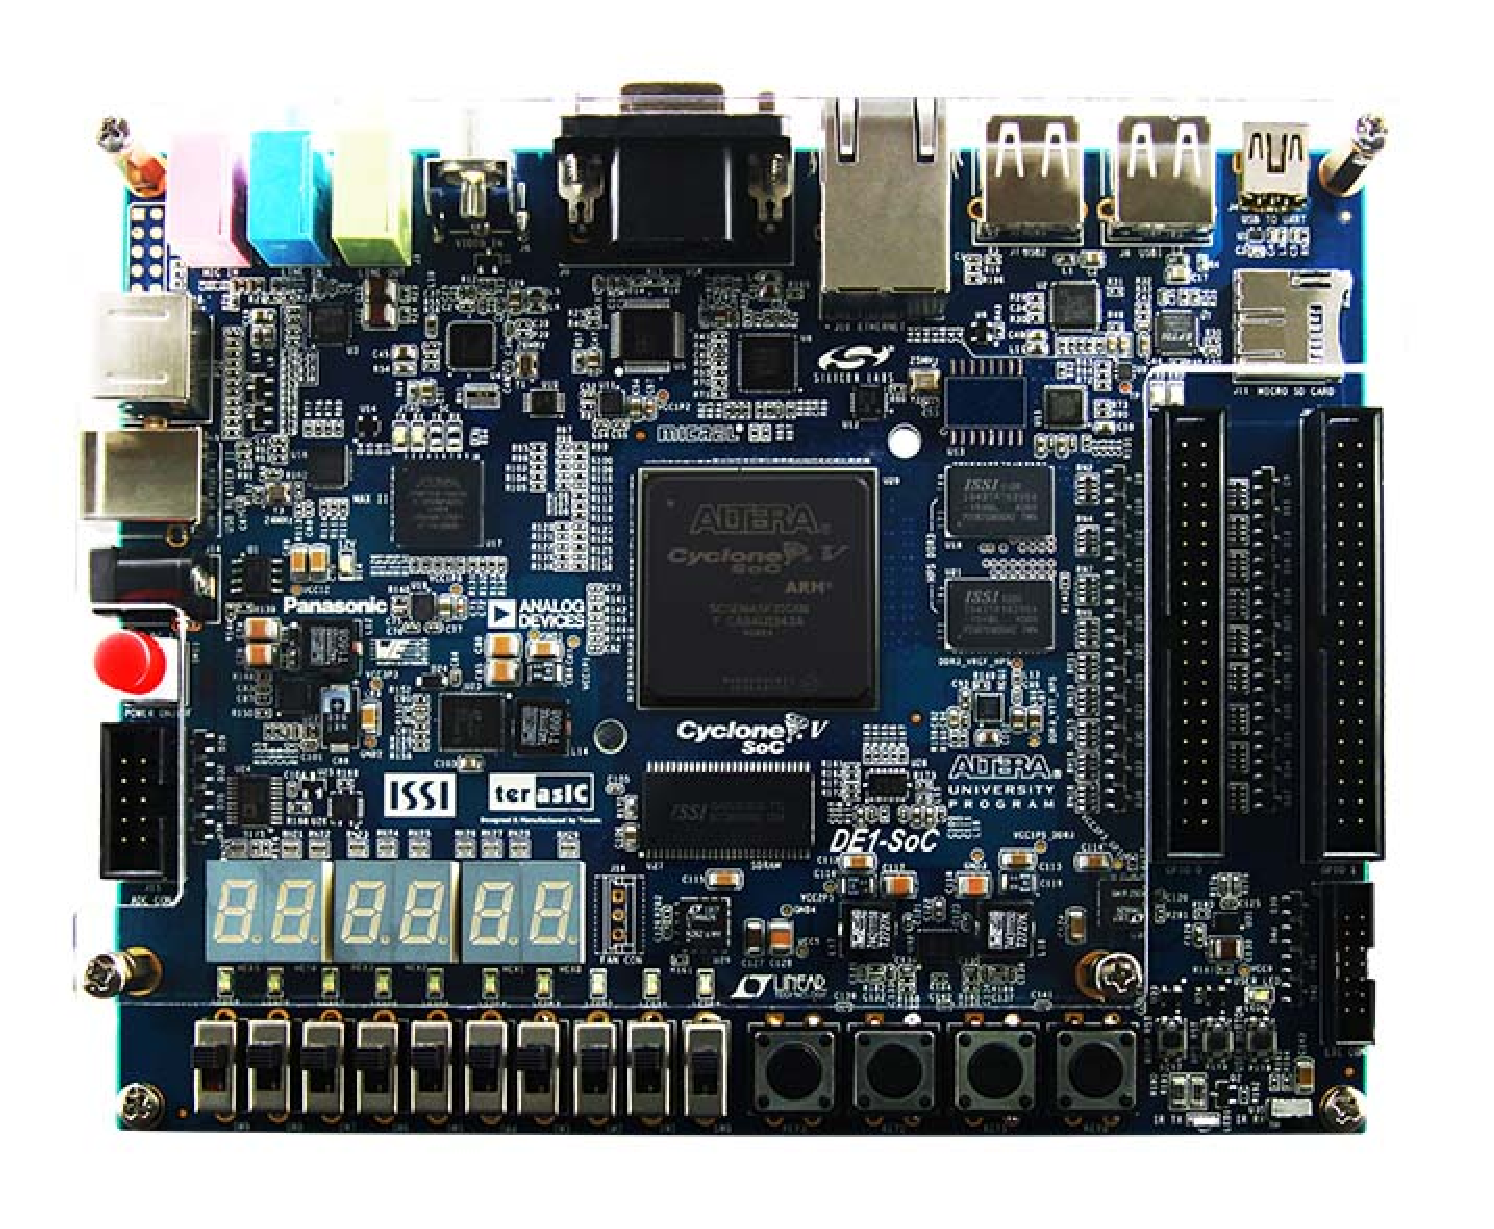
\includegraphics[scale=0.5]{eps/DE1SoC.eps}
\vskip 0.1in
\end{center}

\begin{center}
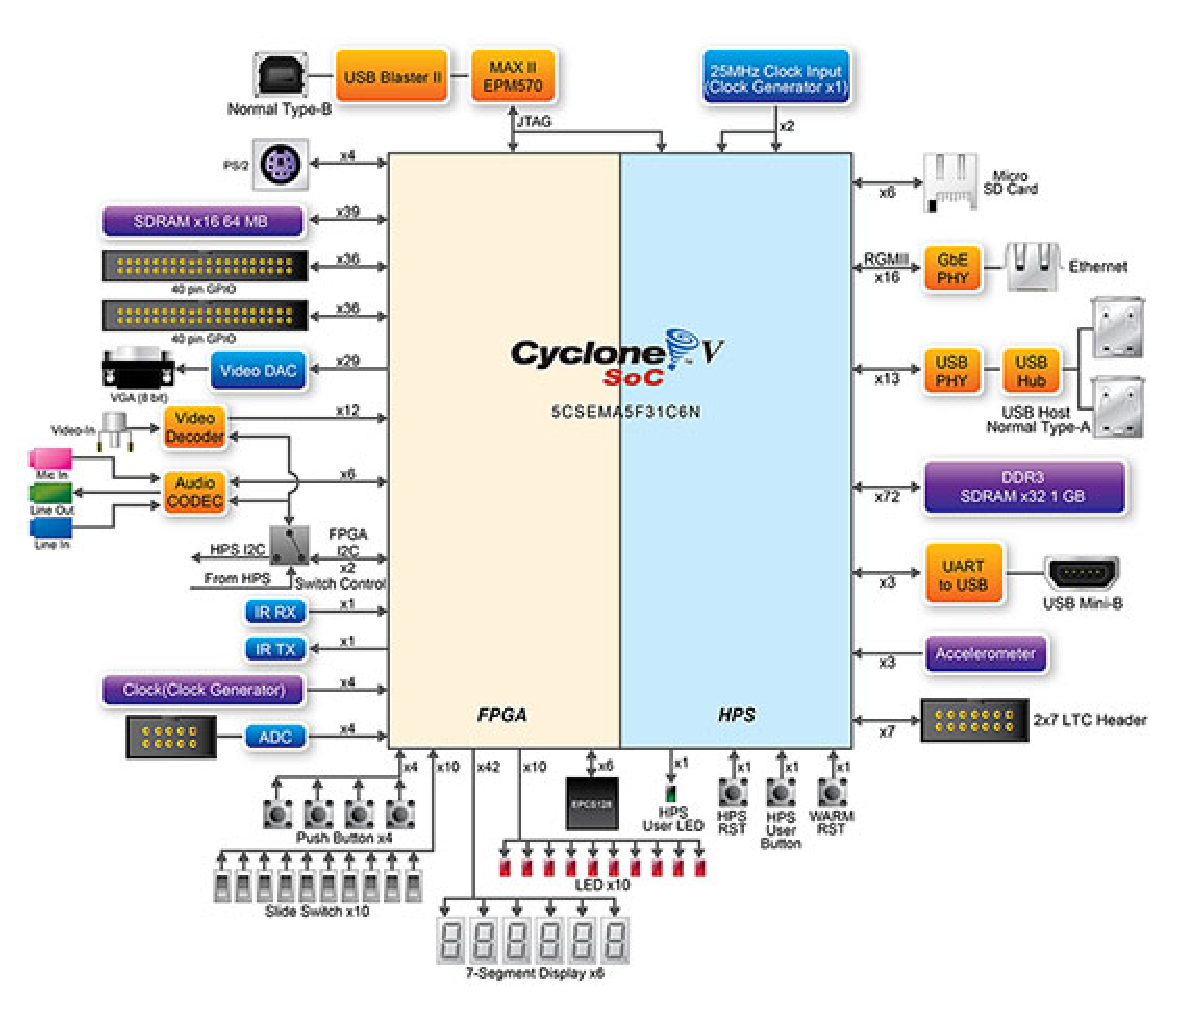
\includegraphics[scale=0.75]{eps/DE1SoCports.eps}
\vskip 0.1in
\end{center}

\section{FPGA Background}
\begin{itemize}
\item {\bf First Use}
\url{http://wl.altera.com/customertraining/webex/Begin_Simple_FPGA_Design/presentation.html}
\item Hardware-Based Packet Filtering Using FPGAs\cite{25}
\item Design of a Embedded Ethernet Packet Sniffer\cite{26}
\end{itemize}

\section{DE1-SoC Setup}
The Quartus II software package needs to be installed.

The DE1 board communicates using COM3 @ 115200/8/1 baud rate, no parity.

The board runs a linux operating system image from a micro-SD card.
The only login is root with no password.




\subsection{Hardware Tradeoff Matrix\cite{4}}
\begin{tabular}{llllll}
         &x86&GPU&DSP&FPGA&$\mu{}$C\\
embed   &maybe &hard      &easy      &easy&easy\\
low power&unusual &nope  &sometimes &sometimes &yes\\
float op&good&excellent&excellent&possible&nope\\
int op&excellent&excellent&excellent&excellent&mediocore\\
control flow&excellent&challenging&air&challenging&excellent\\
io&mediocore&nope&ok&ginormous&ok\\
pipelining&nope&nope&nope&yes&nope\\
programmable&easy&medium&medius&challenging&easy\\
timing control&medium&what?&fair&excellent&fair\\
\end{tabular}

state machines / random numbers 
PSHDL / myHDL / Verilog / VHDL

Xilinx / Altera / Actel (microsem) / Lattice

Ethernet hardware chip
news.thomasnet.com/fullstory/hardwired-tcp-ip-ic-offloads-stack-for-high-speed-internet-490029

\subsection{FPGA Development Boards\cite{4}}
\begin{tabular}{llll}
& actel&altera&xilinx\\
cheap&PSHDL board&DE0-Nano&Papilo One (Spartan 3)\\
&&bemicro CV&mojo Vs (spartan 6)\\
&&&XuLA2-LX25\\
powerful&igloo 2 boards&cyclone 5/arria&artix/kintex/virtex\\
SoC&smartfusion2 starter kit&EBV SoCrates&MicroZedBoard\\
&SmartFusion Starter kit&&parallella\\
CPU+FPGA&Daenkrake&&Logi\\
\end{tabular}

deny by default

disaster recovery


stealing backups
recovery plan

software
  user-mode
  kernel-mode
  hypervisor
  firmware
  microcode
  hardware
  physics

hardware exfilt:
  http://es.slideshare.net/ortegaalfredo/deep-submicronbackdoorsortegasyscan2014slides
    modify chip to detect sequence
    toggle hardware line (e.g. led) to generate radio freq
    listen with radio

infilltration

size of information

  key is easy... use blinds

  database is hard ... large volume

cloud?

sysadmin attacks (snowden/anthem)

fpga/asic

runtime reconfigurable systems

\url{http://media.ccc.de/browse/congress/2013/30C3_-_5443_-_en_-_saal_g_201312281830_-_introduction_to_processor_design_-_byterazor.html#video&t=370}

\url{http://byterazor.federationhq.de/download/handout_30C3.pdf}

fpga 50 dollars

  serial cable

  logic analyzer

  VHDL / Verilog

\url{http://tama-www.informatik.uni-hamburg.ed/vhdl/doc/cookbook/VHDL-Cookbook.pdf}

www.altera.com 6Gbps (starter kit)

regular, random machine audits (aka drug policy)

work from home?

Ring-level security policy?

finding out (e.g. watermarks, RFID tags)

dual computer policy? (plugged USB/secure only networking/loctite screws)

\begin{quote}
"Many businesses erro by putting too much faith in technology alone,
or by starting a security program with a technology blitz. The best
security technology in the world won't produce a good return on
investment without the foundation of security processes, policies, and
education. Instead, businesses should start by evaluating employee
behavior and the associated risks based on factors such as the locale
and the threat landscape. Then treat education, security training, and
business processes can be scuplted around that intelligence. At that
point, appropriate investments in security technology can be applied"
\cite{2}
\end{quote}

outsiders let inside

  "cleaner attacks"/"copier attacks"/"video stream encrypt"

BYOD

mobility

cloud

internet

wifi

USB

unauthorized software

email

provisioning

privileged account management

managing access


\chapter{Sha1 VHDL code \cite{44}}
\begin{chunk}{sha1.v}
/////////////////////////////////////////////////////////////////////
////                                                             ////
////  SHA-160                                                    ////
////  Secure Hash Algorithm (SHA-160)                            ////
////                                                             ////
////  Author: marsgod                                            ////
////          marsgod@opencores.org                              ////
////                                                             ////
////                                                             ////
////  Downloaded from: http://www.opencores.org/cores/sha_core/  ////
////                                                             ////
/////////////////////////////////////////////////////////////////////
////                                                             ////
//// Copyright (C) 2002-2004 marsgod                             ////
////                         marsgod@opencores.org               ////
////                                                             ////
////                                                             ////
//// This source file may be used and distributed without        ////
//// restriction provided that this copyright statement is not   ////
//// removed from the file and that any derivative work contains ////
//// the original copyright notice and the associated disclaimer.////
////                                                             ////
////     THIS SOFTWARE IS PROVIDED ``AS IS'' AND WITHOUT ANY     ////
//// EXPRESS OR IMPLIED WARRANTIES, INCLUDING, BUT NOT LIMITED   ////
//// TO, THE IMPLIED WARRANTIES OF MERCHANTABILITY AND FITNESS   ////
//// FOR A PARTICULAR PURPOSE. IN NO EVENT SHALL THE AUTHOR      ////
//// OR CONTRIBUTORS BE LIABLE FOR ANY DIRECT, INDIRECT,         ////
//// INCIDENTAL, SPECIAL, EXEMPLARY, OR CONSEQUENTIAL DAMAGES    ////
//// (INCLUDING, BUT NOT LIMITED TO, PROCUREMENT OF SUBSTITUTE   ////
//// GOODS OR SERVICES; LOSS OF USE, DATA, OR PROFITS; OR        ////
//// BUSINESS INTERRUPTION) HOWEVER CAUSED AND ON ANY THEORY OF  ////
//// LIABILITY, WHETHER IN  CONTRACT, STRICT LIABILITY, OR TORT  ////
//// (INCLUDING NEGLIGENCE OR OTHERWISE) ARISING IN ANY WAY OUT  ////
//// OF THE USE OF THIS SOFTWARE, EVEN IF ADVISED OF THE         ////
//// POSSIBILITY OF SUCH DAMAGE.                                 ////
////                                                             ////
/////////////////////////////////////////////////////////////////////

`define SHA1_H0 32'h67452301
`define SHA1_H1 32'hefcdab89
`define SHA1_H2 32'h98badcfe
`define SHA1_H3 32'h10325476
`define SHA1_H4 32'hc3d2e1f0

`define SHA1_K0 32'h5a827999
`define SHA1_K1 32'h6ed9eba1
`define SHA1_K2 32'h8f1bbcdc
`define SHA1_K3 32'hca62c1d6

module sha1 (clk_i, rst_i, text_i, text_o, cmd_i, cmd_w_i, cmd_o);
  input    clk_i;   // global clock input
  input    rst_i;   // global reset input , active high
  
  input  [31:0]  text_i;  // text input 32bit
  output  [31:0]  text_o;  // text output 32bit
  
  input  [2:0]  cmd_i;  // command input
  input    cmd_w_i;// command input write enable
  output  [3:0]  cmd_o;  // command output(status)

  /*
    cmd
    Busy Round W R

    bit3 bit2  bit1 bit0
    Busy Round W    R
    
    Busy:
    0  idle
    1  busy
    
    Round:
    0  first round
    1  internal round
    
    W:
    0       No-op
    1  write data
    
    R:
    0  No-op
    1  read data
      
  */
  

      reg  [3:0]  cmd;
      wire  [3:0]  cmd_o;
      
      reg  [31:0]  text_o;
      
      reg  [6:0]  round;
      wire  [6:0]  round_plus_1;
      
      reg  [2:0]  read_counter;
      
      reg  [31:0]  H0,H1,H2,H3,H4;
      reg  [31:0]  W0,W1,W2,W3,W4,W5,W6,W7,W8,W9,W10,W11,W12,W13,W14;
      reg  [31:0]  Wt,Kt;
      reg  [31:0]  A,B,C,D,E;

      reg    busy;
      
      assign cmd_o = cmd;
      always @ (posedge clk_i)
      begin
        if (rst_i)
          cmd <= 'b0;
        else
        if (cmd_w_i)
          cmd[2:0] <= cmd_i[2:0];    // busy bit can't write
        else
        begin
          cmd[3] <= busy;      // update busy bit
          if (~busy)
            cmd[1:0] <= 2'b00;  // hardware auto clean R/W bits
        end
      end
      
      // Hash functions
  wire [31:0] SHA1_f1_BCD,SHA1_f2_BCD,SHA1_f3_BCD,SHA1_Wt_1;
  wire [31:0] SHA1_ft_BCD;
  wire [31:0] next_Wt,next_A,next_C;
  wire [159:0] SHA1_result;
  
  assign SHA1_f1_BCD = (B & C) ^ (~B & D);
  assign SHA1_f2_BCD = B ^ C ^ D;
  assign SHA1_f3_BCD = (B & C) ^ (C & D) ^ (B & D);
  
  assign SHA1_ft_BCD = (round < 'd21) ? SHA1_f1_BCD : (round < 'd41) ? SHA1_f2_BCD : (round < 'd61) ? SHA1_f3_BCD : SHA1_f2_BCD;
  
      assign SHA1_Wt_1 = {W13 ^ W8 ^ W2 ^ W0};

  assign next_Wt = {SHA1_Wt_1[30:0],SHA1_Wt_1[31]};  // NSA fix added
  assign next_A = {A[26:0],A[31:27]} + SHA1_ft_BCD + E + Kt + Wt;
  assign next_C = {B[1:0],B[31:2]};
  
  assign SHA1_result   = {A,B,C,D,E};
  
  assign round_plus_1 = round + 1;
  
  //------------------------------------------------------------------  
  // SHA round
  //------------------------------------------------------------------
  always @(posedge clk_i)
  begin
    if (rst_i)
    begin
      round <= 'd0;
      busy <= 'b0;

      W0  <= 'b0;
      W1  <= 'b0;
      W2  <= 'b0;
      W3  <= 'b0;
      W4  <= 'b0;
      W5  <= 'b0;
      W6  <= 'b0;
      W7  <= 'b0;
      W8  <= 'b0;
      W9  <= 'b0;
      W10 <= 'b0;
      W11 <= 'b0;
      W12 <= 'b0;
      W13 <= 'b0;
      W14 <= 'b0;
      Wt  <= 'b0;
      
      A <= 'b0;
      B <= 'b0;
      C <= 'b0;
      D <= 'b0;
      E <= 'b0;
      
      H0 <= 'b0;
      H1 <= 'b0;
      H2 <= 'b0;
      H3 <= 'b0;
      H4 <= 'b0;

    end
    else
    begin
      case (round)
      
      'd0:
        begin
          if (cmd[1])
          begin
            W0 <= text_i;
            Wt <= text_i;
            busy <= 'b1;
            round <= round_plus_1;
                                                 
            case (cmd[2])
              1'b0:  // sha-1 first message
                begin
                  A <= `SHA1_H0;
                  B <= `SHA1_H1;
                  C <= `SHA1_H2;
                  D <= `SHA1_H3;
                  E <= `SHA1_H4;
                  
                  H0 <= `SHA1_H0;
                  H1 <= `SHA1_H1;
                  H2 <= `SHA1_H2;
                  H3 <= `SHA1_H3;
                  H4 <= `SHA1_H4;
                end
              1'b1:  // sha-1 internal message
                begin
                  H0 <= A;
                  H1 <= B;
                  H2 <= C;
                  H3 <= D;
                  H4 <= E;
                end
            endcase
          end
          else
          begin  // IDLE
            round <= 'd0;
          end
        end
      'd1:
        begin
          W1 <= text_i;
          Wt <= text_i;
          
          E <= D;
          D <= C;
          C <= next_C;
          B <= A;
          A <= next_A;
            
          round <= round_plus_1;
        end
      'd2:
        begin
          W2 <= text_i;
          Wt <= text_i;
          
          E <= D;
          D <= C;
          C <= next_C;
          B <= A;
          A <= next_A;
            
          round <= round_plus_1;
        end
      'd3:
        begin
          W3 <= text_i;
          Wt <= text_i;
          
          E <= D;
          D <= C;
          C <= next_C;
          B <= A;
          A <= next_A;
            
          round <= round_plus_1;
        end
      'd4:
        begin
          W4 <= text_i;
          Wt <= text_i;
          
          E <= D;
          D <= C;
          C <= next_C;
          B <= A;
          A <= next_A;
            
          round <= round_plus_1;
        end
      'd5:
        begin
          W5 <= text_i;
          Wt <= text_i;
          
          E <= D;
          D <= C;
          C <= next_C;
          B <= A;
          A <= next_A;
            
          round <= round_plus_1;
        end
      'd6:
        begin
          W6 <= text_i;
          Wt <= text_i;
          
          E <= D;
          D <= C;
          C <= next_C;
          B <= A;
          A <= next_A;
            
          round <= round_plus_1;
        end
      'd7:
        begin
          W7 <= text_i;
          Wt <= text_i;
          
          E <= D;
          D <= C;
          C <= next_C;
          B <= A;
          A <= next_A;
            
          round <= round_plus_1;
        end
      'd8:
        begin
          W8 <= text_i;
          Wt <= text_i;
          
          E <= D;
          D <= C;
          C <= next_C;
          B <= A;
          A <= next_A;
            
          round <= round_plus_1;
        end
      'd9:
        begin
          W9 <= text_i;
          Wt <= text_i;
          
          E <= D;
          D <= C;
          C <= next_C;
          B <= A;
          A <= next_A;
            
          round <= round_plus_1;
        end
      'd10:
        begin
          W10 <= text_i;
          Wt <= text_i;
          
          E <= D;
          D <= C;
          C <= next_C;
          B <= A;
          A <= next_A;
            
          round <= round_plus_1;
        end
      'd11:
        begin
          W11 <= text_i;
          Wt <= text_i;
          
          E <= D;
          D <= C;
          C <= next_C;
          B <= A;
          A <= next_A;
            
          round <= round_plus_1;
        end
      'd12:
        begin
          W12 <= text_i;
          Wt <= text_i;
          
          E <= D;
          D <= C;
          C <= next_C;
          B <= A;
          A <= next_A;
            
          round <= round_plus_1;
        end
      'd13:
        begin
          W13 <= text_i;
          Wt <= text_i;
          
          E <= D;
          D <= C;
          C <= next_C;
          B <= A;
          A <= next_A;
            
          round <= round_plus_1;
        end
      'd14:
        begin
          W14 <= text_i;
          Wt <= text_i;
          
          E <= D;
          D <= C;
          C <= next_C;
          B <= A;
          A <= next_A;
            
          round <= round_plus_1;
        end
      'd15:
        begin
          Wt <= text_i;
          
          E <= D;
          D <= C;
          C <= next_C;
          B <= A;
          A <= next_A;
            
          round <= round_plus_1;
        end
      'd16,
      'd17,
      'd18,
      'd19,
      'd20,
      'd21,
      'd22,
      'd23,
      'd24,
      'd25,
      'd26,
      'd27,
      'd28,
      'd29,
      'd30,
      'd31,
      'd32,
      'd33,
      'd34,
      'd35,
      'd36,
      'd37,
      'd38,
      'd39,
      'd40,
      'd41,
      'd42,
      'd43,
      'd44,
      'd45,
      'd46,
      'd47,
      'd48,
      'd49,
      'd50,
      'd51,
      'd52,
      'd53,
      'd54,
      'd55,
      'd56,
      'd57,
      'd58,
      'd59,
      'd60,
      'd61,
      'd62,
      'd63,
      'd64,
      'd65,
      'd66,
      'd67,
      'd68,
      'd69,
      'd70,
      'd71,
      'd72,
      'd73,
      'd74,
      'd75,
      'd76,
      'd77,
      'd78,
      'd79:
        begin
          W0  <= W1;
          W1  <= W2;
          W2  <= W3;
          W3  <= W4;
          W4  <= W5;
          W5  <= W6;
          W6  <= W7;
          W7  <= W8;
          W8  <= W9;
          W9  <= W10;
          W10 <= W11;
          W11 <= W12;
          W12 <= W13;
          W13 <= W14;
          W14 <= Wt;
          Wt  <= next_Wt;
          
          E <= D;
          D <= C;
          C <= next_C;
          B <= A;
          A <= next_A;
            
          round <= round_plus_1;
        end
      'd80:
        begin
          A <= next_A + H0;
          B <= A + H1;
          C <= next_C + H2;
          D <= C + H3;
          E <= D + H4;
          round <= 'd0;
          busy <= 'b0;
        end
      default:
        begin
          round <= 'd0;
          busy <= 'b0;
        end
      endcase
    end  
  end 
  
  
  //------------------------------------------------------------------  
  // Kt generator
  //------------------------------------------------------------------  
  always @ (posedge clk_i)
  begin
    if (rst_i)
    begin
      Kt <= 'b0;
    end
    else
    begin
      if (round < 'd20)
        Kt <= `SHA1_K0;
      else
      if (round < 'd40)
        Kt <= `SHA1_K1;
      else
      if (round < 'd60)
        Kt <= `SHA1_K2;
      else
        Kt <= `SHA1_K3;
    end
  end

  //------------------------------------------------------------------  
  // read result 
  //------------------------------------------------------------------  
  always @ (posedge clk_i)
  begin
    if (rst_i)
    begin
      text_o <= 'b0;
      read_counter <= 'b0;
    end
    else
    begin
      if (cmd[0])
      begin
        read_counter <= 'd4;  // sha-1   160/32=5
      end
      else
      begin
      if (~busy)
      begin
        case (read_counter)
          'd4:  text_o <= SHA1_result[5*32-1:4*32];
          'd3:  text_o <= SHA1_result[4*32-1:3*32];
          'd2:  text_o <= SHA1_result[3*32-1:2*32];
          'd1:  text_o <= SHA1_result[2*32-1:1*32];
          'd0:  text_o <= SHA1_result[1*32-1:0*32];
          default:text_o <= 'b0;
        endcase
        if (|read_counter)
          read_counter <= read_counter - 'd1;
      end
      else
      begin
        text_o <= 'b0;
      end
      end
    end
  end
  
endmodule
 
\end{chunk}

\chapter{Sha1 Forth code \cite{30}}

Forth requires words to be defined before they are used so the 
development of a SHA1 program is naturally bottom-up. But we tend
to understand tasks top-down. We use literate programming to support this.

\section{Things to know}
A Forth string is implementation dependent but has been traditionally
represented as a 1-byte count followed by up to 255 bytes of string.
\begin{verbatim}

  +-------+------+------+------+------+-----+-----+
  + count | byte | byte | byte | .... | byte| byte| 
  +-------+------+------+------+------+-----+-----+

\end{verbatim}

Blocks in the SHA algorithm are 512-bit strings, or 64 bytes.

SHA1 operates on 32-bit ``words''. Forth defines operations by defining
``words''. These concepts have nothing to do with each other. 

The SHA algorithm is described using 32-bit words but the J1 cpu is
a 16-bit implementation so we need to define some primitive words that
operate on the data in 32-bit words. In particular, the SHA1 algorithm
defines operations on words (section 3 of the standard) as:
\begin{verbatim}
Bitwise logical word operations

   X AND Y = bitwise logical "and" of X and Y.
   X OR Y  = bitwise logical "inclusive-or" of X and Y.
   X XOR Y = bitwise logical "exclusive-or" of X and Y.
   NOT Y   = bitwise logical "complement" of X.
\end{verbatim}

The words {\bf rot}, {\bf -rot}, {\bf OR}, {\bf XOR}, {\bf AND}, {\bf swap}
are standard Forth words defined as:
\begin{verbatim}
 rot ( x1 x2 x3 -- x2 x3 x1 )
-rot ( x1 x2 x3 -- x3 x1 x3 )
 or  ( x1 x2 -- x )
xor  ( x1 x2 -- x )
and  ( x1 x2 -- x )
swap ( x1 x2 -- x2 x1 )
\end{verbatim}

The Forth ``double'' implementation of these are
\begin{chunk}{logicalops}
\ Double versions of bitwise and, or, xor
 
: DOR ( d1 d2 -- d3 )
  rot OR -rot OR swap ;
: DXOR ( d1 d2 -- d3 )
  rot XOR -rot XOR swap ;
: DAND ( d1 d2 -- d3 ) 
  rot AND -rot AND swap ;
  
\end{chunk}

In order to understand how these words work you need to know that
{\bf d1} and {\bf d2} are ``double'' (32-bit) words. This means that they are
stored on the stack as 2 ``single'' (16-bit) words. So if we look at a
stack trace of the operations of {\bf DOR} we would see:
\begin{verbatim}
initial:  d1hi d1lo d2hi d2lo
    rot:  d1hi d2hi d2lo d1lo
     OR:  d1hi d2hi dlo
   -rot:  dlo  d1hi d2hi
     OR:  dlo  dhi
   swap:  dhi  dlo
\end{verbatim}

\section{The SHA1 standard \cite{30}}
\subsection{Message Padding}

The purpose of message padding is to make the total length of a padded
message a multiple of 512 bits. SHA1 sequentially processes blocks of
512 bits when computing the message digest. The following specifies
how this padding shall be performed. As a summary, a ``1'' followed by
m ``0''s followed by a 64-bit integer are appended to the end of the
message to produce a padded message of length 512 * n. The 64-bit
integer is the length of the original message. The padded message is then
processed by the SHA1 as n 512-bit blocks.

Suppose a message has length L $< 2^{64}$. Before it is input to the
SHA1, the message is padded on the right as follows:
\begin{enumerate}[a.]
\item ``1'' is appended. Example: if the original message is ``01010000'',
this is padded to ``010100001''.
\item ``0''s are appended. The number of ``0''s will depend on the
original length of the message. The last 64 bits of the last 512-bit
block are reserved for the length L of the original message.\\
Example: Suppose the original message is the bit string
\begin{verbatim}
  01100001 01100010 01100011 01100100 01100101
\end{verbatim}
After step (a) this gives
\begin{verbatim}
  01100001 01100010 01100011 01100100 01100101 1
\end{verbatim}
Since L = 40, the number of bits in the above is 41 and 407 ``0''s are
appended, making the total now 448. This gives (in hex)
\begin{verbatim}
  61626364 65800000 00000000 00000000
  00000000 00000000 00000000 00000000
  00000000 00000000 00000000 00000000
  00000000 00000000 
\end{verbatim}
\item Obtain the 2-word representation of L, the number of bits in the
original message.\\
If L $< 2^{32}$ then the first word is all zeros. Append
these two words to the padded message.\\
Example: Suppose the original message is as in (b). Then L = 40 (note that
L is computed before any padding). The two-word representation of 40 is
hex \verb|00000000 00000028|. Hence the final padded message in hex is
\begin{verbatim}
  61626364 65800000 00000000 00000000
  00000000 00000000 00000000 00000000
  00000000 00000000 00000000 00000000
  00000000 00000000 00000000 00000028
\end{verbatim}
The padded message will contain 16 * $n$ words for some $n > 0$. 
The padded message is regarded as a sequence of $n$ blocks M(1),
M(2), first characters (or bits) of the message.
\end{enumerate}

Note that this implementation assumes that the message is already
properly padded.

\subsection{Functions and Constants used}

A sequence of logical functions $f(0)$, $f(1)$, ..., $f(79)$ is used in
SHA1. Each $f(t)$, $0 \le t \le 79$, operates on 32-bit words B, C, D,
and produces a 32-bit word as output. $f(t;B,C,D)$ is defined as follows:
\begin{verbatim}
   f(t;B,C,D) = (B AND C) OR ((NOT B) AND D)       (  0 <= t <= 19 )
   f(t;B,C,D) = B XOR C XOR D                      ( 20 <= t <= 39 )
   f(t;B,C,D) = (B AND C) OR (B AND D) OR (C AND ) ( 40 <= t <= 59 )
   f(t;B,C,D) = B XOR C XOR D                      ( 60 <= t <= 79 )
\end{verbatim}

These are actually 3 distinct functions, defined in Forth as
\begin{chunk}{logicalfns}
: __F                 ( dd dc db -- bc or b'd )
    2DUP D>R DAND 2SWAP DR> DINVERT DAND DOR ;

: __G                 ( d c b -- bc or bd or cd )
    4DUP DAND D>R  DOR DAND DR>  DOR ;

: __H                 ( d c b -- d xor c xor b )
    DXOR DXOR ;

\end{chunk}

A sequence of constant words $K(0)$, $K(1)$, ... $K(79)$ is used in
SHA1. In hex these are given by
\begin{verbatim}
  K(t) = 5A827999    (  0 <= t <= 19 )
  K(t) = 6ED9EBA1    ( 20 <= t <= 39 )
  K(t) = 8F1BBCDC    ( 40 <= t <= 59 )
  K(t) = CA62C1D6    ( 60 <= t <= 79 )
\end{verbatim}
The implementation uses these as explicit constants 
in the {\bf transform} word which will be explained later.

\subsection{Computing the message digest}
Before processing any blocks, the H's are initialized as follows (in hex)
\begin{verbatim}
  H0 = 67452301
  H1 = EFCDAB89
  H2 = 98BADCFE
  H3 = 10325476
  H4 = C3D2E1F0
\end{verbatim}
These are set up as explicit contants used in {\bf sha-init}, described
below.

\section{Forth Implementation}
\subsection{Storage}
{\bf SIZE} is a ``double'' location

So we create a {\bf SIZE} ``double'' variable and a {\bf Single-Bytee} 
variable.
\begin{chunk}{SIZE}
2VARIABLE SIZE
VARIABLE Single-Bytee

\end{chunk}

The name {\bf Message-Digest} is a constant pointer to a memory location
of 5 32-bit cells to hold the 160 bit SHA1 hash result.
\begin{chunk}{Message-Digest}
\ Source program uses: CREATE Message-Digest   5 CELLS ALLOT
VHERE 5 CELLS VALLOT
XCONSTANT Message-Digest

\end{chunk}

\subsection{sha1}
The top level word {\bf sha1} expects the address of a Forth string.

The {\bf sha1} function expects the address of a string at the top of stack.
It returns the SHA1 sum of the string.

It calls {\bf sha-init} for initialization. This will set up the initial
bytes in {\bf Message-Digest} to seed the algorithm. It has no final 
effect on the stack so the initial address argument to {\bf sha1} is
the top of stack.

We compute the count which computes ( addr1 -- addr2 n ) where $n$ is the
length of the string at addr1 and addr2 points to the first byte. The
word {\bf \verb|u>d|} extends the length $n$ to be a double so the 
stack now looks like 
\begin{verbatim}
  ( first-byte-of-string n 0 -- )
\end{verbatim}
We then call {\bf sha-update} to compute the SHA1.

It calls {\bf sha-final} to clean up after itself.

It calls {\bf .sha} to print the final result.

\begin{chunk}{sha1}
\ top level word
: sha1 ( string-xaddress )
  sha-init
  count u>d sha-update
  sha-final
.sha ;

\end{chunk}

\subsection{sha-init}
This puts the {\bf Message-Digest} address on the stack, pushes
SHA1 constants onto the stack, and stores them into memory. So
memory at {\bf Message-Digest} now contains the 160-bit constant
(in hex):
\begin{verbatim}
67 45 23 01 EF CD AB 89 98 BA DC FE 10 32 54 76 C3 D2 E1 F0
\end{verbatim}
and the memory locate {\bf SIZE} is set to (in hex)
\begin{verbatim}
00 00
\end{verbatim}

\begin{chunk}{sha-init}
: SHA-INIT          ( -- )
    \  Initialize Message-Digest with starting constants.
    Message-Digest
        din 0x67452301 2OVER 2! CELL xn+
        din 0xEFCDAB89 2OVER 2! CELL xn+
        din 0x98BADCFE 2OVER 2! CELL xn+
        din 0x10325476 2OVER 2! CELL xn+
        din 0xC3D2E1F0 2SWAP 2!
    \  Zero bit count.
    0. SIZE 2! ;

\end{chunk}

\subsection{sha-update}
do for each 
\begin{chunk}{sha-update}
: SHA-UPDATE ( stringxaddr doublelen -- )
   4 needed
                         \ Transform 512-bit blocks of message.
    BEGIN                \ Transform Message-Block?
        size 2@          \ fetch upper cell (4 bytes) of SIZE variable
        0x1ff u>d DAND   \ fast modulo 512
        0x3 DRSHIFT      \ shift result 3 ( for example 511 >> 3 is 63 )
        D>R              \ save to return stack, name: modshiftcount
        0x40 U>D DR@ D-  \ grab from return stack, 64 subtract modshiftcount
        2OVER DU> NOT    \ copy string count compare for loop
        
    WHILE                \ Store some of str&len, and transform. 
                         \ duplicate string and count        
        4DUP                 ( xstr dlen xstr dlen)
                         \ 64 subtract dmodshiftcount 
        0x40 U>D DR@ D-      ( xstr dlen xstr dlen dnewlen)
                         \ convert len,newlen to single width
        drop nip             ( xstr dlen xstr len newlen)
                         \ cut string to newlen
        /STRING              ( xstr dlen xnewstr (len-newlen) )
                         \ duplicate the difference, save to rstack
        U>D 2DUP D>R         ( xstr dlen xnewstr d(len-newlen) )  
        4SWAP                ( xnewstr d(len-newlen) xstr dlen )
                         \ grab difference from rstack, 
                         \ use it to get newlen in top cell
        DR> D-               ( xnewstr d(len-newlen) xstr dnewlen ) 
        Message-Block DR@ D+ ( xnewstr d(len-newlen) xstr 
                             \ dnewlen xmessageaddr+modshiftcount )
        2SWAP                ( xnewstr d(len-newlen) xstr 
                             \ xmessageaddr+modshiftcount dnewlen )
        drop                 ( xnewstr d(len-newlen) xstr 
                             \ xmessageaddr+modshiftcount newlen )
        MOVE                 ( xnewstr d(len-newlen) )
        TRANSFORM            ( xnewstr d(len-newlen) )
        SIZE 2@              ( xnewstr d(len-newlen) dsize ) 
        0x40 U>D DR>         ( xnewstr d(len-newlen) dsize 
                             \  0x40 0 dmodshiftcount)
        D- 
        3 DLSHIFT D+ SIZE 2!  ." in" size 2@ d.
    REPEAT
    \  Save final fraction of input.
                         ( stringxaddr doublelen )
    Message-Block DR> D+ ( stringxaddr doublelen 
                         \ messageblockxaddr+modshiftcount ) 
    2SWAP  2DUP          ( stringxaddr 
                         \ messageblockxaddr+modshiftcount 
                         \ doublelen doublelen )
    D>R                  ( stringxaddr messageblockxaddr+modshiftcount 
                         \ doublelen )
    drop CMOVE  ( )      \ CMOVE
    SIZE 2@ DR>  D2* D2* D2* D+ SIZE 2! ( )
    ;
    
\end{chunk}

\subsection{Fetch-Message-Digest}
This puts 160 bits on the stack
\begin{chunk}{Fetch-Message-Digest}
   : Fetch-Message-Digest   ( -- de dd dc db da )
        4 CELLS U>D Message-Digest D+  ( addr)
            2DUP 2@ 2SWAP CELL U>D d-  ( e addr)
            2DUP 2@ 2SWAP CELL U>D d-  ( e d addr)
            2DUP 2@ 2SWAP CELL U>D d-  ( e d c addr)
            2DUP 2@ 2SWAP CELL U>D d-  ( e d c b addr)
                2@ ;                   ( e d c b a)

\end{chunk}

\subsection{Add-to-Message-Digest}
This adds the 160 bits on the top of the stack to the current SHA1 sum.
\begin{chunk}{Add-to-Message-Digest}
    : Add-to-Message-Digest  ( de dd dc db da -- )
        Message-Digest                 ( e d c b a addr)
            DTUCK 2+! CELL U>D D+      ( e d c b addr)
            DTUCK 2+! CELL U>D D+      ( e d c addr)
            DTUCK 2+! CELL U>D D+      ( e d addr)
            DTUCK 2+! CELL U>D D+      ( e addr)
                 2+! ;                 ( )

\end{chunk}

\subsection{transform}
\begin{chunk}{transform}
: TRANSFORM         ( -- )
    Fetch-Message-Digest    ( e d c b a)

    \  Do 80 Rounds of Complicated Processing.
    0x10  0x0 DO  D>R  6DUP __F din 0x5A827999 D+  DR>  I BLK0  MIX  LOOP
    0x14 0x10 DO  D>R  6DUP __F din 0x5A827999 D+  DR>  I BLK   MIX  LOOP
    0x28 0x14 DO  D>R  6DUP __H din 0x6ED9EBA1 D+  DR>  I BLK   MIX  LOOP
    0x3c 0x28 DO  D>R  6DUP __G din 0x8F1BBCDC D+  DR>  I BLK   MIX  LOOP
    0x50 0x3c DO  D>R  6DUP __H din 0xCA62C1D6 D+  DR>  I BLK   MIX  LOOP

    Add-to-Message-Digest ;

\end{chunk}

\subsection{blk0}
{\bf BLK0} converts the first 16 cells of Message-Block to Work-Block.
{\bf BLK0} takes single-width index i,
which is added to the base of Message-Block and two-fetched
\begin{chunk}{blk0}
: BLK0              ( i -- d )     \  Big Endian
    CELLS Message-Block rot xn+ 2@ ;

\end{chunk}

\subsection{blk}
{\bf BLK} converts the remaining cells of Message-Block to Work-Block. 
{\bf BLK0} takes single-width index i, does some fancy XOR work folding
into the same double. saves the final result to Message-Block,
and also returns it ( final double )
\begin{chunk}{blk}
: BLK               ( i -- d )
    DUP  0xd + 0xf AND CELLS Message-Block rot xn+ 2@
    2 pick 0x8 + 0xf AND CELLS Message-Block rot xn+ 2@  DXOR
    2 pick 0x2 + 0xf AND CELLS Message-Block rot xn+ 2@  DXOR
    2 pick       0xf AND CELLS Message-Block rot xn+ 2@  DXOR
    1 DLROTATE  \  This operation was added for SHA-1.
    2DUP 4 roll 15 AND CELLS Message-Block rot xn+ 2! ;
\end{chunk}

\subsection{mix}
\begin{chunk}{mix}
\  temp = temp + (m + (a <<< 5)) + e
: MIX ( e d c b temp a m -- e d c b a )
    2SWAP 2DUP D>R                   ( e d c b temp m a)( R: a)
    0x5 DLROTATE d+ d+               ( e d c b temp)    ( R: a)
    2SWAP D>R  2SWAP D>R  2SWAP D>R  ( e temp)    ( R: a b c d)
    D+                               ( temp)      ( R: a b c d)
    \  e = d
       DR> 2SWAP                     ( e temp)      ( R: a b c)
    \  d = c
       DR> 2SWAP                     ( e d temp)      ( R: a b)
    \  c = (b <<< 30)
       DR> 0x1e DLROTATE             ( e d temp c)      ( R: a)
       2SWAP                         ( e d c temp)      ( R: a)
    \  b = a
       DR>                           ( e d c temp b)     ( R: )
    \  a = temp
       2SWAP                         ( e d c b a)
    ;

\end{chunk}

\subsection{sha-final}

This allocates 9 bytes called {\bf Final-Count}
\begin{chunk}{Final-Count}
VHERE 9 VALLOT
XCONSTANT Final-Count

\end{chunk}
\begin{chunk}{sha-final}
: SHA-FINAL         ( -- )
    \  Save SIZE for final padding.
    
    \ final-count must be 64 bits, so we use 0 0 sizelow sizehi
    0 0 final-count 2!
    SIZE 2@
    Final-Count 4xn+ 2!

    \  Pad so SIZE is 64 bits less than a multiple of 512.
    Single-Bytee 0x80 2 pick 2 pick C!   ( xsingle-bytee )
    1 u>d SHA-UPDATE
    BEGIN  SIZE 2@ 0x1ff u>d DAND 0x1C0 u>d d= NOT WHILE
        Single-Bytee 0 2 pick 2 pick C!  1 u>d SHA-UPDATE
    REPEAT

    \ final-count is 64 bits (hence length of 8)
    Final-Count 8 u>d SHA-UPDATE
    ;

\end{chunk}

\subsection{sha}
This {\bf sha} word will write the final the SHA1 hash, on
the screen by dumping the 20 bytes (160 bits) 
at location {\bf Messsage-Digest}

\begin{chunk}{sha}
: .SHA
cr
." digest: "
   Message-Digest 0x20 dump  cr \  Display Message-Digest.
;

\end{chunk}

\begin{chunk}{sha1forth.fs}
( SHA-160 Secure Hash Algorithm )

\ Based on code taken from:
\ http://www.forth.org.ru/~mlg/mirror/home.earthlink.net/~neilbawd/sha1.html
\ https://github.com/esromneb/Forth-Sha1-16-bit
\ as modified by Tim Daly

decimal 

\ anew nielsha1

\getchunk{dshift}

\ number of bytes per memory address
4 CONSTANT CELL
: CELLS CELL * ;

\ real number of bytes per memory address
2 CONSTANT QEDCELL

\getchunk{SIZE}
\getchunk{Message-Digest}
20 vallot \ burn space for clean printing using dump

\ Source program uses: CREATE Message-Block   16 CELLS ALLOT
VHERE 16 CELLS VALLOT
XCONSTANT Message-Block

\getchunk{Final-Count}
\getchunk{logicalops}
\getchunk{stackops}
\getchunk{blk0}
\getchunk{blk}
\getchunk{logicalfns}
\getchunk{mix}
\getchunk{Fetch-Message-Digest}
\getchunk{Add-to-Message-Digest}
\getchunk{transform}
\getchunk{sha-init}
\getchunk{sha-update}
\getchunk{sha-final}
\getchunk{sha}
\getchunk{sha1}

hex

\ zero out variable memory.
\ some of this is taken care of in sha-init
2000 0 100 0 fill

\end{chunk}

\section{Forth Word Dictionary}
\subsection{Standard Forth Words}
The standard words mean:
\begin{verbatim}
."                       Write the characters to the terminal until the
                         matching trailing "

/STRING ( addr1 u1 n -- addr2 u2 ) Adjust the string at addr1 u1 by n
                                   characters. Return addr2=addr1+n
                                   with length u2 = u1-n

2! ( x1 x2 addr -- ) Stores two 16-bit words at addr

2@ ( addr -- x1 x2 ) Fetches two 16-bit words at addr

2DUP ( x1 x2 -- x1 x2 x1 x2 ) Dup top 2 cells on stack

2OVER ( x1 x2 x3 x4 -- x1 x2 x3 x4 x1 x2 ) Copy cell pair x1,x2 to stack top

2SWAP ( x1 x2 x3 x4 -- x3 x4 x1 x2 ) Exchange top two cell pairs

2VARIABLE <name> ( - ) Create a dictionary entry for name associated with
                       two cells of data space. Using <name> returns the
                       address of the first cell of the data space on 
                       the stack.

4DUP ( x1 x2 x3 x4 -- x1 x2 x3 x4 x1 x2 x3 x4 ) Dup top 4 cells on stack

4xn+ ( addr1 -- addr2 ) Adds 4 to addr1 yielding addr2

ALLOT ( u -- )           Allocate u bytes of data space beginning 
                         at the next available location.

CELL is the "word size" of the machine (2 bytes in this case)

CELLS ( n1 -- n2 )       Returns n2, the size in bytes of n1 cells

CONSTANT <name> ( x -- ) Create a dictionary entry for name 
                         associated with value x

count ( addr1 -- addr2 u ) Returns the length u and the address of the
                           text portion of the string at addr1

cr                       Write a newline to the terminal

D- ( d1 d2 -- d3 ) Subtracts two signed double

D+ ( d1 d2 -- d3 ) Adds two signed double

D>R ( d -- ) (R: -- d ) move a double from the stack to the return stack

DO ( n1 n2 - ) Establish the loop parameters. This word expects the
               initial loop index n2 on top o the stack, with the
               limit value n1 beneath it. These values are removed
               from the stack and stored elsewhere, usually on the
               return stack, when DO is executed. 

DU> ( ud1 ud2 -- flag ) Flag is TRUE if the unsigned double ud1 is greater
                        than the unsigned double ud2.

DR@ ( -- d ) (R: d -- d ) Copies the top double number on the return stack
                          to the data stack

DROP ( w -- ) Drops top cell off stack

din ( -- wd ) DIN removes the next word from the input stream, converts
              it to a 32-bit double number wd in the current base, and
              executes 2literal which leaves the number on the stack. So
              HEX DIN 12345678 ( -- 5678 1234 )

DRSHIFT ( xhi xlo u -- xhi2 xlo2 ) Shift the double u bits right

DUMP ( addr +n -- )      Display the contents o a memory region of length +n
                         starting at address addr

HERE ( - addr )          Push the address of the next available location 
                         in data space onto the stack

MOVE ( addr1 addr2 u -- ) Copy u bytes at addr1 to the destination addr2

NIP ( x1 x2 -- x2 ) Drops the cell below the top of stack

pick ( +n -- x ) Place a copy of the nth entry on top of stack
                 This is 0-based so 0 pick is dup, 1 pick is over

u>d ( u -- d ) Converts an unsigned number to double on the stack
               Its definition is 
   0 constant u>d

VARIABLE <name> ( - )  Create a dictionary entry for name associated with
                       one cell of data space. Using <name> returns the
                       address of the cell of the data space on the stack.

xn+ ( addr1 n -- addr2 ) adds signed integer n to addr1 to get addr2

\end{verbatim}

\subsection{Locally defined Forth words}
These words have been defined specifically for this algorithm.
\begin{chunk}{stackops}
\DTUCK ( d1h1 d1lo d2hi d2low -- d2hi d2lo d1hi d1lo d2hi d2low )
\                         Place a copy of the double below the second
\                         double on the stack.
: DTUCK 2swap 2over ; 

\6DUP ( x1 x2 x3 x4 x5 x6 -- x1 x2 x3 x4 x5 x6 x1 x2 x3 x4 x5 x6 ) 
\            Dup top 6 cells on stack
: 6DUP 4 xpick 4 xpick 4 xpick ;

\4SWAP ( x1 x2 x3 x4 x5 x6 x7 x8 -- x5 x6 x7 x8 x1 x2 x3 x4 ) 
\                        Exchange top 4 cell pairs
: 4SWAP 7 roll 7 roll 7 roll 7 roll ;

\ \\ this is the equivalent of +! 
\ \\ : +! 2dup @ 3 pick + -rot ! drop ;
\ two-plus-store
: 2+! 2dup 2@ 4 xpick d+ 2swap 2! 2drop ;

: DLSHIFT DSHIFT ;
: DRSHIFT negate DSHIFT ;

: INVERT complement ;

: DINVERT complement swap complement swap ;

: DLROTATE           ( d1 n -- d2 )
    3DUP  DLSHIFT D>R  32 SWAP -  DRSHIFT DR>  DOR ;

hex
: LROTATE           ( x n -- x' )
  0 swap dlshift or ;

: Flip-Endian       ( 0102 -- 0201 )
    DUP 8 LROTATE 0xFF00 AND
    SWAP 8 LROTATE 0x00FF AND OR ;
decimal

\end{chunk}

\subsection{dshift}
NOTE:This routine needs to be rewritten for the J1 processor

This is a general purpose shift word in assembly coded for Freescale
HCS12/9S12.  It logically {i.e.,no sign extension} shifts d1 accding
to the value of n2.  If n2 is positive, n1 is shifted left; if n2 is
neg, n1 is shifted right.  The absolute value of n2 determines the 
number of bits of shifting; unchecked error on overflow/underflow
\begin{chunk}{dshift}
CODE DSHIFT    ( d1 n2 -- d3 )
2 IND,Y LDD   \ D <- msword
4 IND,Y LDX   \ X <- lsword
0 IND,Y TST   \ test msbyte of n2; is n2 negative?
MI IF,        \ if n2 is negative, shift right:
    BEGIN,
      LSRA    \ shift right,preserve top bit, bot bit->carry INCORRECT
      RORB    \ rotate right,carry->top bit
      XGDX    \ D <- lsword, X <- msword, cond.codes unaffected
      RORA    \ shift right; carry->top.bit,bot bit->carry
      RORB    \ shift right; carry->top.bit
      XGDX    \ D <- msword, X <- lsword, cond.codes unaffected
      1 IND,Y INC
    GE UNTIL,
ELSE,         \ if n2 is positive, shift left
  1 IND,Y TST
  GT IF,      \ do nothing if index=0
    BEGIN,
      XGDX    \ D <- lsword, X <- msword, cond.codes unaffected
      LSLD    \ shift left,top bit->carry INCORRECT
      XGDX    \ D <- msword, X <- lsword, cond.codes unaffected
      ROLB    \ rotate left,carry->bottom bit
      ROLA    \ rotate left,carry->bottom bit
      1 IND,Y DEC
    LE UNTIL,
  THEN,
THEN,
2 ,+Y STD     ( d1.lsword\d3.msword -- ) \ save msword
2 IND,Y STX   ( -- d3 ) \ save lsword
RTS
END.CODE

\end{chunk}

\subsection{Dictionary of Algorithm Words}
These words are locally defined
\begin{itemize}
\item DOR ( d1 d2 -- d3 ) double bitwise or
\item DXOR ( d1 d2 -- d3 ) double bitwise xor
\item DAND ( d1 d2 -- d3 ) double bitwise and
\item DTUCK double-width tuck
\item 6DUP duplicate 3 double numbers on the stack
\item 4SWAP
\item 2+! two-plus-store
\item DLSHIFT double left shift
\item DRSHIFT double right shift
\item INVERT complement
\item DINVERT double complement
\item DLROTATE ( d1 n -- d2 ) double left rotate
\item LROTATE ( x n -- x' ) left rotate
\item Flip-Endian ( 0102 -- 0201 )
\item BLK0 ( i -- d ) Convert first 16 cells of Message-Block to Work-Block.
\item BLK ( i -- d ) Convert remaining cells of Message-Block to Work-Block. 
\item \verb|__F| ( dd dc db -- bc or b'd )
\item \verb|__G| ( d c b -- bc or bd or cd )
\item \verb|__H| ( d c b -- d xor c xor b )
\item MIX ( e d c b temp a m -- e d c b a ) temp = temp + (m + (a <<< 5)) + e
\item Fetch-Message-Digest ( -- de dd dc db da )
\item Add-to-Message-Digest  ( de dd dc db da -- )
\item TRANSFORM ( -- ) Do 80 Rounds of Complicated Processing.
\item SHA-INIT ( -- ) Initialize Message-Digest with starting constants.
\item SHA-UPDATE ( stringxaddr doublelen -- ) Transform 512-bit blocks of message.
\item SHA-FINAL ( -- )
\item .SHA ( -- ) Print the final SHA1 hash
\item sha1 ( string-xaddress ) top level word
\end{itemize}




\chapter{Microsoft Related Papers}
Abstract from Putnam\cite{15}:

Datacenter workloads demand high computational complexities,
flexibility, power efficiency, and low cost. It is challenging to
improve all of these factos simultaneously. To advance datacenter
capabilities beyond what commodity server designs can provide, we
have designed and built a composable, reconfigurable fabric to
accelerate portions of large-scale software services.
Each instantiation of the fabric consists of a 6x8 2-D torus of
high-end Stratix V FPGAs embedded into a half-rack of 48
machines. One FPGA is placed into each server, accessible through
PCIe, and wired directly to other FPGAs with pairs of 10 Gb SAS
cables.

In this paper, we describe a medium-scale deployment of
this fabric on a bed of 1,632 servers, and measure its efficacy in
accelerating the Bing web search engine. We describe the
requirements and architecture of the system, detail the
critical engineering challenges and solutions needed to make
the system robust in the presence of failures, and measure
the performance, power, and resilence of the system when
ranking candidate documents. Under high load, the
large-scale reconfigurable fabric improves the ranking throughput
of each server by a factor of 95\% for a fixed latency distribution --
or, while maintaining equivalent throughput, reduces the tail 
latency by 29\%.

Abstract from Kim\cite{16}:

Data compression is crucial in large-scale storage servers to save
both storage and network bandwidth, but it suffers from high
computational cost. In this work, we present a high throughput FPGA
based compressor as a PCIe accelerator to achieve CPU resource saving
and high power efficiency. The proposed compressor is differentiated
from previous hardware compressors by the following features:
\begin{enumerate}
\item Targeting Xpress9 algorithm, whose compression quality is comparable 
to the best Gzip implementation (level 9)
\item A scalable multi-engine architecture with various IP blocks to handle
algorithmic complexity as well as to achieve high throughput
\item Supporting a heavily multi-threaded server environment with an 
asynchronous data transfer interface between the host and the accelerator
\end{enumerate}

The implemented Xpress9 compressor on Altera Stratix V GS performs 1.6-2.4Gbps
throughput with 7 engines on various compression benchmarks, 
supporting up to 128 thread contexts.

Abstract from Fowers\cite{17}

Data compression techniques have been the subject of intense study
over the past several decades due to exponential increases in the
quantity of data stored and transmitted by computer
systems. Compression algorithms are traditionally forced to make
tradeoffs between throughput and compression quality (the ratio of
original file size to compressed file size). FPGAs represent a
compelling substrate for streaming applications such as data
compression thanks to their capacity for deep pipelines and custom
caching solutions. Unfortunately, data hazards in compression
algorithms such as LZ77 inhibit the creation of deep pipelines
without sacrificing some amount of compression quality. In this work
we detail a scalable fully pipelined FPGA accelerator that performs
LZ77 compression and static Huffman encoding at rates up to 5.6
GB/s. Furthermore, we explore tradeoffs between compression quality
and FPGA area that allow the same throughput at a fraction of the
logic utilization in exchange for moderate reductions in compression
quality. Compared to recent FPGA compression studies, our emphasis on
scalability gives our accelerator a 3.0x advantage in resource
utilization at equivalent throughput and compression ratio.


\chapter{VivadoFPGA}

The Xilinx Vivado software can be downloaded from the Xilinx website\cite{54}.
Registration is required.

To install the software
\begin{verbatim}
  tar -zxf Xilinx_Vivado_SDK-WIN_2015.2_0626_1.tar.gz
  cd Xilinx_Vivado_SDK-WIN_2015.2_0626_1
  xsetup
  agree to licenses
  choose Vivado WebPACK
  choose Next
  choose Next (for destination directory)
  choose Install
  choose Get Free Licenses
  click Connect Now
  sign in
  choose all four Activation Based Licenses
  click Activeate Node-Locked License
  on the Generate Node License popup, click Next
  on the Review License Request, click Next
\end{verbatim}

In this part, we use the Vivado to do some simple implementation of
VHDl code, and try to run on the Altera's FPGA boards.

\begin{figure}[ht!]
\centering
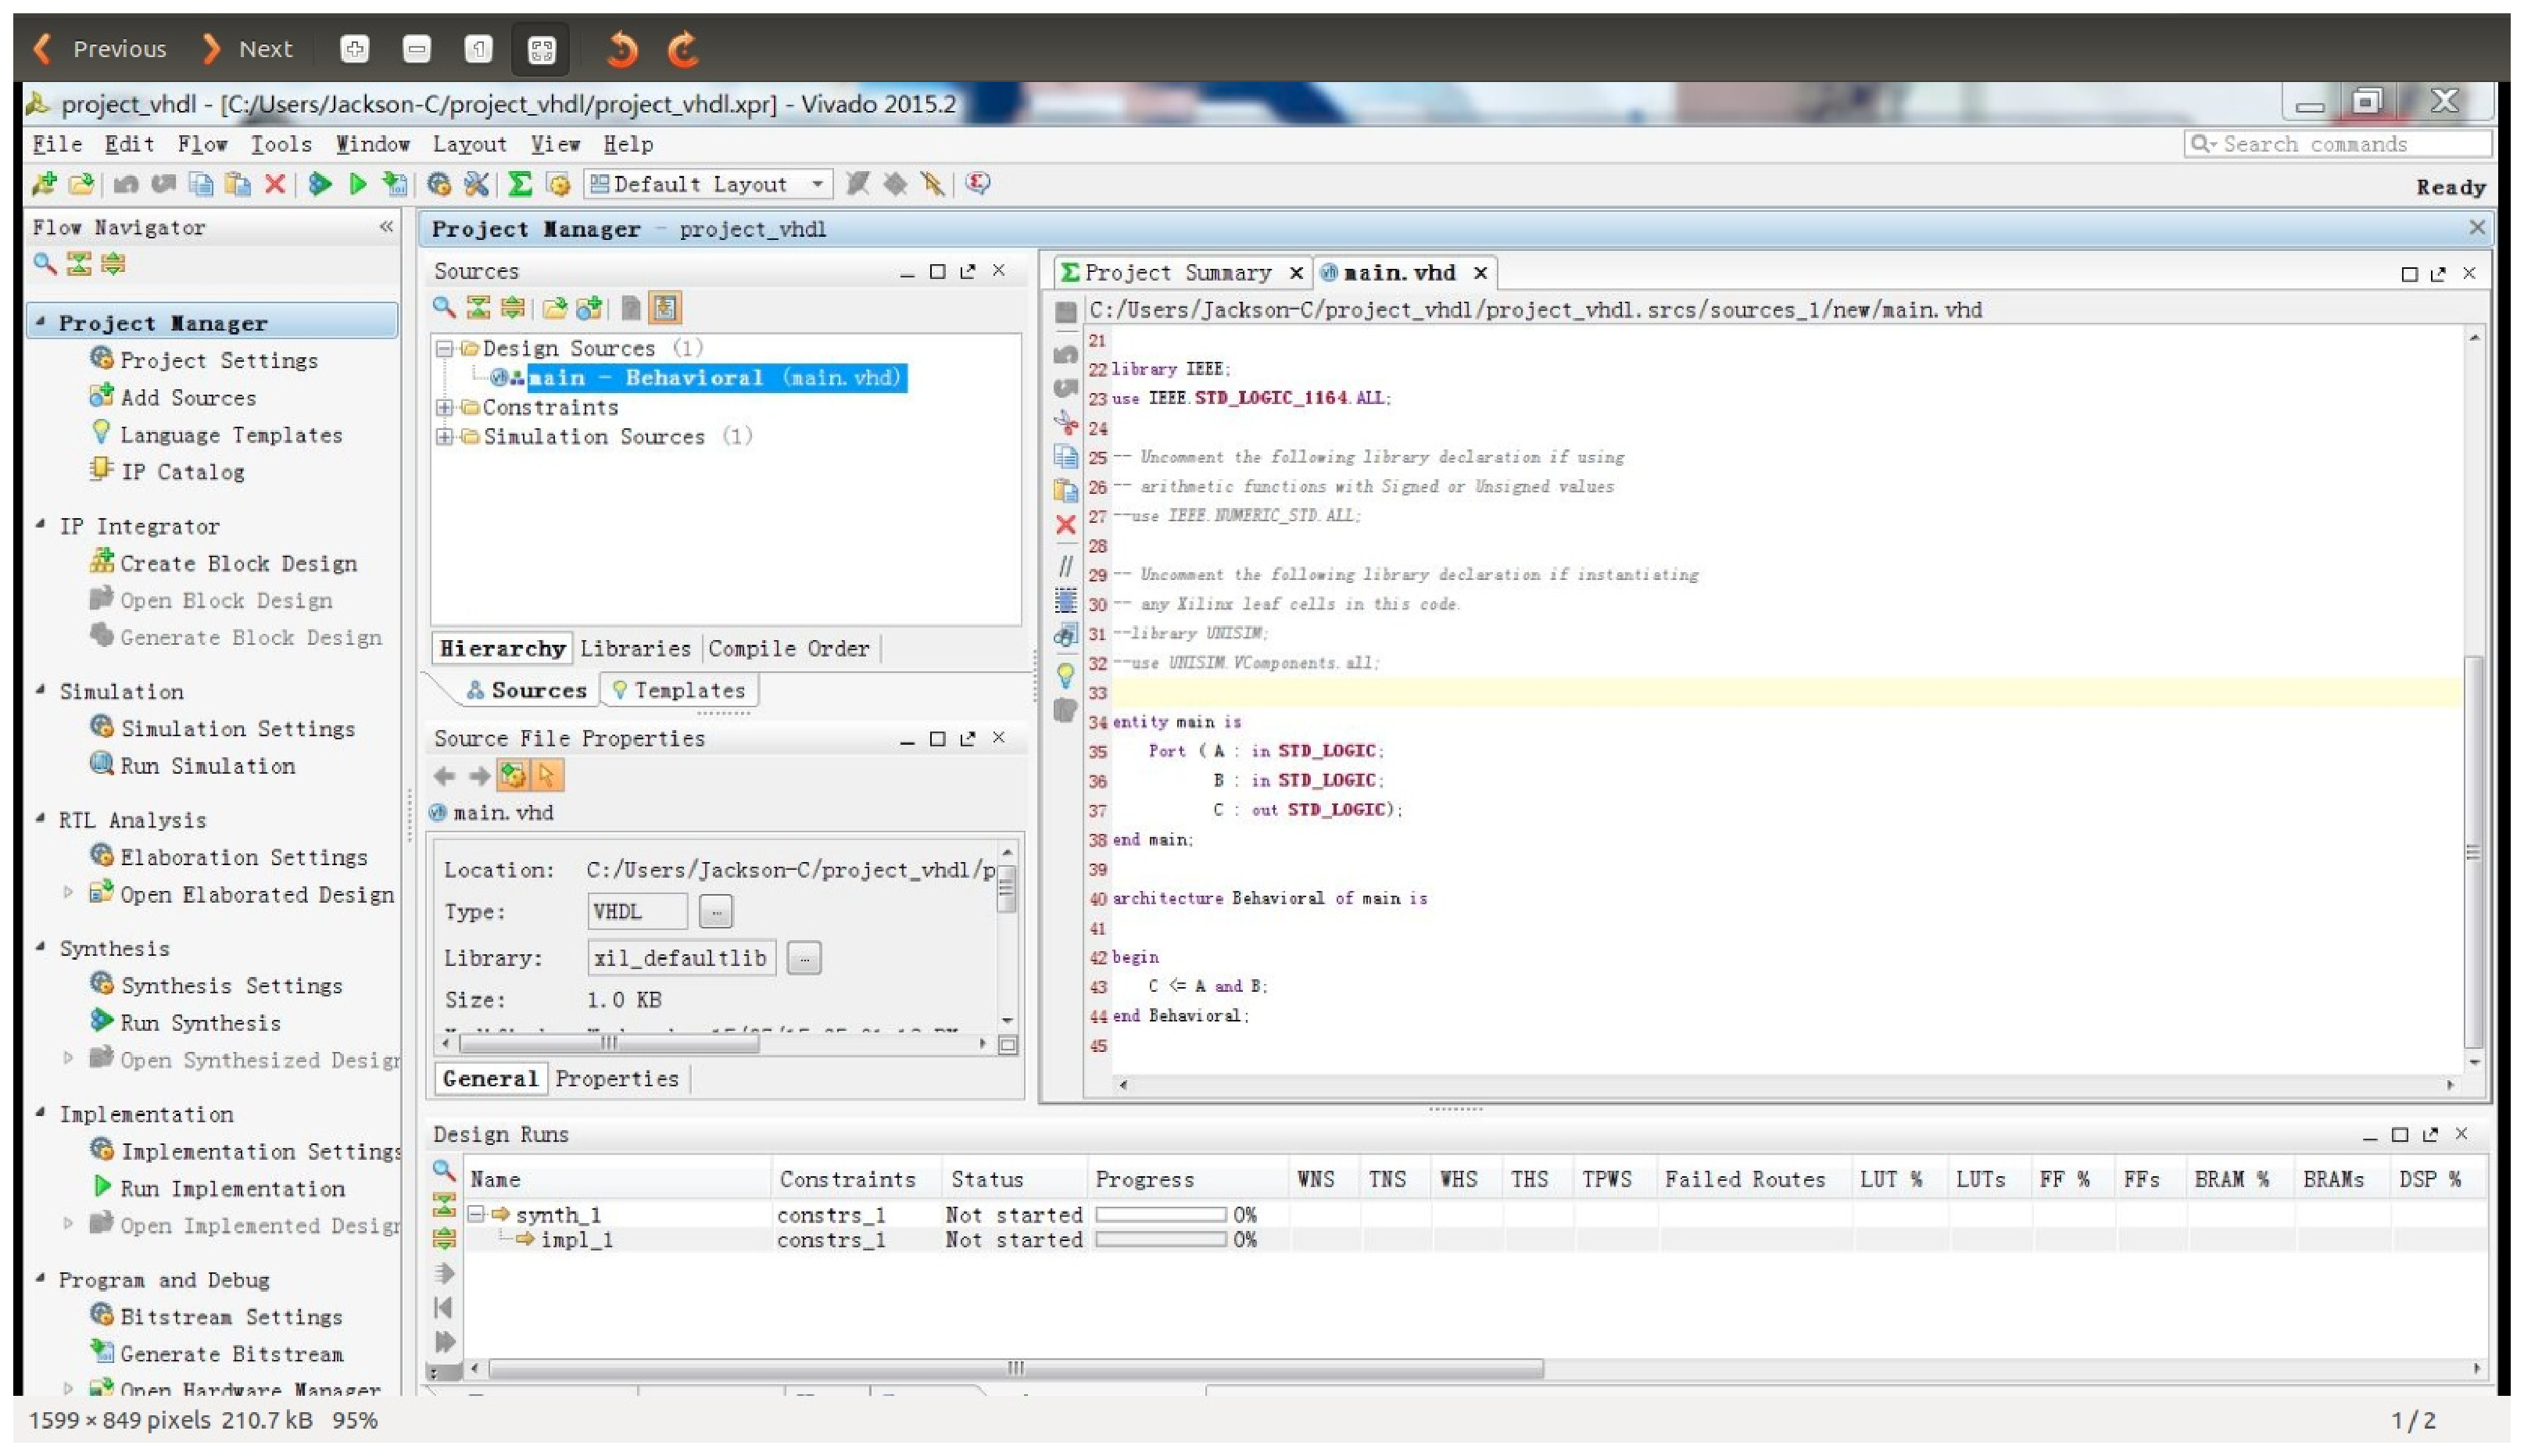
\includegraphics[scale=0.25]{eps/vivado1.eps}
\caption{The vivado1}
\label{vivado1}
\end{figure}

As can be seen in Figure~\ref{vivado1}, the code we use to illustrate
the vivado workflow is simple. two input signals A and B, one output
signal C. The transformation logic between them is: C $<=$ A and B.

The code:

\begin{chunk}{ANDvhdl}

library IEEE;
use IEEE.STD_LOGIC_1164.ALL;

entity main is
	For: (A:in STD_LOGIC;
		B:in STD_LOGIC;
		C:out STD_LOGIC);
end main;

architecture Behavioral of main is

begin
	C<=A and B;
end Behavioral;

\end{chunk}


\begin{figure}[ht!]
\centering
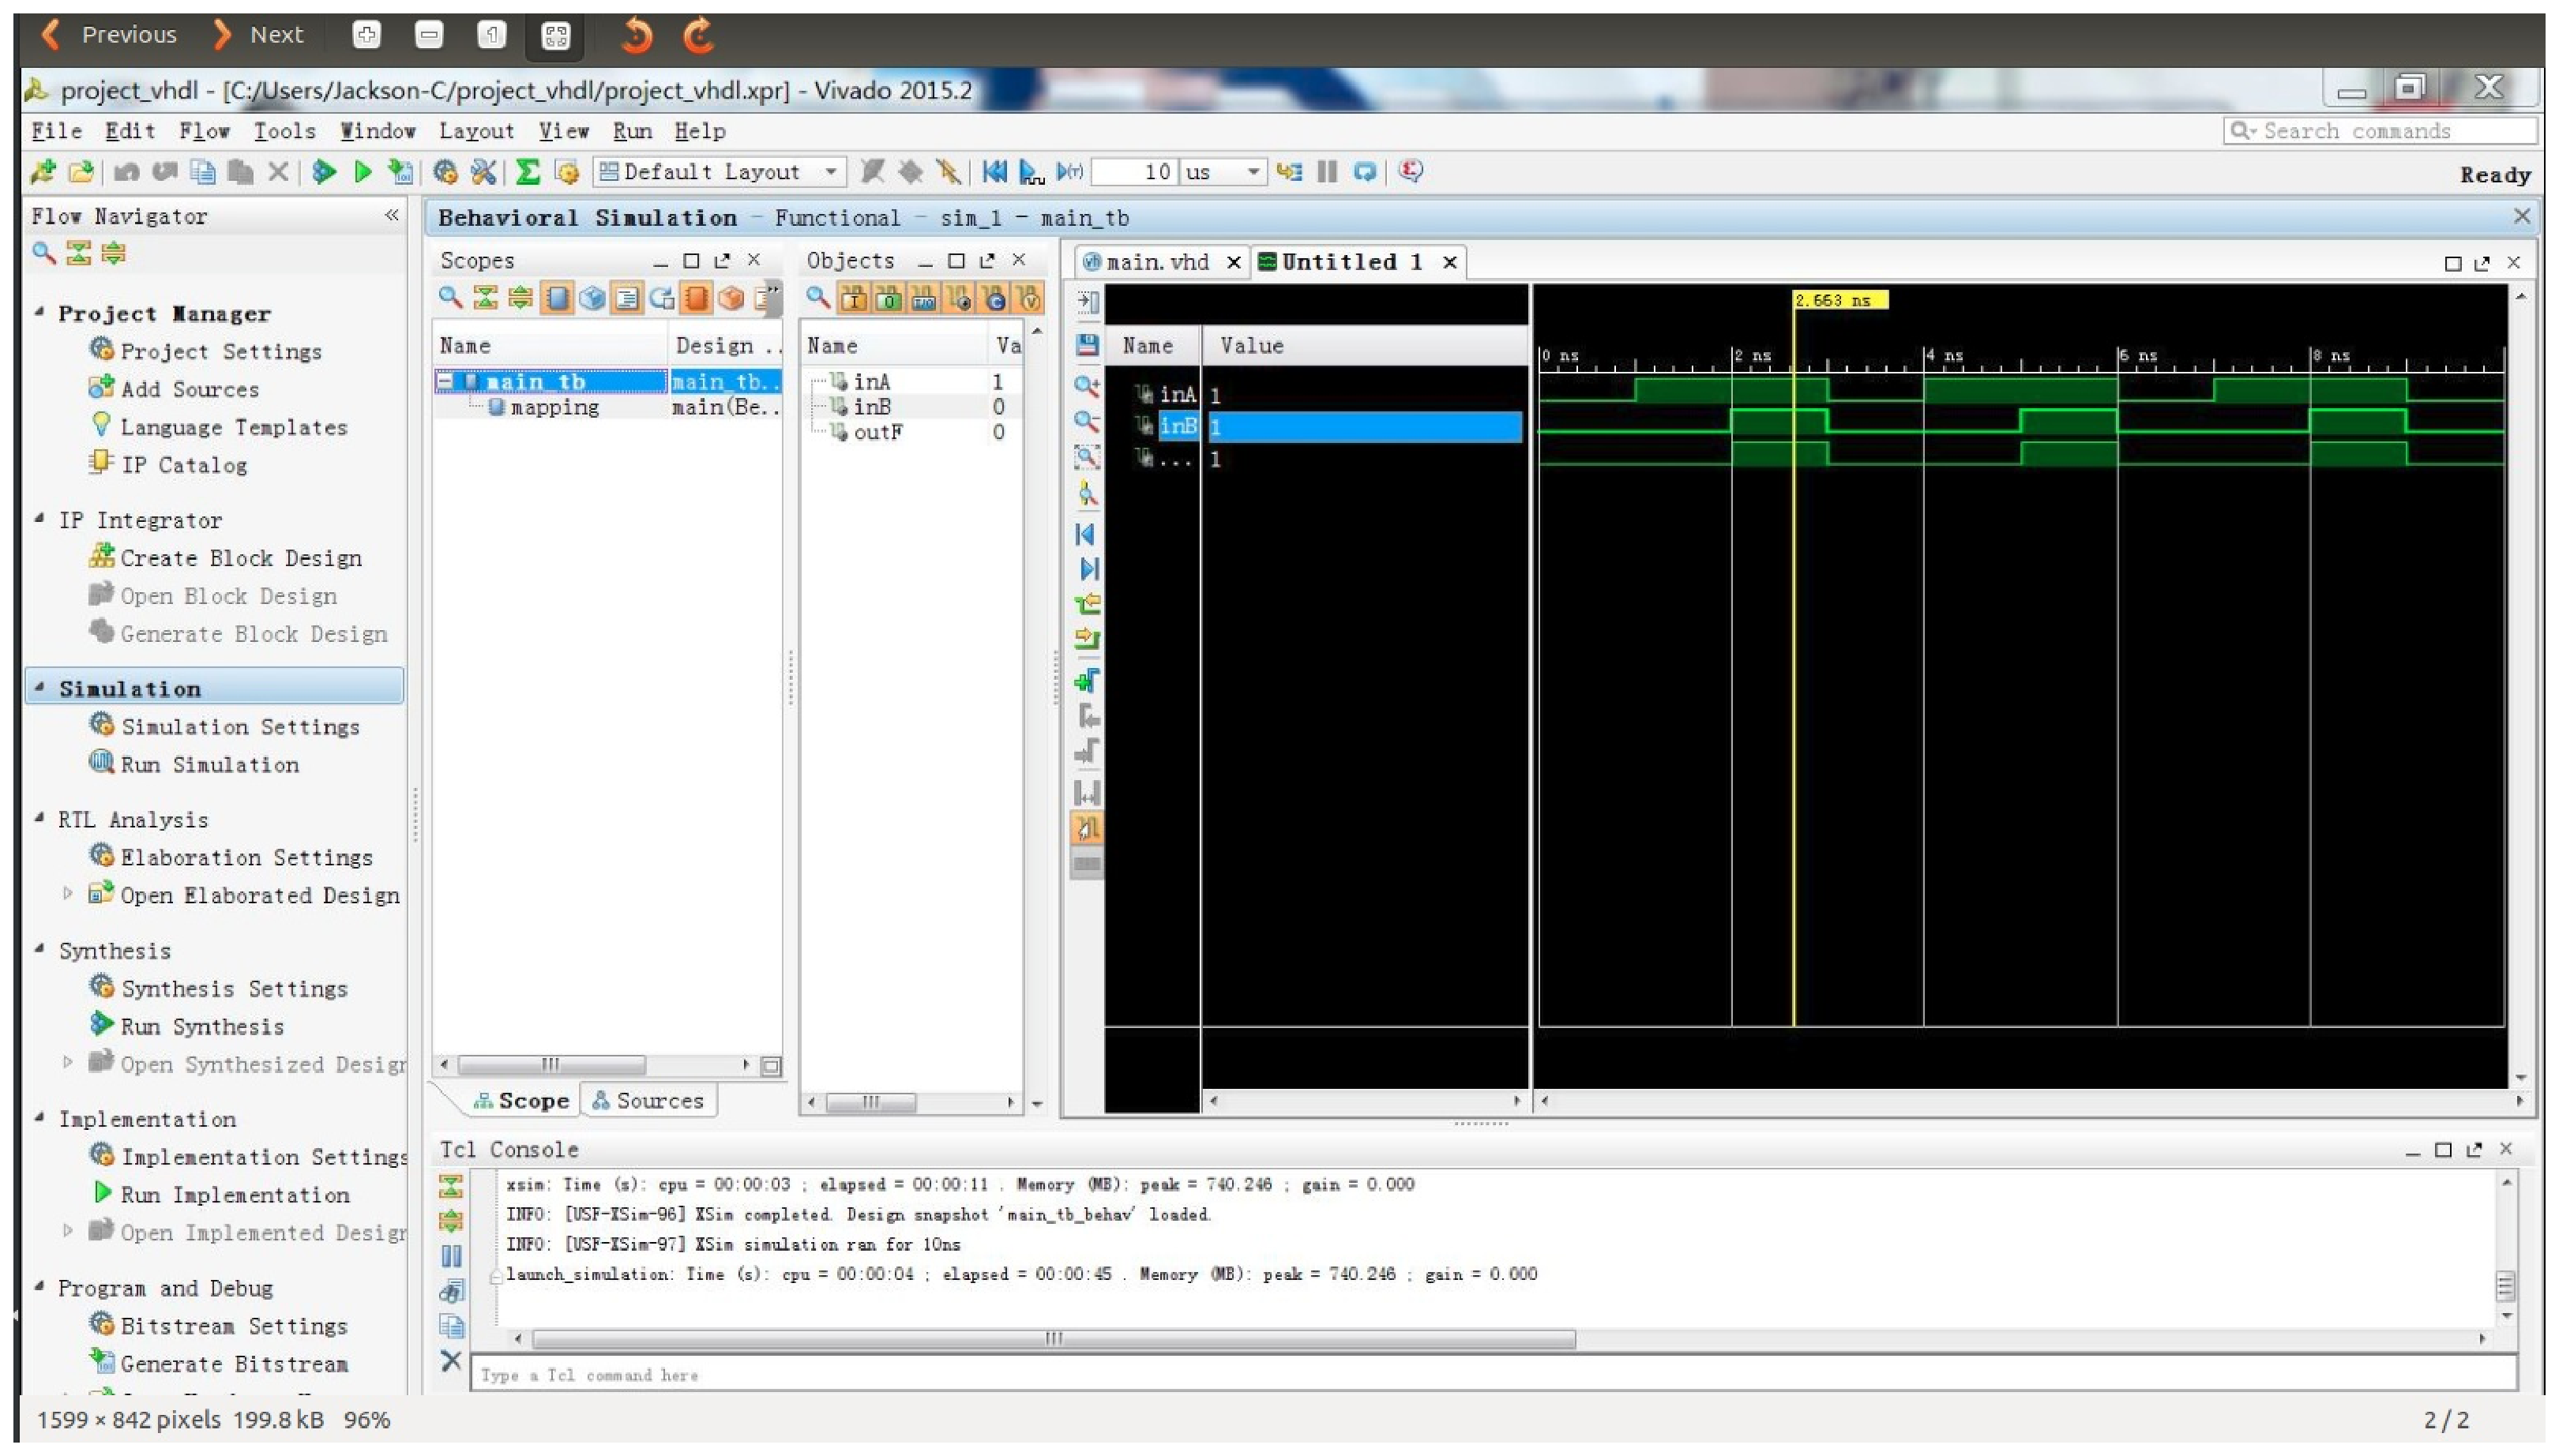
\includegraphics[scale=0.25]{eps/vivado2.eps}
\caption{The vivado2}
\label{vivado2}
\end{figure}

As can be seen in Figure~\ref{vivado2}, we can find the waveform after
simulating the vhdl code we presented above and it's easy to see the
transformation logic behind the scenes.

Some Useful video links to use Vivado:


Vivado Design Flows Overview (v2013.1): From \cite{59}

This video briefly describes the Vivado Design workflow. There are two
Use Models:
\begin{enumerate}
\item Tcl scripted or GUI based use models
\begin{itemize}
\item Run entire flow manually using Vivado Tcl Shell commands or scripts
\item Run entire flow with the press of a button using the Vivado IDE
\end{itemize}
\item Batch compilation style flow or project based flow
\begin{itemize}
\item Manually manage all sources, design commands and configuration, and
reporting using Tcl commands and scripts (Non-Project Mode)
\item Create a Project infrastructure on disk to manage entire design
process and track status (Project Mode)
\end{itemize}
\end{enumerate}
And some other things to be mentioned:
\begin{enumerate}
\item IP-Centric System-level Design Integration
\begin{itemize}
\item Create IP subsystems with IP Integrator
\item Configure, validate and instantiate IP using the IP Catalog
\end{itemize}
\item System Design Entry through Hardware Validation Flows
\begin{itemize}
\item Advanced design, analysis and process management capabilities
\end{itemize}
\item Flexible Use Models
\begin{itemize}
\item Tcl accessible common data model throughout the flow
\item Project and compilation style flows
\item Support for third party software tools
\end{itemize}
\item Programming and Debugging Design in Hardware: From \cite{60}:\\
This video briefly explains and shows the steps to program and debug
in Hardware using Vivado:
\begin{enumerate}
\item Connecting to the hardware and programming the FPGA
\item Setting up the ILA debug core trigger and probe simple compare conditions
\item Arming the ILA debug core and capture data in the waveform window
\end{enumerate}
\item Logic Simulation: From \cite{61}:

This video shows how to simulate a design in Vivado IDE:
\begin{enumerate}
\item Simulation Settings
\item Launching Vivado Simulator
\item Waveform Viewer
\end{enumerate}
\end{enumerate}

And it lists some of the advantages that Vivado provides:
\begin{enumerate}
\item Easy to manage simulation sources and settings
\begin{itemize}
\item automatically compile and simulate sources
\end{itemize}
\item Fully integrated simulator
\begin{itemize}
\item powerful simulator engine (3x faster than ISE Simulator)
\item Common waveform viewer
\end{itemize}
\end{enumerate}

And that could be part of the reasons why we choose Vivado rather than ISE.


\chapter{MAC}

Here, we are using the tri-mode ethernet MAC v0.1.

\begin{enumerate}
\item Introduction

The core of the Tri-mode ethernet MAC is designed from the ground up to be a compact, fast, no-frills core to faciliate streaming data from a widget to a connected computer. For example, the core only supports full-duplex operation in that it does not even look at the CRS (carrier-sense) and COL (collision detection) signals from the PHY (physical layer). And it will generate the ethernet and udp headers so we can simply give it data and it will take care of sending it for us.

\item Features

• Interfaces with the PHY using GMII running 10/100/1000 Mb/s. Support for RGMII is planned.
• Full-duplex support only.
• Raw ethernet frame generation, allowing a pure data input stream.
• Optional UDP/IP packet generation with automatic packetization and framentation of an input data
stream.
• Input and output fifos decoupled from the core logic, so the clock rate of application logic is not tied
to the speed of the ethernet link (barring bandwidth issues).
• Full core uses 288 Spartan 6 logic slices and 2 block RAMs. For comparison, the smallest Spartan 6
has 600 slices and 12 block RAMs. The largest Spartan 6 has 23,038 slices and 268 block RAMs.

\item Interfaces

\begin{itemize}

\item Parameters

\begin{figure}[ht!]
\centering
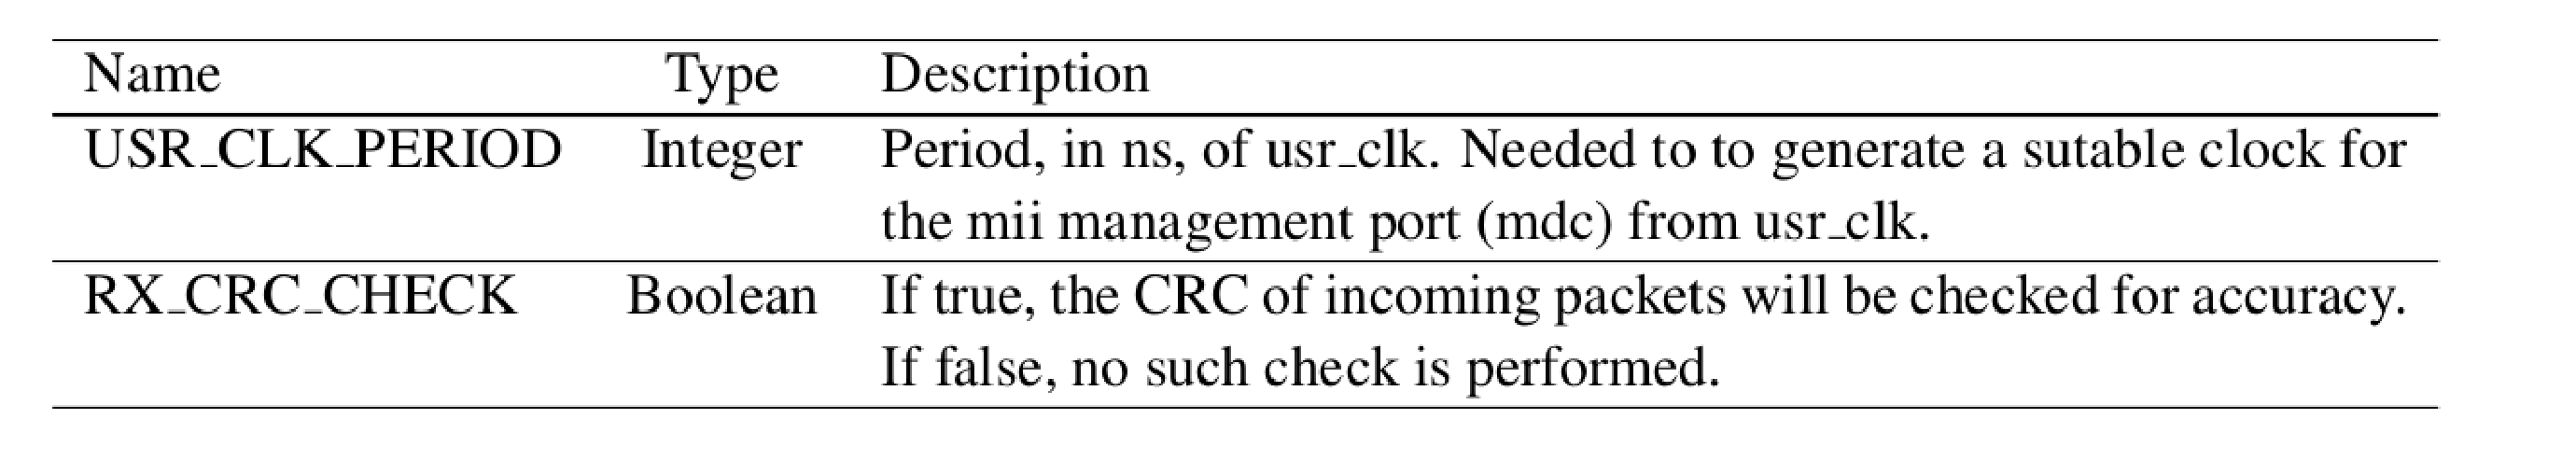
\includegraphics[scale=0.25]{eps/mac1.eps}
\caption{The mac1}
\label{mac1}
\end{figure}

\item Clocks, etc.

\begin{figure}[ht!]
\centering
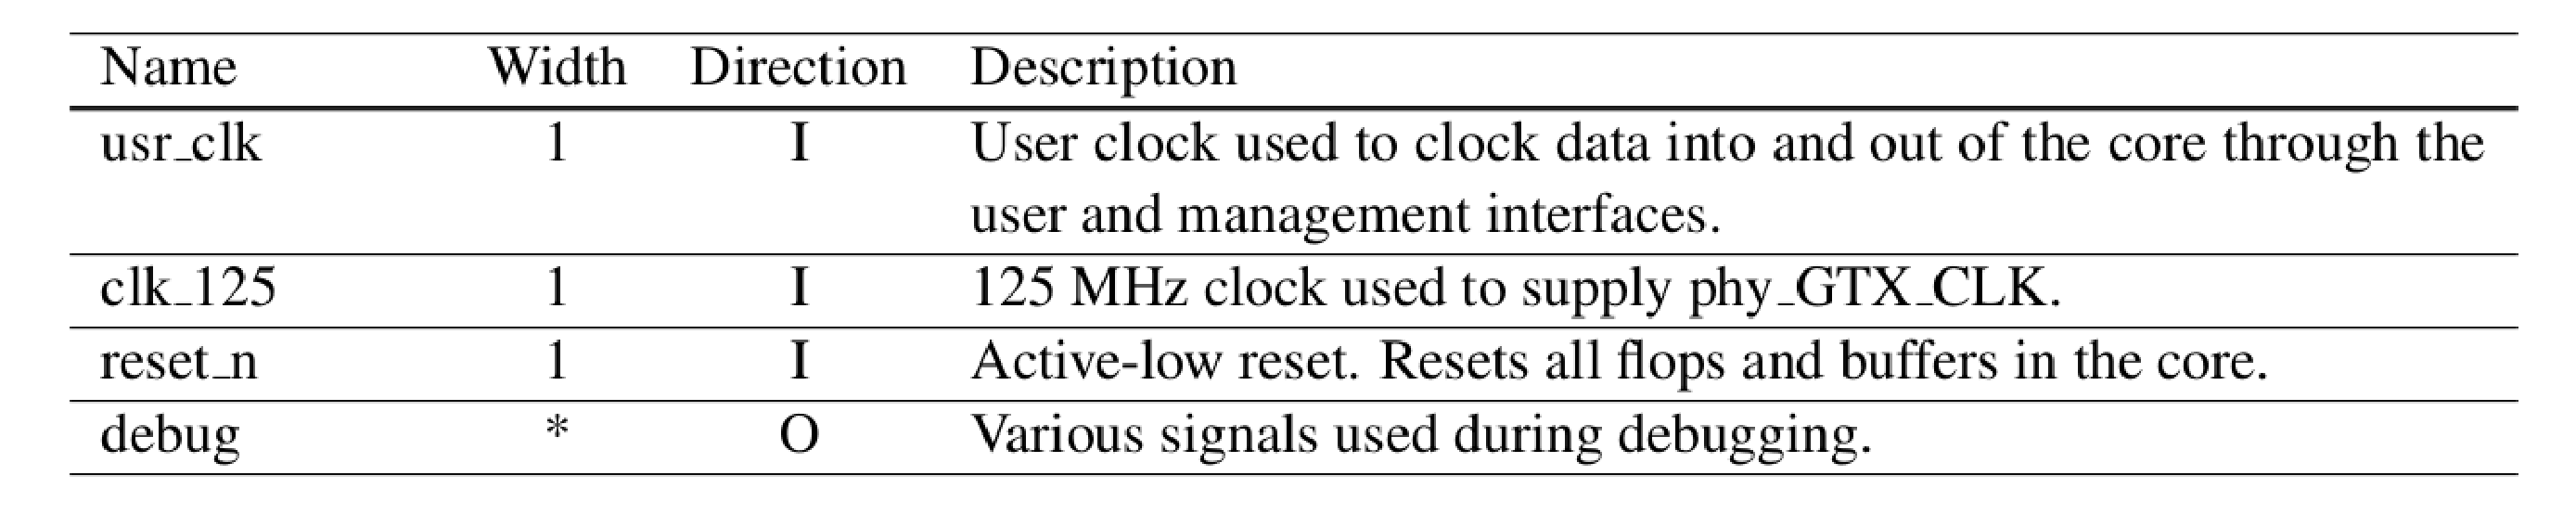
\includegraphics[scale=0.25]{eps/mac2.eps}
\caption{mac2}
\label{mac2}
\end{figure}

\end{itemize}

\item Configuration

Instead of implementing internal registers to indicate the source and destination MAC address, these values are simply ports into the core. 

\begin{figure}[ht!]
\centering
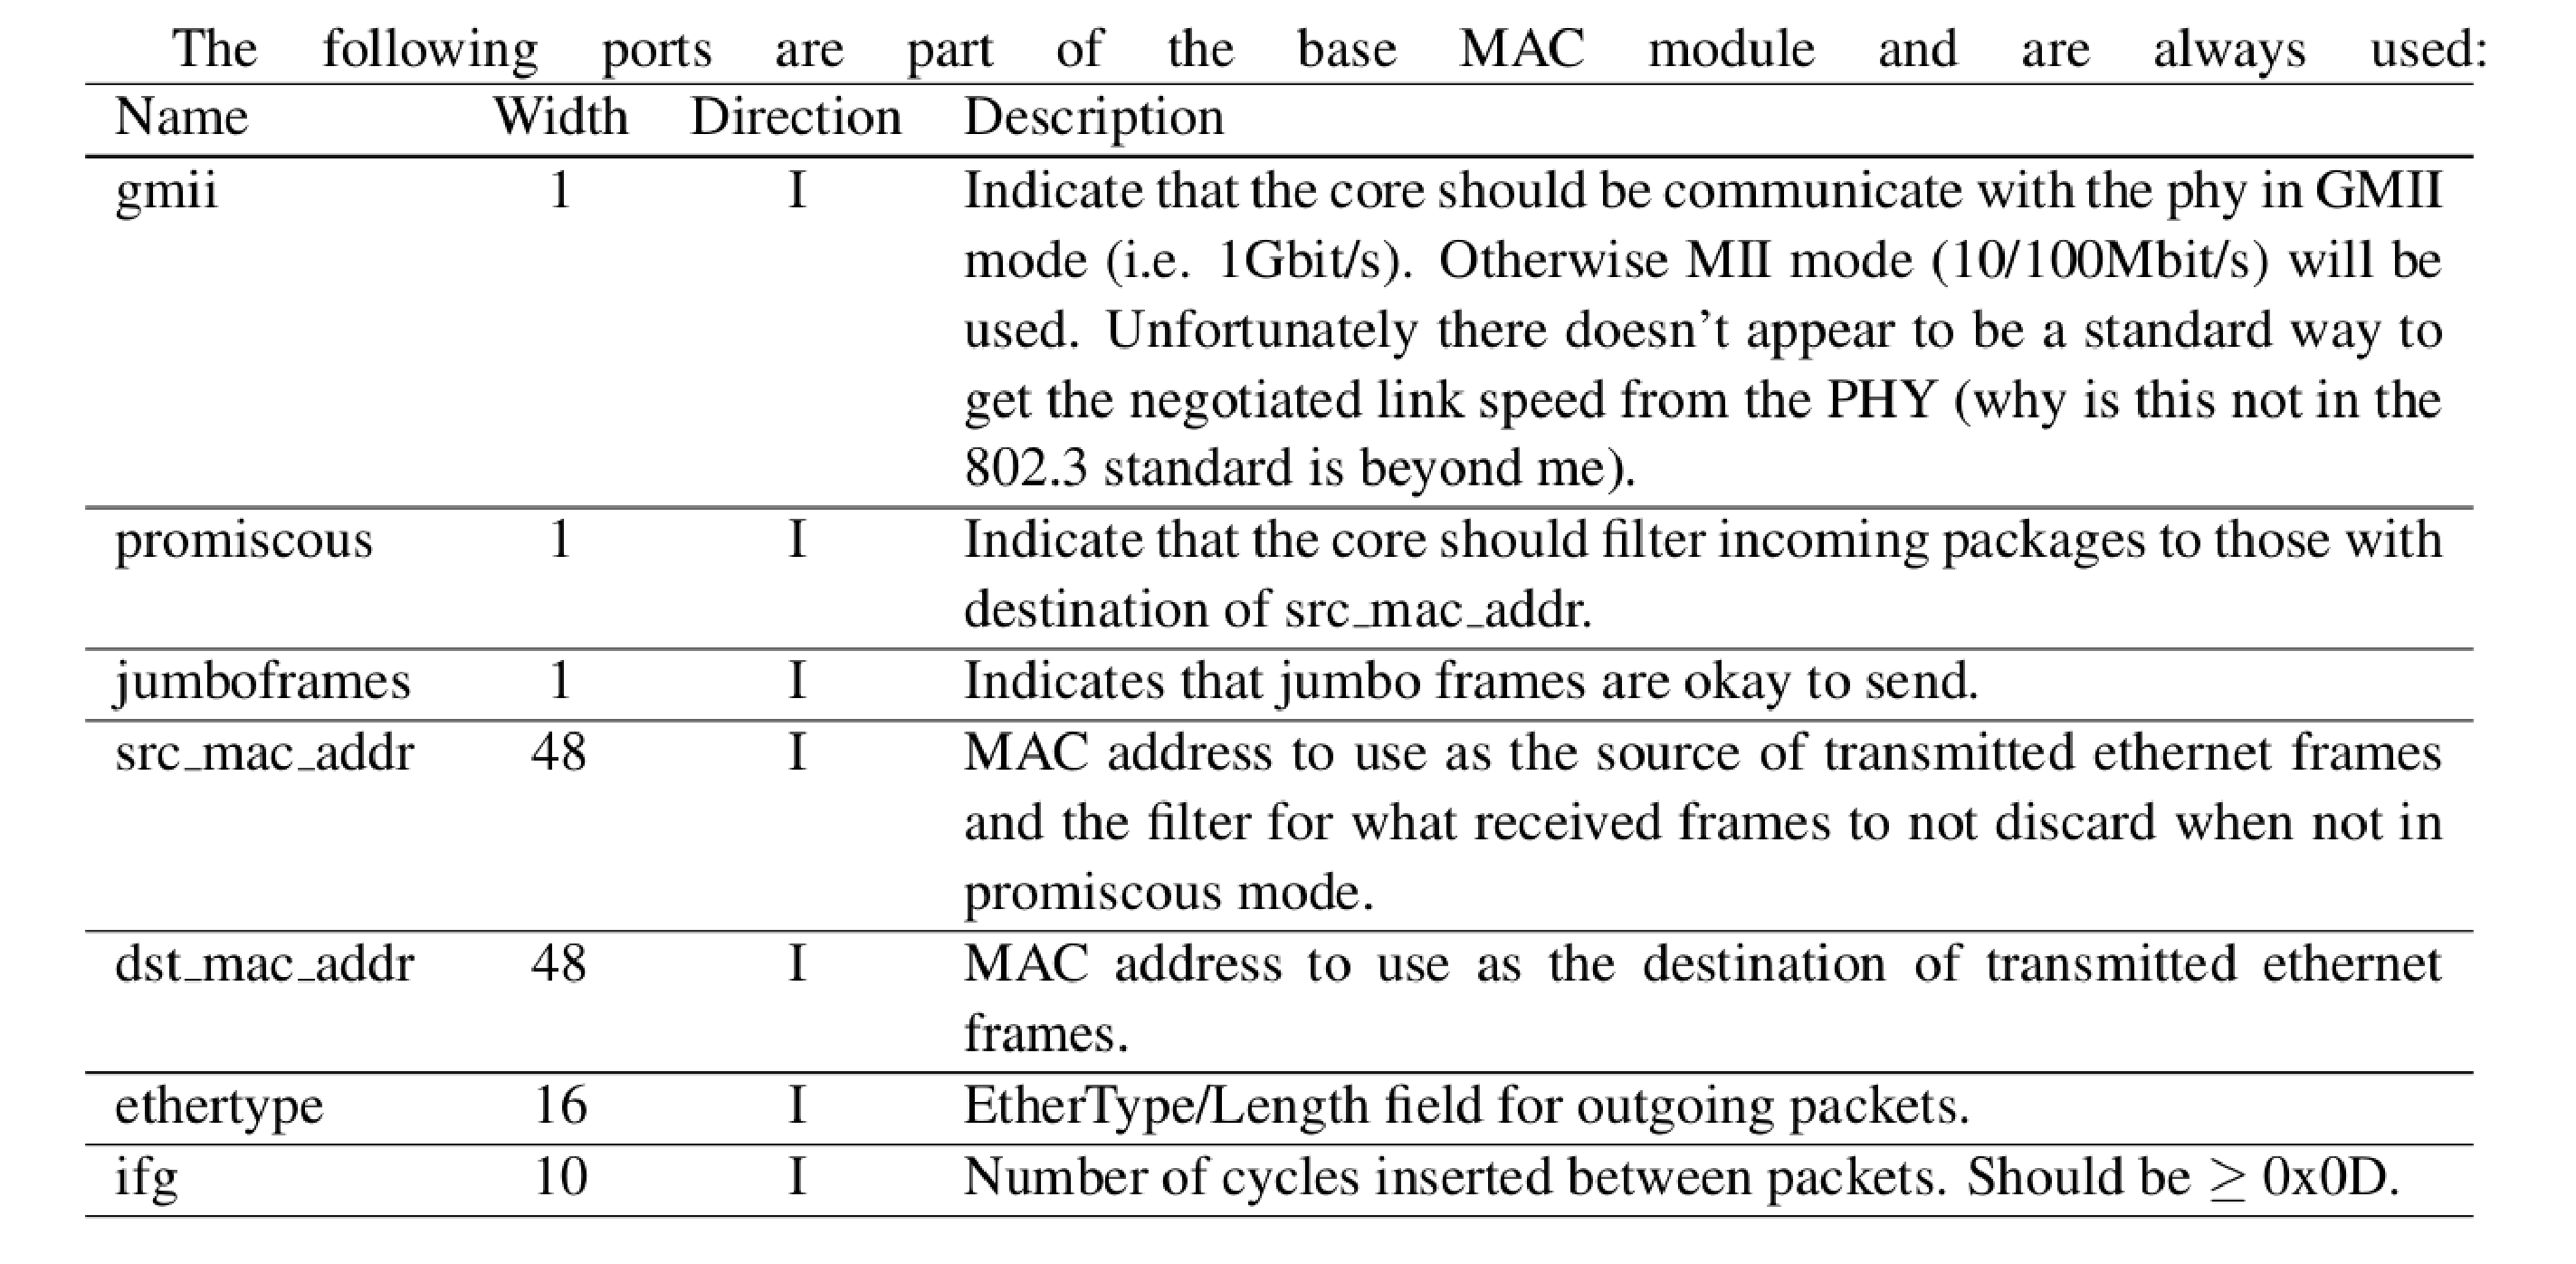
\includegraphics[scale=0.25]{eps/mac3.eps}
\caption{mac3}
\label{mac3}
\end{figure}

\begin{figure}[ht!]
\centering
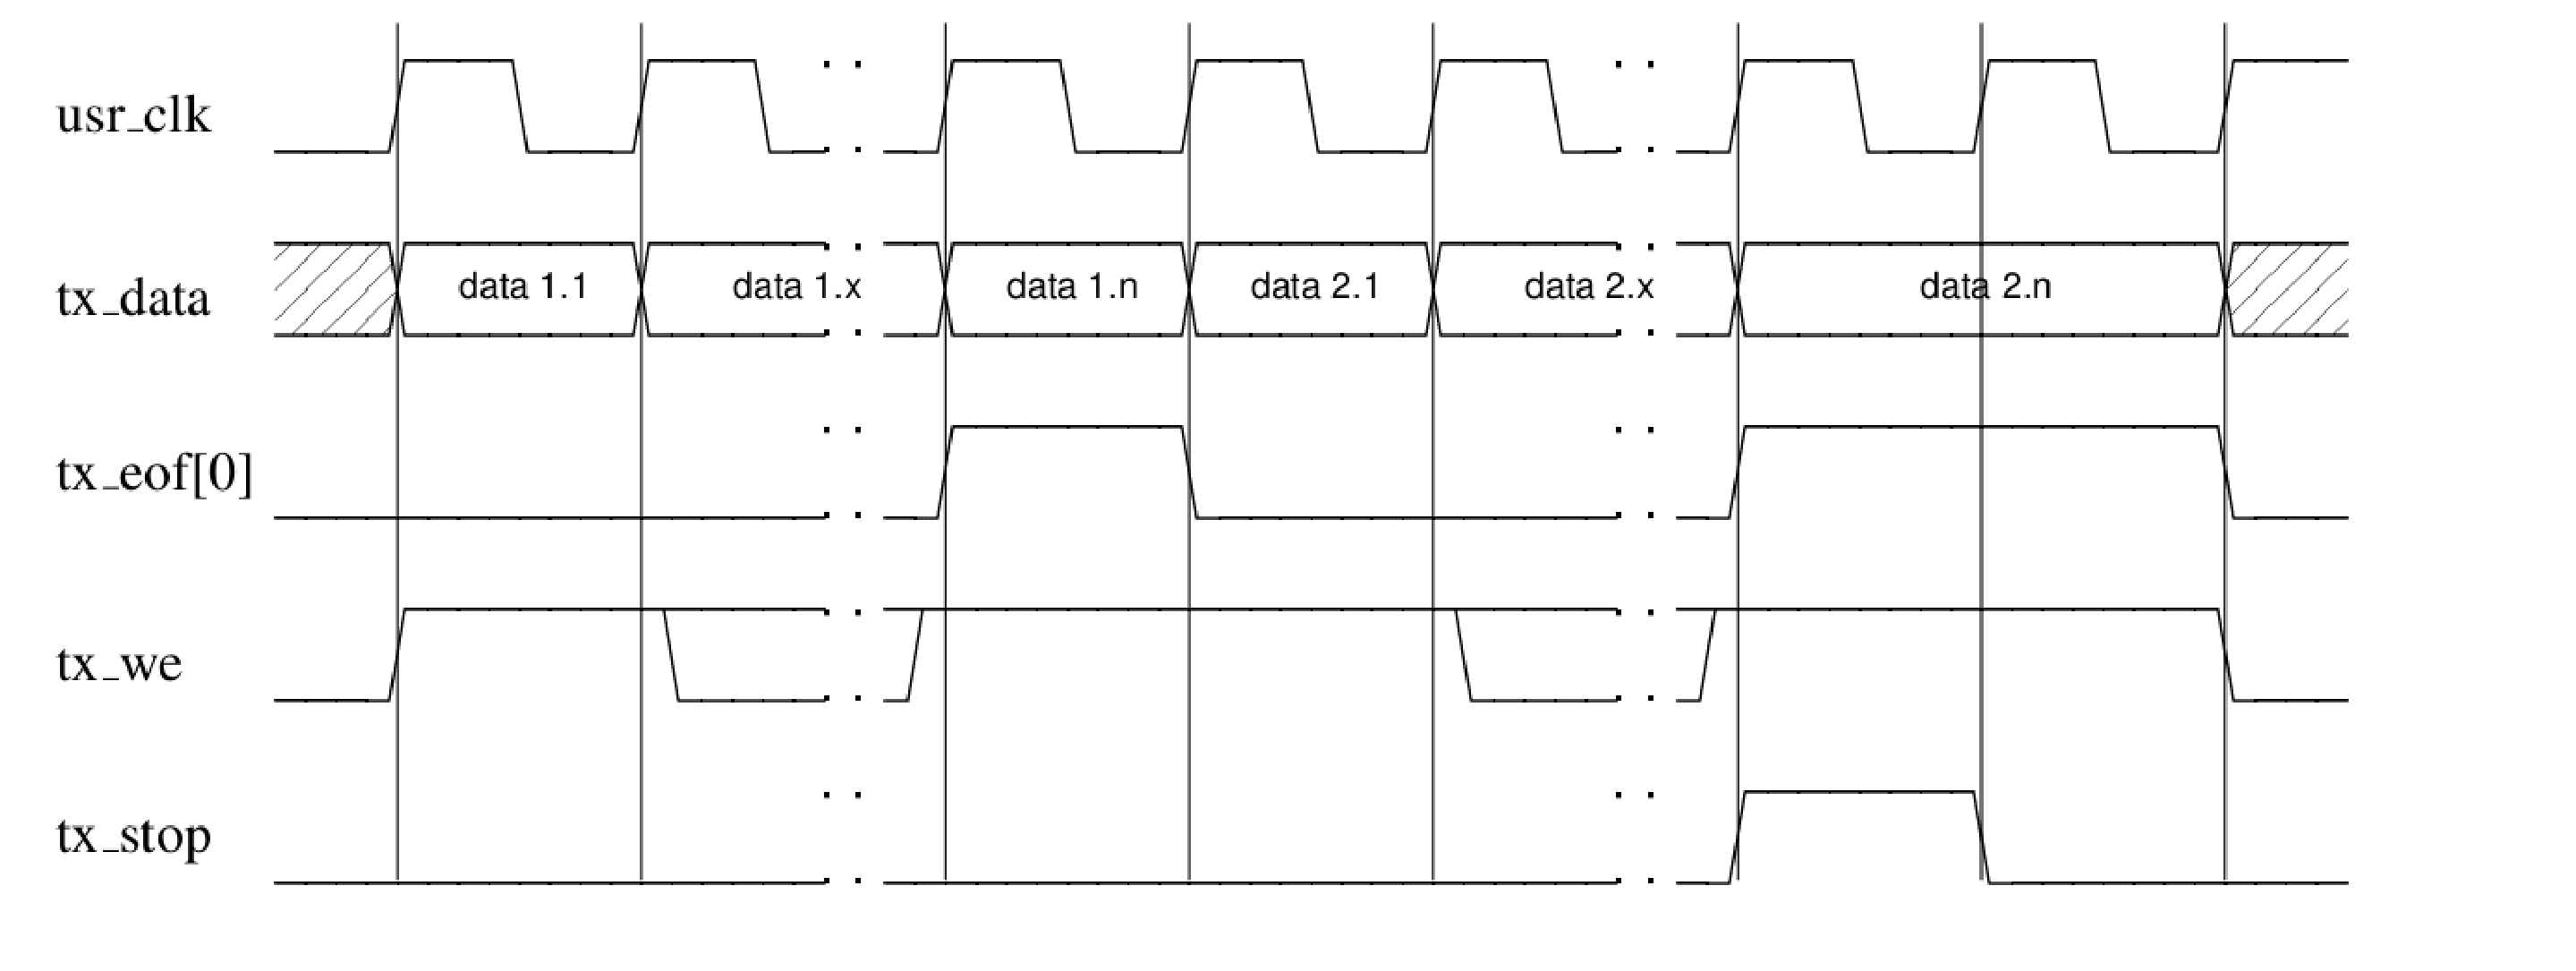
\includegraphics[scale=0.25]{eps/mac4.eps}
\caption{mac4}
\label{mac4}
\end{figure}

In Figure~\ref{mac4}, we can see the timing diagram of two back to back 32-bit aligned packet transmissions, with the final word of the second packet being interrupted by a full input fifo.

\item Transmission

The interface used to send packets/frames is a standard FIFO write interface with addition of an end-of-frame port (tx eo f ) that is used to split incoming data into frames.

\begin{figure}[ht!]
\centering
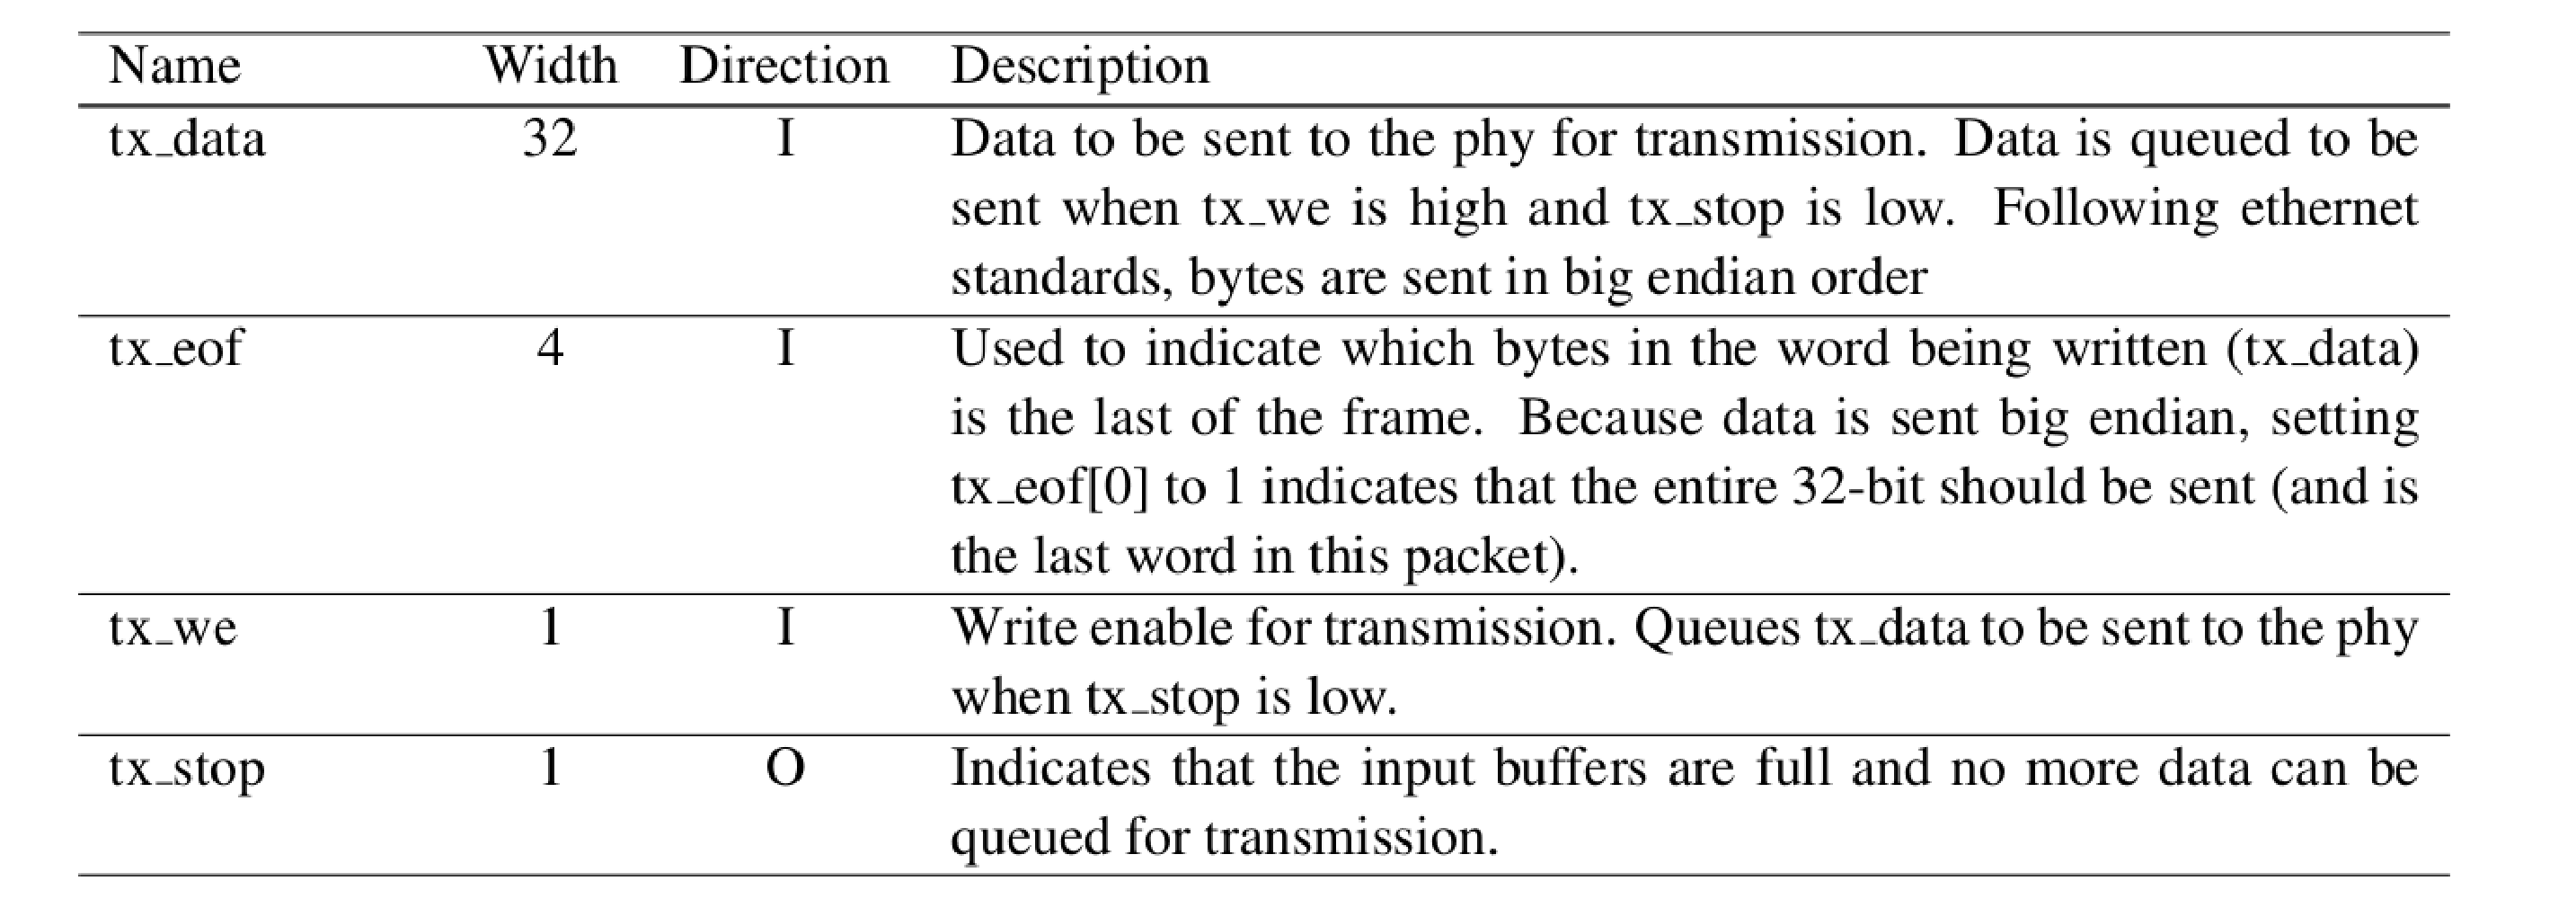
\includegraphics[scale=0.25]{eps/mac5.eps}
\caption{mac5}
\label{mac5}
\end{figure}


If the input fifo runs out of data while the MAC is sending a packet, an error condition will be raised and the packet will not be sent. Operating at 1Gbps, the PHY will transmit approximately 100MB/s from the input fifo. Therefore, if data word is supplied every clock, the user clock must be at least 25 MHz, an easy target for most FPGAs. Alternatively, if the user clock is faster, data need not be supplied on each clock. For example, a 100 MHz user clock means that once data is first written to the input fifo, the rest of the data can come at a rate as slow as one word every 4 clocks.


\item Reception

The interface used to receive packets is a standard FIFO read interface, with the addition of an end-of-frame port (rx eo f ).

\begin{figure}[ht!]
\centering
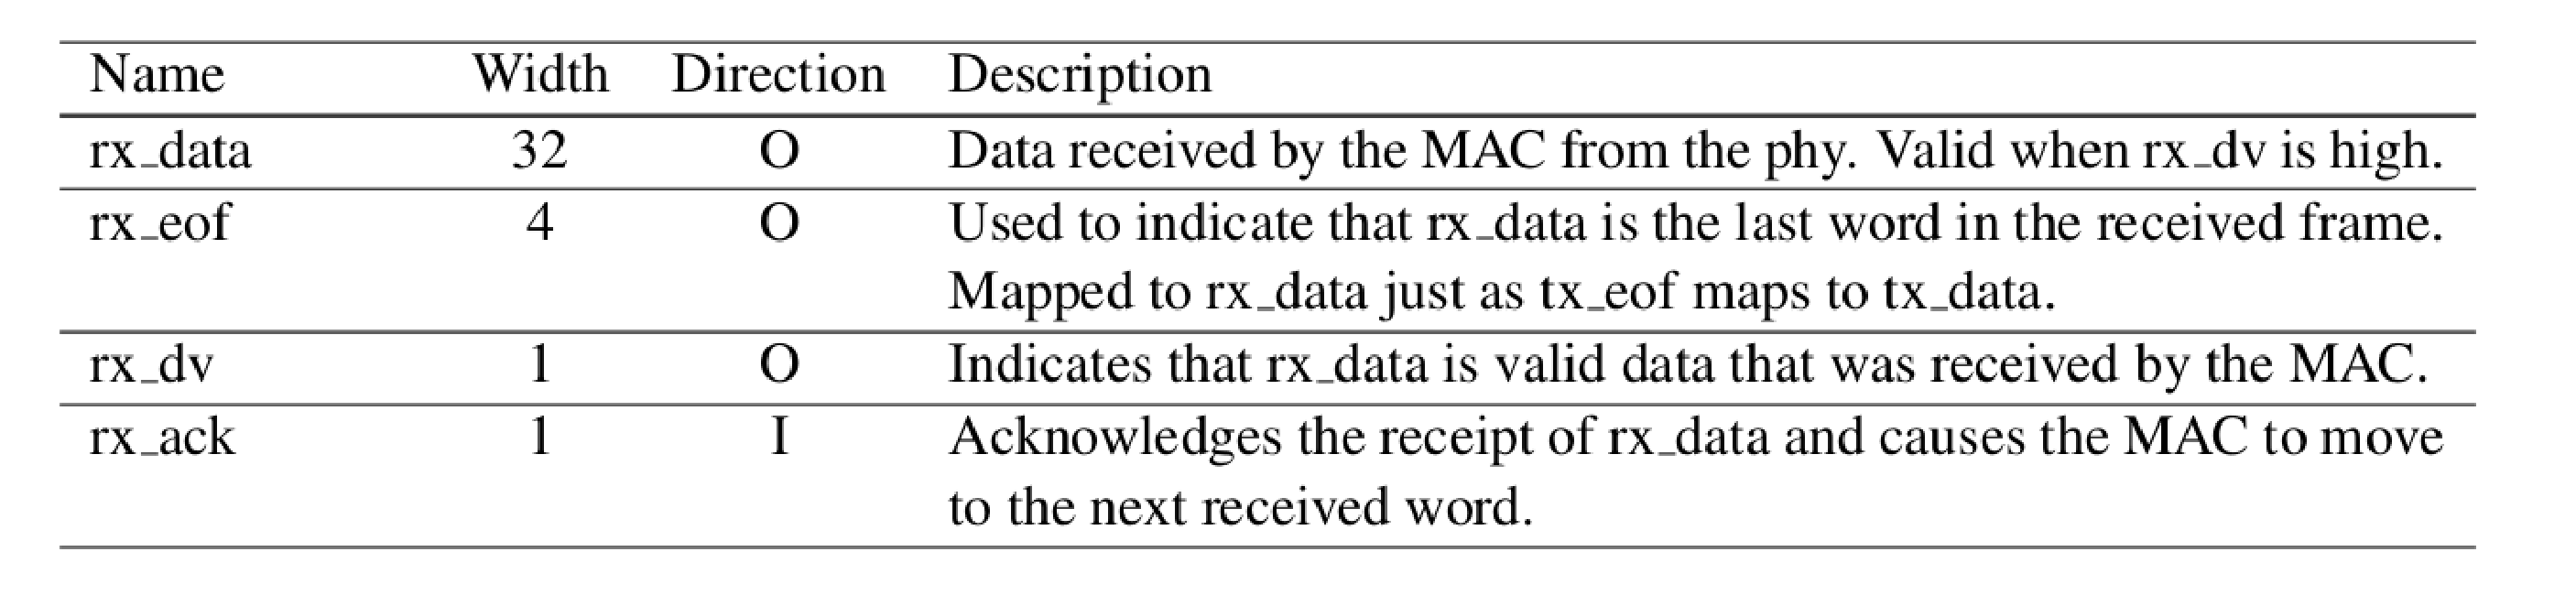
\includegraphics[scale=0.25]{eps/mac6.eps}
\caption{mac6}
\label{mac6}
\end{figure}

\item Management

The following ports are used to read and write the MII management registers on the PHY. If they are left unconnected, the MII management module will be optimized away by the synthesis tools.

\begin{figure}[ht!]
\centering
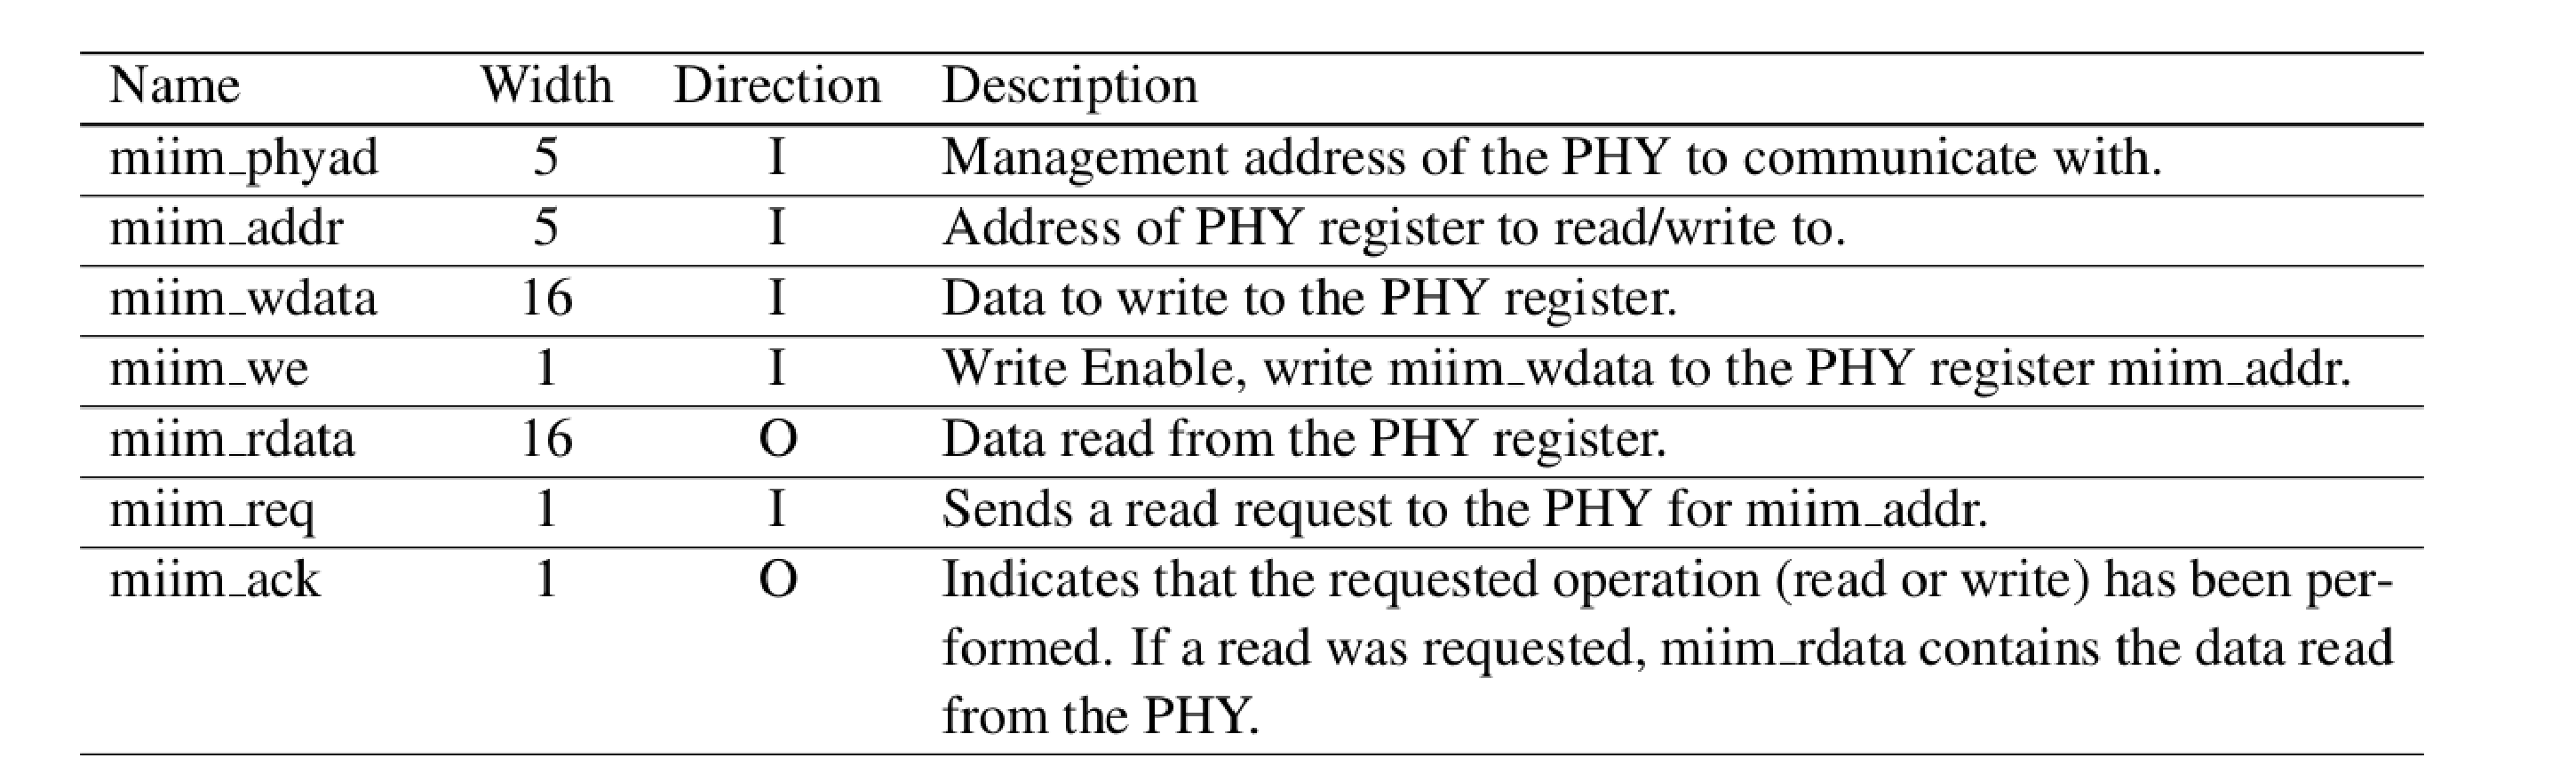
\includegraphics[scale=0.25]{eps/mac7.eps}
\caption{mac7}
\label{mac7}
\end{figure}

\item UDP/IP

When the UDP/IP Wrapper is used, the ethertype port is removed and the following configuration ports are added.

\begin{figure}[ht!]
\centering
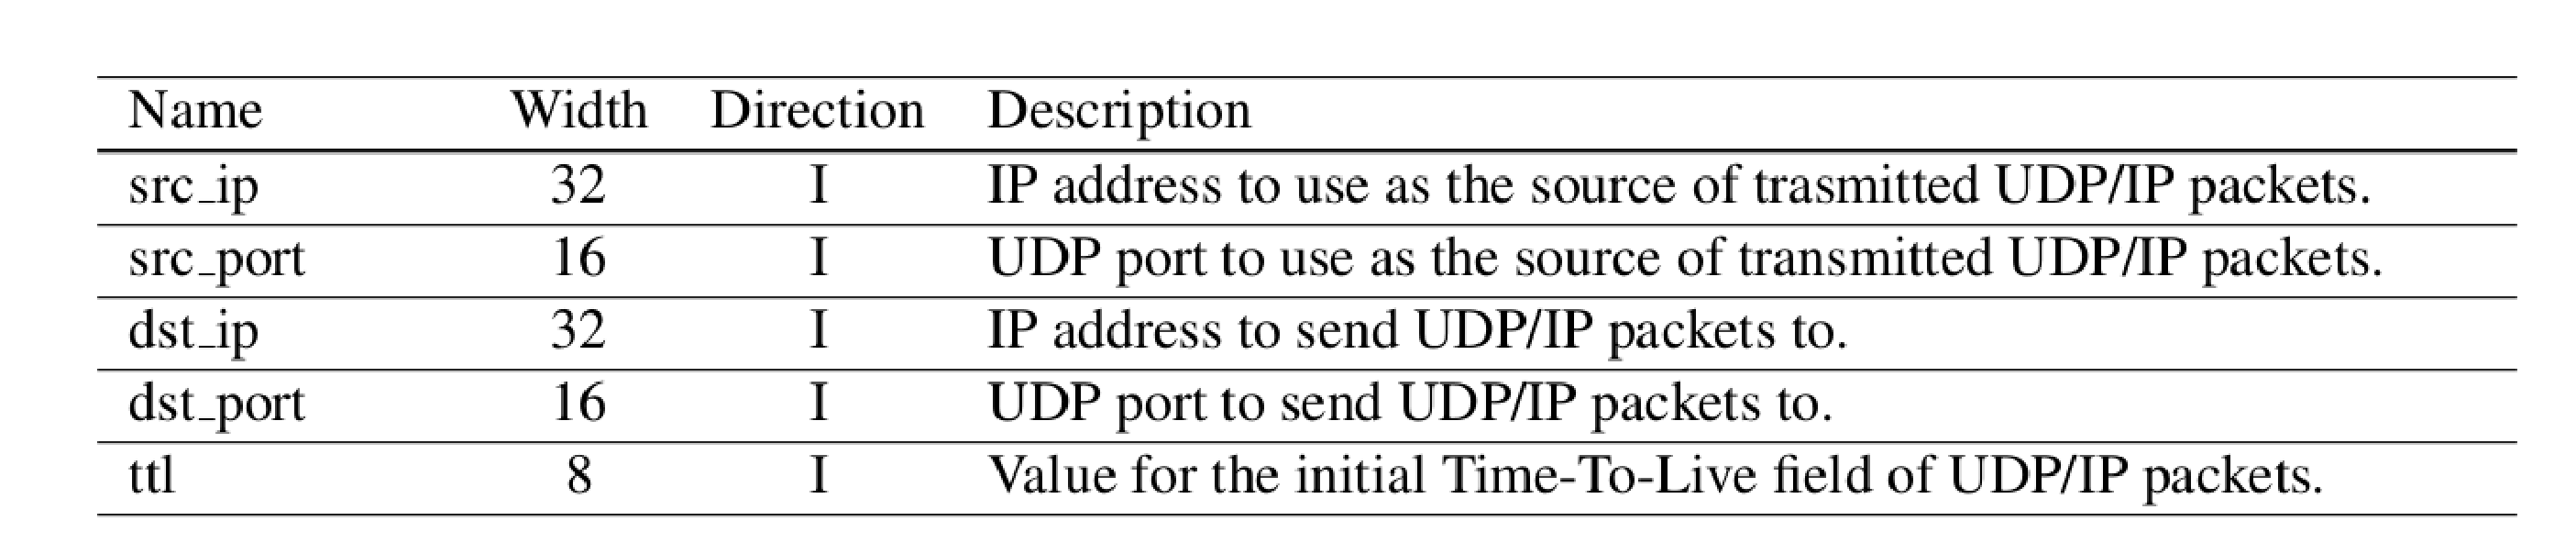
\includegraphics[scale=0.25]{eps/mac8.eps}
\caption{mac8}
\label{mac8}
\end{figure}


\item PHY

The PHY ports are the standard GMII ports that should be tied directly to pins connected to an ethernet PHY.

\begin{figure}[ht!]
\centering
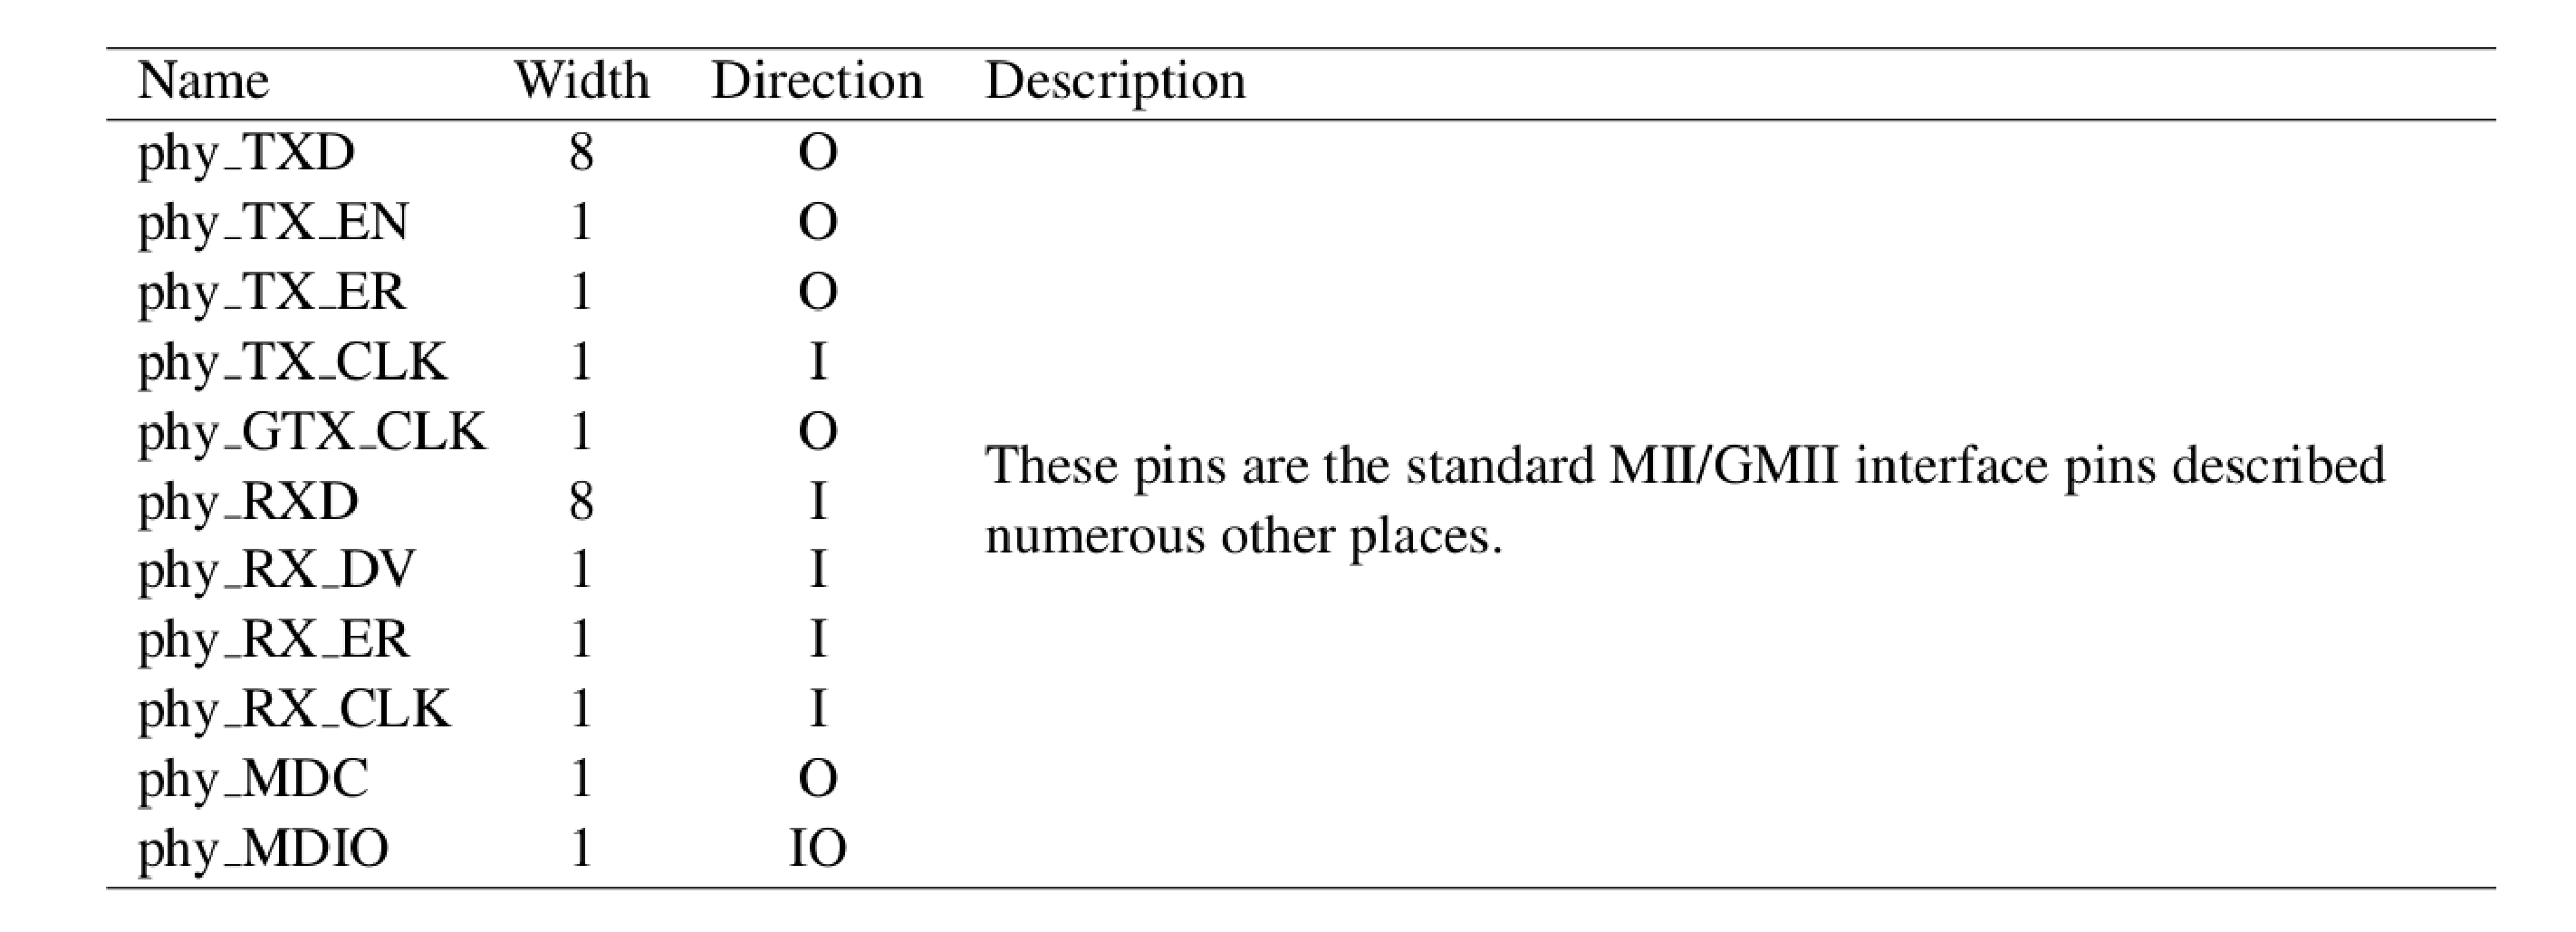
\includegraphics[scale=0.25]{eps/mac9.eps}
\caption{mac9}
\label{mac9}
\end{figure}

\item Reconciliation

The reconcilation modules provides a common interface to the rest of the core regardless of the speed of the ethernet link. This is done by providing internal clocks to both the tx (int tx clk) and rx (int rx clk) modules which can be used to send data to the reconciliation layer eight bits a clock.

If gmii is high we are operating at gigabit speeds and the phy sends and receives a full eight bits of data each 8ns. For transmission, clk 125 is used as both int tx clk and sent as phy GTXCLK, synchronizing all tranmission to that one 125 MHz clock. Likewise, all reception is synchronized to the 125 MHz phy RXCLK, which is sent as int rx clk.

If gmii is low we are operating at 10 or 100 Mbits per second and only four bits of the databus to the phy is used. For transmission, the phy expects four bits every cycle of the phy supplied phy TXCLK; to maintain an eight bit interface with the rest of the mac, phy TXCLK is divided in half and sent as int tx clk. Likewise, the phy sends four bits every phy RXCLK, so this is divided in half and sent as int rx clk.


\item Architecture

The MAC core is split up into three main components: tranmission, reception, and reconciliation. The transmission blocks, txfifo, tx engine, and crc gen, are responsible for taking user data and sending it to the reconcilia- tion module, which sends it to the ethernet phy. Likewise the recption blocks, rx usr if, rx pkt fifo, rxfifo, rx engine, and crc chk, are responsible for taking data from the reconciliation layer, throwing away bad frames, and presenting it to the user. The reconciliation layer handles with the GMII interface to the phy and deals with differences between 10/100Mbit operation and gigabit operation.

\begin{figure}[ht!]
\centering
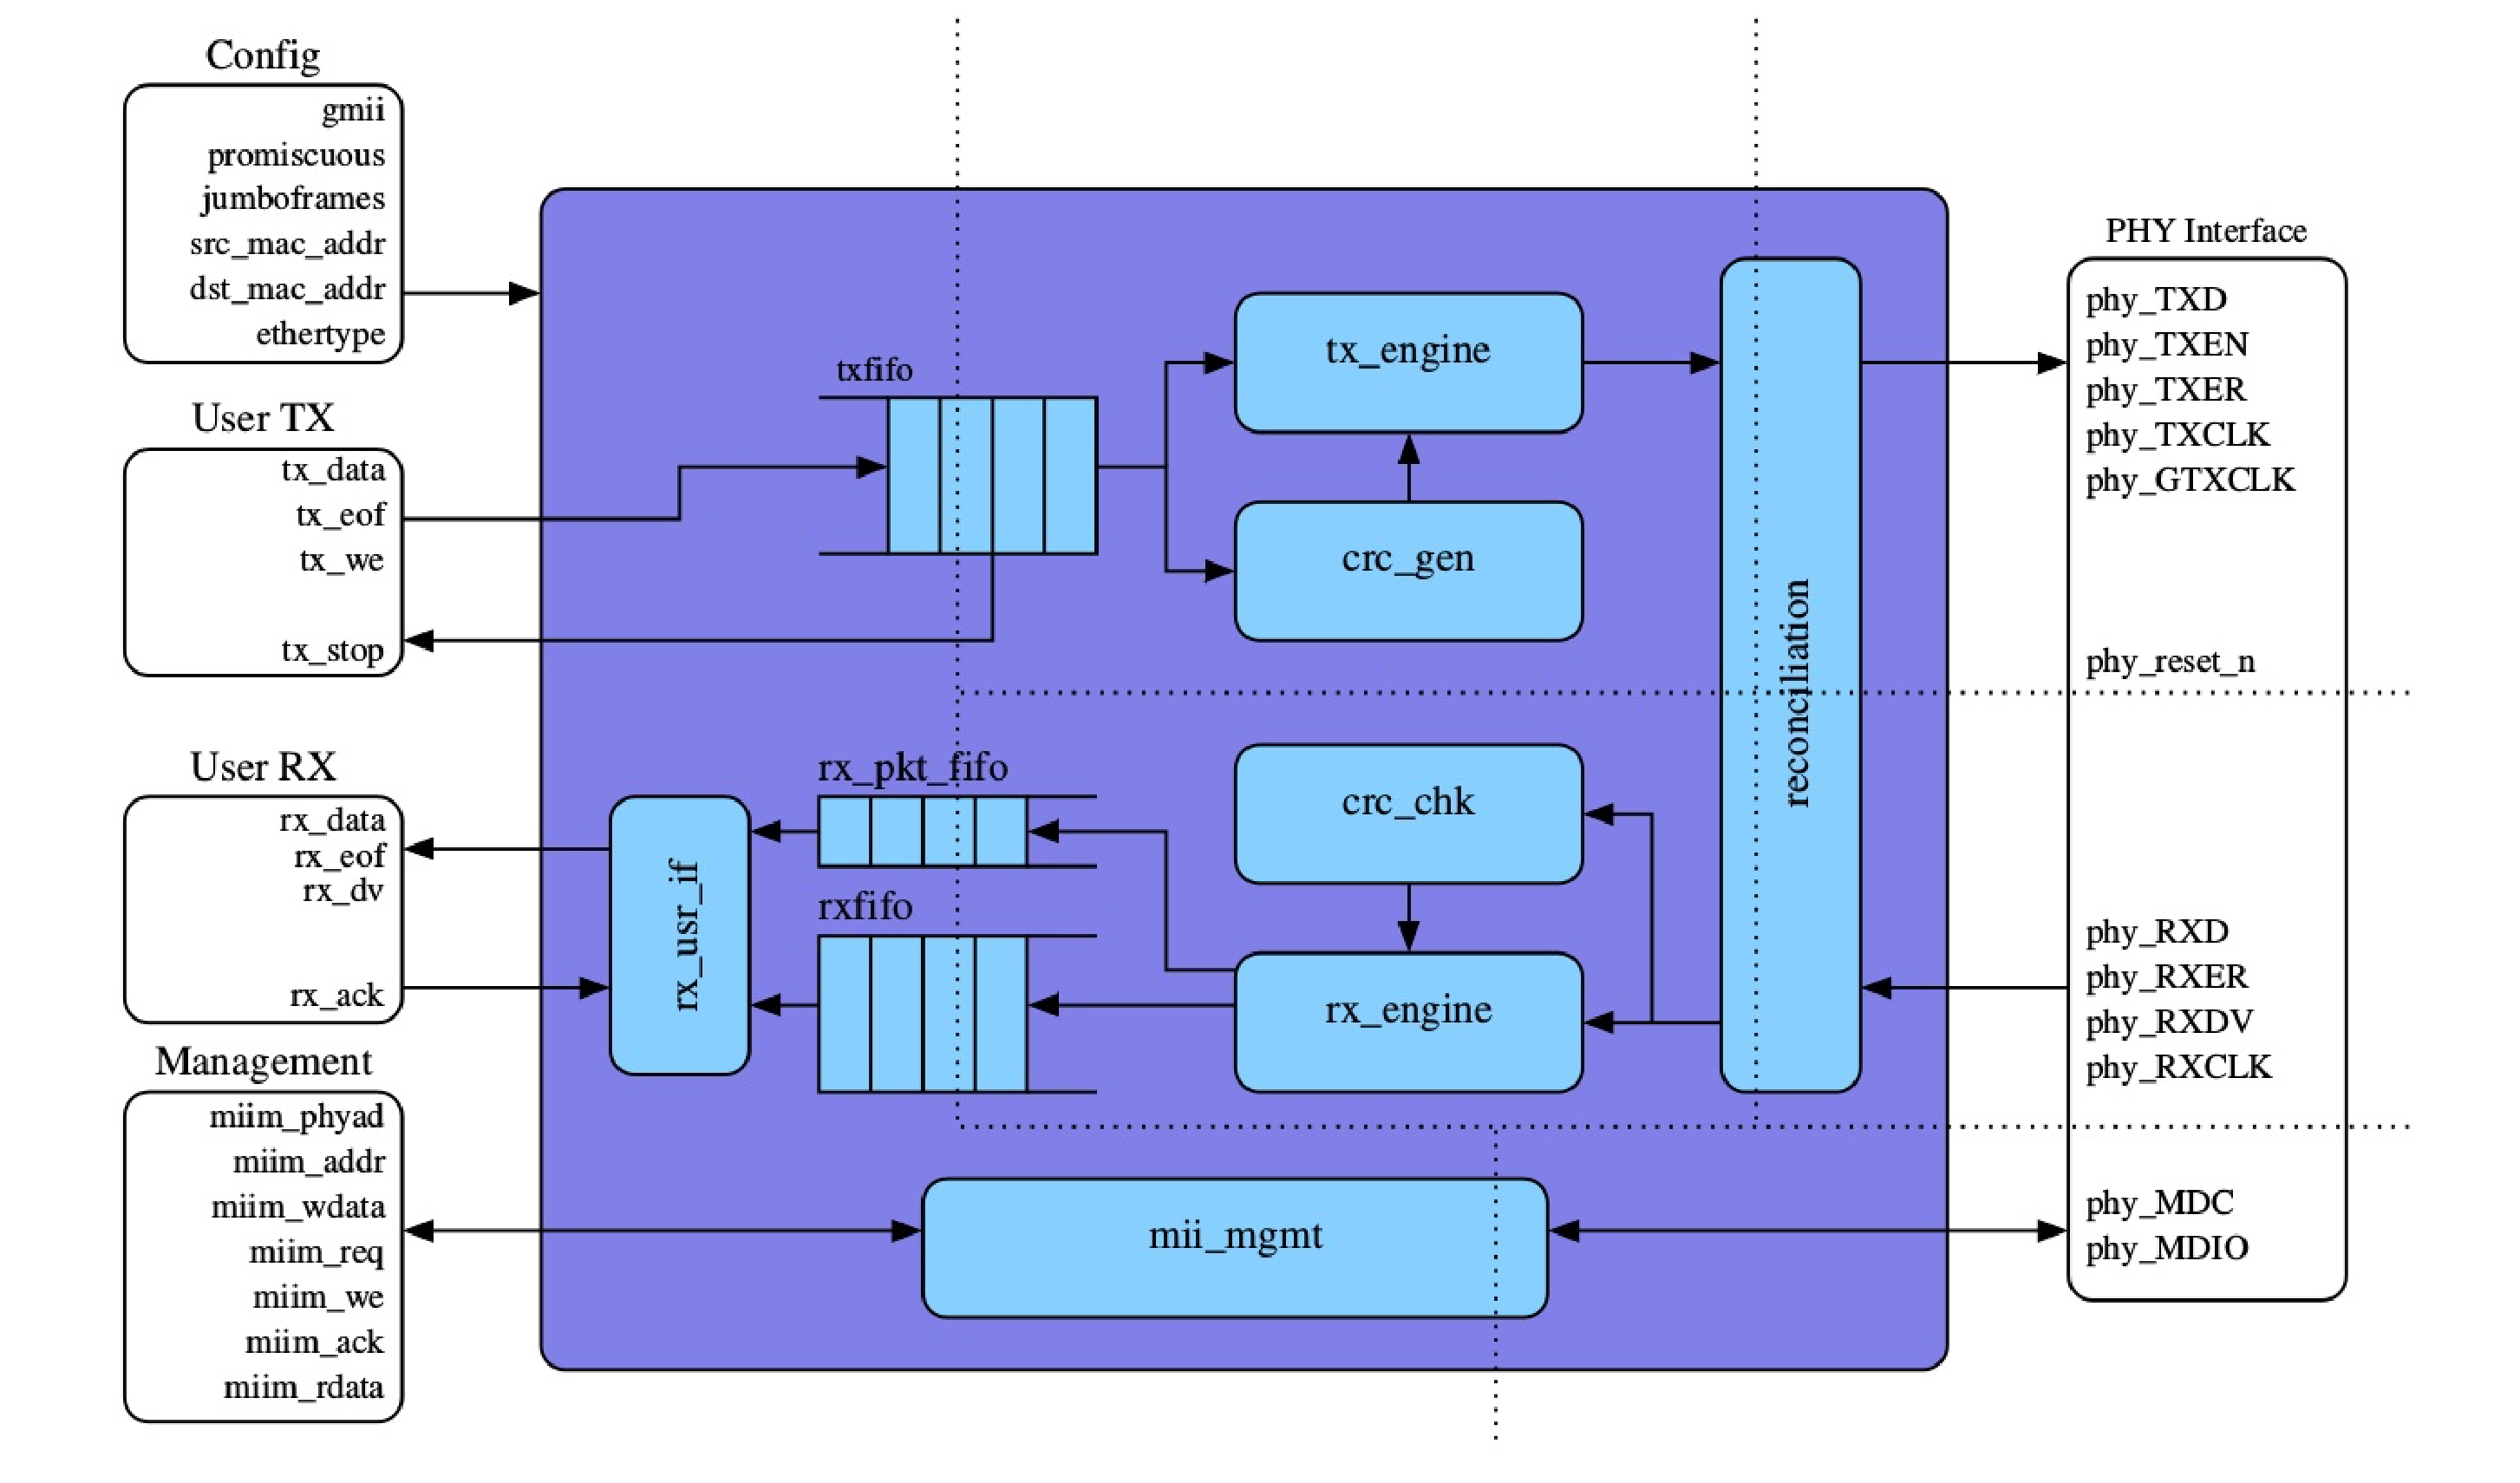
\includegraphics[scale=0.25]{eps/mac10.eps}
\caption{mac10}
\label{mac10}
\end{figure}

\end{enumerate}


\chapter{crcgen}

Here, we look into the $crc_gen.v$ code to see what it does.

\begin{chunk}{inoutputs}
  module $crc_gen$
  ( input clk, input reset_n,
    input init,
    input [7:0] data,
    input rden,
    output [7:0] crc);

\end{chunk}

\begin{enumerate}

\item inputs

clk--clock signal
$reset_n$--reset signal
init--initialization signal
data[7:0]--data array signal
rden--$control signal$

\item outputs

crc[7:0]--the crc array signal (cyclic redundancy check)



\end{enumerate}

\chapter{rxrawv}

Here, we look into the $rx_raw$ module.

\begin{chunk}{parameters}

#(parameter $CKSM_CHK$=1)

\end{chunk}

The parameters $rx_raw$ used are:

$CKSM_CHK$: From mac.v $RX_CKSM_CHECK$

\begin{chunk}{inoutputs}

(input $usr_clk$,
 input $reset_n$,

 // config
 input        promiscuous,
 input        jumboframes,
 input [47:0] $mac_addr_filter$,
 output [31:0] $rx_count$,

 // phy interface
 input       $int_rx_clk$,
 input [7:0] $int_rx_din$,
 input       $int_rx_dv$,
 input       $int_rx_er$,

 // user interface
 output [31:0] $rx_data$,
 output        $rx_sof$,
 output        $rx_dv$,
 input         $rx_ack$,

 output [17:0] debug);

\end{chunk}

The inoutputs are:

$usr_clk$: From mac.v, $usr_clk$
$reset_n$: From mac.v, $reset_n$

// config
promiscuous: From mac.v, promisuous
jumboframes: From mac.v, jumboframes
$mac_addr_filter$: From mac.v, $rx_raw_mac_addr$
$rx_count$: To mac.v, $rx_raw_count$

 // phy interface
$int_rx_clk$: From mac.v, $int_rx_clk$
$int_rx_din$: From mac.v, $int_rx_din$
$int_rx_dv$: From mac.v, $int_rx_dv$
$int_rx_er$: From mac.v, $int_rx_er$

 // user interface
$rx_data$: To mac.v, $rx_raw_data$
$rx_sof$: To mac.v, $rx_raw_sof$
$rx_dv$: To mac.v, $rx_raw_dv$
$rx_ack$: From mac.v, $rx_raw_ack$

debug: To mac.v, $rx_debug$

\begin{chunk}{crcgen}
$
wire crc_init;
wire [7:0] crc_data;
wire crc_good;
generate if (CKSM_CHK == 1) begin
   crc_chk U_crc_chk
     (.clk(int_rx_clk), .reset_n(reset_n), 
      .init(crc_init), .data(crc_data), .good(crc_good));
end
else begin
   assign crc_good = 1'b1;
end
endgenerate
$
\end{chunk}

this part of code send data to $crc_chk$ to generate the crc code for the data.
And the crc code is on $crc_good$

\begin{chunk}{rxpktfifo}
$
wire rfq_we;
wire [13:0] rfq_din;
wire rfq_ready;
wire rfq_dv;
wire [13:0] rfq_dout;
wire rfq_ack;
wire rfq_empty;
wire rfq_full;

rx_pkt_fifo U_rx_pkt_fifo
  (.reset_n(reset_n), .int_rx_clk(int_rx_clk), .usr_clk(usr_clk),
   .we(rfq_we), .din(rfq_din), .ready(rfq_ready),
   .dv(rfq_dv), .dout(rfq_dout), .ack(rfq_ack),
   .fifo_empty(rfq_empty), .fifo_full(rfq_full));
$
\end{chunk}

This part of code calls $rx_pkt_fifo$ to check if fifo is ready and could do what we want it to do.


\begin{chunk}{rxfifo}
$
wire [35:0] rxff_din;
wire rxff_we;
wire rxff_almost_full;
wire [35:0] rxff_dout;
wire rxff_empty;
wire rxff_ack;
wire rxff_full;
rxfifo U_rxfifo
  (.rst(~reset_n),
   .wr_clk(int_rx_clk), .din(rxff_din), .wr_en(rxff_we), 
   .full(rxff_full), .almost_full(rxff_almost_full),
   .rd_clk(usr_clk), .dout(rxff_dout), .rd_en(rxff_ack), .empty(rxff_empty));
$
\end{chunk}

This part of code calls for the wrapper $rxfifo.v$ from the coregen of spartan3e.

\begin{chunk}{rxengineraw}
$
rx_engine_raw U_rx_engine_raw
  (.clk(int_rx_clk), .reset_n(reset_n),
   .promiscuous(promiscuous), .jumboframes(jumboframes),
   .mac_addr_filter(mac_addr_filter), .rx_count(rx_count),
   .int_rx_din(int_rx_din), .int_rx_dv(int_rx_dv), .int_rx_er(int_rx_er),
   .crc_init(crc_init), .crc_data(crc_data), .crc_good(crc_good),
   .rxff_din(rxff_din), .rxff_we(rxff_we), .rxff_almost_full(rxff_almost_full),
   .rfq_din(rfq_din), .rfq_we(rfq_we), .rfq_ready(rfq_ready));
$
\end{chunk}

This part of code calls for $rx_engine_raw$ to 


\begin{chunk}{rxusrif}
$
rx_usr_if U_rx_usr_if
  (.clk(usr_clk), .reset_n(reset_n),
   .rxff_dout(rxff_dout), .rxff_empty(rxff_empty), .rxff_ack(rxff_ack),
   .rfq_dout(rfq_dout), .rfq_dv(rfq_dv), .rfq_ack(rfq_ack),
   .rx_data(rx_data), .rx_dv(rx_dv), .rx_sof(rx_sof), .rx_ack(rx_ack),
   .debug());
assign debug = { rfq_full, rfq_empty };
$
\end{chunk}

This part of code calls $rx_usr_if$ to 



\chapter{rxenginerawv}

$rx_engine_raw$ is part of the Reception blocks of MAC core.

\begin{chunk}{inoutputs}

(input clk, input $reset_n$,

 input        promiscuous,
 input        jumboframes,
 input [47:0] $mac_addr_filter$,
 output [31:0] $rx_count$,

 input [7:0] $int_rx_din$,
 input       $int_rx_dv$,
 input       $int_rx_er$,

 output       $crc_init$,
 output [7:0] $crc_data$,
 input        $crc_good$,

 output [35:0] $rxff_din$,
 output       $rxff_we$,
 input        $rxff_almost_full$,

 output [13:0] $rfq_din$,
 output        $rfq_we$,
 input         $rfq_ready$);

\end{chunk}


input: promiscuous is from configuration

input: jummboframs is from configuration

input: $mac_addr_filter$ is from configuration

input: $int_rx_din$, $int_rx_dv$ and $int_rx_er$ are from $reconciliation.v$

input: $crc_good$ from $crc_chk.v$






\chapter{macv}

Here, we look into the $mac.v$ code to see what it does.

\begin{chunk}{parameters}
$
  module mac
#(parameter USR_CLK_PERIOD=5,
  parameter RX_CKSM_CHECK=1,
  parameter RAW_TXIF_COUNT=1, 
  parameter RAW_RXIF_COUNT=1, 
  parameter STREAM_TXIF_COUNT=0,
  parameter STREAM_RXIF_COUNT=0) 
$
\end{chunk}

$USR_CLK_PERIOD:$
Period, in ns, of usr clk. Needed to to generate a sutable clock for the mii management port (mdc) from usr clk.



\begin{chunk}{inoutputs}
$
(input usr_clk, input clk_125, input reset_n,

 // config
 input        gmii,
 input        promiscuous,
 input        jumboframes,
 input [9:0]  ifg,

 // raw tx interface(s)
 input  [(RAW_TXIF_COUNT*32)-1:0] tx_raw_data,
 input  [RAW_TXIF_COUNT-1:0]      tx_raw_sof,
 input  [RAW_TXIF_COUNT-1:0]      tx_raw_we,
 output [RAW_TXIF_COUNT-1:0]      tx_raw_stop,
 output [(RAW_TXIF_COUNT*32)-1:0] tx_raw_count,

 // raw rx interface(s)
 input  [(RAW_RXIF_COUNT*48)-1:0] rx_raw_mac_addr,
 output [(RAW_RXIF_COUNT*32)-1:0] rx_raw_data,
 output [RAW_RXIF_COUNT-1:0]      rx_raw_sof,
 output [RAW_RXIF_COUNT-1:0]      rx_raw_dv,
 input  [RAW_RXIF_COUNT-1:0]      rx_raw_ack,
 output [(RAW_RXIF_COUNT*32)-1:0] rx_raw_count,
 
 // management interface
 input [0:4]   miim_phyad,
 input [0:4]   miim_addr,
 input [0:15]  miim_wdata,
 input         miim_req,
 input         miim_we,
 output        miim_ack,
 output [15:0] miim_rdata,    

 // PHY interface
 output [7:0] phy_TXD,
 output       phy_TXEN,
 output       phy_GTXCLK,
 output       phy_TXER,
 input        phy_TXCLK,
 input        phy_RXCLK,
 input [7:0]  phy_RXD,
 input        phy_RXER,
 input        phy_RXDV,
 output       phy_RESET_N,

 output       phy_MDC,
 inout        phy_MDIO,

 output [31:0] debug);
$
\end{chunk}



\chapter{MACworkflow}

\begin{figure}[ht!]
\centering
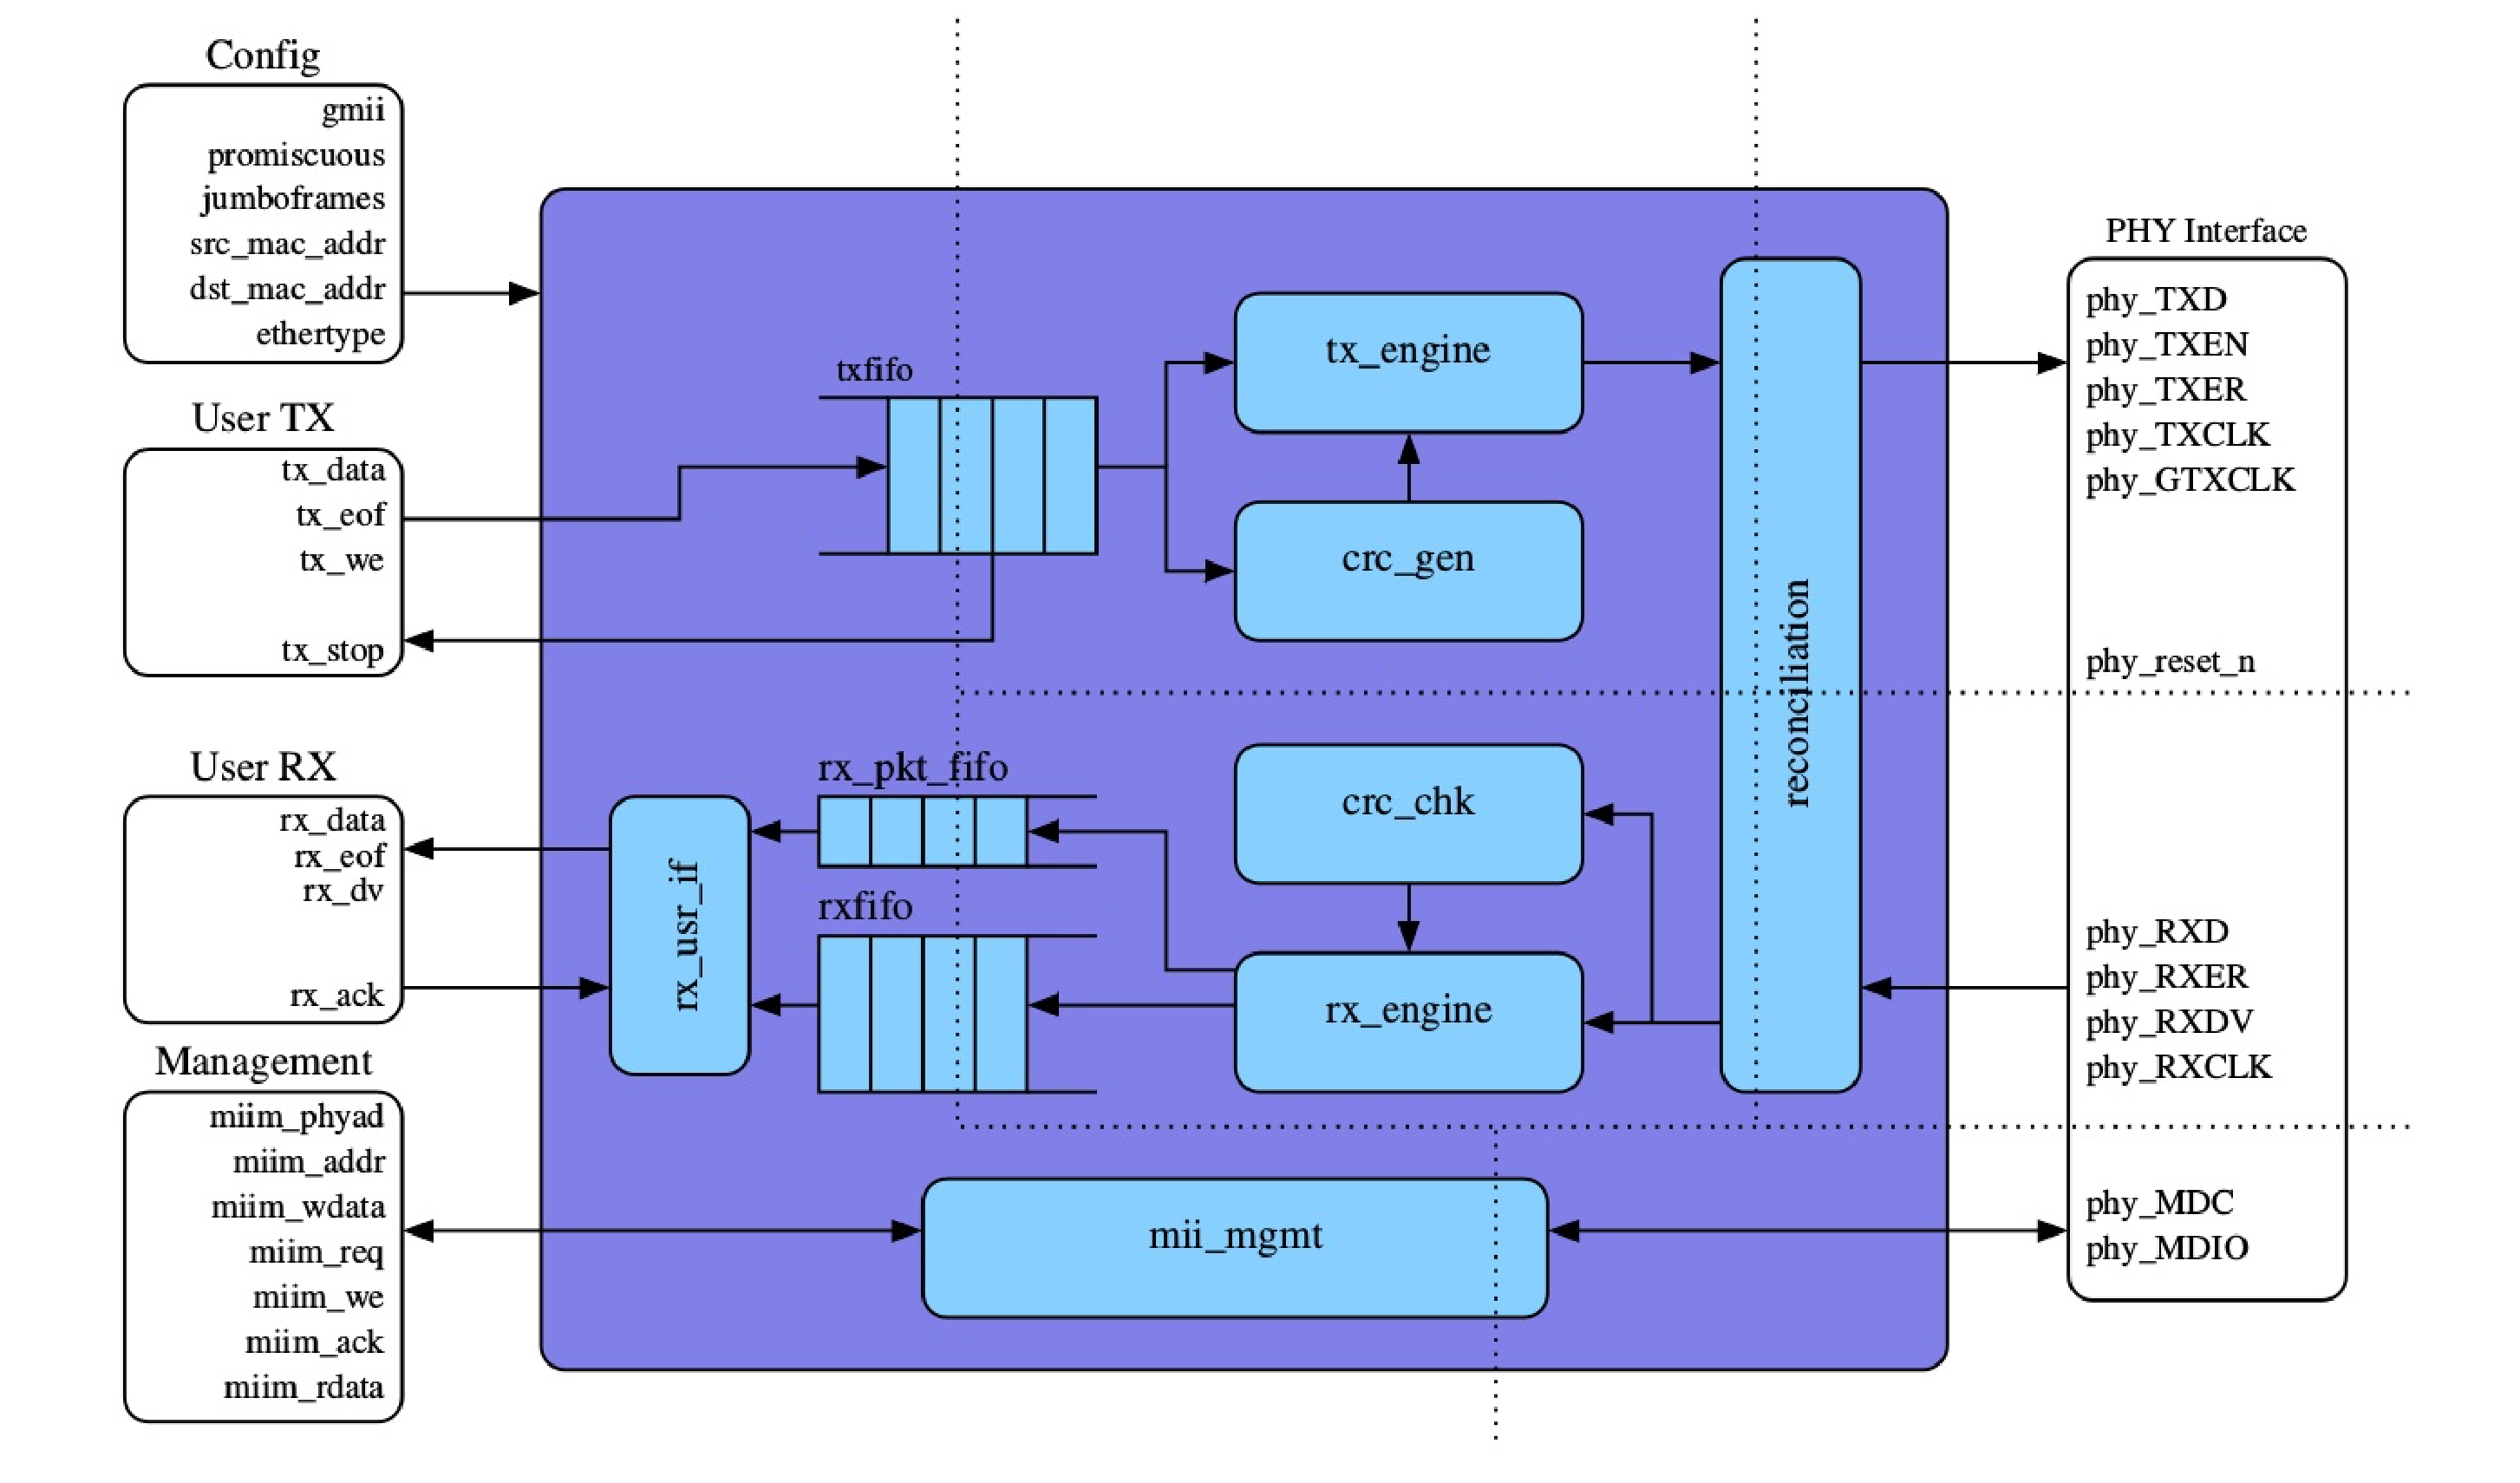
\includegraphics[scale=0.25]{eps/mac10.eps}
\caption{The mac10}
\label{mac10}
\end{figure}

This is the block diagram of the MAC core, which is very important in understanding how the MAC functions.

From the MAC chapter, we know that the MAC mainly has three parts: reception, reconciliation, and transmission.

The transmission part includes txfifo, $tx_engine$, and $crc_gen$, which takes the user data and send it to reconciliation module, which send it to ethernet phy.

The reception part includes $rx_usr_if$, $rx_pkt_fifo$, $rxfifo$, $rx_engine$, and $crc_chk$, which takes data from reconciliation, throwing away bad frames, and then present them to the user

The reconciliation part deals with GMII interface to phy.

TO use the MAC core, we can simply implement the configuration ports that MAC presents to us, which is listed and explained as follows:

gmii: a flag that indicates whether the MAC core should be communicate with the phy in GMII mode or MII mode.

promiscous: a flag that indicates the MAC core should filter incoming packages to those with destination of $src_mac_addr$

$src_mac_addr$: this is the MAC address to use as the source of transmitted ethernet frames and the filter for what received frames to not discard when not in promiscous mode

$dst_mac_addr$: this is the MAC address to use as the destination of transmitted ethernet frames.

ethertype: the EtherType/Length field for outgoing packets

ifg: this is the number of cycles inserted between packets, should be $>= 0x0D$





\chapter{reconciliation}

Here we look into the reconciliation layer, which deals with all the differences between MII and GMII (and eventually RGMII).

\begin{chunk}{inoutputs}

$
module reconciliation
(input clk_125, input reset_n,
 
 // decides whether we are in gmii or mii mode
 input gmii,

 input [7:0] int_tx_dout,
 input int_tx_en,
 input int_tx_er,
 output int_tx_clk,

 output [7:0] int_rx_din,
 output int_rx_dv,
 output int_rx_er,
 output int_rx_clk,
 
 output [7:0] phy_TXD,
 output       phy_TXEN,
 output       phy_TXER,
 output       phy_GTXCLK,
 input        phy_TXCLK,
 input  [7:0] phy_RXD,
 input        phy_RXDV,
 input        phy_RXER,
 input        phy_RXCLK
 );	
$

\end{chunk}

\begin{enumerate}
\item Transmission

Generate $int_tx_clk$, which is what the mac is clocking data in on,
and $tx_clk$ which is what we are clocking data out on. If we are in
MII mode, we ship 4 bits every $phy_TXCLK$, so we want the mac to
clock the data in every other $phy_TXCLK$ since the mac interface is
8 bits.  We divide $phy_TXCLK$ by two and send that as the
$int_tx_clk$.  Otherwise, we are in GMII mode and sending 8 bits
every $phy_GTXCLK$, so send the full $phy_GTXCLK$ as $int_tx_clk$.

\begin{chunk}{transmiss}
$
wire mii_tx_clk;
greg mtc_reg(phy_TXCLK, ~mii_tx_clk, 1'b0, ~reset_n, 1'b1, mii_tx_clk);
BUFGMUX int_tx_clk_mux(.O(int_tx_clk), .I0(mii_tx_clk), .I1(clk_125), .S(gmii));

// Now generate tx_clk, which is used to clock the data out, this is
// simply clk_125 if gmii or phy_TXCLK if not.

wire tx_clk;
// BUFGMUX tx_clk_mux(.O(tx_clk), .I0(phy_TXCLK), .I1(clk_125), .S(gmii));
assign tx_clk = phy_TXCLK;


// Generate the output GTX clock to the phy, this will only be used in
// gmii mode.  We use an ODDR to delay and flip the clock so that
// the rising edge is sent in the middle of the data (sent below)
wire tmp0 = 1'b0;
wire tmp1 = 1'b1;
device_ODDR gtx_clk_out(.S(tmp0), .R(tmp0), .CE(tmp1), 
                        .D0(1'b0), .C0(tx_clk), .D1(1'b1), .C1(~tx_clk), 
                        .Q(phy_GTXCLK));

// now deal with the data.  For mii we alternate between nibbles.  For
// gmii we just blast the whole int_tx_dout each clock.
wire mii_tx_sel;
greg mts_reg(tx_clk, ~mii_tx_sel, ~int_tx_en, ~reset_n, 1'b1, mii_tx_sel);

wire [3:0] mii_txd;
gmux #(4, 1) mii_txd_mux(.d(int_tx_dout), .sel(mii_tx_sel), .z(mii_txd));

wire [7:0] next_txd;
gmux #(8, 1) txd_sel(.d({int_tx_dout, 4'h0, mii_txd}), .sel(gmii), .z(next_txd));

// TODO crossing clock domains... metastability??  Should be in phase...

greg #(8) TXD_reg(tx_clk, next_txd, 1'b0, ~reset_n, 1'b1, phy_TXD);
greg #(1) TXEN_reg(tx_clk, int_tx_en, 1'b0, ~reset_n, 1'b1, phy_TXEN);
greg #(1) TXER_reg(tx_clk, int_tx_er, 1'b0, ~reset_n, 1'b1, phy_TXER);
$
\end{chunk}

\item Reception

Again deal with the clocks first.  If we are in MII mode, the phy
sends 4 bits every $phy_RXCLK$, so the mac should be running at half
$phy_RXCLK$ to get 8 bits each clock tick.  If we are in GMII mode,
the phy sends 8 bits every $phy_RXCLK$, so we can just send the
clock directly through.

\begin{chunk}{receptio}
$
wire mii_rx_clk;
greg rcc_reg(phy_RXCLK, ~mii_rx_clk, 1'b0, ~reset_n, 1'b1, mii_rx_clk);
BUFGMUX int_rx_clk_mux(.O(int_rx_clk), .I0(mii_rx_clk), .I1(phy_RXCLK), .S(gmii));

// the data is a bit harder.  We start by registering the signals
// coming in the from the phy
wire [7:0] rx_din_0;
wire [3:0] rx_din_1;
wire rx_dv_0, rx_dv_1;
wire rx_er_0, rx_er_1;
greg #(8) rx_din_r0(phy_RXCLK, phy_RXD, 1'b0, ~reset_n, 1'b1, rx_din_0);
greg #(1) rx_dv_r0(phy_RXCLK, phy_RXDV, 1'b0, ~reset_n, 1'b1, rx_dv_0);
greg #(1) rx_er_r0(phy_RXCLK, phy_RXER, 1'b0, ~reset_n, 1'b1, rx_er_0);
$
\end{chunk}

the above signal are fine for gmii, but for mii, we need to hold
them for two $phy_RXCLK$ cycles, and not just any two, a cycle with
$int_rx_clk$ low and a cycle with $int_rx_clk$ high. So we want to
bring a new value in when $int_rx_clk$ is high.  To know what delay
registers to use, we sample it when $phy_RXDV$ goes high indicating
a new frame.  If $int_rx_clk$ is high on $new_frame$ is high, $rx_din$
will be get it's first nibble when $int_rx_clk$ is low.


\begin{chunk}{recept2}
$
wire new_frame = ~rx_dv_0 & phy_RXDV;
wire started_on_low;
greg #(1) sol_reg(phy_RXCLK, mii_rx_clk, 1'b0, ~reset_n, new_frame, started_on_low);

greg #(4) rx_din_r1(phy_RXCLK, rx_din_0[3:0], 1'b0, ~reset_n, 1'b1, rx_din_1);
greg #(1) rx_dv_r1(phy_RXCLK, rx_dv_0, 1'b0, ~reset_n, 1'b1, rx_dv_1);
greg #(1) rx_er_r1(phy_RXCLK, rx_er_0, 1'b0, ~reset_n, 1'b1, rx_er_1);

wire [7:0] next_mii_rx_din;
wire next_mii_rx_dv;
wire next_mii_rx_er;
gmux #(10, 1) mii_rx_din_mux
  (.d({phy_RXER, phy_RXDV & ~new_frame, phy_RXD[3:0], rx_din_0[3:0],
       rx_er_1, rx_dv_1, rx_din_0[3:0], rx_din_1[3:0]}),
   .sel(started_on_low),
   .z({next_mii_rx_er, next_mii_rx_dv, next_mii_rx_din}));

wire [7:0] mii_rx_din; 
wire mii_rx_dv;
wire mii_rx_er;
greg #(8) mii_rx_din_r1(phy_RXCLK, next_mii_rx_din, 1'b0, ~reset_n, ~mii_rx_clk, mii_rx_din);
greg #(1) mii_rx_dv_r1(phy_RXCLK, next_mii_rx_dv, 1'b0, ~reset_n, ~mii_rx_clk, mii_rx_dv);
greg #(1) mii_rx_er_r1(phy_RXCLK, next_mii_rx_er, 1'b0, ~reset_n, ~mii_rx_clk, mii_rx_er);

wire [7:0] next_int_rx_din;
wire next_int_rx_dv;
wire next_int_rx_er;
gmux #(10, 1) rx_mux
  (.d({rx_er_0, rx_dv_0, rx_din_0, mii_rx_er, mii_rx_dv, mii_rx_din}),
   .sel(gmii),
   .z({next_int_rx_er, next_int_rx_dv, next_int_rx_din}));

greg #(8) int_rx_din_reg(phy_RXCLK, next_int_rx_din, 1'b0, ~reset_n, 1'b1, int_rx_din);
greg #(1) int_rx_dv_reg(phy_RXCLK, next_int_rx_dv, 1'b0, ~reset_n, 1'b1, int_rx_dv); 
greg #(1) int_rx_er_reg(phy_RXCLK, next_int_rx_er, 1'b0, ~reset_n, 1'b1, int_rx_er);

endmodule
$
\end{chunk}

register the output of all this craziness to maintain 125 MHz these
registers act as the cross from the $phy_RXCLK$ domain to the
$int_rx_clk$ domain.  TODO $-$ metastability issues.

\end{enumerate}

\chapter{J1 Forth Level Network Code}
The J1 cpu runs the programming language Forth. The file {\bf basewords.fs}
defines the forth words in terms of the J1 hardware.

\section{English for forth programmers \cite{64}}

There is a difference between spelling a word and saying a word.  In
normal communication we do not ess-pee-ee-ell-ell words.  Likewise we
do not normally pronounce punctuation.  (Period.)  Sometimes it is
necessary to spell for complete understanding but comprehension is
generally easier when natural language is spoken.

A language may also have special signs \verb|&| symbols which are normally
``said'', e.g., ``\verb|&|'' and ``\verb|#|'' are normally pronounced
``and'' and ``number''.  Spelling often has very little relationship to
the pronunciation, e.g., ``lb'' is ``pound'' and ``cwt'' is ``hundredweight''.

Forth is a language of natural English words and signs using
machine  oriented  syntax for command and control of machines.

The so-called natural pronunciation of Forth words given in the
Forth-79 and Forth-83 standard documents are mostly spellings.
Experience has shown that Forth programs are easier to teach and
understand when natural English words are used for the special signs.

An obvious example of this is ``\verb|#|''.  The standard documents
give  ``sharp''  as  its natural pronunciation.  This is patently
wrong.  The musical sharp sign is similar to it but  different.
The semantics of all occurrences of ``\verb|#|'' in standard Forth words
are connected with numbers.  ``\verb|#|'' should be  said  ``number''  and
spelled ``number-sign''.

The standard specification of ``\verb|@|'' is ``value at $<$address$>$''.
It makes more sense to say ``value'' than ``fetch''  when  we  read
it.   Likewise  ``!''  reads  better  as ``set'', which is what the
function is called in other high-level  languages.   E.g.,  the
body of the definition of ``DEFINITIONS''
\begin{verbatim}
          CURRENT @ CONTEXT !
\end{verbatim}

reads naturally as
\begin{verbatim}
          current value context set
\end{verbatim}

This says What it does, not How it does it.  This  agrees  with
the  Forth-83  standard document, which says that ``descriptive''
names are to be preferred to ``procedural'' names (section 4).

Reflection leads to ``add''  as  the  meaning  of  ``\verb|+!|''.   A
fragment of code
\begin{verbatim}
          0 #LINE !   1 #PAGE +!
\end{verbatim}

reads naturally as
\begin{verbatim}
          zero number-line set   one number-page add
\end{verbatim}

The so-called natural pronunciation of the apostrophe  ``'''
is   given   as  ``tick''  in  the  Forth-83  standard  document,
ignoring  descriptive and procedural names.  A better word  for
this is ``address''.  This also works well in compounds: from the
Perry Line-Editor read
\begin{verbatim}
     'START   'LINE   'CURSOR   'FIND
\end{verbatim}

as
\begin{verbatim}
     address-start  address-line  address-cursor  address-find
\end{verbatim}

``compile-time-address''  is a better name for  ``[']''.   In
general say ``compile-time-name'' for ``[name]''.

The function  of  the  dot  or  period  ``.''  in  Forth  is
``display''.   The  Forth  word  spelled  ``dot-quote''  is used to
display a message; the Forth word spelled ``ABORT-quote'' is used
to abort with a message.  They should be said ``display-message''
and ``abort-message'', which are perfect descriptions.

Forth has three  common  conventions  for  names  within parentheses.

``(name)'' is the default value of a vectored word.  E.g.,
\begin{verbatim}
          (CR)   (KEY)
\end{verbatim}

``(name)'' is used by ``name''.  E.g.,
\begin{verbatim}
          (.)
\end{verbatim}

``(name)'' is compiled by ``name''.  E.g.,
\begin{verbatim}
          (.'')   (ABORT'')   (LOOP)
\end{verbatim}

Notice that the third case is a subset of the second.

All these uses can be covered by ``primitive''.
\begin{verbatim}
     (CR)          primitive CR
     (KEY)         primitive key
     (.)           primitive display
     (.'')          primitive display message
     (ABORT'')      primitive abort message
     (LOOP)        primitive loop
\end{verbatim}

``,''  is  used to lay down values in the dictionary, and we
say ``lay'' or ``lay down'' or ``build'' for this function.

Just  as  Forth  is  said  to  have  been  discovered, not
invented, so the foregoing words were discovered in  the  order
given.  Having come so far, we would like to go the rest of the
way.

``[`` is used to initiate interpretation, but ``INTERPRET'' is
a word in the controlled word-set.  We pronounce it ``evaluate''.

A stumbling stone in  learning  Forth  is  the  difference
between ``]'', ``COMPILE'', and ``[COMPILE]''.

If  we  think  of  ``]''  as  ``construct''  we  have a way to
distinquish ``]'' from the other two.  ``COMPILE'' will ``compile'' a
defined word into the dictionary;   ``]''  will  do  whatever  is
necessary  to  ``construct''  the  dictionary,  including defined
words, literal values, logical structures, and anything else.

``[COMPILE]''  is  ``compile-time  compile'',  which  accurately
describes  what it does, compile the next word as a single word
at compile-time, not run-time.

Some examples to show how this hangs together.

\begin{verbatim}
     : ASCII  ( -- c ) BL WORD COUNT 1- ABORT'' ?''
        STATE @ IF [COMPILE] LITERAL THEN ; IMMEDIATE
\end{verbatim}

``Define   ASCII  BL  word  count  one-minus  abort-message
question-mark  state   value   if  compile-time-compile literal
then.  Immediate.''

Note that punctuation  was  not  pronounced.   Punctuation
can be spelled when necessary for comprehension.

From  the  preceding  paragraph  we  see how ``(`` should be
pronounced, i.e., ``note''.  Likewise ``.(`` is ``display-note''.

From an integer-ascii conversion definition:

\begin{verbatim}
     ... [ ASCII A 10 - ] LITERAL ...

     ``... evaluate ascii A 10 minus construct literal ...''
\end{verbatim}

The prefix ``C'' is  used  in  Forth  to  show  byte-related
operations.   Just  as  ``cwt''  is pronounced ``hundredweight'' so
``\verb|C@|'', ``C!'',  and  ``C,''  have  the  pronunciation  ``byte-value'',
``byte-set'', and ``byte-lay(down)''.

How about ``possibly'' or ``maybe'' for the question mark when
it is part of a word, e.g., ``maybe DUP'' for ``?DUP'' ?

We  can say ``define'' for ``:'' as we did above.  The ``;'' can
be silent punctuation, or we can use the  Eastern  ``already'' or
Western  ``y'know''  until some-one has a better suggestion.

Here  is  a  summary of the suggested pronunciations. 
\begin{verbatim}
     #               number
     @               value
     !               set
     +!              add
     '               address
     [']             compile-time address
     .               display
     .''              display message
     ABORT''          abort message
     (name)          primitive name
     ,               lay down, or lay
     [               evaluate
     ]               construct
     [COMPILE]       compile-time compile
     (               note
     .(              display note
     ?...            maybe ..., or possibly ...
     :               define
     ;               already, or y'know.
\end{verbatim}

The file {\bf nuc.fs} implements the standard words from the Forth
standard \cite{64} so that the standard words work.

For example, the Forth standard defines the standard word \verb|C@| as
\begin{verbatim}
6.1.0870   C@ ``c-fetch'' CORE
  ( c-addr -- char )
 Fetch the character stored at c-addr.  When the cell size is greater
 than character size, the unused high-order bits are all zeroes.
\end{verbatim}

whereas {\bf nuc.fs} implements this on the J1 as:
\begin{verbatim}
: c@    dup @ swap d# 1 and if d# 8 rshift else d# 255 and then ;
\end{verbatim}

\section{Connecting to the Hardware}

We need to connect the port assignments in the verilog, such as in
the file topj1.v, to the constants used in the forth code. The forth
constants are in the ile hwwge.fs. So, for instance, the constant
6010 in topj1.v is identical to the name \verb|rx_mac_filter| in hwwge.fs.

Next the bootstrap loader {\bf boot.fs} loads the system from flash.

The {\bf nuc.fs} file, mentioned above, implements standard forth words
on the J1.

The {\bf mac.fs} file contains the {\bf mac-cold} word which handles
reset of the MII device.

The {\bf morse.fs} file, when loaded, causes the LEDs to flash morse code.
There are 5 morse letters, (A, H, O, S, V) which mark the current state
of the process.
\begin{itemize}
\item A means the mac interface is ready for the next 32 bits.
\item S is the sleep state
\item V is the vertical blank state of the camera
\end{itemize}
The alarms and sleep handling are in {\b time.fs}

The routine {\bf mac-cold} in {\bf mac.fs} resets the MAC interface.

The file {\bf continuation.fs} handles saving and restoring program state.

The file {\bf packet.fs} contains the words to handle packet construction,
transmission, and reception.

The file {\bf ip0.fs} initializes variables for the ip-address, 
subnet mask, dns, etc.

The file {\bf defines\_tcpip.fs} contains constants defining the
offsets for various parts of a packet.

The file {\bf defines\_tcpip2.fs} contains constants defining the
offsets for ethernet packets.

The file {\bf arp.fs} sets up and manages the arp cache.

The file {\bf ip.fs} handles IP ping/response, UDP checksums,
and ICMP packets.

The file {\bf dhcp.fs} handles DHCP packets and leases.

The file {\bf spi.fs} handles the serial peripheral interface.

The file {\bf flash.fs} handles flash memory.

The file {\bf mt9v.fs} is the hardware interface for camera.

The file {\bf wge.fs} handles the Willow Garage Ethernet camera protocol.

The file {\bf newtcp.fs} handles low level TCP words.

The file {\bf html.fs} constructs an HTML page

The file {\bf http.fs} implements the HTTP protocol

The file {\bf tcpservice.fs} handles the TCP general service scheme.

The file {\bf ntp.fs} handles the network time protocol.

The file {\bf syslog.fs} implements a syslog (RFC 5424)

The file {\bf epa.fs} implements arbitrary precision arithmetic,
along with the file {\bf reference\_epa.fs}.

The file {\bf i2c} handles the i2c serial interface.

The file {\bf rate.fs} is a rate reporting tool.

The file {\bf testmt9v.fs} is a self-test tool for the camera.

The file {\bf go} is a shell script to start the system.

\section{main.fs}
\begin{verbatim}
( Main for WGE firmware                      JCB 13:24 08/24/10)

\ warnings off require tags.fs

include crossj1.fs
meta
    : TARGET? 1 ;
    : ONBENCH 0 ;
    : SYSLOG 0 ;
    : DO-XORLINE 1 ;
    : build-debug? 1 ;
    : build-tcp? 0 ;

include basewords.fs
target
include hwwge.fs
include boot.fs
include doc.fs

4 org
module[ eveything"
include nuc.fs

create mac         6 allot
create serial      4 allot
create camera_name 40 allot

: net-my-mac mac dup @ swap 2+ dup @ swap 2+ @ ;

: halt  [char] # emit begin again ;

: alarm
    s" ** failed selftest: code " type hex2 cr
    halt
;

include version.fs
include parseversion.fs

: rapidflash
    time 2+ @ led ! ;
: morseflash ( code -- )
    time 2+ @ 2/ h# f and rshift invert led ! ;

include morse.fs
include time.fs
include mac.fs
include continuation.fs
include packet.fs
include ip0.fs
include defines_tcpip.fs
include defines_tcpip2.fs
include arp.fs
include ip.fs
include dhcp.fs

include spi.fs
include flash.fs

: hardreset 
    true trig_reconf ! begin again ;

: softreset
    ['] emit-uart is emit
    sleep1 [char] a emit cr sleep1
    begin dsp h# ff and while drop repeat
    begin dsp d# 8 rshift while r> drop repeat
    dsp hex4 cr
    d# 0 >r
    sleep1 [char] b emit cr sleep1
;

include mt9v.fs

: setrouter ( router subnet -- )
    ip-subnetmask 2! ip-router 2!
    arp-reset
    net-my-ip arp-lookup drop arp-announce ;

: guess-mask ( ip -- )
    ip# 0.0.0.0 \ the world is my LAN
    ip# 0.0.0.0
    setrouter

    ip# 255.255.0.0 dand
    2dup ip# 10.0.0.0 d= if
        ip# 10.0.0.1 
        ip# 255.255.248.0 
        setrouter
    then
    2dup ip# 10.68.0.0 d= if
        ip# 10.68.0.1 
        ip# 255.255.255.0 
        setrouter
    then
    ip# 10.69.0.0 d= if
        ip# 10.69.0.11
        ip# 255.255.255.0 
        setrouter
    then
;

: ip-addr! ( ip -- )
    2dup ip-addr 2@ d<> if
        2dup ip-addr 2!
        guess-mask
        arp-reset
    else
        2drop
    then
;

include wge.fs
build-tcp? [IF]
    include newtcp.fs
    include html.fs
    include http.fs
    include tcpservice.fs
[THEN]


( IP address formatting                      JCB 14:50 10/26/10)

: #ip1  h# ff and s>d #s 2drop ;
: #.    [char] . hold ;
: #ip2  dup #ip1 #. d# 8 rshift #ip1 ;
: #ip   ( ip -- c-addr u) dup #ip2 #. over #ip2 ;

( net-watchdog                               JCB 09:26 10/13/10)

2variable net-watchdog
: net-watch-reset
    d# 10000000. net-watchdog setalarm ;
: net-watch-expired?
    net-watchdog isalarm ;

: preip-handler
    begin
        enc-fullness
    while
        OFFSET_ETH_TYPE packet@ h# 800 =
        if
           dhcp-wait-offer
        then
        camera-handler
    repeat
;

: strlen ( addr -- u ) dup begin count 0= until swap - 1- ;

include ntp.fs

: haveip-handler
    begin
        enc-fullness
    while
        net-watch-reset
        arp-handler
        OFFSET_ETH_TYPE packet@ h# 800 =
        if
            d# 2 OFFSET_IP_DSTIP enc-offset enc@n net-my-ip d=
            if
                icmp-handler
                \ IP_PROTO_TCP ip-isproto if servetcp then
                \ ntp-handler
            then
            camera-handler
        then
        depth if .s cr then
        depth d# 6 u> if hardreset then
    repeat
;

: bench   
    cbench
    d# 1000 >r \ iterations
    time@
    r@ negate begin
        \ d# 33. d# 101. 2d+ drop drop
        \ d# 33 d# 101 +1c drop
        \ d# 23 s>q d# 11 d# 17 qm*/ qdrop
        progress

        d# 1 + dup d# 0 =
    until drop
    time@
    decimal s" bench: " type
    2swap d- d# 6800 r> m*/ d# 600. d- <# # # [char] . hold #s #> type
    s"  cycles" type cr
;

ONBENCH [IF]
    : banner
        cr cr
        d# 64 0do [char] * emit loop cr
        s" J1 running" type cr
        cr

        s" Imager:  " type imagerversion @ hex4 cr
        s" PCB rev: " type pcb_rev @ . cr
        s" HDL rev: " type hdl_version @ hex4 cr
        s" FW rev:  " type version type
            s"  reports as " type version version-n hex d. decimal cr
        s" serial:  " type serial 2@ d. cr
        s" MAC:     " type net-my-mac mac-pretty cr
        cr
    ;
    : phy-report s" PHY status: " type d# 1 mac-mii@ hex4 cr ;

    create prev d# 4 allot
    : clocker
        time@ prev 2@ d- d# 1000000. d> if
            time@ prev 2!
            time@ hex8 space
            cr

            \ ntp-server arp-lookup if ntp-request then
        then
    ;
[ELSE]
    : phy-report ;
[THEN]

: .mii ( reg -- ) \ print MII reg value
    s" PHY" type dup . mac-mii@ hex4 ;

0 constant MIICONTROL
1 constant MIISTATUS
27 constant SPECIALS

: hackit
    \ MAC seems to need a long reset
    d# 0 MAC_reset ! sleep.1 d# 1 MAC_reset ! sleep.1
    \ Turn off auto-neg
    
    begin
         \ Register 0, Bit 12  = 0
         \ Register 0, Bit 13 = 1
         \  Register 0, Bit 8 = 1
        MIICONTROL mac-mii@
            h# efff and
            h# 2100 or
        snap MIICONTROL mac-mii!
        snap
        h# 8000 SPECIALS mac-mii!
        snap
        MIICONTROL .mii space MIISTATUS .mii space SPECIALS .mii cr
        sleep1
    again
;

SYSLOG [IF]
include syslog.fs
[THEN]

: get-dhcp
    net-my-mac xor mt9v-random d+ dhcp-xid!
    d# 0. dhcp-alarm setalarm

    d# 1000
    begin
        net-my-ip d0=
    while
        dhcp-alarm isalarm if
            dhcp-discover
            2* d# 8000 min
            dup d# 1000 m* dhcp-alarm setalarm
        then
        preip-handler
    repeat
    snap
    drop
    depth if begin again then
;

2variable ntp-alarm

: silence drop ;

: main
    decimal
    mt9v-cold
    atmel-cold
    atmel-cfg-rd
    atmel-id-rd

    ONBENCH [IF]
        banner
    [THEN]

    \ hackit

    net-my-mac mac-cold
    phy-report

    net-my-ip d0= if
        get-dhcp
    else
        net-my-ip guess-mask
    then

    arp-reset

    build-tcp? [IF]
        tcp-cold
    [THEN]

    ONBENCH [IF]
        dhcp-status
    [THEN]
    SYSLOG [IF]
        begin
            haveip-handler syslog-server arp-lookup 0=
        while
            sleep.1
        repeat
        s" syslog -> " type syslog-server ip-pretty cr 
        syslog-cold ['] emit-syslog is emit
    [ELSE]
        ['] silence is emit
    [THEN]

    build-debug? [IF]
        s" booted serial://" type serial 2@ d.
        s" from " type
        h# 3ffe @ if s" mcs" else s" flash" then type
        s"  ip " type
        net-my-ip <# #ip #> type space
        s" xorline=" type
        [ DO-XORLINE ] literal hex1 space
        version type
        cr
        s" ready" type cr
    [THEN]

    \ net-my-ip arp-lookup drop arp-announce

    d# 1000000. ntp-alarm setalarm
    net-watch-reset
    begin
        \ clocker
        inframe invert if
            haveip-handler
        then
        mt9v-cycle
        net-watch-expired? if
            net-watch-reset
            mt9v-cold
            net-my-mac mac-cold
        then
        \ ntp-alarm isalarm if
        \     ntp-request
        \     d# 1000000. ntp-alarm setalarm
        \ then
    again

    halt
;
]module

0 org

code 0jump
    \ h# 3e00 ubranch
    main ubranch
    main ubranch
end-code

meta

hex


: create-output-file w/o create-file throw to outfile ;
s" j1.mem" create-output-file
:noname
    s" @ 20000" type cr
    4000 0 do i t@ s>d <# # # # # #> type cr 2 +loop
; execute

s" j1.bin" create-output-file
:noname 4000 0 do i t@ dup 8 rshift emit emit 2 +loop ; execute

s" j1.lst" create-output-file
d# 0
h# 2000 disassemble-block
 
\end{verbatim}

\section{packet.fs}

\begin{verbatim}
( Packet construction, tx, rx                JCB 13:25 08/24/10)
module[ packet"

(tpd: two buffers are created of 1500 bytes. They are separated by
\ create incoming d# 1500 allot
\ create outgoing d# 1500 allot
[ 16384 512 - 1500 - ] constant incoming (tpd: 14374)
[ 16384 512 - 3000 - ] constant outgoing (tpd: 12872)

(tpd: incoming is a constant computed above.)

(tpd: add that constant to the top of the stack)

: enc-offset incoming + ;

: enc-c@    dup @ swap d# 1 and if d# 255 and else d# 8 rshift then ;

: enc@n ( n addr -- d0 .. dn )
    swap 0do dup @ swap 2+ loop drop ; 

(tpd: add the incoming offset to the TOS and get its value)
: packet@ incoming + @ ;

(tpd: x -- loptr hiptr)
: packetd@ incoming + 2@ swap ;

: packetout-off           \  compute offset in output packet
    outgoing +
;

( words for constructing packet data         JCB 07:01 08/20/10)
variable writer

: enc-pkt-begin outgoing writer !  ;

: bump  ( n -- ) writer +! ;

: enc-pkt-c,    ( n -- )
    h# ff and
    writer @ d# 1 and if 
        writer @ @ or 
    else
        d# 8 lshift
    then
    writer @ !
    d# 1 bump
;

: enc-pkt-,     ( n -- ) writer @ ! d# 2 bump ;

: enc-pkt-d,    ( d -- ) enc-pkt-, enc-pkt-, ;

: enc-pkt-2,    ( n0 n1 -- ) swap enc-pkt-, enc-pkt-, ;

: enc-pkt-3,    rot enc-pkt-, enc-pkt-2, ;

: enc-pkt-,0    ( n -- ) 0do d# 0 enc-pkt-, loop ;

: enc-pkt-s,    ( caddr u -- )
    0do
        dup c@
        enc-pkt-c,
        1+
    loop
    drop
;

: enc-pkt-src ( n offset ) \ copy n words from incoming+offset
    incoming +
    swap 0do
        dup @ enc-pkt-,
        2+
    loop
    drop
;

: enc! ( n addr -- ) ! ;

: enc-pkt-complete ( -- length = set up TXST and TXND )
    writer @ outgoing -
;

(tpd: mac-ready will flash 'A' in morse code in the LEDs)

: mac-ready \ wait until MAC is ready for next 32 bits
    begin morse-a morseflash MAC_w_stop @ invert until ;

(tpd: MAC_w_stop  6200 
      MAC_w_sof   6206 start of frame?
      MAC_w_0     6204 
      MAC_w_we    6208
      MAC_w_count 620A )

: enc-send
    \ enc-pkt-begin
    \ d# 104 0do i enc-pkt-c, loop
    \ h# 800 outgoing d# 12 + !

    mac-ready

    d# 1 MAC_w_sof !
    writer @ 1+ h# fffe and outgoing -
    dup MAC_w_0 !
    d# 3 + h# fffc and
    outgoing d# 2 + + outgoing
    dup d# 2 + swap @ MAC_w_we !

    d# 0 MAC_w_sof !

    begin
        MAC_w_stop @ if
            mac-ready
        then
        dup@ MAC_w_0 !
        d# 2 +
        dup@ MAC_w_we !
        d# 2 + 2dup=
    until
    2drop

    \ MAC_w_count hex4 cr halt
;

(tpd: this is called in ip by ip-wrapup, icmp-handler and udp-checksum.
      this is called in newtcp by tcp-wrapup
: enc-checksum ( addr nwords -- sum )
    d# 0 swap
    0do
        over @       ( addr sum v )
        +1c
        swap 2+ swap
    loop
    nip
    invert
;

(tpd: this is called in main by the preip-handler and haveip-handler words)
: enc-fullness ( -- f )
    time 2+ @ d# 3 rshift led !
    \ no data => return false
    \ data+sof => handle it, return true
    \ data+no sof => ack, return false
    MAC_rd_dv @                              (tpd: MAC_rd_dv 6102)
    dup if
        MAC_rd_sof @ 0= if                   (tpd: MAC_rd_sof 6108)
            d# 1 MAC_rd_ack !                (tpd: MAC_rd_sof 610C)
            [char] ! emit
            drop d# 0 exit
        then
        MAC_rd_1 @ incoming !                (tpd: MAC_rd_sof 6104)
        \ N byte packet, N arrives.  Length takes 2 bytes,
        \ so (N+2) total bytes. Number of transactions is
        \ ((N+2)+3) / 4.  Subtract 1 for 1st transaction.
        \ So number of bytes is ((N+5)&~3)-4.

        MAC_rd_0 @ d# 1500 > if              (tpd: MAC_rd_0 6106)
            [char] * emit cr
            MAC_rd_sof @ hex4 cr             (tpd: MAC_rd_sof 6108)
            begin again
        then
        MAC_rd_0 @ d# 5 +                    (tpd: MAC_rd_0 6106)
        h# fffc and d# 4 -
        incoming 2+ swap bounds
        d# 1 MAC_rd_ack !                    (tpd: MAC_rd_ack 610C)
        begin
            MAC_rd_dv @ d# 0 = if            (tpd: MAC_rd_dv 6102)
                \ starved.  if no data after 4 clocks, bail 
                noop noop noop noop
                MAC_rd_dv @ d# 0 = if        (tpd: MAC_rd_dv 6102)
                    [char] % emit
                    2drop drop d# 0
                    exit
                then
            then
            MAC_rd_0 @ over ! d# 2 +         (tpd: MAC_rd_0 6106)
            MAC_rd_1 @ over ! d# 2 +         (tpd: MAC_rd_1 6104)
            d# 1 MAC_rd_ack !                (tpd: MAC_rd_ack 610C)
            2dup=
        until
        2drop
    then
;

]module

\end{verbatim}

\begin{appendix}
\chapter{DE1 gpio test}

\begin{verbatim}

GPIO1 is the GPIO connector nearest outside edge of board.
GPIO1 layout is (pin 1 is near USB port, on inside edge of connector)
   pin 1           pin 2
   pin 3           pin 4
   pin 5           pin 6
   pin 7           pin 8
   pin 9           pin 10
   pin 11 (VCC5V)  pin 12 (GND)
   pin 13          pin 14
   pin 15          pin 16
   pin 17          pin 18
   pin 19          pin 20
   pin 21          pin 22
   pin 23          pin 24
   pin 25          pin 26
   pin 27          pin 28
   pin 29 (VCC3.3) pin 30 (GND)
   pin 31          pin 32
   pin 33          pin 34
   pin 35          pin 36
   pin 37          pin 38
   pin 39          pin 40

Wire from GPIO1 pin 1 to LED-diode+ 
     from LED-diode- to 180ohm resistor
     from 180ohm resistor to GPIO1 pin 11 (VCC 5V)
Pushing KEY[0] should turn OFF this LED

Wire from GPIO1 pin 2 to LED-diode+ 
     from LED-diode- to 180ohm resistor
     from 180ohm resistor to GPIO1 pin 11 (VCC 5V)
Pushing KEY[1] should turn OFF this LED

Wire from GPIO1 pin 3 to LED-diode+ 
     from LED-diode- to 180ohm resistor
     from 180ohm resistor to GPIO1 pin 11 (VCC 5V)
Pushing KEY[2] should turn OFF this LED

Wire from GPIO1 pin 4 to LED-diode+ 
     from LED-diode- to 180ohm resistor
     from 180ohm resistor to GPIO1 pin 11 (VCC 5V)
Pushing KEY[3] should turn ON this LED

\end{verbatim}
\begin{verbatim}
library ieee;
use ieee.std_logic_1164.all;

ENTITY TPDblink IS 
 PORT (
  KEY: in std_logic_vector(3 downto 0);
  GPIO_1: out std_logic_vector(35 downto 0));
end ENTITY TPDblink;

architecture TPDblinkarch of TPDblink is
 begin 
  process(KEY)
   variable result: std_logic_vector(35 downto 0) 
       := "111111111111111111111111111111111111";
   begin 
	 if KEY(0)='1' THEN
     result(0) := '1';
	else 
	  result(0) := '0';
	end if;
	if KEY(1)='1' THEN
     result(1) := '1';
	else 
	  result(1) := '0';
	end if;
	if KEY(2)='1' THEN
     result(2) := '1';
	else 
	  result(2) := '0';
	end if;
	if KEY(3)='1' THEN
     result(3) := '0';
	else 
	  result(3) := '1';
	end if;
        GPIO_1 <= result;
  end process;
end architecture TPDblinkarch;
\end{verbatim}
\begin{verbatim}
#**************************************************************
# This .sdc file is created by Terasic Tool.
# Users are recommended to modify this file to match users logic.
#**************************************************************

#**************************************************************
# Create Clock
#**************************************************************
create_clock -period 20.000ns [get_ports CLOCK_50]
create_clock -period 20.000ns [get_ports CLOCK2_50]
create_clock -period 20.000ns [get_ports CLOCK3_50]
create_clock -period 20.000ns [get_ports CLOCK4_50]

# for enhancing USB BlasterII to be reliable, 25MHz
create_clock -name {altera_reserved_tck} -period 40 {altera_reserved_tck}
set_input_delay -clock altera_reserved_tck -clock_fall 3 [get_ports altera_reserved_tdi]
set_input_delay -clock altera_reserved_tck -clock_fall 3 [get_ports altera_reserved_tms]
set_output_delay -clock altera_reserved_tck 3 [get_ports altera_reserved_tdo]

#**************************************************************
# Create Generated Clock
#**************************************************************
derive_pll_clocks



#**************************************************************
# Set Clock Latency
#**************************************************************



#**************************************************************
# Set Clock Uncertainty
#**************************************************************
derive_clock_uncertainty



#**************************************************************
# Set Input Delay
#**************************************************************



#**************************************************************
# Set Output Delay
#**************************************************************



#**************************************************************
# Set Clock Groups
#**************************************************************



#**************************************************************
# Set False Path
#**************************************************************



#**************************************************************
# Set Multicycle Path
#**************************************************************



#**************************************************************
# Set Maximum Delay
#**************************************************************



#**************************************************************
# Set Minimum Delay
#**************************************************************



#**************************************************************
# Set Input Transition
#**************************************************************



#**************************************************************
# Set Load
#**************************************************************




\end{verbatim}
\begin{verbatim}
#============================================================
# Build by Terasic System Builder
#============================================================

set_global_assignment -name FAMILY "Cyclone V"
set_global_assignment -name DEVICE 5CSEMA5F31C6
set_global_assignment -name TOP_LEVEL_ENTITY "TPDblink"
set_global_assignment -name ORIGINAL_QUARTUS_VERSION 14.0
set_global_assignment -name LAST_QUARTUS_VERSION 14.1.0
set_global_assignment -name PROJECT_CREATION_TIME_DATE "21:01:14 FEBRUARY 27,2015"
set_global_assignment -name DEVICE_FILTER_PACKAGE FBGA
set_global_assignment -name DEVICE_FILTER_PIN_COUNT 896
set_global_assignment -name DEVICE_FILTER_SPEED_GRADE 6

#============================================================
# ADC
#============================================================
set_location_assignment PIN_AJ4 -to ADC_CS_N
set_instance_assignment -name IO_STANDARD "3.3-V LVTTL" -to ADC_CS_N
set_location_assignment PIN_AK4 -to ADC_DIN
set_instance_assignment -name IO_STANDARD "3.3-V LVTTL" -to ADC_DIN
set_location_assignment PIN_AK3 -to ADC_DOUT
set_instance_assignment -name IO_STANDARD "3.3-V LVTTL" -to ADC_DOUT
set_location_assignment PIN_AK2 -to ADC_SCLK
set_instance_assignment -name IO_STANDARD "3.3-V LVTTL" -to ADC_SCLK

#============================================================
# Audio
#============================================================
set_location_assignment PIN_K7 -to AUD_ADCDAT
set_instance_assignment -name IO_STANDARD "3.3-V LVTTL" -to AUD_ADCDAT
set_location_assignment PIN_K8 -to AUD_ADCLRCK
set_instance_assignment -name IO_STANDARD "3.3-V LVTTL" -to AUD_ADCLRCK
set_location_assignment PIN_H7 -to AUD_BCLK
set_instance_assignment -name IO_STANDARD "3.3-V LVTTL" -to AUD_BCLK
set_location_assignment PIN_J7 -to AUD_DACDAT
set_instance_assignment -name IO_STANDARD "3.3-V LVTTL" -to AUD_DACDAT
set_location_assignment PIN_H8 -to AUD_DACLRCK
set_instance_assignment -name IO_STANDARD "3.3-V LVTTL" -to AUD_DACLRCK
set_location_assignment PIN_G7 -to AUD_XCK
set_instance_assignment -name IO_STANDARD "3.3-V LVTTL" -to AUD_XCK

#============================================================
# CLOCK
#============================================================
set_location_assignment PIN_AF14 -to CLOCK_50
set_instance_assignment -name IO_STANDARD "3.3-V LVTTL" -to CLOCK_50
set_location_assignment PIN_AA16 -to CLOCK2_50
set_instance_assignment -name IO_STANDARD "3.3-V LVTTL" -to CLOCK2_50
set_location_assignment PIN_Y26 -to CLOCK3_50
set_instance_assignment -name IO_STANDARD "3.3-V LVTTL" -to CLOCK3_50
set_location_assignment PIN_K14 -to CLOCK4_50
set_instance_assignment -name IO_STANDARD "3.3-V LVTTL" -to CLOCK4_50

#============================================================
# SDRAM
#============================================================
set_location_assignment PIN_AK14 -to DRAM_ADDR[0]
set_instance_assignment -name IO_STANDARD "3.3-V LVTTL" -to DRAM_ADDR[0]
set_location_assignment PIN_AH14 -to DRAM_ADDR[1]
set_instance_assignment -name IO_STANDARD "3.3-V LVTTL" -to DRAM_ADDR[1]
set_location_assignment PIN_AG15 -to DRAM_ADDR[2]
set_instance_assignment -name IO_STANDARD "3.3-V LVTTL" -to DRAM_ADDR[2]
set_location_assignment PIN_AE14 -to DRAM_ADDR[3]
set_instance_assignment -name IO_STANDARD "3.3-V LVTTL" -to DRAM_ADDR[3]
set_location_assignment PIN_AB15 -to DRAM_ADDR[4]
set_instance_assignment -name IO_STANDARD "3.3-V LVTTL" -to DRAM_ADDR[4]
set_location_assignment PIN_AC14 -to DRAM_ADDR[5]
set_instance_assignment -name IO_STANDARD "3.3-V LVTTL" -to DRAM_ADDR[5]
set_location_assignment PIN_AD14 -to DRAM_ADDR[6]
set_instance_assignment -name IO_STANDARD "3.3-V LVTTL" -to DRAM_ADDR[6]
set_location_assignment PIN_AF15 -to DRAM_ADDR[7]
set_instance_assignment -name IO_STANDARD "3.3-V LVTTL" -to DRAM_ADDR[7]
set_location_assignment PIN_AH15 -to DRAM_ADDR[8]
set_instance_assignment -name IO_STANDARD "3.3-V LVTTL" -to DRAM_ADDR[8]
set_location_assignment PIN_AG13 -to DRAM_ADDR[9]
set_instance_assignment -name IO_STANDARD "3.3-V LVTTL" -to DRAM_ADDR[9]
set_location_assignment PIN_AG12 -to DRAM_ADDR[10]
set_instance_assignment -name IO_STANDARD "3.3-V LVTTL" -to DRAM_ADDR[10]
set_location_assignment PIN_AH13 -to DRAM_ADDR[11]
set_instance_assignment -name IO_STANDARD "3.3-V LVTTL" -to DRAM_ADDR[11]
set_location_assignment PIN_AJ14 -to DRAM_ADDR[12]
set_instance_assignment -name IO_STANDARD "3.3-V LVTTL" -to DRAM_ADDR[12]
set_location_assignment PIN_AF13 -to DRAM_BA[0]
set_instance_assignment -name IO_STANDARD "3.3-V LVTTL" -to DRAM_BA[0]
set_location_assignment PIN_AJ12 -to DRAM_BA[1]
set_instance_assignment -name IO_STANDARD "3.3-V LVTTL" -to DRAM_BA[1]
set_location_assignment PIN_AF11 -to DRAM_CAS_N
set_instance_assignment -name IO_STANDARD "3.3-V LVTTL" -to DRAM_CAS_N
set_location_assignment PIN_AK13 -to DRAM_CKE
set_instance_assignment -name IO_STANDARD "3.3-V LVTTL" -to DRAM_CKE
set_location_assignment PIN_AG11 -to DRAM_CS_N
set_instance_assignment -name IO_STANDARD "3.3-V LVTTL" -to DRAM_CS_N
set_location_assignment PIN_AH12 -to DRAM_CLK
set_instance_assignment -name IO_STANDARD "3.3-V LVTTL" -to DRAM_CLK
set_location_assignment PIN_AK6 -to DRAM_DQ[0]
set_instance_assignment -name IO_STANDARD "3.3-V LVTTL" -to DRAM_DQ[0]
set_location_assignment PIN_AJ7 -to DRAM_DQ[1]
set_instance_assignment -name IO_STANDARD "3.3-V LVTTL" -to DRAM_DQ[1]
set_location_assignment PIN_AK7 -to DRAM_DQ[2]
set_instance_assignment -name IO_STANDARD "3.3-V LVTTL" -to DRAM_DQ[2]
set_location_assignment PIN_AK8 -to DRAM_DQ[3]
set_instance_assignment -name IO_STANDARD "3.3-V LVTTL" -to DRAM_DQ[3]
set_location_assignment PIN_AK9 -to DRAM_DQ[4]
set_instance_assignment -name IO_STANDARD "3.3-V LVTTL" -to DRAM_DQ[4]
set_location_assignment PIN_AG10 -to DRAM_DQ[5]
set_instance_assignment -name IO_STANDARD "3.3-V LVTTL" -to DRAM_DQ[5]
set_location_assignment PIN_AK11 -to DRAM_DQ[6]
set_instance_assignment -name IO_STANDARD "3.3-V LVTTL" -to DRAM_DQ[6]
set_location_assignment PIN_AJ11 -to DRAM_DQ[7]
set_instance_assignment -name IO_STANDARD "3.3-V LVTTL" -to DRAM_DQ[7]
set_location_assignment PIN_AH10 -to DRAM_DQ[8]
set_instance_assignment -name IO_STANDARD "3.3-V LVTTL" -to DRAM_DQ[8]
set_location_assignment PIN_AJ10 -to DRAM_DQ[9]
set_instance_assignment -name IO_STANDARD "3.3-V LVTTL" -to DRAM_DQ[9]
set_location_assignment PIN_AJ9 -to DRAM_DQ[10]
set_instance_assignment -name IO_STANDARD "3.3-V LVTTL" -to DRAM_DQ[10]
set_location_assignment PIN_AH9 -to DRAM_DQ[11]
set_instance_assignment -name IO_STANDARD "3.3-V LVTTL" -to DRAM_DQ[11]
set_location_assignment PIN_AH8 -to DRAM_DQ[12]
set_instance_assignment -name IO_STANDARD "3.3-V LVTTL" -to DRAM_DQ[12]
set_location_assignment PIN_AH7 -to DRAM_DQ[13]
set_instance_assignment -name IO_STANDARD "3.3-V LVTTL" -to DRAM_DQ[13]
set_location_assignment PIN_AJ6 -to DRAM_DQ[14]
set_instance_assignment -name IO_STANDARD "3.3-V LVTTL" -to DRAM_DQ[14]
set_location_assignment PIN_AJ5 -to DRAM_DQ[15]
set_instance_assignment -name IO_STANDARD "3.3-V LVTTL" -to DRAM_DQ[15]
set_location_assignment PIN_AB13 -to DRAM_LDQM
set_instance_assignment -name IO_STANDARD "3.3-V LVTTL" -to DRAM_LDQM
set_location_assignment PIN_AE13 -to DRAM_RAS_N
set_instance_assignment -name IO_STANDARD "3.3-V LVTTL" -to DRAM_RAS_N
set_location_assignment PIN_AK12 -to DRAM_UDQM
set_instance_assignment -name IO_STANDARD "3.3-V LVTTL" -to DRAM_UDQM
set_location_assignment PIN_AA13 -to DRAM_WE_N
set_instance_assignment -name IO_STANDARD "3.3-V LVTTL" -to DRAM_WE_N

#============================================================
# I2C for Audio and Video-In
#============================================================
set_location_assignment PIN_J12 -to FPGA_I2C_SCLK
set_instance_assignment -name IO_STANDARD "3.3-V LVTTL" -to FPGA_I2C_SCLK
set_location_assignment PIN_K12 -to FPGA_I2C_SDAT
set_instance_assignment -name IO_STANDARD "3.3-V LVTTL" -to FPGA_I2C_SDAT

#============================================================
# SEG7
#============================================================
set_location_assignment PIN_AE26 -to HEX0[0]
set_instance_assignment -name IO_STANDARD "3.3-V LVTTL" -to HEX0[0]
set_location_assignment PIN_AE27 -to HEX0[1]
set_instance_assignment -name IO_STANDARD "3.3-V LVTTL" -to HEX0[1]
set_location_assignment PIN_AE28 -to HEX0[2]
set_instance_assignment -name IO_STANDARD "3.3-V LVTTL" -to HEX0[2]
set_location_assignment PIN_AG27 -to HEX0[3]
set_instance_assignment -name IO_STANDARD "3.3-V LVTTL" -to HEX0[3]
set_location_assignment PIN_AF28 -to HEX0[4]
set_instance_assignment -name IO_STANDARD "3.3-V LVTTL" -to HEX0[4]
set_location_assignment PIN_AG28 -to HEX0[5]
set_instance_assignment -name IO_STANDARD "3.3-V LVTTL" -to HEX0[5]
set_location_assignment PIN_AH28 -to HEX0[6]
set_instance_assignment -name IO_STANDARD "3.3-V LVTTL" -to HEX0[6]
set_location_assignment PIN_AJ29 -to HEX1[0]
set_instance_assignment -name IO_STANDARD "3.3-V LVTTL" -to HEX1[0]
set_location_assignment PIN_AH29 -to HEX1[1]
set_instance_assignment -name IO_STANDARD "3.3-V LVTTL" -to HEX1[1]
set_location_assignment PIN_AH30 -to HEX1[2]
set_instance_assignment -name IO_STANDARD "3.3-V LVTTL" -to HEX1[2]
set_location_assignment PIN_AG30 -to HEX1[3]
set_instance_assignment -name IO_STANDARD "3.3-V LVTTL" -to HEX1[3]
set_location_assignment PIN_AF29 -to HEX1[4]
set_instance_assignment -name IO_STANDARD "3.3-V LVTTL" -to HEX1[4]
set_location_assignment PIN_AF30 -to HEX1[5]
set_instance_assignment -name IO_STANDARD "3.3-V LVTTL" -to HEX1[5]
set_location_assignment PIN_AD27 -to HEX1[6]
set_instance_assignment -name IO_STANDARD "3.3-V LVTTL" -to HEX1[6]
set_location_assignment PIN_AB23 -to HEX2[0]
set_instance_assignment -name IO_STANDARD "3.3-V LVTTL" -to HEX2[0]
set_location_assignment PIN_AE29 -to HEX2[1]
set_instance_assignment -name IO_STANDARD "3.3-V LVTTL" -to HEX2[1]
set_location_assignment PIN_AD29 -to HEX2[2]
set_instance_assignment -name IO_STANDARD "3.3-V LVTTL" -to HEX2[2]
set_location_assignment PIN_AC28 -to HEX2[3]
set_instance_assignment -name IO_STANDARD "3.3-V LVTTL" -to HEX2[3]
set_location_assignment PIN_AD30 -to HEX2[4]
set_instance_assignment -name IO_STANDARD "3.3-V LVTTL" -to HEX2[4]
set_location_assignment PIN_AC29 -to HEX2[5]
set_instance_assignment -name IO_STANDARD "3.3-V LVTTL" -to HEX2[5]
set_location_assignment PIN_AC30 -to HEX2[6]
set_instance_assignment -name IO_STANDARD "3.3-V LVTTL" -to HEX2[6]
set_location_assignment PIN_AD26 -to HEX3[0]
set_instance_assignment -name IO_STANDARD "3.3-V LVTTL" -to HEX3[0]
set_location_assignment PIN_AC27 -to HEX3[1]
set_instance_assignment -name IO_STANDARD "3.3-V LVTTL" -to HEX3[1]
set_location_assignment PIN_AD25 -to HEX3[2]
set_instance_assignment -name IO_STANDARD "3.3-V LVTTL" -to HEX3[2]
set_location_assignment PIN_AC25 -to HEX3[3]
set_instance_assignment -name IO_STANDARD "3.3-V LVTTL" -to HEX3[3]
set_location_assignment PIN_AB28 -to HEX3[4]
set_instance_assignment -name IO_STANDARD "3.3-V LVTTL" -to HEX3[4]
set_location_assignment PIN_AB25 -to HEX3[5]
set_instance_assignment -name IO_STANDARD "3.3-V LVTTL" -to HEX3[5]
set_location_assignment PIN_AB22 -to HEX3[6]
set_instance_assignment -name IO_STANDARD "3.3-V LVTTL" -to HEX3[6]
set_location_assignment PIN_AA24 -to HEX4[0]
set_instance_assignment -name IO_STANDARD "3.3-V LVTTL" -to HEX4[0]
set_location_assignment PIN_Y23 -to HEX4[1]
set_instance_assignment -name IO_STANDARD "3.3-V LVTTL" -to HEX4[1]
set_location_assignment PIN_Y24 -to HEX4[2]
set_instance_assignment -name IO_STANDARD "3.3-V LVTTL" -to HEX4[2]
set_location_assignment PIN_W22 -to HEX4[3]
set_instance_assignment -name IO_STANDARD "3.3-V LVTTL" -to HEX4[3]
set_location_assignment PIN_W24 -to HEX4[4]
set_instance_assignment -name IO_STANDARD "3.3-V LVTTL" -to HEX4[4]
set_location_assignment PIN_V23 -to HEX4[5]
set_instance_assignment -name IO_STANDARD "3.3-V LVTTL" -to HEX4[5]
set_location_assignment PIN_W25 -to HEX4[6]
set_instance_assignment -name IO_STANDARD "3.3-V LVTTL" -to HEX4[6]
set_location_assignment PIN_V25 -to HEX5[0]
set_instance_assignment -name IO_STANDARD "3.3-V LVTTL" -to HEX5[0]
set_location_assignment PIN_AA28 -to HEX5[1]
set_instance_assignment -name IO_STANDARD "3.3-V LVTTL" -to HEX5[1]
set_location_assignment PIN_Y27 -to HEX5[2]
set_instance_assignment -name IO_STANDARD "3.3-V LVTTL" -to HEX5[2]
set_location_assignment PIN_AB27 -to HEX5[3]
set_instance_assignment -name IO_STANDARD "3.3-V LVTTL" -to HEX5[3]
set_location_assignment PIN_AB26 -to HEX5[4]
set_instance_assignment -name IO_STANDARD "3.3-V LVTTL" -to HEX5[4]
set_location_assignment PIN_AA26 -to HEX5[5]
set_instance_assignment -name IO_STANDARD "3.3-V LVTTL" -to HEX5[5]
set_location_assignment PIN_AA25 -to HEX5[6]
set_instance_assignment -name IO_STANDARD "3.3-V LVTTL" -to HEX5[6]

#============================================================
# IR
#============================================================
set_location_assignment PIN_AA30 -to IRDA_RXD
set_instance_assignment -name IO_STANDARD "3.3-V LVTTL" -to IRDA_RXD
set_location_assignment PIN_AB30 -to IRDA_TXD
set_instance_assignment -name IO_STANDARD "3.3-V LVTTL" -to IRDA_TXD

#============================================================
# KEY
#============================================================
set_location_assignment PIN_AA14 -to KEY[0]
set_instance_assignment -name IO_STANDARD "3.3-V LVTTL" -to KEY[0]
set_location_assignment PIN_AA15 -to KEY[1]
set_instance_assignment -name IO_STANDARD "3.3-V LVTTL" -to KEY[1]
set_location_assignment PIN_W15 -to KEY[2]
set_instance_assignment -name IO_STANDARD "3.3-V LVTTL" -to KEY[2]
set_location_assignment PIN_Y16 -to KEY[3]
set_instance_assignment -name IO_STANDARD "3.3-V LVTTL" -to KEY[3]

#============================================================
# LED
#============================================================
set_location_assignment PIN_V16 -to LEDR[0]
set_instance_assignment -name IO_STANDARD "3.3-V LVTTL" -to LEDR[0]
set_location_assignment PIN_W16 -to LEDR[1]
set_instance_assignment -name IO_STANDARD "3.3-V LVTTL" -to LEDR[1]
set_location_assignment PIN_V17 -to LEDR[2]
set_instance_assignment -name IO_STANDARD "3.3-V LVTTL" -to LEDR[2]
set_location_assignment PIN_V18 -to LEDR[3]
set_instance_assignment -name IO_STANDARD "3.3-V LVTTL" -to LEDR[3]
set_location_assignment PIN_W17 -to LEDR[4]
set_instance_assignment -name IO_STANDARD "3.3-V LVTTL" -to LEDR[4]
set_location_assignment PIN_W19 -to LEDR[5]
set_instance_assignment -name IO_STANDARD "3.3-V LVTTL" -to LEDR[5]
set_location_assignment PIN_Y19 -to LEDR[6]
set_instance_assignment -name IO_STANDARD "3.3-V LVTTL" -to LEDR[6]
set_location_assignment PIN_W20 -to LEDR[7]
set_instance_assignment -name IO_STANDARD "3.3-V LVTTL" -to LEDR[7]
set_location_assignment PIN_W21 -to LEDR[8]
set_instance_assignment -name IO_STANDARD "3.3-V LVTTL" -to LEDR[8]
set_location_assignment PIN_Y21 -to LEDR[9]
set_instance_assignment -name IO_STANDARD "3.3-V LVTTL" -to LEDR[9]

#============================================================
# PS2
#============================================================
set_location_assignment PIN_AD7 -to PS2_CLK
set_instance_assignment -name IO_STANDARD "3.3-V LVTTL" -to PS2_CLK
set_location_assignment PIN_AD9 -to PS2_CLK2
set_instance_assignment -name IO_STANDARD "3.3-V LVTTL" -to PS2_CLK2
set_location_assignment PIN_AE7 -to PS2_DAT
set_instance_assignment -name IO_STANDARD "3.3-V LVTTL" -to PS2_DAT
set_location_assignment PIN_AE9 -to PS2_DAT2
set_instance_assignment -name IO_STANDARD "3.3-V LVTTL" -to PS2_DAT2

#============================================================
# SW
#============================================================
set_location_assignment PIN_AB12 -to SW[0]
set_instance_assignment -name IO_STANDARD "3.3-V LVTTL" -to SW[0]
set_location_assignment PIN_AC12 -to SW[1]
set_instance_assignment -name IO_STANDARD "3.3-V LVTTL" -to SW[1]
set_location_assignment PIN_AF9 -to SW[2]
set_instance_assignment -name IO_STANDARD "3.3-V LVTTL" -to SW[2]
set_location_assignment PIN_AF10 -to SW[3]
set_instance_assignment -name IO_STANDARD "3.3-V LVTTL" -to SW[3]
set_location_assignment PIN_AD11 -to SW[4]
set_instance_assignment -name IO_STANDARD "3.3-V LVTTL" -to SW[4]
set_location_assignment PIN_AD12 -to SW[5]
set_instance_assignment -name IO_STANDARD "3.3-V LVTTL" -to SW[5]
set_location_assignment PIN_AE11 -to SW[6]
set_instance_assignment -name IO_STANDARD "3.3-V LVTTL" -to SW[6]
set_location_assignment PIN_AC9 -to SW[7]
set_instance_assignment -name IO_STANDARD "3.3-V LVTTL" -to SW[7]
set_location_assignment PIN_AD10 -to SW[8]
set_instance_assignment -name IO_STANDARD "3.3-V LVTTL" -to SW[8]
set_location_assignment PIN_AE12 -to SW[9]
set_instance_assignment -name IO_STANDARD "3.3-V LVTTL" -to SW[9]

#============================================================
# Video-In
#============================================================
set_location_assignment PIN_H15 -to TD_CLK27
set_instance_assignment -name IO_STANDARD "3.3-V LVTTL" -to TD_CLK27
set_location_assignment PIN_D2 -to TD_DATA[0]
set_instance_assignment -name IO_STANDARD "3.3-V LVTTL" -to TD_DATA[0]
set_location_assignment PIN_B1 -to TD_DATA[1]
set_instance_assignment -name IO_STANDARD "3.3-V LVTTL" -to TD_DATA[1]
set_location_assignment PIN_E2 -to TD_DATA[2]
set_instance_assignment -name IO_STANDARD "3.3-V LVTTL" -to TD_DATA[2]
set_location_assignment PIN_B2 -to TD_DATA[3]
set_instance_assignment -name IO_STANDARD "3.3-V LVTTL" -to TD_DATA[3]
set_location_assignment PIN_D1 -to TD_DATA[4]
set_instance_assignment -name IO_STANDARD "3.3-V LVTTL" -to TD_DATA[4]
set_location_assignment PIN_E1 -to TD_DATA[5]
set_instance_assignment -name IO_STANDARD "3.3-V LVTTL" -to TD_DATA[5]
set_location_assignment PIN_C2 -to TD_DATA[6]
set_instance_assignment -name IO_STANDARD "3.3-V LVTTL" -to TD_DATA[6]
set_location_assignment PIN_B3 -to TD_DATA[7]
set_instance_assignment -name IO_STANDARD "3.3-V LVTTL" -to TD_DATA[7]
set_location_assignment PIN_A5 -to TD_HS
set_instance_assignment -name IO_STANDARD "3.3-V LVTTL" -to TD_HS
set_location_assignment PIN_F6 -to TD_RESET_N
set_instance_assignment -name IO_STANDARD "3.3-V LVTTL" -to TD_RESET_N
set_location_assignment PIN_A3 -to TD_VS
set_instance_assignment -name IO_STANDARD "3.3-V LVTTL" -to TD_VS

#============================================================
# VGA
#============================================================
set_location_assignment PIN_B13 -to VGA_B[0]
set_instance_assignment -name IO_STANDARD "3.3-V LVTTL" -to VGA_B[0]
set_location_assignment PIN_G13 -to VGA_B[1]
set_instance_assignment -name IO_STANDARD "3.3-V LVTTL" -to VGA_B[1]
set_location_assignment PIN_H13 -to VGA_B[2]
set_instance_assignment -name IO_STANDARD "3.3-V LVTTL" -to VGA_B[2]
set_location_assignment PIN_F14 -to VGA_B[3]
set_instance_assignment -name IO_STANDARD "3.3-V LVTTL" -to VGA_B[3]
set_location_assignment PIN_H14 -to VGA_B[4]
set_instance_assignment -name IO_STANDARD "3.3-V LVTTL" -to VGA_B[4]
set_location_assignment PIN_F15 -to VGA_B[5]
set_instance_assignment -name IO_STANDARD "3.3-V LVTTL" -to VGA_B[5]
set_location_assignment PIN_G15 -to VGA_B[6]
set_instance_assignment -name IO_STANDARD "3.3-V LVTTL" -to VGA_B[6]
set_location_assignment PIN_J14 -to VGA_B[7]
set_instance_assignment -name IO_STANDARD "3.3-V LVTTL" -to VGA_B[7]
set_location_assignment PIN_F10 -to VGA_BLANK_N
set_instance_assignment -name IO_STANDARD "3.3-V LVTTL" -to VGA_BLANK_N
set_location_assignment PIN_A11 -to VGA_CLK
set_instance_assignment -name IO_STANDARD "3.3-V LVTTL" -to VGA_CLK
set_location_assignment PIN_J9 -to VGA_G[0]
set_instance_assignment -name IO_STANDARD "3.3-V LVTTL" -to VGA_G[0]
set_location_assignment PIN_J10 -to VGA_G[1]
set_instance_assignment -name IO_STANDARD "3.3-V LVTTL" -to VGA_G[1]
set_location_assignment PIN_H12 -to VGA_G[2]
set_instance_assignment -name IO_STANDARD "3.3-V LVTTL" -to VGA_G[2]
set_location_assignment PIN_G10 -to VGA_G[3]
set_instance_assignment -name IO_STANDARD "3.3-V LVTTL" -to VGA_G[3]
set_location_assignment PIN_G11 -to VGA_G[4]
set_instance_assignment -name IO_STANDARD "3.3-V LVTTL" -to VGA_G[4]
set_location_assignment PIN_G12 -to VGA_G[5]
set_instance_assignment -name IO_STANDARD "3.3-V LVTTL" -to VGA_G[5]
set_location_assignment PIN_F11 -to VGA_G[6]
set_instance_assignment -name IO_STANDARD "3.3-V LVTTL" -to VGA_G[6]
set_location_assignment PIN_E11 -to VGA_G[7]
set_instance_assignment -name IO_STANDARD "3.3-V LVTTL" -to VGA_G[7]
set_location_assignment PIN_B11 -to VGA_HS
set_instance_assignment -name IO_STANDARD "3.3-V LVTTL" -to VGA_HS
set_location_assignment PIN_A13 -to VGA_R[0]
set_instance_assignment -name IO_STANDARD "3.3-V LVTTL" -to VGA_R[0]
set_location_assignment PIN_C13 -to VGA_R[1]
set_instance_assignment -name IO_STANDARD "3.3-V LVTTL" -to VGA_R[1]
set_location_assignment PIN_E13 -to VGA_R[2]
set_instance_assignment -name IO_STANDARD "3.3-V LVTTL" -to VGA_R[2]
set_location_assignment PIN_B12 -to VGA_R[3]
set_instance_assignment -name IO_STANDARD "3.3-V LVTTL" -to VGA_R[3]
set_location_assignment PIN_C12 -to VGA_R[4]
set_instance_assignment -name IO_STANDARD "3.3-V LVTTL" -to VGA_R[4]
set_location_assignment PIN_D12 -to VGA_R[5]
set_instance_assignment -name IO_STANDARD "3.3-V LVTTL" -to VGA_R[5]
set_location_assignment PIN_E12 -to VGA_R[6]
set_instance_assignment -name IO_STANDARD "3.3-V LVTTL" -to VGA_R[6]
set_location_assignment PIN_F13 -to VGA_R[7]
set_instance_assignment -name IO_STANDARD "3.3-V LVTTL" -to VGA_R[7]
set_location_assignment PIN_C10 -to VGA_SYNC_N
set_instance_assignment -name IO_STANDARD "3.3-V LVTTL" -to VGA_SYNC_N
set_location_assignment PIN_D11 -to VGA_VS
set_instance_assignment -name IO_STANDARD "3.3-V LVTTL" -to VGA_VS

#============================================================
# HPS
#============================================================
set_instance_assignment -name IO_STANDARD "SSTL-15 CLASS I" -to HPS_DDR3_ADDR[0]
set_instance_assignment -name IO_STANDARD "SSTL-15 CLASS I" -to HPS_DDR3_ADDR[1]
set_instance_assignment -name IO_STANDARD "SSTL-15 CLASS I" -to HPS_DDR3_ADDR[2]
set_instance_assignment -name IO_STANDARD "SSTL-15 CLASS I" -to HPS_DDR3_ADDR[3]
set_instance_assignment -name IO_STANDARD "SSTL-15 CLASS I" -to HPS_DDR3_ADDR[4]
set_instance_assignment -name IO_STANDARD "SSTL-15 CLASS I" -to HPS_DDR3_ADDR[5]
set_instance_assignment -name IO_STANDARD "SSTL-15 CLASS I" -to HPS_DDR3_ADDR[6]
set_instance_assignment -name IO_STANDARD "SSTL-15 CLASS I" -to HPS_DDR3_ADDR[7]
set_instance_assignment -name IO_STANDARD "SSTL-15 CLASS I" -to HPS_DDR3_ADDR[8]
set_instance_assignment -name IO_STANDARD "SSTL-15 CLASS I" -to HPS_DDR3_ADDR[9]
set_instance_assignment -name IO_STANDARD "SSTL-15 CLASS I" -to HPS_DDR3_ADDR[10]
set_instance_assignment -name IO_STANDARD "SSTL-15 CLASS I" -to HPS_DDR3_ADDR[11]
set_instance_assignment -name IO_STANDARD "SSTL-15 CLASS I" -to HPS_DDR3_ADDR[12]
set_instance_assignment -name IO_STANDARD "SSTL-15 CLASS I" -to HPS_DDR3_ADDR[13]
set_instance_assignment -name IO_STANDARD "SSTL-15 CLASS I" -to HPS_DDR3_ADDR[14]
set_instance_assignment -name IO_STANDARD "SSTL-15 CLASS I" -to HPS_DDR3_BA[0]
set_instance_assignment -name IO_STANDARD "SSTL-15 CLASS I" -to HPS_DDR3_BA[1]
set_instance_assignment -name IO_STANDARD "SSTL-15 CLASS I" -to HPS_DDR3_BA[2]
set_instance_assignment -name IO_STANDARD "SSTL-15 CLASS I" -to HPS_DDR3_DM[0]
set_instance_assignment -name IO_STANDARD "SSTL-15 CLASS I" -to HPS_DDR3_DM[1]
set_instance_assignment -name IO_STANDARD "SSTL-15 CLASS I" -to HPS_DDR3_DM[2]
set_instance_assignment -name IO_STANDARD "SSTL-15 CLASS I" -to HPS_DDR3_DM[3]
set_instance_assignment -name IO_STANDARD "SSTL-15 CLASS I" -to HPS_DDR3_DQ[0]
set_instance_assignment -name IO_STANDARD "SSTL-15 CLASS I" -to HPS_DDR3_DQ[1]
set_instance_assignment -name IO_STANDARD "SSTL-15 CLASS I" -to HPS_DDR3_DQ[2]
set_instance_assignment -name IO_STANDARD "SSTL-15 CLASS I" -to HPS_DDR3_DQ[3]
set_instance_assignment -name IO_STANDARD "SSTL-15 CLASS I" -to HPS_DDR3_DQ[4]
set_instance_assignment -name IO_STANDARD "SSTL-15 CLASS I" -to HPS_DDR3_DQ[5]
set_instance_assignment -name IO_STANDARD "SSTL-15 CLASS I" -to HPS_DDR3_DQ[6]
set_instance_assignment -name IO_STANDARD "SSTL-15 CLASS I" -to HPS_DDR3_DQ[7]
set_instance_assignment -name IO_STANDARD "SSTL-15 CLASS I" -to HPS_DDR3_DQ[8]
set_instance_assignment -name IO_STANDARD "SSTL-15 CLASS I" -to HPS_DDR3_DQ[9]
set_instance_assignment -name IO_STANDARD "SSTL-15 CLASS I" -to HPS_DDR3_DQ[10]
set_instance_assignment -name IO_STANDARD "SSTL-15 CLASS I" -to HPS_DDR3_DQ[11]
set_instance_assignment -name IO_STANDARD "SSTL-15 CLASS I" -to HPS_DDR3_DQ[12]
set_instance_assignment -name IO_STANDARD "SSTL-15 CLASS I" -to HPS_DDR3_DQ[13]
set_instance_assignment -name IO_STANDARD "SSTL-15 CLASS I" -to HPS_DDR3_DQ[14]
set_instance_assignment -name IO_STANDARD "SSTL-15 CLASS I" -to HPS_DDR3_DQ[15]
set_instance_assignment -name IO_STANDARD "SSTL-15 CLASS I" -to HPS_DDR3_DQ[16]
set_instance_assignment -name IO_STANDARD "SSTL-15 CLASS I" -to HPS_DDR3_DQ[17]
set_instance_assignment -name IO_STANDARD "SSTL-15 CLASS I" -to HPS_DDR3_DQ[18]
set_instance_assignment -name IO_STANDARD "SSTL-15 CLASS I" -to HPS_DDR3_DQ[19]
set_instance_assignment -name IO_STANDARD "SSTL-15 CLASS I" -to HPS_DDR3_DQ[20]
set_instance_assignment -name IO_STANDARD "SSTL-15 CLASS I" -to HPS_DDR3_DQ[21]
set_instance_assignment -name IO_STANDARD "SSTL-15 CLASS I" -to HPS_DDR3_DQ[22]
set_instance_assignment -name IO_STANDARD "SSTL-15 CLASS I" -to HPS_DDR3_DQ[23]
set_instance_assignment -name IO_STANDARD "SSTL-15 CLASS I" -to HPS_DDR3_DQ[24]
set_instance_assignment -name IO_STANDARD "SSTL-15 CLASS I" -to HPS_DDR3_DQ[25]
set_instance_assignment -name IO_STANDARD "SSTL-15 CLASS I" -to HPS_DDR3_DQ[26]
set_instance_assignment -name IO_STANDARD "SSTL-15 CLASS I" -to HPS_DDR3_DQ[27]
set_instance_assignment -name IO_STANDARD "SSTL-15 CLASS I" -to HPS_DDR3_DQ[28]
set_instance_assignment -name IO_STANDARD "SSTL-15 CLASS I" -to HPS_DDR3_DQ[29]
set_instance_assignment -name IO_STANDARD "SSTL-15 CLASS I" -to HPS_DDR3_DQ[30]
set_instance_assignment -name IO_STANDARD "SSTL-15 CLASS I" -to HPS_DDR3_DQ[31]
set_instance_assignment -name IO_STANDARD "SSTL-15 CLASS I" -to HPS_DDR3_CAS_N
set_instance_assignment -name IO_STANDARD "SSTL-15 CLASS I" -to HPS_DDR3_CKE
set_instance_assignment -name IO_STANDARD "SSTL-15 CLASS I" -to HPS_DDR3_CS_N
set_instance_assignment -name IO_STANDARD "SSTL-15 CLASS I" -to HPS_DDR3_ODT
set_instance_assignment -name IO_STANDARD "SSTL-15 CLASS I" -to HPS_DDR3_RAS_N
set_instance_assignment -name IO_STANDARD "SSTL-15 CLASS I" -to HPS_DDR3_WE_N
set_instance_assignment -name IO_STANDARD "SSTL-15 CLASS I" -to HPS_DDR3_RESET_N
set_instance_assignment -name IO_STANDARD "SSTL-15 CLASS I" -to HPS_DDR3_RZQ
set_instance_assignment -name IO_STANDARD "DIFFERENTIAL 1.5-V SSTL CLASS I" -to HPS_DDR3_DQS_P[0]
set_instance_assignment -name IO_STANDARD "DIFFERENTIAL 1.5-V SSTL CLASS I" -to HPS_DDR3_DQS_N[0]
set_instance_assignment -name IO_STANDARD "DIFFERENTIAL 1.5-V SSTL CLASS I" -to HPS_DDR3_DQS_P[1]
set_instance_assignment -name IO_STANDARD "DIFFERENTIAL 1.5-V SSTL CLASS I" -to HPS_DDR3_DQS_N[1]
set_instance_assignment -name IO_STANDARD "DIFFERENTIAL 1.5-V SSTL CLASS I" -to HPS_DDR3_DQS_P[2]
set_instance_assignment -name IO_STANDARD "DIFFERENTIAL 1.5-V SSTL CLASS I" -to HPS_DDR3_DQS_N[2]
set_instance_assignment -name IO_STANDARD "DIFFERENTIAL 1.5-V SSTL CLASS I" -to HPS_DDR3_DQS_P[3]
set_instance_assignment -name IO_STANDARD "DIFFERENTIAL 1.5-V SSTL CLASS I" -to HPS_DDR3_DQS_N[3]
set_instance_assignment -name IO_STANDARD "DIFFERENTIAL 1.5-V SSTL CLASS I" -to HPS_DDR3_CK_P
set_instance_assignment -name IO_STANDARD "DIFFERENTIAL 1.5-V SSTL CLASS I" -to HPS_DDR3_CK_N
set_instance_assignment -name IO_STANDARD "3.3-V LVTTL" -to HPS_ENET_GTX_CLK
set_instance_assignment -name IO_STANDARD "3.3-V LVTTL" -to HPS_ENET_INT_N
set_instance_assignment -name IO_STANDARD "3.3-V LVTTL" -to HPS_ENET_MDC
set_instance_assignment -name IO_STANDARD "3.3-V LVTTL" -to HPS_ENET_MDIO
set_instance_assignment -name IO_STANDARD "3.3-V LVTTL" -to HPS_ENET_RX_CLK
set_instance_assignment -name IO_STANDARD "3.3-V LVTTL" -to HPS_ENET_RX_DATA[0]
set_instance_assignment -name IO_STANDARD "3.3-V LVTTL" -to HPS_ENET_RX_DATA[1]
set_instance_assignment -name IO_STANDARD "3.3-V LVTTL" -to HPS_ENET_RX_DATA[2]
set_instance_assignment -name IO_STANDARD "3.3-V LVTTL" -to HPS_ENET_RX_DATA[3]
set_instance_assignment -name IO_STANDARD "3.3-V LVTTL" -to HPS_ENET_RX_DV
set_instance_assignment -name IO_STANDARD "3.3-V LVTTL" -to HPS_ENET_TX_DATA[0]
set_instance_assignment -name IO_STANDARD "3.3-V LVTTL" -to HPS_ENET_TX_DATA[1]
set_instance_assignment -name IO_STANDARD "3.3-V LVTTL" -to HPS_ENET_TX_DATA[2]
set_instance_assignment -name IO_STANDARD "3.3-V LVTTL" -to HPS_ENET_TX_DATA[3]
set_instance_assignment -name IO_STANDARD "3.3-V LVTTL" -to HPS_ENET_TX_EN
set_instance_assignment -name IO_STANDARD "3.3-V LVTTL" -to HPS_FLASH_DATA[0]
set_instance_assignment -name IO_STANDARD "3.3-V LVTTL" -to HPS_FLASH_DATA[1]
set_instance_assignment -name IO_STANDARD "3.3-V LVTTL" -to HPS_FLASH_DATA[2]
set_instance_assignment -name IO_STANDARD "3.3-V LVTTL" -to HPS_FLASH_DATA[3]
set_instance_assignment -name IO_STANDARD "3.3-V LVTTL" -to HPS_FLASH_DCLK
set_instance_assignment -name IO_STANDARD "3.3-V LVTTL" -to HPS_FLASH_NCSO
set_instance_assignment -name IO_STANDARD "3.3-V LVTTL" -to HPS_GPIO[0]
set_instance_assignment -name IO_STANDARD "3.3-V LVTTL" -to HPS_GPIO[1]
set_instance_assignment -name IO_STANDARD "3.3-V LVTTL" -to HPS_GSENSOR_INT
set_instance_assignment -name IO_STANDARD "3.3-V LVTTL" -to HPS_I2C1_SCLK
set_instance_assignment -name IO_STANDARD "3.3-V LVTTL" -to HPS_I2C1_SDAT
set_instance_assignment -name IO_STANDARD "3.3-V LVTTL" -to HPS_I2C2_SCLK
set_instance_assignment -name IO_STANDARD "3.3-V LVTTL" -to HPS_I2C2_SDAT
set_instance_assignment -name IO_STANDARD "3.3-V LVTTL" -to HPS_I2C_CONTROL
set_instance_assignment -name IO_STANDARD "3.3-V LVTTL" -to HPS_KEY
set_instance_assignment -name IO_STANDARD "3.3-V LVTTL" -to HPS_LED
set_instance_assignment -name IO_STANDARD "3.3-V LVTTL" -to HPS_SD_CLK
set_instance_assignment -name IO_STANDARD "3.3-V LVTTL" -to HPS_SD_CMD
set_instance_assignment -name IO_STANDARD "3.3-V LVTTL" -to HPS_SD_DATA[0]
set_instance_assignment -name IO_STANDARD "3.3-V LVTTL" -to HPS_SD_DATA[1]
set_instance_assignment -name IO_STANDARD "3.3-V LVTTL" -to HPS_SD_DATA[2]
set_instance_assignment -name IO_STANDARD "3.3-V LVTTL" -to HPS_SD_DATA[3]
set_instance_assignment -name IO_STANDARD "3.3-V LVTTL" -to HPS_SPIM_CLK
set_instance_assignment -name IO_STANDARD "3.3-V LVTTL" -to HPS_SPIM_MISO
set_instance_assignment -name IO_STANDARD "3.3-V LVTTL" -to HPS_SPIM_MOSI
set_instance_assignment -name IO_STANDARD "3.3-V LVTTL" -to HPS_SPIM_SS
set_instance_assignment -name IO_STANDARD "3.3-V LVTTL" -to HPS_UART_RX
set_instance_assignment -name IO_STANDARD "3.3-V LVTTL" -to HPS_UART_TX
set_instance_assignment -name IO_STANDARD "3.3-V LVTTL" -to HPS_USB_CLKOUT
set_instance_assignment -name IO_STANDARD "3.3-V LVTTL" -to HPS_USB_DATA[0]
set_instance_assignment -name IO_STANDARD "3.3-V LVTTL" -to HPS_USB_DATA[1]
set_instance_assignment -name IO_STANDARD "3.3-V LVTTL" -to HPS_USB_DATA[2]
set_instance_assignment -name IO_STANDARD "3.3-V LVTTL" -to HPS_USB_DATA[3]
set_instance_assignment -name IO_STANDARD "3.3-V LVTTL" -to HPS_USB_DATA[4]
set_instance_assignment -name IO_STANDARD "3.3-V LVTTL" -to HPS_USB_DATA[5]
set_instance_assignment -name IO_STANDARD "3.3-V LVTTL" -to HPS_USB_DATA[6]
set_instance_assignment -name IO_STANDARD "3.3-V LVTTL" -to HPS_USB_DATA[7]
set_instance_assignment -name IO_STANDARD "3.3-V LVTTL" -to HPS_USB_DIR
set_instance_assignment -name IO_STANDARD "3.3-V LVTTL" -to HPS_USB_NXT
set_instance_assignment -name IO_STANDARD "3.3-V LVTTL" -to HPS_USB_STP
set_instance_assignment -name IO_STANDARD "3.3-V LVTTL" -to HPS_CONV_USB_N

#============================================================
# GPIO_0, GPIO_0 connect to GPIO Default
#============================================================
set_location_assignment PIN_AC18 -to GPIO_0[0]
set_instance_assignment -name IO_STANDARD "3.3-V LVTTL" -to GPIO_0[0]
set_location_assignment PIN_Y17 -to GPIO_0[1]
set_instance_assignment -name IO_STANDARD "3.3-V LVTTL" -to GPIO_0[1]
set_location_assignment PIN_AD17 -to GPIO_0[2]
set_instance_assignment -name IO_STANDARD "3.3-V LVTTL" -to GPIO_0[2]
set_location_assignment PIN_Y18 -to GPIO_0[3]
set_instance_assignment -name IO_STANDARD "3.3-V LVTTL" -to GPIO_0[3]
set_location_assignment PIN_AK16 -to GPIO_0[4]
set_instance_assignment -name IO_STANDARD "3.3-V LVTTL" -to GPIO_0[4]
set_location_assignment PIN_AK18 -to GPIO_0[5]
set_instance_assignment -name IO_STANDARD "3.3-V LVTTL" -to GPIO_0[5]
set_location_assignment PIN_AK19 -to GPIO_0[6]
set_instance_assignment -name IO_STANDARD "3.3-V LVTTL" -to GPIO_0[6]
set_location_assignment PIN_AJ19 -to GPIO_0[7]
set_instance_assignment -name IO_STANDARD "3.3-V LVTTL" -to GPIO_0[7]
set_location_assignment PIN_AJ17 -to GPIO_0[8]
set_instance_assignment -name IO_STANDARD "3.3-V LVTTL" -to GPIO_0[8]
set_location_assignment PIN_AJ16 -to GPIO_0[9]
set_instance_assignment -name IO_STANDARD "3.3-V LVTTL" -to GPIO_0[9]
set_location_assignment PIN_AH18 -to GPIO_0[10]
set_instance_assignment -name IO_STANDARD "3.3-V LVTTL" -to GPIO_0[10]
set_location_assignment PIN_AH17 -to GPIO_0[11]
set_instance_assignment -name IO_STANDARD "3.3-V LVTTL" -to GPIO_0[11]
set_location_assignment PIN_AG16 -to GPIO_0[12]
set_instance_assignment -name IO_STANDARD "3.3-V LVTTL" -to GPIO_0[12]
set_location_assignment PIN_AE16 -to GPIO_0[13]
set_instance_assignment -name IO_STANDARD "3.3-V LVTTL" -to GPIO_0[13]
set_location_assignment PIN_AF16 -to GPIO_0[14]
set_instance_assignment -name IO_STANDARD "3.3-V LVTTL" -to GPIO_0[14]
set_location_assignment PIN_AG17 -to GPIO_0[15]
set_instance_assignment -name IO_STANDARD "3.3-V LVTTL" -to GPIO_0[15]
set_location_assignment PIN_AA18 -to GPIO_0[16]
set_instance_assignment -name IO_STANDARD "3.3-V LVTTL" -to GPIO_0[16]
set_location_assignment PIN_AA19 -to GPIO_0[17]
set_instance_assignment -name IO_STANDARD "3.3-V LVTTL" -to GPIO_0[17]
set_location_assignment PIN_AE17 -to GPIO_0[18]
set_instance_assignment -name IO_STANDARD "3.3-V LVTTL" -to GPIO_0[18]
set_location_assignment PIN_AC20 -to GPIO_0[19]
set_instance_assignment -name IO_STANDARD "3.3-V LVTTL" -to GPIO_0[19]
set_location_assignment PIN_AH19 -to GPIO_0[20]
set_instance_assignment -name IO_STANDARD "3.3-V LVTTL" -to GPIO_0[20]
set_location_assignment PIN_AJ20 -to GPIO_0[21]
set_instance_assignment -name IO_STANDARD "3.3-V LVTTL" -to GPIO_0[21]
set_location_assignment PIN_AH20 -to GPIO_0[22]
set_instance_assignment -name IO_STANDARD "3.3-V LVTTL" -to GPIO_0[22]
set_location_assignment PIN_AK21 -to GPIO_0[23]
set_instance_assignment -name IO_STANDARD "3.3-V LVTTL" -to GPIO_0[23]
set_location_assignment PIN_AD19 -to GPIO_0[24]
set_instance_assignment -name IO_STANDARD "3.3-V LVTTL" -to GPIO_0[24]
set_location_assignment PIN_AD20 -to GPIO_0[25]
set_instance_assignment -name IO_STANDARD "3.3-V LVTTL" -to GPIO_0[25]
set_location_assignment PIN_AE18 -to GPIO_0[26]
set_instance_assignment -name IO_STANDARD "3.3-V LVTTL" -to GPIO_0[26]
set_location_assignment PIN_AE19 -to GPIO_0[27]
set_instance_assignment -name IO_STANDARD "3.3-V LVTTL" -to GPIO_0[27]
set_location_assignment PIN_AF20 -to GPIO_0[28]
set_instance_assignment -name IO_STANDARD "3.3-V LVTTL" -to GPIO_0[28]
set_location_assignment PIN_AF21 -to GPIO_0[29]
set_instance_assignment -name IO_STANDARD "3.3-V LVTTL" -to GPIO_0[29]
set_location_assignment PIN_AF19 -to GPIO_0[30]
set_instance_assignment -name IO_STANDARD "3.3-V LVTTL" -to GPIO_0[30]
set_location_assignment PIN_AG21 -to GPIO_0[31]
set_instance_assignment -name IO_STANDARD "3.3-V LVTTL" -to GPIO_0[31]
set_location_assignment PIN_AF18 -to GPIO_0[32]
set_instance_assignment -name IO_STANDARD "3.3-V LVTTL" -to GPIO_0[32]
set_location_assignment PIN_AG20 -to GPIO_0[33]
set_instance_assignment -name IO_STANDARD "3.3-V LVTTL" -to GPIO_0[33]
set_location_assignment PIN_AG18 -to GPIO_0[34]
set_instance_assignment -name IO_STANDARD "3.3-V LVTTL" -to GPIO_0[34]
set_location_assignment PIN_AJ21 -to GPIO_0[35]
set_instance_assignment -name IO_STANDARD "3.3-V LVTTL" -to GPIO_0[35]

#============================================================
# GPIO_1, GPIO_1 connect to GPIO Default
#============================================================
set_location_assignment PIN_AB17 -to GPIO_1[0]
set_instance_assignment -name IO_STANDARD "3.3-V LVTTL" -to GPIO_1[0]
set_location_assignment PIN_AA21 -to GPIO_1[1]
set_instance_assignment -name IO_STANDARD "3.3-V LVTTL" -to GPIO_1[1]
set_location_assignment PIN_AB21 -to GPIO_1[2]
set_instance_assignment -name IO_STANDARD "3.3-V LVTTL" -to GPIO_1[2]
set_location_assignment PIN_AC23 -to GPIO_1[3]
set_instance_assignment -name IO_STANDARD "3.3-V LVTTL" -to GPIO_1[3]
set_location_assignment PIN_AD24 -to GPIO_1[4]
set_instance_assignment -name IO_STANDARD "3.3-V LVTTL" -to GPIO_1[4]
set_location_assignment PIN_AE23 -to GPIO_1[5]
set_instance_assignment -name IO_STANDARD "3.3-V LVTTL" -to GPIO_1[5]
set_location_assignment PIN_AE24 -to GPIO_1[6]
set_instance_assignment -name IO_STANDARD "3.3-V LVTTL" -to GPIO_1[6]
set_location_assignment PIN_AF25 -to GPIO_1[7]
set_instance_assignment -name IO_STANDARD "3.3-V LVTTL" -to GPIO_1[7]
set_location_assignment PIN_AF26 -to GPIO_1[8]
set_instance_assignment -name IO_STANDARD "3.3-V LVTTL" -to GPIO_1[8]
set_location_assignment PIN_AG25 -to GPIO_1[9]
set_instance_assignment -name IO_STANDARD "3.3-V LVTTL" -to GPIO_1[9]
set_location_assignment PIN_AG26 -to GPIO_1[10]
set_instance_assignment -name IO_STANDARD "3.3-V LVTTL" -to GPIO_1[10]
set_location_assignment PIN_AH24 -to GPIO_1[11]
set_instance_assignment -name IO_STANDARD "3.3-V LVTTL" -to GPIO_1[11]
set_location_assignment PIN_AH27 -to GPIO_1[12]
set_instance_assignment -name IO_STANDARD "3.3-V LVTTL" -to GPIO_1[12]
set_location_assignment PIN_AJ27 -to GPIO_1[13]
set_instance_assignment -name IO_STANDARD "3.3-V LVTTL" -to GPIO_1[13]
set_location_assignment PIN_AK29 -to GPIO_1[14]
set_instance_assignment -name IO_STANDARD "3.3-V LVTTL" -to GPIO_1[14]
set_location_assignment PIN_AK28 -to GPIO_1[15]
set_instance_assignment -name IO_STANDARD "3.3-V LVTTL" -to GPIO_1[15]
set_location_assignment PIN_AK27 -to GPIO_1[16]
set_instance_assignment -name IO_STANDARD "3.3-V LVTTL" -to GPIO_1[16]
set_location_assignment PIN_AJ26 -to GPIO_1[17]
set_instance_assignment -name IO_STANDARD "3.3-V LVTTL" -to GPIO_1[17]
set_location_assignment PIN_AK26 -to GPIO_1[18]
set_instance_assignment -name IO_STANDARD "3.3-V LVTTL" -to GPIO_1[18]
set_location_assignment PIN_AH25 -to GPIO_1[19]
set_instance_assignment -name IO_STANDARD "3.3-V LVTTL" -to GPIO_1[19]
set_location_assignment PIN_AJ25 -to GPIO_1[20]
set_instance_assignment -name IO_STANDARD "3.3-V LVTTL" -to GPIO_1[20]
set_location_assignment PIN_AJ24 -to GPIO_1[21]
set_instance_assignment -name IO_STANDARD "3.3-V LVTTL" -to GPIO_1[21]
set_location_assignment PIN_AK24 -to GPIO_1[22]
set_instance_assignment -name IO_STANDARD "3.3-V LVTTL" -to GPIO_1[22]
set_location_assignment PIN_AG23 -to GPIO_1[23]
set_instance_assignment -name IO_STANDARD "3.3-V LVTTL" -to GPIO_1[23]
set_location_assignment PIN_AK23 -to GPIO_1[24]
set_instance_assignment -name IO_STANDARD "3.3-V LVTTL" -to GPIO_1[24]
set_location_assignment PIN_AH23 -to GPIO_1[25]
set_instance_assignment -name IO_STANDARD "3.3-V LVTTL" -to GPIO_1[25]
set_location_assignment PIN_AK22 -to GPIO_1[26]
set_instance_assignment -name IO_STANDARD "3.3-V LVTTL" -to GPIO_1[26]
set_location_assignment PIN_AJ22 -to GPIO_1[27]
set_instance_assignment -name IO_STANDARD "3.3-V LVTTL" -to GPIO_1[27]
set_location_assignment PIN_AH22 -to GPIO_1[28]
set_instance_assignment -name IO_STANDARD "3.3-V LVTTL" -to GPIO_1[28]
set_location_assignment PIN_AG22 -to GPIO_1[29]
set_instance_assignment -name IO_STANDARD "3.3-V LVTTL" -to GPIO_1[29]
set_location_assignment PIN_AF24 -to GPIO_1[30]
set_instance_assignment -name IO_STANDARD "3.3-V LVTTL" -to GPIO_1[30]
set_location_assignment PIN_AF23 -to GPIO_1[31]
set_instance_assignment -name IO_STANDARD "3.3-V LVTTL" -to GPIO_1[31]
set_location_assignment PIN_AE22 -to GPIO_1[32]
set_instance_assignment -name IO_STANDARD "3.3-V LVTTL" -to GPIO_1[32]
set_location_assignment PIN_AD21 -to GPIO_1[33]
set_instance_assignment -name IO_STANDARD "3.3-V LVTTL" -to GPIO_1[33]
set_location_assignment PIN_AA20 -to GPIO_1[34]
set_instance_assignment -name IO_STANDARD "3.3-V LVTTL" -to GPIO_1[34]
set_location_assignment PIN_AC22 -to GPIO_1[35]
set_instance_assignment -name IO_STANDARD "3.3-V LVTTL" -to GPIO_1[35]

#============================================================
# End of pin assignments by Terasic System Builder
#============================================================


set_global_assignment -name PARTITION_NETLIST_TYPE SOURCE -section_id Top
set_global_assignment -name PARTITION_FITTER_PRESERVATION_LEVEL PLACEMENT_AND_ROUTING -section_id Top
set_global_assignment -name PARTITION_COLOR 16764057 -section_id Top
set_global_assignment -name MIN_CORE_JUNCTION_TEMP 0
set_global_assignment -name MAX_CORE_JUNCTION_TEMP 85
set_global_assignment -name POWER_PRESET_COOLING_SOLUTION "23 MM HEAT SINK WITH 200 LFPM AIRFLOW"
set_global_assignment -name POWER_BOARD_THERMAL_MODEL "NONE (CONSERVATIVE)"
set_global_assignment -name SOURCE_FILE TPDblink.qsf
set_global_assignment -name SDC_FILE TPDblink.SDC
set_global_assignment -name BDF_FILE TPDbnor.bdf
set_instance_assignment -name PARTITION_HIERARCHY root_partition -to | -section_id Top

\section{Chord Keyboard test}
\begin{verbatim}

GPIO1 is the GPIO connector nearest outside edge of board.
GPIO1 layout is (pin 1 is near USB port, on inside edge of connector)

Note that the VCC and GND pins are skipped in the GPIO number scheme.
This is certain to cause a bit of confusion.

    PHYSICAL PIN NUMBERS                  GPIO PIN NUMBERS
   ----------------------------      --------------------------
   pin 1           pin 2              pin 0        pin 1
   pin 3           pin 4              pin 2        pin 3
   pin 5           pin 6              pin 4        pin 5
   pin 7           pin 8              pin 6        pin 7
   pin 9           pin 10             pin 8        pin 9
   pin 11 (VCC5V)  pin 12 (GND)
   pin 13          pin 14             pin 10       pin 11
   pin 15          pin 16             pin 12       pin 13
   pin 17          pin 18             pin 14       pin 15
   pin 19          pin 20             pin 16       pin 17
   pin 21          pin 22             pin 18       pin 19
   pin 23          pin 24             pin 20       pin 21
   pin 25          pin 26             pin 22       pin 23
   pin 27          pin 28             pin 24       pin 25
   pin 29 (VCC3.3) pin 30 (GND)
   pin 31          pin 32             pin 26       pin 27
   pin 33          pin 34             pin 28       pin 29
   pin 35          pin 36             pin 30       pin 31
   pin 37          pin 38             pin 32       pin 33
   pin 39          pin 40             pin 34       pin 35

Chord Keyboard connector layout (DB25 connector)

  1   2   3   4   5   6   7   8   9   10   11   12   13
   14  15  16  17  18  19  20  21  22   23   24   25

pin  1 GND                   +------------------------+
pin  2 F2 FA                 | F1 | F3 | F5 | F7 | F9 |
pin  3 F1 F9                 +------------------------+
pin  4 T4 F8                 | F1 | F3 | F5 | F7 | F9 |
pin  5 T3 F7                 +------------------------+
pin  6 T2 F6          +----+
pin  7 GND            | T4 |
pin  8 Select Left    +----+
pin  9 Select Right   | T3 |
pin 11 +5V            +----+              
pin 15 parity         | T2 | 
pin 16    F3          +----+  
pin 17    F4          | T1 |
pin 18 T1 F5          +----+   
               
(NOTE: GPIO physical pin 3 == GPIO1 logical pin 2 == GPIO(2))
Wire from GPIO1 (physical pin 3,  logical 2)  to DB25 pin 2
Wire from GPIO1 (physical pin 4,  logical 3)  to DB25 pin 3
Wire from GPIO1 (physical pin 5,  logical 4)  to DB25 pin 4
Wire from GPIO1 (physical pin 6,  logical 5)  to DB25 pin 5
Wire from GPIO1 (physical pin 7,  logical 6)  to DB25 pin 6
Wire from GPIO1 (physical pin 9,  logical 8)  to DB25 pin 8
Wire from GPIO1 (physical pin 10, logical 9)  to DB25 pin 9
Wire from GPIO1 (physical pin 11, +5V)        to DB25 pin 11
Wire from GPIO1 (physical pin 12, GND)        to DB25 pin 1, DB25 pin 7
(NOTE: We don't skip 11, 12 as logical pins, see prior diagram)
Wire from GPIO1 (physical pin 19, logical 16) to DB25 pin 16
Wire from GPIO1 (physical pin 20, logical 17) to DB25 pin 17
Wire from GPIO1 (physical pin 21, logical 18) to DB25 pin 18

\end{verbatim}

The keyboard has a SELECT LEFT (GPIO logical 8) and SELECT RIGHT
(GPIO logical 9). We have to set 8 and 9 to read a key. In particular,
to read F2, F1, T4, T3, T2, and T1
\begin{verbatim}
     GPIO_1(8) <= '0'; 
     GPIO_1(9) <= '1';
\end{verbatim}
To read F3, F4, F5, F6, F7, F8, F9, and FA
\begin{verbatim}
     GPIO_1(8) <= '1';
     GPIO_1(9) <= '0';
\end{verbatim}
Thus reading the key requires two physical reads.

\begin{verbatim}
library ieee;
use ieee.std_logic_1164.all;

ENTITY TPDblink IS 
 PORT (
  LEDR: out std_logic_vector(9 downto 0);
  GPIO_1: inout std_logic_vector(35 downto 0));
end ENTITY TPDblink;

architecture TPDblinkarch of TPDblink is
 begin 
  process(GPIO_1)
   -- the 10 LEDs on the board
   variable lights: std_logic_vector(9 downto 0) := "1111111111";
   constant lighton:  std_logic := '0';
   constant lightoff: std_logic := '1';
   -- F1 F3 F5 F7 F9 (upper row)
   -- F2 F4 F6 F8 FA (lower row)
   -- T4 T3 T2 T1 (thumb keys)
   -- keynamePinNumber: GPIO pin number
   constant F2FApin2:     Integer := 2;
   constant F1F9pin3:     Integer := 3;
   constant T4F8pin4:     Integer := 4;
   constant T3F7pin5:     Integer := 5;
   constant T2F6pin6:     Integer := 6;
   constant T1F5pin18:    Integer := 18;
   constant   F4pin17:    Integer := 17;
   constant   F3pin16:    Integer := 16;
   constant paritypin15:  Integer := 15;
   constant SELLEFTpin8:  Integer := 8;
   constant SELRIGHTpin9: Integer := 9;
   constant GNDpin1:      Integer := 12;
   constant GNDpin7:      Integer := 12;
   constant FiveVpin11:   Integer := 11;
   constant keydown: std_logic := '1';
   constant keyup:   std_logic := '0';

   begin 
     -- GPIO_1(8) <= '0'; -- F2 F1 T4 T3 T2 T1
     -- GPIO_1(9) <= '1';
     GPIO_1(8) <= '1'; -- F3 F4 F5 F6 F7 F8 F9 FA
     GPIO_1(9) <= '0';
     if (GPIO_1(F1F9pin3) = keydown) 
       then lights(0) := lighton; else lights(0) := lightoff; end if;
     if (GPIO_1(F2FApin2) = keydown) 
       then lights(1) := lighton; else lights(1) := lightoff; end if;
     if (GPIO_1(F3pin16) = keydown)
       then lights(2) := lighton; else lights(2) := lightoff; end if;
     if (GPIO_1(F4pin17) = keydown) 
       then lights(3) := lighton; else lights(3) := lightoff; end if;
     if (GPIO_1(T1F5pin18) = keydown)
       then lights(4) := lighton; else lights(4) := lightoff; end if;
     if (GPIO_1(T2F6pin6) = keydown)
       then lights(5) := lighton; else lights(5) := lightoff; end if;
     if (GPIO_1(T3F7pin5) = keydown)
       then lights(6) := lighton; else lights(6) := lightoff; end if;
     if (GPIO_1(T4F8pin4) = keydown)
       then lights(7) := lighton; else lights(7) := lightoff; end if;
     LEDR <= lights;
  end process;
end architecture TPDblinkarch;
\end{verbatim}


\chapter{IP Tables Examples\cite{9}}
\subsection{Show firewall status}

Type the following command as root:

\begin{verbatim}
# iptables -L -n -v
\end{verbatim}

Inactive firewall output:
\begin{verbatim}
Chain INPUT (policy ACCEPT 0 packets, 0 bytes)
 pkts bytes target     prot opt in     out     source               destination
Chain FORWARD (policy ACCEPT 0 packets, 0 bytes)
 pkts bytes target     prot opt in     out     source               destination
Chain OUTPUT (policy ACCEPT 0 packets, 0 bytes)
 pkts bytes target     prot opt in     out     source               destination
\end{verbatim}

active firewall output:
\begin{verbatim}
Chain INPUT (policy DROP 0 packets, 0 bytes)
 pkts bytes target     prot opt in     out     source               destination
    0     0 DROP       all  --  *      *       0.0.0.0/0            0.0.0.0/0 
          state INVALID
  394 43586 ACCEPT     all  --  *      *       0.0.0.0/0            0.0.0.0/0 
          state RELATED,ESTABLISHED
   93 17292 ACCEPT     all  --  br0    *       0.0.0.0/0            0.0.0.0/0
    1   142 ACCEPT     all  --  lo     *       0.0.0.0/0            0.0.0.0/0
Chain FORWARD (policy DROP 0 packets, 0 bytes)
 pkts bytes target     prot opt in     out     source               destination
    0     0 ACCEPT     all  --  br0    br0     0.0.0.0/0            0.0.0.0/0
    0     0 DROP       all  --  *      *       0.0.0.0/0            0.0.0.0/0 
          state INVALID
    0     0 TCPMSS     tcp  --  *      *       0.0.0.0/0            0.0.0.0/0 
          tcp flags:0x06/0x02 TCPMSS clamp to PMTU
    0     0 ACCEPT     all  --  *      *       0.0.0.0/0            0.0.0.0/0 
          state RELATED,ESTABLISHED
    0     0 wanin      all  --  vlan2  *       0.0.0.0/0            0.0.0.0/0
    0     0 wanout     all  --  *      vlan2   0.0.0.0/0            0.0.0.0/0
    0     0 ACCEPT     all  --  br0    *       0.0.0.0/0            0.0.0.0/0
Chain OUTPUT (policy ACCEPT 425 packets, 113K bytes)
 pkts bytes target     prot opt in     out     source               destination
Chain wanin (1 references)
 pkts bytes target     prot opt in     out     source               destination
Chain wanout (1 references)
 pkts bytes target     prot opt in     out     source               destination
\end{verbatim}
Where,
\begin{itemize}
\item -L : List rules.
\item -v : Display detailed information.
\item -n : Display IP address and port in numeric format
\end{itemize}

\subsection{Firewall with line numbers}
\begin{verbatim}
# iptables -n -L -v --line-numbers
\end{verbatim}

Sample outputs:
\begin{verbatim}
Chain INPUT (policy DROP)
num  target     prot opt source               destination
1    DROP       all  --  0.0.0.0/0            0.0.0.0/0       
    state INVALID
2    ACCEPT     all  --  0.0.0.0/0            0.0.0.0/0       
    state RELATED
,ESTABLISHED
3    ACCEPT     all  --  0.0.0.0/0            0.0.0.0/0
4    ACCEPT     all  --  0.0.0.0/0            0.0.0.0/0
Chain FORWARD (policy DROP)
num  target     prot opt source               destination
1    ACCEPT     all  --  0.0.0.0/0            0.0.0.0/0
2    DROP       all  --  0.0.0.0/0            0.0.0.0/0       
    state INVALID
3    TCPMSS     tcp  --  0.0.0.0/0            0.0.0.0/0           
    tcp flags:0x06/0x02 TCPMSS clamp to PMTU
4    ACCEPT     all  --  0.0.0.0/0            0.0.0.0/0       
    state RELATED,ESTABLISHED
5    wanin      all  --  0.0.0.0/0            0.0.0.0/0
6    wanout     all  --  0.0.0.0/0            0.0.0.0/0
7    ACCEPT     all  --  0.0.0.0/0            0.0.0.0/0
Chain OUTPUT (policy ACCEPT)
num  target     prot opt source               destination
Chain wanin (1 references)
num  target     prot opt source               destination
Chain wanout (1 references)
num  target     prot opt source               destination
\end{verbatim}

You can use line numbers to delete or insert new rules into the firewall.

\subsection{INPUT or OUTPUT chain rules}
\begin{verbatim}
# iptables -L INPUT -n -v
# iptables -L OUTPUT -n -v --line-numbers
\end{verbatim}

\subsection{Stop / Start / Restart the Firewall}
If you are using CentOS / RHEL / Fedora Linux, enter:
\begin{verbatim}
# service iptables stop
# service iptables start
# service iptables restart
\end{verbatim}

You can use the iptables command itself to stop the firewall 
and delete all rules:
\begin{verbatim}
# iptables -F
# iptables -X
# iptables -t nat -F
# iptables -t nat -X
# iptables -t mangle -F
# iptables -t mangle -X
# iptables -P INPUT ACCEPT
# iptables -P OUTPUT ACCEPT
# iptables -P FORWARD ACCEPT
\end{verbatim}

Where,
\begin{itemize}
\item -F : Delete all the rules.
\item -X : Delete chain.
\item -t table\_name : Select table (called nat or mangle) 
and delete/flush rules.
\item -P : Set the default policy.
\end{itemize}

\subsection{Delete Firewall Rules}

To display line number along with other information for existing rules, enter:
\begin{verbatim}
# iptables -L INPUT -n --line-numbers
# iptables -L OUTPUT -n --line-numbers
# iptables -L OUTPUT -n --line-numbers | less
# iptables -L OUTPUT -n --line-numbers | grep 202.54.1.1
\end{verbatim}

You will get the list of IP. Look at the number on the left, then use 
number to delete it. For example delete line number 4, enter:
\begin{verbatim}
# iptables -D INPUT 4
\end{verbatim}

OR find source IP 202.54.1.1 and delete from rule:
\begin{verbatim}
# iptables -D INPUT -s 202.54.1.1 -j DROP
\end{verbatim}
Where,
\begin{itemize}
\item -D : Delete one or more rules from the selected chain
\end{itemize}

\subsection{Insert Firewall Rules}

To insert one or more rules in the selected chain as the given rule 
number use the following syntax. First find out line numbers, enter:
\begin{verbatim}
# iptables -L INPUT -n –line-numbers
\end{verbatim}

Sample outputs:
\begin{verbatim}
Chain INPUT (policy DROP)
num  target     prot opt source               destination
1    DROP       all  --  202.54.1.1           0.0.0.0/0
2    ACCEPT     all  --  0.0.0.0/0            0.0.0.0/0      
     state NEW,ESTABLISHED
\end{verbatim}

To insert rule between 1 and 2, enter:
\begin{verbatim}
# iptables -I INPUT 2 -s 202.54.1.2 -j DROP
\end{verbatim}

To view updated rules, enter:
\begin{verbatim}
# iptables -L INPUT -n --line-numbers
\end{verbatim}

Sample outputs:
\begin{verbatim}
Chain INPUT (policy DROP)
num  target     prot opt source               destination
1    DROP       all  --  202.54.1.1           0.0.0.0/0
2    DROP       all  --  202.54.1.2           0.0.0.0/0
3    ACCEPT     all  --  0.0.0.0/0            0.0.0.0/0      
     state NEW,ESTABLISHED
\end{verbatim}

\subsection{Save Firewall Rules}

To save firewall rules under CentOS / RHEL / Fedora Linux, enter:
\begin{verbatim}
# service iptables save
\end{verbatim}

In this example, drop an IP and save firewall rules:
\begin{verbatim}
# iptables -A INPUT -s 202.5.4.1 -j DROP
# service iptables save
\end{verbatim}

For all other distros use the iptables-save command:
\begin{verbatim}
# iptables-save > /root/my.active.firewall.rules
# cat /root/my.active.firewall.rules
\end{verbatim}

\subsection{Restore Firewall Rules}

To restore firewall rules form a file called 
/root/my.active.firewall.rules, enter:
\begin{verbatim}
# iptables-restore < /root/my.active.firewall.rules
\end{verbatim}

To restore firewall rules under CentOS / RHEL / Fedora Linux, enter:
\begin{verbatim}
# service iptables restart
\end{verbatim}

\subsection{Set the Default Firewall Policies}

To drop all traffic:
\begin{verbatim}
# iptables -P INPUT DROP
# iptables -P OUTPUT DROP
# iptables -P FORWARD DROP
# iptables -L -v -n
\end{verbatim}

NOTE: You will not able to connect anywhere as all traffic is dropped
\begin{verbatim}
# ping teknixx.com
# wget http://www.kernel.org/pub/linux/kernel/v3.0/testing/linux-3.2-rc5.tar.bz2
\end{verbatim}

\subsection{Only Block Incoming Traffic}

To drop all incoming / forwarded packets, but allow outgoing traffic, enter:
\begin{verbatim}
# iptables -P INPUT DROP
# iptables -P FORWARD DROP
# iptables -P OUTPUT ACCEPT
# iptables -A INPUT -m state --state RELATED,ESTABLISHED -j ACCEPT
# iptables -L -v -n
\end{verbatim}

Now ping and wget should work
\begin{verbatim}
# ping teknixx.com
# wget http://www.kernel.org/pub/linux/kernel/v3.0/testing/linux-3.2-rc5.tar.bz2
\end{verbatim}

\subsection{Drop Private Network Address On Public Interface}

IP spoofing is nothing but to stop the following IPv4 address ranges
for private networks on your public interfaces. Packets with
non-routable source addresses should be rejected using the following
syntax:
\begin{verbatim}
# iptables -A INPUT -i eth1 -s 192.168.0.0/24 -j DROP
# iptables -A INPUT -i eth1 -s 10.0.0.0/8 -j DROP
\end{verbatim}

IPv4 Address Ranges For Private Networks
\begin{itemize}
\item 10.0.0.0/8 -j (A)
\item 172.16.0.0/12 (B)
\item 192.168.0.0/16 (C)
\item 224.0.0.0/4 (MULTICAST D)
\item 240.0.0.0/5 (E)
\item 127.0.0.0/8 (LOOPBACK)
\end{itemize}

\subsection{Blocking an IP Address}

To block an attackers ip address called 1.2.3.4, enter:
\begin{verbatim}
# iptables -A INPUT -s 1.2.3.4 -j DROP
# iptables -A INPUT -s 192.168.0.0/24 -j DROP
\end{verbatim}

\subsection{Block Incoming Port}

To block all service requests on port 80, enter:
\begin{verbatim}
# iptables -A INPUT -p tcp --dport 80 -j DROP
# iptables -A INPUT -i eth1 -p tcp --dport 80 -j DROP
\end{verbatim}

To block port 80 only for an ip address 1.2.3.4, enter:
\begin{verbatim}
# iptables -A INPUT -p tcp -s 1.2.3.4 --dport 80 -j DROP
# iptables -A INPUT -i eth1 -p tcp -s 192.168.1.0/24 --dport 80 -j DROP
\end{verbatim}

\subsection{Block Outgoing IP Address}

To block outgoing traffic to a particular host or domain 
such as teknixx.com, enter:
\begin{verbatim}
# host -t a teknixx.com
\end{verbatim}

Sample outputs:
teknixx.com has address 75.126.153.206
Note down its ip address and type the following to block 
all outgoing traffic to 75.126.153.206:
\begin{verbatim}
# iptables -A OUTPUT -d 75.126.153.206 -j DROP
\end{verbatim}

You can use a subnet as follows:
\begin{verbatim}
# iptables -A OUTPUT -d 192.168.1.0/24 -j DROP
# iptables -A OUTPUT -o eth1 -d 192.168.1.0/24 -j DROP
\end{verbatim}

\subsection{Block Domain}

First, find out all ip address of facebook.com, enter:
\begin{verbatim}
# host -t a www.facebook.com
\end{verbatim}

Sample outputs:
\begin{verbatim}
www.facebook.com has address 69.171.228.40
\end{verbatim}

Find CIDR for 69.171.228.40, enter:
\begin{verbatim}
# whois 69.171.228.40 | grep CIDR
\end{verbatim}

Sample outputs:
\begin{verbatim}
CIDR:           69.171.224.0/19
\end{verbatim}

To prevent outgoing access to www.facebook.com, enter:
\begin{verbatim}
# iptables -A OUTPUT -p tcp -d 69.171.224.0/19 -j DROP
\end{verbatim}

You can also use domain name, enter:
\begin{verbatim}
# iptables -A OUTPUT -p tcp -d www.facebook.com -j DROP
# iptables -A OUTPUT -p tcp -d facebook.com -j DROP
\end{verbatim}

From the iptables man page:

… specifying any name to be resolved with a remote query such as DNS
(e.g., facebook.com is a really bad idea), a network IP address (with
/mask), or a plain IP address …

\subsection{Log and Drop Packets}

Type the following to log and block IP spoofing on public interface called eth1
\begin{verbatim}
# iptables -A INPUT -i eth1 -s 10.0.0.0/8 -j LOG --log-prefix "IP_SPOOF A: "
# iptables -A INPUT -i eth1 -s 10.0.0.0/8 -j DROP
\end{verbatim}

By default everything is logged to /var/log/messages file.
\begin{verbatim}
# tail -f /var/log/messages
# grep --color 'IP SPOOF' /var/log/messages
\end{verbatim}

\subsection{Log and Drop Packets}

The -m limit module can limit the number of log entries created per
time. This is used to prevent flooding your log file. To log and drop
spoofing per 5 minutes, in bursts of at most 7 entries .
\begin{verbatim}
# iptables -A INPUT -i eth1 -s 10.0.0.0/8 -m limit --limit 5/m --limit-burst 7 -j LOG --log-prefix "IP_SPOOF A: "
# iptables -A INPUT -i eth1 -s 10.0.0.0/8 -j DROP
\end{verbatim}

\subsection{Drop or Accept Traffic From Mac Address}

Use the following syntax:
\begin{verbatim}
# iptables -A INPUT -m mac --mac-source 00:0F:EA:91:04:08 -j DROP
## *only accept traffic for TCP port # 8080 from mac 00:0F:EA:91:04:07 * ##
# iptables -A INPUT -p tcp --destination-port 22 -m mac --mac-source 00:0F:EA:91:04:07 -j ACCEPT
\end{verbatim}

\subsection{Block or Allow Ping Request}

Type the following command to block ICMP ping requests:
\begin{verbatim}
# iptables -A INPUT -p icmp --icmp-type echo-request -j DROP
# iptables -A INPUT -i eth1 -p icmp --icmp-type echo-request -j DROP
\end{verbatim}

Ping responses can also be limited to certain networks or hosts:
\begin{verbatim}
# iptables -A INPUT -s 192.168.1.0/24 -p icmp --icmp-type echo-request -j ACCEPT
\end{verbatim}

The following only accepts limited type of ICMP requests:
\begin{verbatim}
### ** assumed that default INPUT policy set to DROP ** #############
iptables -A INPUT -p icmp --icmp-type echo-reply -j ACCEPT
iptables -A INPUT -p icmp --icmp-type destination-unreachable -j ACCEPT
iptables -A INPUT -p icmp --icmp-type time-exceeded -j ACCEPT
## ** all our server to respond to pings ** ##
iptables -A INPUT -p icmp --icmp-type echo-request -j ACCEPT
\end{verbatim}

\subsection{Open Range of Ports}

Use the following syntax to open a range of ports:
\begin{verbatim}
iptables -A INPUT -m state --state NEW -m tcp -p tcp --dport 7000:7010 -j ACCEPT
\end{verbatim}

\subsection{Open Range of IP Addresses}

Use the following syntax to open a range of IP address:
\begin{verbatim}
## only accept connection to tcp port 80 (Apache) 
## if ip is between 192.168.1.100 and 192.168.1.200 
iptables -A INPUT -p tcp --destination-port 80 -m iprange --src-range 192.168.1.100-192.168.1.200 -j ACCEPT
## nat example ##
iptables -t nat -A POSTROUTING -j SNAT --to-source 192.168.1.20-192.168.1.25
\end{verbatim}

\subsection{Established Connections and Restaring The Firewall}

When you restart the iptables service it will drop established
connections as it unload modules from the system under RHEL / Fedora /
CentOS Linux. Edit, /etc/sysconfig/iptables-config and set
IPTABLES\_MODULES\_UNLOAD as follows:
\begin{verbatim}
IPTABLES_MODULES_UNLOAD = no
\end{verbatim}

\subsection{Help Iptables Flooding My Server Screen}

Use the crit log level to send messages to a log file instead of console:

\begin{verbatim}
iptables -A INPUT -s 1.2.3.4 -p tcp --destination-port 80 -j LOG --log-level crit
\end{verbatim}

\subsection{Block or Open Common Ports}

The following shows syntax for opening and closing common TCP and UDP ports:
 
\begin{verbatim}
Replace ACCEPT with DROP to block port:
## open port ssh tcp port 22 ##
iptables -A INPUT -m state --state NEW -m tcp -p tcp --dport 22 -j ACCEPT
iptables -A INPUT -s 192.168.1.0/24 -m state --state NEW -p tcp --dport 22 -j ACCEPT
 
## open cups (printing service) udp/tcp port 631 for LAN users ##
iptables -A INPUT -s 192.168.1.0/24 -p udp -m udp --dport 631 -j ACCEPT
iptables -A INPUT -s 192.168.1.0/24 -p tcp -m tcp --dport 631 -j ACCEPT
 
## allow time sync via NTP for lan users (open udp port 123) ##
iptables -A INPUT -s 192.168.1.0/24 -m state --state NEW -p udp --dport 123 -j ACCEPT
 
## open tcp port 25 (smtp) for all ##
iptables -A INPUT -m state --state NEW -p tcp --dport 25 -j ACCEPT
 
# open dns server ports for all ##
iptables -A INPUT -m state --state NEW -p udp --dport 53 -j ACCEPT
iptables -A INPUT -m state --state NEW -p tcp --dport 53 -j ACCEPT
 
## open http/https (Apache) server port to all ##
iptables -A INPUT -m state --state NEW -p tcp --dport 80 -j ACCEPT
iptables -A INPUT -m state --state NEW -p tcp --dport 443 -j ACCEPT
 
## open tcp port 110 (pop3) for all ##
iptables -A INPUT -m state --state NEW -p tcp --dport 110 -j ACCEPT
 
## open tcp port 143 (imap) for all ##
iptables -A INPUT -m state --state NEW -p tcp --dport 143 -j ACCEPT
 
## open access to Samba file server for lan users only ##
iptables -A INPUT -s 192.168.1.0/24 -m state --state NEW -p tcp --dport 137 -j ACCEPT
iptables -A INPUT -s 192.168.1.0/24 -m state --state NEW -p tcp --dport 138 -j ACCEPT
iptables -A INPUT -s 192.168.1.0/24 -m state --state NEW -p tcp --dport 139 -j ACCEPT
iptables -A INPUT -s 192.168.1.0/24 -m state --state NEW -p tcp --dport 445 -j ACCEPT
 
## open access to proxy server for lan users only ##
iptables -A INPUT -s 192.168.1.0/24 -m state --state NEW -p tcp --dport 3128 -j ACCEPT
 
## open access to mysql server for lan users only ##
iptables -I INPUT -p tcp --dport 3306 -j ACCEPT
\end{verbatim}

\subsection{Restrict the number of parallel connections}

You can use connlimit module to put such restrictions. To allow 3 ssh connections per client host, enter:
\begin{verbatim}
# iptables -A INPUT -p tcp --syn --dport 22 -m connlimit --connlimit-above 3 -j REJECT
\end{verbatim}

Set HTTP requests to 20:
\begin{verbatim}
# iptables -p tcp --syn --dport 80 -m connlimit --connlimit-above 20 --connlimit-mask 24 -j DROP
\end{verbatim}
Where,
\begin{itemize}
\item –connlimit-above 3 : Match if the number of existing 
connections is above 3.
\item –connlimit-mask 24 : Group hosts using the prefix length. 
For IPv4, this must be a number between (including) 0 and 32.
\end{itemize}


\chapter{Makefile}
\begin{chunk}{makefile}
# Just by typing 'make' will rebuild the book, extract the code, compile it,
# and run it.
all: 
	@ echo 
	@ echo make full ------- makes book, runs sha1 and ear, cleans
	@ echo 
	@ echo make book ------- make the pdf
	@ echo make code ------- runs the sha1 and ear stanzas
	@ echo make ear -------- build and test ear.c
	@ echo make sha1 ------- build and test sha1.c
	@ echo make earandsha1 - build and test earandsha1.c
	@ echo make vhdl ------- extract the VHDL for SHA1
	@ echo 
	@ echo make makefile --- recreate this Makefile
	@ echo make reference -- build the reference file for testing
	@ echo make rfctest ---- run RFC 3174 SHA1 hash test code
	@ echo make clean ------ remove files not checked into git
	@ echo make tangle ----- make tangle for Literate Programming
	@ echo make tgz -------- make a tgz file for shipping
	@ echo 

full: clean book sha1 ear earandsha1
	@ make clean

makefile: tangle makefile.tex
	@ ./tangle makefile.tex makefile >Makefile

code: sha1 ear earandsha1

# sha1sum reference.java = 4c963386437a56156a75a7f0da2302eee3ca881a  
sha1: tangle Background.tex reference
	@ ./tangle Background.tex sha1.c >sha1.c
	@ gcc -o sha1 sha1.c
	@ echo running sha1 reference.java refFileOut
	@ rm -f refFileOut
	@ ./sha1 reference.java refFileOut
	@ wc reference.java
	@ wc refFileOut

rfctest: tangle Background.tex 
	@ ./tangle Background.tex rfctest.c >rfctest.c
	@ gcc -o rfctest rfctest.c
	@ echo running rfctest
	@ ./rfctest

ear: tangle FTPDetails.tex
	@ ./tangle FTPDetails.tex ear.c >ear.c
	@ gcc -o ear ear.c
	@ sudo ./ear

earandsha1: tangle FTPDetails.tex
	@ ./tangle FTPDetails.tex earandsha1.c >earandsha1.c
	@ gcc -o earandsha1 earandsha1.c
	@ sudo ./earandsha1

reference.java : reference.tex 
	@ ./tangle reference.tex reference.java >reference.java

reference: reference.tex 
	@ ./tangle reference.tex reference.java >reference.java

vhdl: tangle Sha1FPGA.tex
	@ ./tangle Sha1FPGA.tex sha1.v >sha1.v

# typing 'make book' will create 'exfilt.pdf'
book: clean
	@ latex exfilt.tex && makeindex exfilt.idx && latex exfilt.tex  \
          && dvipdfm exfilt.dvi 
	@ rm -f exfilt.log exfilt.out exfilt.aux exfilt.dvi exfilt.toc
	@ rm -f *~

# the tangle program extracts code from latex sources
tangle: tangle.c
	@ gcc -o tangle tangle.c

# typing 'make tar' will clean up everything and make a tar-gzip file
tgz: clean
	@ ( cd .. ; tar -zcf exfilt.tgz exfilt )

# typing 'make clean' will remove any generated files
clean:
	@ rm -f rfctest* sha1.v
	@ rm -f ear.c ear 
	@ rm -f sha1.c sha1 refFileIn refFileout reference.java
	@ rm -f tangle exfilt.idx exfilt.ild exfilt.ind exfilt.ilg
	@ rm -f exfilt.log exfilt.out exfilt.aux exfilt.dvi exfilt.toc
	@ rm -f *~
	@ rm -f earandsha1 earandsha1.c log.txt

\end{chunk}

\chapter{The Tangle Program}
\begin{chunk}{tangle.c}
#include <stdio.h>
#include <stdlib.h>
#include <string.h>
#include <sys/stat.h>
#include <sys/mman.h>
#include <fcntl.h>

// set this to 3 for further information
#define DEBUG 0

/* forward reference for the C compiler */
int getchunk(char *chunkname);

/* a memory mapped buffer copy of the file */
char *buffer;
int bufsize;

/* return the length of the next line */
int nextline(int i) {
  int j;
  if (i >= bufsize) return(-1);
  for (j=0; ((i+j < bufsize) && (buffer[i+j] != '\n')); j++);
  return(j);
}

/* output the line we need */
int printline(int i, int length) {
  int j;
  for (j=0; j<length; j++) { putchar(buffer[i+j]); }
  printf("\n");
}

/* handle begin{chunk}{chunkname}        */
/* is this chunk name we are looking for? &&
   does the line start with \begin{chunk}? &&
   is the next character a \{ &&
   is the last character after the chunkname a \}
*/
int foundchunk(int i, char *chunkname) {
  if ((strncmp(&buffer[i+14],chunkname,strlen(chunkname)) == 0) &&
      (strncmp(&buffer[i],"\\begin{chunk}",13) == 0) &&
      (buffer[i+13] == '{') &&
      (buffer[i+14+strlen(chunkname)] == '}')) {
    if (DEBUG==3) { printf("foundchunk(%s)\n",chunkname); }
    return(1); 
  }
  return(0);
}

/* handle end{chunk}   */
/* is it really an end? */
int foundEnd(int i, char* chunkname) {
  if ((buffer[i] == '\\') && 
      (strncmp(&buffer[i+1],"end{chunk}",10) == 0)) {
    if (DEBUG==3) { printf("foundEnd(%s)\n",chunkname); }
    return(1); 
  }
  return(0);
}

/* handle getchunk{chunkname} */
/* is this line a getchunk?    */
int foundGetchunk(int i, int linelen) {
  int len;
  if (strncmp(&buffer[i],"\\getchunk{",10) == 0) {
    for(len=0; ((len < linelen) && (buffer[i+len] != '}')); len++);
    return(len-10);
  }
  return(0);
}

/* Somebody did a getchunk and we need a copy of the name */
/* malloc string storage for a copy of the getchunk name  */
char *getChunkname(int k, int getlen) {
  char *result = (char *)malloc(getlen+1);
  strncpy(result,&buffer[k+10],getlen);
  result[getlen]='\0';
  return(result);
}
  
/* print lines in this chunk, possibly recursing into getchunk */
int printchunk(int i, int chunklinelen, char *chunkname) {
  int j;
  int k;
  int linelen;
  char *getname;
  int getlen = 0;
  if (DEBUG==3) { printf("===   \\start{%s}   ===\n",chunkname); }
  for (k=i+chunklinelen+1; ((linelen=nextline(k)) != -1); ) {
    if ((getlen=foundGetchunk(k,linelen)) > 0) {
       getname = getChunkname(k,getlen);
       getchunk(getname);
       free(getname);
       k=k+getlen+12l;
    } else {
      if ((linelen >= 11) && (foundEnd(k,chunkname) == 1)) {
      if (DEBUG==3) { printf("===   \\end{%s}   ===\n",chunkname); }
      return(k+12);
    } else {
      if (DEBUG==2) { 
        printf("======== printchunk else %d %d\n",k,linelen); 
      }
      printline(k,linelen);
      k=k+linelen+1;
    }
  }}
  if (DEBUG==2) {
     printf("=================\\out{%s} %d\n",chunkname,k); 
  }
  return(k);
}

/* find the named chunk and call printchunk on it */
int getchunk(char *chunkname) {
  int i;
  int j;
  int linelen;
  int chunklen = strlen(chunkname);
  if (DEBUG==3) { printf("getchunk(%s)\n",chunkname); }
  for (i=0; ((linelen=nextline(i)) != -1); ) {
    if (DEBUG==2) { 
      printf("----"); printline(i,linelen); printf("----\n"); 
    }
    if ((linelen >= chunklen+15) && (foundchunk(i,chunkname) == 1)) {
      if (DEBUG==2) {
         fprintf(stderr,"=================\\getchunk(%s)\n",chunkname); 
      }
      i=printchunk(i,linelen,chunkname);
    } else {
      i=i+linelen+1;
    }
  }
  if (DEBUG==2) { 
    fprintf(stderr,"=================getchunk returned=%d\n",i); 
  }
  return(i);
}

/* memory map the input file into the global buffer and get the chunk */
int main(int argc, char *argv[]) {
  int fd;
  struct stat filestat;
  if ((argc == 1) || (argc > 3)) { 
    perror("Usage: tangle filename chunkname");
    exit(-1);
  }
  fd = open(argv[1],O_RDONLY);
  if (fd == -1) {
    perror("Error opening file for reading");
    exit(-2);
  }
  if (fstat(fd,&filestat) < 0) {
    perror("Error getting input file size");
    exit(-3);
  }
  bufsize = (int)filestat.st_size;
  buffer = mmap(0,filestat.st_size,PROT_READ,MAP_SHARED,fd,0);
  if (buffer == MAP_FAILED) {
    close(fd);
    perror("Error reading the file");
    exit(-4);
  }
  if (argc == 2) {
    getchunk("*");
  } else {
    getchunk(argv[2]);
  }
  close(fd);
  return(0);
}

\end{chunk}

\chapter{The reference file}
\section{The source text}
This is the file we will use to check the prototype. 
It will be FTP'd from one machine to another.
\begin{chunk}{reference.java}
import java.io.IOException;
import java.util.ArrayList;
import java.util.Collection;
import java.util.List;
import org.apache.commons.configuration.ConfigurationException;
import org.apache.uima.UimaContext;
import org.apache.uima.analysis_component.JCasAnnotator_ImplBase;
import org.apache.uima.analysis_engine.AnalysisEngineProcessException;
import org.apache.uima.cas.FSIterator;
import org.apache.uima.jcas.JCas;
import org.apache.uima.jcas.cas.FSList;
import org.apache.uima.jcas.cas.StringList;
import org.apache.uima.resource.ResourceInitializationException;
import util.*;
import edu.cmu.lti.oaqa.bio.bioasq.services.GoPubMedService;
import edu.cmu.lti.oaqa.bio.bioasq.services.LinkedLifeDataServiceResponse;
import edu.cmu.lti.oaqa.bio.bioasq.services.OntologyServiceResponse;
import edu.cmu.lti.oaqa.bio.bioasq.services.PubMedSearchServiceResponse;
import edu.cmu.lti.oaqa.bio.bioasq.services.PubMedSearchServiceResponse.Document;
import edu.cmu.lti.oaqa.type.input.Question;
import edu.cmu.lti.oaqa.type.kb.Concept;
import edu.cmu.lti.oaqa.type.kb.Triple;

public class Annotator extends JCasAnnotator_ImplBase {
  static GoPubMedService service = null;

  @Override
  public void initialize(UimaContext aContext) throws ResourceInitializationException {
    try {
      GoPubMedService service = new GoPubMedService("./project.properties");
    } catch (ConfigurationException e) {
      // TODO Auto-generated catch block
      e.printStackTrace();
    }
  }

  @Override
  public void process(JCas aJCas) throws AnalysisEngineProcessException {
    // TODO Auto-generated method stub
    FSIterator it = aJCas.getAnnotationIndex(Question.type).iterator();
    // String Doc = aJCas.getDocumentText();
    Question questionTypeSys = null;
    if (it.hasNext()) {
      questionTypeSys = (Question) it.next();
    }
    String text = questionTypeSys.getText();
    Concept conceptTypeSys = null;
    // StringList conceptStringList = null;
    // FSList mentionList = null;
    List<String> conceptList = null;
    List<Double> confidenceList = null;
    edu.cmu.lti.oaqa.type.retrieval.Document documentTypeSys = null;
    // StringList documentStringList = null;
    Triple tripleTypeSys = null;
    try {
      OntologyServiceResponse.Result diseaseOntologyResult = service
              .findDiseaseOntologyEntitiesPaged(text, 0);
      conceptList = new ArrayList<String>();
      confidenceList = new ArrayList<Double>();
      conceptTypeSys = new Concept(aJCas);
      for (OntologyServiceResponse.Finding finding : diseaseOntologyResult.getFindings()) {
        conceptList.add(finding.getConcept().getUri());
        confidenceList.add(finding.getScore());
      }
      conceptTypeSys.setName("Disease Ontology");
      //conceptTypeSys.setUris(Utils.createStringList(aJCas, conceptList));
      //conceptTypeSys.setMentions(Utils.fromCollectionToFSList(aJCas, (Collection) confidenceList));
      conceptTypeSys.addToIndexes(aJCas);
      conceptList = new ArrayList<String>();
      confidenceList = new ArrayList<Double>();
      conceptTypeSys = new Concept(aJCas);
      OntologyServiceResponse.Result geneOntologyResult = service.findGeneOntologyEntitiesPaged(
              text, 0, 10);
      for (OntologyServiceResponse.Finding finding : geneOntologyResult.getFindings()) {
        conceptList.add(finding.getConcept().getUri());
        confidenceList.add(finding.getScore());
      }
      conceptTypeSys.setName("Gene Ontology");
      //conceptTypeSys.setUris(Utils.createStringList(aJCas, conceptList));
      //conceptTypeSys.setMentions(Utils.fromCollectionToFSList(aJCas, (Collection) confidenceList));
      conceptTypeSys.addToIndexes(aJCas);
      conceptList = new ArrayList<String>();
      confidenceList = new ArrayList<Double>();
      conceptTypeSys = new Concept(aJCas);
      OntologyServiceResponse.Result jochemResult = service.findJochemEntitiesPaged(text, 0);
      for (OntologyServiceResponse.Finding finding : jochemResult.getFindings()) {
        conceptList.add(finding.getConcept().getUri());
        confidenceList.add(finding.getScore());
      }
      conceptTypeSys.setName("Jochem");
      //conceptTypeSys.setUris(Utils.createStringList(aJCas, conceptList));
      //conceptTypeSys.setMentions(Utils.fromCollectionToFSList(aJCas, (Collection) confidenceList));
      conceptTypeSys.addToIndexes(aJCas);
      conceptList = new ArrayList<String>();
      confidenceList = new ArrayList<Double>();
      conceptTypeSys = new Concept(aJCas);
      OntologyServiceResponse.Result meshResult = service.findMeshEntitiesPaged(text, 0);
      for (OntologyServiceResponse.Finding finding : meshResult.getFindings()) {
        conceptList.add(finding.getConcept().getUri());
        confidenceList.add(finding.getScore());
      }
      conceptTypeSys.setName("MeSH");
      //conceptTypeSys.setUris(Utils.createStringList(aJCas, conceptList));
      //conceptTypeSys.setMentions(Utils.fromCollectionToFSList(aJCas, (Collection) confidenceList));
      conceptTypeSys.addToIndexes(aJCas);
      conceptList = new ArrayList<String>();
      confidenceList = new ArrayList<Double>();
      conceptTypeSys = new Concept(aJCas);
      OntologyServiceResponse.Result uniprotResult = service.findUniprotEntitiesPaged(text, 0);
      for (OntologyServiceResponse.Finding finding : uniprotResult.getFindings()) {
        conceptList.add(finding.getConcept().getUri());
        confidenceList.add(finding.getScore());
      }
      conceptTypeSys.setName("UniProt");
      //conceptTypeSys.setUris(Utils.createStringList(aJCas, conceptList));
      //conceptTypeSys.setMentions(Utils.fromCollectionToFSList(aJCas, (Collection) confidenceList));
      conceptTypeSys.addToIndexes(aJCas);
      // Triples
      LinkedLifeDataServiceResponse.Result linkedLifeDataResult = service
              .findLinkedLifeDataEntitiesPaged(text, 0);
      // System.out.println("LinkedLifeData: " + linkedLifeDataResult.getEntities().size());
      for (LinkedLifeDataServiceResponse.Entity entity : linkedLifeDataResult.getEntities()) {
        // System.out.println(" > " + entity.getEntity());
        for (LinkedLifeDataServiceResponse.Relation relation : entity.getRelations()) {
          tripleTypeSys = new Triple(aJCas);
          tripleTypeSys.setObject(relation.getObj());
          tripleTypeSys.setSubject(relation.getSubj());
          tripleTypeSys.setPredicate(relation.getPred());
          tripleTypeSys.addToIndexes(aJCas);
        }
      }
      PubMedSearchServiceResponse.Result pubmedResult = service.findPubMedCitations(text, 0);
      List<Document> docList = pubmedResult.getDocuments();
      // String[] pmids = new String[docList.size()];
      // int i = 0;
      for (Document doc : docList) {
        documentTypeSys = new edu.cmu.lti.oaqa.type.retrieval.Document(aJCas);
        documentTypeSys.setTitle("http://www.ncbi.nlm.nih.gov/pubmed/" + doc.getPmid());
        documentTypeSys.setDocId(doc.getPmid());
        documentTypeSys.addToIndexes(aJCas);
        // documentTypeSys.setDocId(doc);
        // pmids[i++] = "http://www.ncbi.nlm.nih.gov/pubmed/" + doc.getPmid();
        // System.out.println( pmids[i - 1]);
      }
    } catch (IOException e) {
      // TODO Auto-generated catch block
      e.printStackTrace();
    }
  }
}
\end{chunk}

\newpage
\section{The FTP packet frames}
These are the bytes transmitted on the wire (captured by wireshark)
during the FTP transfer. 

\begin{figure}[ht!]
\centering
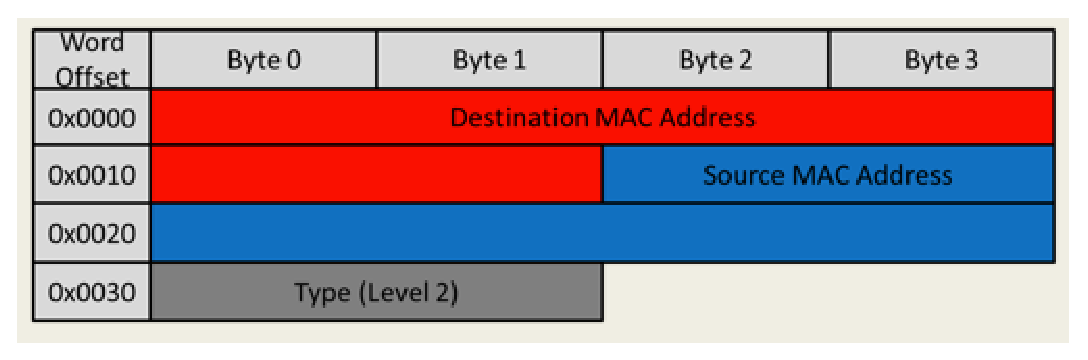
\includegraphics[scale=0.75]{eps/level1Header.eps}
\caption{The Level 1 Ethernet Header\cite{37}}
\label{level1Header}
\end{figure}
 
\vspace{1mm}
\noindent
{\bf The Destination MAC address}
\begin{verbatim}
0000 -- 0xd4, 0xbe, 0xd9, 0x50, 0xfa, 0xb2,             /* ...P..@< */
\end{verbatim}
That is, D4:BE:D9:50:FA:B2

\vspace{1mm}
\noindent
{\bf The Source MAC address}
\begin{verbatim}
0000 --                                     0x40, 0x3c, /* ...P..@< */
0008 -- 0xfc, 0x01, 0x04, 0x85,                         /* ......E. */
\end{verbatim}
That is, 40:3C:FC:01:04:85

\vspace{1mm}
\noindent
{\bf Type} 
\begin{verbatim}
0008 --                         0x08, 0x00,             /* ......E. */
\end{verbatim}
If the type field of the Ethernet header contains 0x0800 (which
this does) there will be a second nested level. The contents of
this level are described by the IP header. 

\begin{figure}[ht!]
\centering
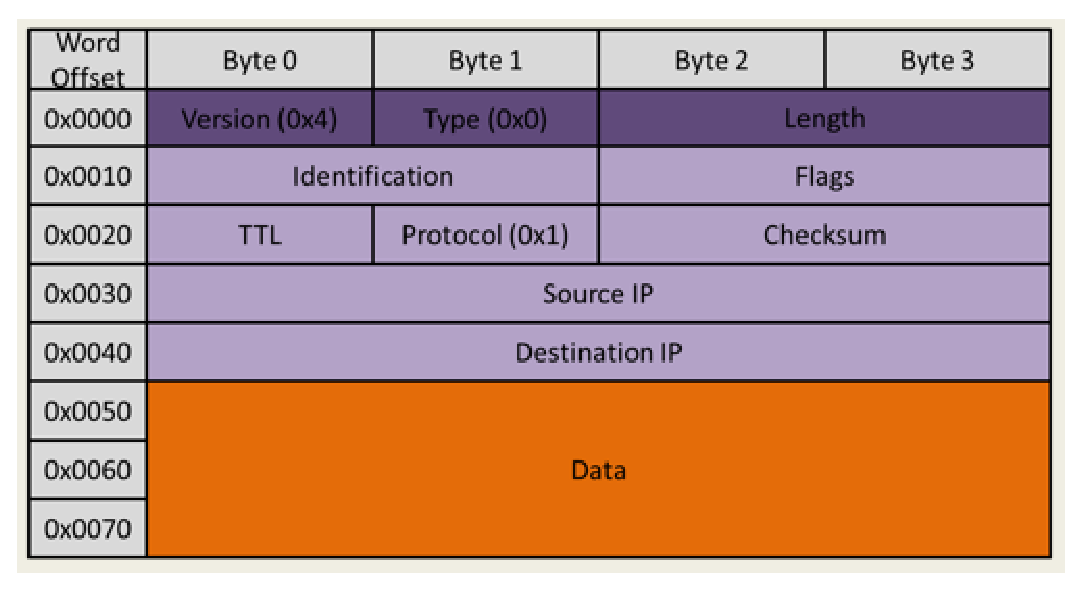
\includegraphics[scale=0.75]{eps/level2Header.eps}
\caption{The Level 2 IP Ethernet Header\cite{37}}
\label{level2Header}
\end{figure}

\vspace{1mm}
\noindent
{\bf Version} (4 bits)
\begin{verbatim}
0008 --                                     0x4 ,       /* ......E. */
\end{verbatim}
The Version is 4, which signals IPv4

\vspace{1mm}
\noindent
{\bf Internet Header Length} (4 bits)
\begin{verbatim}
0008 --                                       0x 5,     /* ......E. */
\end{verbatim}
The Internet Header Length is 5, which means 5x32 = 160 bits =20 bytes

\vspace{1mm}
\noindent
{\bf Type of Service} (1 byte)
\begin{verbatim}
0008 --                                           0x08, /* ......E. */
\end{verbatim}
This field is actually 2 fields, a 6-bit Differentiated Servies Code Point
and and Explicit Congestion Notification (2 bit). \cite{41}

\vspace{1mm}
\noindent
{\bf Total Length} (2 bytes)
\begin{verbatim}
0010 -- 0x05, 0xdc,                                     /* ..rD@.@. */
\end{verbatim}
Hex 0x5DC = 1500

\vspace{1mm}
\noindent
{\bf Identification} (2 bytes)
\begin{verbatim}
0010 --             0x72, 0x44,                         /* ..rD@.@. */
\end{verbatim}
The identiication field is primarily used for uniquely identifying the
group of fragments of a single IP datagram. \cite{41}

\vspace{1mm}
\noindent
{\bf Flags} (3 bits)
\begin{verbatim}
0010 --                         0x4                     /* ..rD@.@. */
0010 --                         0x 0, 0x00              /* ..rD@.@. */
\end{verbatim}
This 3-bit field is used to control or identify fragments.
This has the Don't Fragment (DF) bit set.\cite{41}

\vspace{1mm}
\noindent
{\bf Fragmentation Offset} (13 bits)
\begin{verbatim}
0010 --                         0x 0, 0x00              /* ..rD@.@. */
\end{verbatim}
The packet is not fragmented so there is no offset.

\vspace{1mm}
\noindent
{\bf Time to Live} (1 byte)
\begin{verbatim}
0010 --                                     0x40        /* ..rD@.@. */
\end{verbatim}
Supposed to be a number of seconds but is usually a hop count.

\vspace{1mm}
\noindent
{\bf Protocol} (1 bytes) \cite{43}
\begin{verbatim}
0010 --                                           0x06, /* ..rD@.@. */
\end{verbatim}
The 6 identifies this as a TCP packet. Note the FTP is a TCP-based
protocol.

\vspace{1mm}
\noindent
{\bf Header Checksum} (2 bytes)
\begin{verbatim}
0018 -- 0x3f, 0x7c, 0xc0, 0xa8                          /* ?|...... */
\end{verbatim}
0x3F7CC0A8 = 1065140392

\vspace{1mm}
\noindent
RFC 1071 defines the checksum calculation:

The checksum field is the 16-bit one's complement of the one's
complement sum of all 16-bit words in the header. For purposes of
computing the checksum, the value of the checksum field is zero.

\vspace{1mm}
\noindent
For example, consider 
\begin{verbatim} 
Hex 4500003044224000800600008c7c19acae241e2b
\end{verbatim}
(20 bytes IP header), using a machine which uses standard two's 
complement arithmetic:
\begin{enumerate}
\item 4500 + 0030 + 4422 + 4000 + 8006 + 0000 + 8c7c + 19ac + ae24 + 1e2b =
 0002BBCF (32-bit sum)
\item 0002 + BBCF = BBD1 = 1011101111010001 (1's complement 16-bit sum, 
formed by ``end around carry'' of 32-bit 2's complement sum)
\item ~BBD1 = 0100010000101110 = 442E (1's complement of 1's complement 
16-bit sum)
\end{enumerate}
To validate a header's checksum the same algorithm may be used - the 
checksum of a header which contains a correct checksum field is a word 
containing all zeros (value 0):
\begin{verbatim}
2BBCF + 442E = 2FFFD. 2 + FFFD = FFFF. the 1's complement of FFFF = 0.
\end{verbatim}

\vspace{1mm}
\noindent
{\bf The Source Address} (4 bytes)
\begin{verbatim}
0018 --                         0x01, 0x02, 0xc0, 0xa8, /* ?|...... */
\end{verbatim}
This is 192.168.1.2

\vspace{1mm}
\noindent
{\bf The Destination Address} (4 bytes)
\begin{verbatim}
0020 -- 0x01, 0x01, 0x00, 0x14,                         /* .....u.. */
\end{verbatim}
This appears to be 0.20.1.1 (which is nonsense)

\vspace{1mm}
\noindent
These bytes still need to be explained:
\begin{verbatim}
0020 --                         0xdf, 0x75, 0xe1, 0x89, /* .....u.. */
0028 -- 0xc7, 0x42, 0x28, 0x0a, 0x7e, 0xea, 0x80, 0x10, /* .B(.~... */
0030 -- 0x01, 0xc9, 0x8b, 0x61, 0x00, 0x00, 0x01, 0x01, /* ...a.... */
\end{verbatim}

\vspace{1mm}
\noindent
The {\bf Data} packet (offset x42)
\begin{verbatim}
  i     m     p     o     r     t
0042 -- 0x69, 0x6d, 0x70, 0x6f, 0x72, 0x74, /* import */
\end{verbatim}
The data packet length is 1514-66=1448 bytes (x42=66, the header length).

\begin{chunk}{referenceFrames}
/* Frame (1514 bytes) */
static const unsigned char pkt11[1514] = {
0xd4, 0xbe, 0xd9, 0x50, 0xfa, 0xb2, 0x40, 0x3c, /* ...P..@< */
0xfc, 0x01, 0x04, 0x85, 0x08, 0x00, 0x45, 0x08, /* ......E. */
0x05, 0xdc, 0x72, 0x44, 0x40, 0x00, 0x40, 0x06, /* ..rD@.@. */
0x3f, 0x7c, 0xc0, 0xa8, 0x01, 0x02, 0xc0, 0xa8, /* ?|...... */
0x01, 0x01, 0x00, 0x14, 0xdf, 0x75, 0xe1, 0x89, /* .....u.. */
0xc7, 0x42, 0x28, 0x0a, 0x7e, 0xea, 0x80, 0x10, /* .B(.~... */
0x01, 0xc9, 0x8b, 0x61, 0x00, 0x00, 0x01, 0x01, /* ...a.... */
0x08, 0x0a, 0x00, 0xf8, 0xb5, 0x03, 0x00, 0x07, /* ........ */
0x27, 0x99, 0x69, 0x6d, 0x70, 0x6f, 0x72, 0x74, /* '.import */
0x20, 0x6a, 0x61, 0x76, 0x61, 0x2e, 0x69, 0x6f, /*  java.io */
0x2e, 0x49, 0x4f, 0x45, 0x78, 0x63, 0x65, 0x70, /* .IOExcep */
0x74, 0x69, 0x6f, 0x6e, 0x3b, 0x0a, 0x69, 0x6d, /* tion;.im */
0x70, 0x6f, 0x72, 0x74, 0x20, 0x6a, 0x61, 0x76, /* port jav */
0x61, 0x2e, 0x75, 0x74, 0x69, 0x6c, 0x2e, 0x41, /* a.util.A */
0x72, 0x72, 0x61, 0x79, 0x4c, 0x69, 0x73, 0x74, /* rrayList */
0x3b, 0x0a, 0x69, 0x6d, 0x70, 0x6f, 0x72, 0x74, /* ;.import */
0x20, 0x6a, 0x61, 0x76, 0x61, 0x2e, 0x75, 0x74, /*  java.ut */
0x69, 0x6c, 0x2e, 0x43, 0x6f, 0x6c, 0x6c, 0x65, /* il.Colle */
0x63, 0x74, 0x69, 0x6f, 0x6e, 0x3b, 0x0a, 0x69, /* ction;.i */
0x6d, 0x70, 0x6f, 0x72, 0x74, 0x20, 0x6a, 0x61, /* mport ja */
0x76, 0x61, 0x2e, 0x75, 0x74, 0x69, 0x6c, 0x2e, /* va.util. */
0x4c, 0x69, 0x73, 0x74, 0x3b, 0x0a, 0x69, 0x6d, /* List;.im */
0x70, 0x6f, 0x72, 0x74, 0x20, 0x6f, 0x72, 0x67, /* port org */
0x2e, 0x61, 0x70, 0x61, 0x63, 0x68, 0x65, 0x2e, /* .apache. */
0x63, 0x6f, 0x6d, 0x6d, 0x6f, 0x6e, 0x73, 0x2e, /* commons. */
0x63, 0x6f, 0x6e, 0x66, 0x69, 0x67, 0x75, 0x72, /* configur */
0x61, 0x74, 0x69, 0x6f, 0x6e, 0x2e, 0x43, 0x6f, /* ation.Co */
0x6e, 0x66, 0x69, 0x67, 0x75, 0x72, 0x61, 0x74, /* nfigurat */
0x69, 0x6f, 0x6e, 0x45, 0x78, 0x63, 0x65, 0x70, /* ionExcep */
0x74, 0x69, 0x6f, 0x6e, 0x3b, 0x0a, 0x69, 0x6d, /* tion;.im */
0x70, 0x6f, 0x72, 0x74, 0x20, 0x6f, 0x72, 0x67, /* port org */
0x2e, 0x61, 0x70, 0x61, 0x63, 0x68, 0x65, 0x2e, /* .apache. */
0x75, 0x69, 0x6d, 0x61, 0x2e, 0x55, 0x69, 0x6d, /* uima.Uim */
0x61, 0x43, 0x6f, 0x6e, 0x74, 0x65, 0x78, 0x74, /* aContext */
0x3b, 0x0a, 0x69, 0x6d, 0x70, 0x6f, 0x72, 0x74, /* ;.import */
0x20, 0x6f, 0x72, 0x67, 0x2e, 0x61, 0x70, 0x61, /*  org.apa */
0x63, 0x68, 0x65, 0x2e, 0x75, 0x69, 0x6d, 0x61, /* che.uima */
0x2e, 0x61, 0x6e, 0x61, 0x6c, 0x79, 0x73, 0x69, /* .analysi */
0x73, 0x5f, 0x63, 0x6f, 0x6d, 0x70, 0x6f, 0x6e, /* s_compon */
0x65, 0x6e, 0x74, 0x2e, 0x4a, 0x43, 0x61, 0x73, /* ent.JCas */
0x41, 0x6e, 0x6e, 0x6f, 0x74, 0x61, 0x74, 0x6f, /* Annotato */
0x72, 0x5f, 0x49, 0x6d, 0x70, 0x6c, 0x42, 0x61, /* r_ImplBa */
0x73, 0x65, 0x3b, 0x0a, 0x69, 0x6d, 0x70, 0x6f, /* se;.impo */
0x72, 0x74, 0x20, 0x6f, 0x72, 0x67, 0x2e, 0x61, /* rt org.a */
0x70, 0x61, 0x63, 0x68, 0x65, 0x2e, 0x75, 0x69, /* pache.ui */
0x6d, 0x61, 0x2e, 0x61, 0x6e, 0x61, 0x6c, 0x79, /* ma.analy */
0x73, 0x69, 0x73, 0x5f, 0x65, 0x6e, 0x67, 0x69, /* sis_engi */
0x6e, 0x65, 0x2e, 0x41, 0x6e, 0x61, 0x6c, 0x79, /* ne.Analy */
0x73, 0x69, 0x73, 0x45, 0x6e, 0x67, 0x69, 0x6e, /* sisEngin */
0x65, 0x50, 0x72, 0x6f, 0x63, 0x65, 0x73, 0x73, /* eProcess */
0x45, 0x78, 0x63, 0x65, 0x70, 0x74, 0x69, 0x6f, /* Exceptio */
0x6e, 0x3b, 0x0a, 0x69, 0x6d, 0x70, 0x6f, 0x72, /* n;.impor */
0x74, 0x20, 0x6f, 0x72, 0x67, 0x2e, 0x61, 0x70, /* t org.ap */
0x61, 0x63, 0x68, 0x65, 0x2e, 0x75, 0x69, 0x6d, /* ache.uim */
0x61, 0x2e, 0x63, 0x61, 0x73, 0x2e, 0x46, 0x53, /* a.cas.FS */
0x49, 0x74, 0x65, 0x72, 0x61, 0x74, 0x6f, 0x72, /* Iterator */
0x3b, 0x0a, 0x69, 0x6d, 0x70, 0x6f, 0x72, 0x74, /* ;.import */
0x20, 0x6f, 0x72, 0x67, 0x2e, 0x61, 0x70, 0x61, /*  org.apa */
0x63, 0x68, 0x65, 0x2e, 0x75, 0x69, 0x6d, 0x61, /* che.uima */
0x2e, 0x6a, 0x63, 0x61, 0x73, 0x2e, 0x4a, 0x43, /* .jcas.JC */
0x61, 0x73, 0x3b, 0x0a, 0x69, 0x6d, 0x70, 0x6f, /* as;.impo */
0x72, 0x74, 0x20, 0x6f, 0x72, 0x67, 0x2e, 0x61, /* rt org.a */
0x70, 0x61, 0x63, 0x68, 0x65, 0x2e, 0x75, 0x69, /* pache.ui */
0x6d, 0x61, 0x2e, 0x6a, 0x63, 0x61, 0x73, 0x2e, /* ma.jcas. */
0x63, 0x61, 0x73, 0x2e, 0x46, 0x53, 0x4c, 0x69, /* cas.FSLi */
0x73, 0x74, 0x3b, 0x0a, 0x69, 0x6d, 0x70, 0x6f, /* st;.impo */
0x72, 0x74, 0x20, 0x6f, 0x72, 0x67, 0x2e, 0x61, /* rt org.a */
0x70, 0x61, 0x63, 0x68, 0x65, 0x2e, 0x75, 0x69, /* pache.ui */
0x6d, 0x61, 0x2e, 0x6a, 0x63, 0x61, 0x73, 0x2e, /* ma.jcas. */
0x63, 0x61, 0x73, 0x2e, 0x53, 0x74, 0x72, 0x69, /* cas.Stri */
0x6e, 0x67, 0x4c, 0x69, 0x73, 0x74, 0x3b, 0x0a, /* ngList;. */
0x69, 0x6d, 0x70, 0x6f, 0x72, 0x74, 0x20, 0x6f, /* import o */
0x72, 0x67, 0x2e, 0x61, 0x70, 0x61, 0x63, 0x68, /* rg.apach */
0x65, 0x2e, 0x75, 0x69, 0x6d, 0x61, 0x2e, 0x72, /* e.uima.r */
0x65, 0x73, 0x6f, 0x75, 0x72, 0x63, 0x65, 0x2e, /* esource. */
0x52, 0x65, 0x73, 0x6f, 0x75, 0x72, 0x63, 0x65, /* Resource */
0x49, 0x6e, 0x69, 0x74, 0x69, 0x61, 0x6c, 0x69, /* Initiali */
0x7a, 0x61, 0x74, 0x69, 0x6f, 0x6e, 0x45, 0x78, /* zationEx */
0x63, 0x65, 0x70, 0x74, 0x69, 0x6f, 0x6e, 0x3b, /* ception; */
0x0a, 0x69, 0x6d, 0x70, 0x6f, 0x72, 0x74, 0x20, /* .import  */
0x75, 0x74, 0x69, 0x6c, 0x2e, 0x2a, 0x3b, 0x0a, /* util.*;. */
0x69, 0x6d, 0x70, 0x6f, 0x72, 0x74, 0x20, 0x65, /* import e */
0x64, 0x75, 0x2e, 0x63, 0x6d, 0x75, 0x2e, 0x6c, /* du.cmu.l */
0x74, 0x69, 0x2e, 0x6f, 0x61, 0x71, 0x61, 0x2e, /* ti.oaqa. */
0x62, 0x69, 0x6f, 0x2e, 0x62, 0x69, 0x6f, 0x61, /* bio.bioa */
0x73, 0x71, 0x2e, 0x73, 0x65, 0x72, 0x76, 0x69, /* sq.servi */
0x63, 0x65, 0x73, 0x2e, 0x47, 0x6f, 0x50, 0x75, /* ces.GoPu */
0x62, 0x4d, 0x65, 0x64, 0x53, 0x65, 0x72, 0x76, /* bMedServ */
0x69, 0x63, 0x65, 0x3b, 0x0a, 0x69, 0x6d, 0x70, /* ice;.imp */
0x6f, 0x72, 0x74, 0x20, 0x65, 0x64, 0x75, 0x2e, /* ort edu. */
0x63, 0x6d, 0x75, 0x2e, 0x6c, 0x74, 0x69, 0x2e, /* cmu.lti. */
0x6f, 0x61, 0x71, 0x61, 0x2e, 0x62, 0x69, 0x6f, /* oaqa.bio */
0x2e, 0x62, 0x69, 0x6f, 0x61, 0x73, 0x71, 0x2e, /* .bioasq. */
0x73, 0x65, 0x72, 0x76, 0x69, 0x63, 0x65, 0x73, /* services */
0x2e, 0x4c, 0x69, 0x6e, 0x6b, 0x65, 0x64, 0x4c, /* .LinkedL */
0x69, 0x66, 0x65, 0x44, 0x61, 0x74, 0x61, 0x53, /* ifeDataS */
0x65, 0x72, 0x76, 0x69, 0x63, 0x65, 0x52, 0x65, /* erviceRe */
0x73, 0x70, 0x6f, 0x6e, 0x73, 0x65, 0x3b, 0x0a, /* sponse;. */
0x69, 0x6d, 0x70, 0x6f, 0x72, 0x74, 0x20, 0x65, /* import e */
0x64, 0x75, 0x2e, 0x63, 0x6d, 0x75, 0x2e, 0x6c, /* du.cmu.l */
0x74, 0x69, 0x2e, 0x6f, 0x61, 0x71, 0x61, 0x2e, /* ti.oaqa. */
0x62, 0x69, 0x6f, 0x2e, 0x62, 0x69, 0x6f, 0x61, /* bio.bioa */
0x73, 0x71, 0x2e, 0x73, 0x65, 0x72, 0x76, 0x69, /* sq.servi */
0x63, 0x65, 0x73, 0x2e, 0x4f, 0x6e, 0x74, 0x6f, /* ces.Onto */
0x6c, 0x6f, 0x67, 0x79, 0x53, 0x65, 0x72, 0x76, /* logyServ */
0x69, 0x63, 0x65, 0x52, 0x65, 0x73, 0x70, 0x6f, /* iceRespo */
0x6e, 0x73, 0x65, 0x3b, 0x0a, 0x69, 0x6d, 0x70, /* nse;.imp */
0x6f, 0x72, 0x74, 0x20, 0x65, 0x64, 0x75, 0x2e, /* ort edu. */
0x63, 0x6d, 0x75, 0x2e, 0x6c, 0x74, 0x69, 0x2e, /* cmu.lti. */
0x6f, 0x61, 0x71, 0x61, 0x2e, 0x62, 0x69, 0x6f, /* oaqa.bio */
0x2e, 0x62, 0x69, 0x6f, 0x61, 0x73, 0x71, 0x2e, /* .bioasq. */
0x73, 0x65, 0x72, 0x76, 0x69, 0x63, 0x65, 0x73, /* services */
0x2e, 0x50, 0x75, 0x62, 0x4d, 0x65, 0x64, 0x53, /* .PubMedS */
0x65, 0x61, 0x72, 0x63, 0x68, 0x53, 0x65, 0x72, /* earchSer */
0x76, 0x69, 0x63, 0x65, 0x52, 0x65, 0x73, 0x70, /* viceResp */
0x6f, 0x6e, 0x73, 0x65, 0x3b, 0x0a, 0x69, 0x6d, /* onse;.im */
0x70, 0x6f, 0x72, 0x74, 0x20, 0x65, 0x64, 0x75, /* port edu */
0x2e, 0x63, 0x6d, 0x75, 0x2e, 0x6c, 0x74, 0x69, /* .cmu.lti */
0x2e, 0x6f, 0x61, 0x71, 0x61, 0x2e, 0x62, 0x69, /* .oaqa.bi */
0x6f, 0x2e, 0x62, 0x69, 0x6f, 0x61, 0x73, 0x71, /* o.bioasq */
0x2e, 0x73, 0x65, 0x72, 0x76, 0x69, 0x63, 0x65, /* .service */
0x73, 0x2e, 0x50, 0x75, 0x62, 0x4d, 0x65, 0x64, /* s.PubMed */
0x53, 0x65, 0x61, 0x72, 0x63, 0x68, 0x53, 0x65, /* SearchSe */
0x72, 0x76, 0x69, 0x63, 0x65, 0x52, 0x65, 0x73, /* rviceRes */
0x70, 0x6f, 0x6e, 0x73, 0x65, 0x2e, 0x44, 0x6f, /* ponse.Do */
0x63, 0x75, 0x6d, 0x65, 0x6e, 0x74, 0x3b, 0x0a, /* cument;. */
0x69, 0x6d, 0x70, 0x6f, 0x72, 0x74, 0x20, 0x65, /* import e */
0x64, 0x75, 0x2e, 0x63, 0x6d, 0x75, 0x2e, 0x6c, /* du.cmu.l */
0x74, 0x69, 0x2e, 0x6f, 0x61, 0x71, 0x61, 0x2e, /* ti.oaqa. */
0x74, 0x79, 0x70, 0x65, 0x2e, 0x69, 0x6e, 0x70, /* type.inp */
0x75, 0x74, 0x2e, 0x51, 0x75, 0x65, 0x73, 0x74, /* ut.Quest */
0x69, 0x6f, 0x6e, 0x3b, 0x0a, 0x69, 0x6d, 0x70, /* ion;.imp */
0x6f, 0x72, 0x74, 0x20, 0x65, 0x64, 0x75, 0x2e, /* ort edu. */
0x63, 0x6d, 0x75, 0x2e, 0x6c, 0x74, 0x69, 0x2e, /* cmu.lti. */
0x6f, 0x61, 0x71, 0x61, 0x2e, 0x74, 0x79, 0x70, /* oaqa.typ */
0x65, 0x2e, 0x6b, 0x62, 0x2e, 0x43, 0x6f, 0x6e, /* e.kb.Con */
0x63, 0x65, 0x70, 0x74, 0x3b, 0x0a, 0x69, 0x6d, /* cept;.im */
0x70, 0x6f, 0x72, 0x74, 0x20, 0x65, 0x64, 0x75, /* port edu */
0x2e, 0x63, 0x6d, 0x75, 0x2e, 0x6c, 0x74, 0x69, /* .cmu.lti */
0x2e, 0x6f, 0x61, 0x71, 0x61, 0x2e, 0x74, 0x79, /* .oaqa.ty */
0x70, 0x65, 0x2e, 0x6b, 0x62, 0x2e, 0x54, 0x72, /* pe.kb.Tr */
0x69, 0x70, 0x6c, 0x65, 0x3b, 0x0a, 0x0a, 0x70, /* iple;..p */
0x75, 0x62, 0x6c, 0x69, 0x63, 0x20, 0x63, 0x6c, /* ublic cl */
0x61, 0x73, 0x73, 0x20, 0x41, 0x6e, 0x6e, 0x6f, /* ass Anno */
0x74, 0x61, 0x74, 0x6f, 0x72, 0x20, 0x65, 0x78, /* tator ex */
0x74, 0x65, 0x6e, 0x64, 0x73, 0x20, 0x4a, 0x43, /* tends JC */
0x61, 0x73, 0x41, 0x6e, 0x6e, 0x6f, 0x74, 0x61, /* asAnnota */
0x74, 0x6f, 0x72, 0x5f, 0x49, 0x6d, 0x70, 0x6c, /* tor_Impl */
0x42, 0x61, 0x73, 0x65, 0x20, 0x7b, 0x0a, 0x20, /* Base {.  */
0x20, 0x73, 0x74, 0x61, 0x74, 0x69, 0x63, 0x20, /*  static  */
0x47, 0x6f, 0x50, 0x75, 0x62, 0x4d, 0x65, 0x64, /* GoPubMed */
0x53, 0x65, 0x72, 0x76, 0x69, 0x63, 0x65, 0x20, /* Service  */
0x73, 0x65, 0x72, 0x76, 0x69, 0x63, 0x65, 0x20, /* service  */
0x3d, 0x20, 0x6e, 0x75, 0x6c, 0x6c, 0x3b, 0x0a, /* = null;. */
0x0a, 0x20, 0x20, 0x40, 0x4f, 0x76, 0x65, 0x72, /* .  @Over */
0x72, 0x69, 0x64, 0x65, 0x0a, 0x20, 0x20, 0x70, /* ride.  p */
0x75, 0x62, 0x6c, 0x69, 0x63, 0x20, 0x76, 0x6f, /* ublic vo */
0x69, 0x64, 0x20, 0x69, 0x6e, 0x69, 0x74, 0x69, /* id initi */
0x61, 0x6c, 0x69, 0x7a, 0x65, 0x28, 0x55, 0x69, /* alize(Ui */
0x6d, 0x61, 0x43, 0x6f, 0x6e, 0x74, 0x65, 0x78, /* maContex */
0x74, 0x20, 0x61, 0x43, 0x6f, 0x6e, 0x74, 0x65, /* t aConte */
0x78, 0x74, 0x29, 0x20, 0x74, 0x68, 0x72, 0x6f, /* xt) thro */
0x77, 0x73, 0x20, 0x52, 0x65, 0x73, 0x6f, 0x75, /* ws Resou */
0x72, 0x63, 0x65, 0x49, 0x6e, 0x69, 0x74, 0x69, /* rceIniti */
0x61, 0x6c, 0x69, 0x7a, 0x61, 0x74, 0x69, 0x6f, /* alizatio */
0x6e, 0x45, 0x78, 0x63, 0x65, 0x70, 0x74, 0x69, /* nExcepti */
0x6f, 0x6e, 0x20, 0x7b, 0x0a, 0x20, 0x20, 0x20, /* on {.    */
0x20, 0x74, 0x72, 0x79, 0x20, 0x7b, 0x0a, 0x20, /*  try {.  */
0x20, 0x20, 0x20, 0x20, 0x20, 0x47, 0x6f, 0x50, /*      GoP */
0x75, 0x62, 0x4d, 0x65, 0x64, 0x53, 0x65, 0x72, /* ubMedSer */
0x76, 0x69, 0x63, 0x65, 0x20, 0x73, 0x65, 0x72, /* vice ser */
0x76, 0x69, 0x63, 0x65, 0x20, 0x3d, 0x20, 0x6e, /* vice = n */
0x65, 0x77, 0x20, 0x47, 0x6f, 0x50, 0x75, 0x62, /* ew GoPub */
0x4d, 0x65, 0x64, 0x53, 0x65, 0x72, 0x76, 0x69, /* MedServi */
0x63, 0x65, 0x28, 0x22, 0x2e, 0x2f, 0x70, 0x72, /* ce("./pr */
0x6f, 0x6a, 0x65, 0x63, 0x74, 0x2e, 0x70, 0x72, /* oject.pr */
0x6f, 0x70, 0x65, 0x72, 0x74, 0x69, 0x65, 0x73, /* operties */
0x22, 0x29, 0x3b, 0x0a, 0x20, 0x20, 0x20, 0x20, /* ");.     */
0x7d, 0x20, 0x63, 0x61, 0x74, 0x63, 0x68, 0x20, /* } catch  */
0x28, 0x43, 0x6f, 0x6e, 0x66, 0x69, 0x67, 0x75, /* (Configu */
0x72, 0x61, 0x74, 0x69, 0x6f, 0x6e, 0x45, 0x78, /* rationEx */
0x63, 0x65, 0x70, 0x74, 0x69, 0x6f, 0x6e, 0x20, /* ception  */
0x65, 0x29, 0x20, 0x7b, 0x0a, 0x20, 0x20, 0x20, /* e) {.    */
0x20, 0x20, 0x20, 0x2f, 0x2f, 0x20, 0x54, 0x4f, /*    // TO */
0x44, 0x4f, 0x20, 0x41, 0x75, 0x74, 0x6f, 0x2d, /* DO Auto- */
0x67, 0x65, 0x6e, 0x65, 0x72, 0x61, 0x74, 0x65, /* generate */
0x64, 0x20, 0x63, 0x61, 0x74, 0x63, 0x68, 0x20, /* d catch  */
0x62, 0x6c, 0x6f, 0x63, 0x6b, 0x0a, 0x20, 0x20, /* block.   */
0x20, 0x20, 0x20, 0x20, 0x65, 0x2e, 0x70, 0x72, /*     e.pr */
0x69, 0x6e                                      /* in */
};

/* Frame (1514 bytes) */
static const unsigned char pkt13[1514] = {
0xd4, 0xbe, 0xd9, 0x50, 0xfa, 0xb2, 0x40, 0x3c, /* ...P..@< */
0xfc, 0x01, 0x04, 0x85, 0x08, 0x00, 0x45, 0x08, /* ......E. */
0x05, 0xdc, 0x72, 0x45, 0x40, 0x00, 0x40, 0x06, /* ..rE@.@. */
0x3f, 0x7b, 0xc0, 0xa8, 0x01, 0x02, 0xc0, 0xa8, /* ?{...... */
0x01, 0x01, 0x00, 0x14, 0xdf, 0x75, 0xe1, 0x89, /* .....u.. */
0xcc, 0xea, 0x28, 0x0a, 0x7e, 0xea, 0x80, 0x10, /* ..(.~... */
0x01, 0xc9, 0x0a, 0x8a, 0x00, 0x00, 0x01, 0x01, /* ........ */
0x08, 0x0a, 0x00, 0xf8, 0xb5, 0x03, 0x00, 0x07, /* ........ */
0x27, 0x99, 0x74, 0x53, 0x74, 0x61, 0x63, 0x6b, /* '.tStack */
0x54, 0x72, 0x61, 0x63, 0x65, 0x28, 0x29, 0x3b, /* Trace(); */
0x0a, 0x20, 0x20, 0x20, 0x20, 0x7d, 0x0a, 0x20, /* .    }.  */
0x20, 0x7d, 0x0a, 0x0a, 0x20, 0x20, 0x40, 0x4f, /*  }..  @O */
0x76, 0x65, 0x72, 0x72, 0x69, 0x64, 0x65, 0x0a, /* verride. */
0x20, 0x20, 0x70, 0x75, 0x62, 0x6c, 0x69, 0x63, /*   public */
0x20, 0x76, 0x6f, 0x69, 0x64, 0x20, 0x70, 0x72, /*  void pr */
0x6f, 0x63, 0x65, 0x73, 0x73, 0x28, 0x4a, 0x43, /* ocess(JC */
0x61, 0x73, 0x20, 0x61, 0x4a, 0x43, 0x61, 0x73, /* as aJCas */
0x29, 0x20, 0x74, 0x68, 0x72, 0x6f, 0x77, 0x73, /* ) throws */
0x20, 0x41, 0x6e, 0x61, 0x6c, 0x79, 0x73, 0x69, /*  Analysi */
0x73, 0x45, 0x6e, 0x67, 0x69, 0x6e, 0x65, 0x50, /* sEngineP */
0x72, 0x6f, 0x63, 0x65, 0x73, 0x73, 0x45, 0x78, /* rocessEx */
0x63, 0x65, 0x70, 0x74, 0x69, 0x6f, 0x6e, 0x20, /* ception  */
0x7b, 0x0a, 0x20, 0x20, 0x20, 0x20, 0x2f, 0x2f, /* {.    // */
0x20, 0x54, 0x4f, 0x44, 0x4f, 0x20, 0x41, 0x75, /*  TODO Au */
0x74, 0x6f, 0x2d, 0x67, 0x65, 0x6e, 0x65, 0x72, /* to-gener */
0x61, 0x74, 0x65, 0x64, 0x20, 0x6d, 0x65, 0x74, /* ated met */
0x68, 0x6f, 0x64, 0x20, 0x73, 0x74, 0x75, 0x62, /* hod stub */
0x0a, 0x20, 0x20, 0x20, 0x20, 0x46, 0x53, 0x49, /* .    FSI */
0x74, 0x65, 0x72, 0x61, 0x74, 0x6f, 0x72, 0x20, /* terator  */
0x69, 0x74, 0x20, 0x3d, 0x20, 0x61, 0x4a, 0x43, /* it = aJC */
0x61, 0x73, 0x2e, 0x67, 0x65, 0x74, 0x41, 0x6e, /* as.getAn */
0x6e, 0x6f, 0x74, 0x61, 0x74, 0x69, 0x6f, 0x6e, /* notation */
0x49, 0x6e, 0x64, 0x65, 0x78, 0x28, 0x51, 0x75, /* Index(Qu */
0x65, 0x73, 0x74, 0x69, 0x6f, 0x6e, 0x2e, 0x74, /* estion.t */
0x79, 0x70, 0x65, 0x29, 0x2e, 0x69, 0x74, 0x65, /* ype).ite */
0x72, 0x61, 0x74, 0x6f, 0x72, 0x28, 0x29, 0x3b, /* rator(); */
0x0a, 0x20, 0x20, 0x20, 0x20, 0x2f, 0x2f, 0x20, /* .    //  */
0x53, 0x74, 0x72, 0x69, 0x6e, 0x67, 0x20, 0x44, /* String D */
0x6f, 0x63, 0x20, 0x3d, 0x20, 0x61, 0x4a, 0x43, /* oc = aJC */
0x61, 0x73, 0x2e, 0x67, 0x65, 0x74, 0x44, 0x6f, /* as.getDo */
0x63, 0x75, 0x6d, 0x65, 0x6e, 0x74, 0x54, 0x65, /* cumentTe */
0x78, 0x74, 0x28, 0x29, 0x3b, 0x0a, 0x20, 0x20, /* xt();.   */
0x20, 0x20, 0x51, 0x75, 0x65, 0x73, 0x74, 0x69, /*   Questi */
0x6f, 0x6e, 0x20, 0x71, 0x75, 0x65, 0x73, 0x74, /* on quest */
0x69, 0x6f, 0x6e, 0x54, 0x79, 0x70, 0x65, 0x53, /* ionTypeS */
0x79, 0x73, 0x20, 0x3d, 0x20, 0x6e, 0x75, 0x6c, /* ys = nul */
0x6c, 0x3b, 0x0a, 0x20, 0x20, 0x20, 0x20, 0x69, /* l;.    i */
0x66, 0x20, 0x28, 0x69, 0x74, 0x2e, 0x68, 0x61, /* f (it.ha */
0x73, 0x4e, 0x65, 0x78, 0x74, 0x28, 0x29, 0x29, /* sNext()) */
0x20, 0x7b, 0x0a, 0x20, 0x20, 0x20, 0x20, 0x20, /*  {.      */
0x20, 0x71, 0x75, 0x65, 0x73, 0x74, 0x69, 0x6f, /*  questio */
0x6e, 0x54, 0x79, 0x70, 0x65, 0x53, 0x79, 0x73, /* nTypeSys */
0x20, 0x3d, 0x20, 0x28, 0x51, 0x75, 0x65, 0x73, /*  = (Ques */
0x74, 0x69, 0x6f, 0x6e, 0x29, 0x20, 0x69, 0x74, /* tion) it */
0x2e, 0x6e, 0x65, 0x78, 0x74, 0x28, 0x29, 0x3b, /* .next(); */
0x0a, 0x20, 0x20, 0x20, 0x20, 0x7d, 0x0a, 0x20, /* .    }.  */
0x20, 0x20, 0x20, 0x53, 0x74, 0x72, 0x69, 0x6e, /*    Strin */
0x67, 0x20, 0x74, 0x65, 0x78, 0x74, 0x20, 0x3d, /* g text = */
0x20, 0x71, 0x75, 0x65, 0x73, 0x74, 0x69, 0x6f, /*  questio */
0x6e, 0x54, 0x79, 0x70, 0x65, 0x53, 0x79, 0x73, /* nTypeSys */
0x2e, 0x67, 0x65, 0x74, 0x54, 0x65, 0x78, 0x74, /* .getText */
0x28, 0x29, 0x3b, 0x0a, 0x20, 0x20, 0x20, 0x20, /* ();.     */
0x43, 0x6f, 0x6e, 0x63, 0x65, 0x70, 0x74, 0x20, /* Concept  */
0x63, 0x6f, 0x6e, 0x63, 0x65, 0x70, 0x74, 0x54, /* conceptT */
0x79, 0x70, 0x65, 0x53, 0x79, 0x73, 0x20, 0x3d, /* ypeSys = */
0x20, 0x6e, 0x75, 0x6c, 0x6c, 0x3b, 0x0a, 0x20, /*  null;.  */
0x20, 0x20, 0x20, 0x2f, 0x2f, 0x20, 0x53, 0x74, /*    // St */
0x72, 0x69, 0x6e, 0x67, 0x4c, 0x69, 0x73, 0x74, /* ringList */
0x20, 0x63, 0x6f, 0x6e, 0x63, 0x65, 0x70, 0x74, /*  concept */
0x53, 0x74, 0x72, 0x69, 0x6e, 0x67, 0x4c, 0x69, /* StringLi */
0x73, 0x74, 0x20, 0x3d, 0x20, 0x6e, 0x75, 0x6c, /* st = nul */
0x6c, 0x3b, 0x0a, 0x20, 0x20, 0x20, 0x20, 0x2f, /* l;.    / */
0x2f, 0x20, 0x46, 0x53, 0x4c, 0x69, 0x73, 0x74, /* / FSList */
0x20, 0x6d, 0x65, 0x6e, 0x74, 0x69, 0x6f, 0x6e, /*  mention */
0x4c, 0x69, 0x73, 0x74, 0x20, 0x3d, 0x20, 0x6e, /* List = n */
0x75, 0x6c, 0x6c, 0x3b, 0x0a, 0x20, 0x20, 0x20, /* ull;.    */
0x20, 0x4c, 0x69, 0x73, 0x74, 0x3c, 0x53, 0x74, /*  List<St */
0x72, 0x69, 0x6e, 0x67, 0x3e, 0x20, 0x63, 0x6f, /* ring> co */
0x6e, 0x63, 0x65, 0x70, 0x74, 0x4c, 0x69, 0x73, /* nceptLis */
0x74, 0x20, 0x3d, 0x20, 0x6e, 0x75, 0x6c, 0x6c, /* t = null */
0x3b, 0x0a, 0x20, 0x20, 0x20, 0x20, 0x4c, 0x69, /* ;.    Li */
0x73, 0x74, 0x3c, 0x44, 0x6f, 0x75, 0x62, 0x6c, /* st<Doubl */
0x65, 0x3e, 0x20, 0x63, 0x6f, 0x6e, 0x66, 0x69, /* e> confi */
0x64, 0x65, 0x6e, 0x63, 0x65, 0x4c, 0x69, 0x73, /* denceLis */
0x74, 0x20, 0x3d, 0x20, 0x6e, 0x75, 0x6c, 0x6c, /* t = null */
0x3b, 0x0a, 0x20, 0x20, 0x20, 0x20, 0x65, 0x64, /* ;.    ed */
0x75, 0x2e, 0x63, 0x6d, 0x75, 0x2e, 0x6c, 0x74, /* u.cmu.lt */
0x69, 0x2e, 0x6f, 0x61, 0x71, 0x61, 0x2e, 0x74, /* i.oaqa.t */
0x79, 0x70, 0x65, 0x2e, 0x72, 0x65, 0x74, 0x72, /* ype.retr */
0x69, 0x65, 0x76, 0x61, 0x6c, 0x2e, 0x44, 0x6f, /* ieval.Do */
0x63, 0x75, 0x6d, 0x65, 0x6e, 0x74, 0x20, 0x64, /* cument d */
0x6f, 0x63, 0x75, 0x6d, 0x65, 0x6e, 0x74, 0x54, /* ocumentT */
0x79, 0x70, 0x65, 0x53, 0x79, 0x73, 0x20, 0x3d, /* ypeSys = */
0x20, 0x6e, 0x75, 0x6c, 0x6c, 0x3b, 0x0a, 0x20, /*  null;.  */
0x20, 0x20, 0x20, 0x2f, 0x2f, 0x20, 0x53, 0x74, /*    // St */
0x72, 0x69, 0x6e, 0x67, 0x4c, 0x69, 0x73, 0x74, /* ringList */
0x20, 0x64, 0x6f, 0x63, 0x75, 0x6d, 0x65, 0x6e, /*  documen */
0x74, 0x53, 0x74, 0x72, 0x69, 0x6e, 0x67, 0x4c, /* tStringL */
0x69, 0x73, 0x74, 0x20, 0x3d, 0x20, 0x6e, 0x75, /* ist = nu */
0x6c, 0x6c, 0x3b, 0x0a, 0x20, 0x20, 0x20, 0x20, /* ll;.     */
0x54, 0x72, 0x69, 0x70, 0x6c, 0x65, 0x20, 0x74, /* Triple t */
0x72, 0x69, 0x70, 0x6c, 0x65, 0x54, 0x79, 0x70, /* ripleTyp */
0x65, 0x53, 0x79, 0x73, 0x20, 0x3d, 0x20, 0x6e, /* eSys = n */
0x75, 0x6c, 0x6c, 0x3b, 0x0a, 0x20, 0x20, 0x20, /* ull;.    */
0x20, 0x74, 0x72, 0x79, 0x20, 0x7b, 0x0a, 0x20, /*  try {.  */
0x20, 0x20, 0x20, 0x20, 0x20, 0x4f, 0x6e, 0x74, /*      Ont */
0x6f, 0x6c, 0x6f, 0x67, 0x79, 0x53, 0x65, 0x72, /* ologySer */
0x76, 0x69, 0x63, 0x65, 0x52, 0x65, 0x73, 0x70, /* viceResp */
0x6f, 0x6e, 0x73, 0x65, 0x2e, 0x52, 0x65, 0x73, /* onse.Res */
0x75, 0x6c, 0x74, 0x20, 0x64, 0x69, 0x73, 0x65, /* ult dise */
0x61, 0x73, 0x65, 0x4f, 0x6e, 0x74, 0x6f, 0x6c, /* aseOntol */
0x6f, 0x67, 0x79, 0x52, 0x65, 0x73, 0x75, 0x6c, /* ogyResul */
0x74, 0x20, 0x3d, 0x20, 0x73, 0x65, 0x72, 0x76, /* t = serv */
0x69, 0x63, 0x65, 0x0a, 0x20, 0x20, 0x20, 0x20, /* ice.     */
0x20, 0x20, 0x20, 0x20, 0x20, 0x20, 0x20, 0x20, /*          */
0x20, 0x20, 0x2e, 0x66, 0x69, 0x6e, 0x64, 0x44, /*   .findD */
0x69, 0x73, 0x65, 0x61, 0x73, 0x65, 0x4f, 0x6e, /* iseaseOn */
0x74, 0x6f, 0x6c, 0x6f, 0x67, 0x79, 0x45, 0x6e, /* tologyEn */
0x74, 0x69, 0x74, 0x69, 0x65, 0x73, 0x50, 0x61, /* titiesPa */
0x67, 0x65, 0x64, 0x28, 0x74, 0x65, 0x78, 0x74, /* ged(text */
0x2c, 0x20, 0x30, 0x29, 0x3b, 0x0a, 0x20, 0x20, /* , 0);.   */
0x20, 0x20, 0x20, 0x20, 0x63, 0x6f, 0x6e, 0x63, /*     conc */
0x65, 0x70, 0x74, 0x4c, 0x69, 0x73, 0x74, 0x20, /* eptList  */
0x3d, 0x20, 0x6e, 0x65, 0x77, 0x20, 0x41, 0x72, /* = new Ar */
0x72, 0x61, 0x79, 0x4c, 0x69, 0x73, 0x74, 0x3c, /* rayList< */
0x53, 0x74, 0x72, 0x69, 0x6e, 0x67, 0x3e, 0x28, /* String>( */
0x29, 0x3b, 0x0a, 0x20, 0x20, 0x20, 0x20, 0x20, /* );.      */
0x20, 0x63, 0x6f, 0x6e, 0x66, 0x69, 0x64, 0x65, /*  confide */
0x6e, 0x63, 0x65, 0x4c, 0x69, 0x73, 0x74, 0x20, /* nceList  */
0x3d, 0x20, 0x6e, 0x65, 0x77, 0x20, 0x41, 0x72, /* = new Ar */
0x72, 0x61, 0x79, 0x4c, 0x69, 0x73, 0x74, 0x3c, /* rayList< */
0x44, 0x6f, 0x75, 0x62, 0x6c, 0x65, 0x3e, 0x28, /* Double>( */
0x29, 0x3b, 0x0a, 0x20, 0x20, 0x20, 0x20, 0x20, /* );.      */
0x20, 0x63, 0x6f, 0x6e, 0x63, 0x65, 0x70, 0x74, /*  concept */
0x54, 0x79, 0x70, 0x65, 0x53, 0x79, 0x73, 0x20, /* TypeSys  */
0x3d, 0x20, 0x6e, 0x65, 0x77, 0x20, 0x43, 0x6f, /* = new Co */
0x6e, 0x63, 0x65, 0x70, 0x74, 0x28, 0x61, 0x4a, /* ncept(aJ */
0x43, 0x61, 0x73, 0x29, 0x3b, 0x0a, 0x20, 0x20, /* Cas);.   */
0x20, 0x20, 0x20, 0x20, 0x66, 0x6f, 0x72, 0x20, /*     for  */
0x28, 0x4f, 0x6e, 0x74, 0x6f, 0x6c, 0x6f, 0x67, /* (Ontolog */
0x79, 0x53, 0x65, 0x72, 0x76, 0x69, 0x63, 0x65, /* yService */
0x52, 0x65, 0x73, 0x70, 0x6f, 0x6e, 0x73, 0x65, /* Response */
0x2e, 0x46, 0x69, 0x6e, 0x64, 0x69, 0x6e, 0x67, /* .Finding */
0x20, 0x66, 0x69, 0x6e, 0x64, 0x69, 0x6e, 0x67, /*  finding */
0x20, 0x3a, 0x20, 0x64, 0x69, 0x73, 0x65, 0x61, /*  : disea */
0x73, 0x65, 0x4f, 0x6e, 0x74, 0x6f, 0x6c, 0x6f, /* seOntolo */
0x67, 0x79, 0x52, 0x65, 0x73, 0x75, 0x6c, 0x74, /* gyResult */
0x2e, 0x67, 0x65, 0x74, 0x46, 0x69, 0x6e, 0x64, /* .getFind */
0x69, 0x6e, 0x67, 0x73, 0x28, 0x29, 0x29, 0x20, /* ings())  */
0x7b, 0x0a, 0x20, 0x20, 0x20, 0x20, 0x20, 0x20, /* {.       */
0x20, 0x20, 0x63, 0x6f, 0x6e, 0x63, 0x65, 0x70, /*   concep */
0x74, 0x4c, 0x69, 0x73, 0x74, 0x2e, 0x61, 0x64, /* tList.ad */
0x64, 0x28, 0x66, 0x69, 0x6e, 0x64, 0x69, 0x6e, /* d(findin */
0x67, 0x2e, 0x67, 0x65, 0x74, 0x43, 0x6f, 0x6e, /* g.getCon */
0x63, 0x65, 0x70, 0x74, 0x28, 0x29, 0x2e, 0x67, /* cept().g */
0x65, 0x74, 0x55, 0x72, 0x69, 0x28, 0x29, 0x29, /* etUri()) */
0x3b, 0x0a, 0x20, 0x20, 0x20, 0x20, 0x20, 0x20, /* ;.       */
0x20, 0x20, 0x63, 0x6f, 0x6e, 0x66, 0x69, 0x64, /*   confid */
0x65, 0x6e, 0x63, 0x65, 0x4c, 0x69, 0x73, 0x74, /* enceList */
0x2e, 0x61, 0x64, 0x64, 0x28, 0x66, 0x69, 0x6e, /* .add(fin */
0x64, 0x69, 0x6e, 0x67, 0x2e, 0x67, 0x65, 0x74, /* ding.get */
0x53, 0x63, 0x6f, 0x72, 0x65, 0x28, 0x29, 0x29, /* Score()) */
0x3b, 0x0a, 0x20, 0x20, 0x20, 0x20, 0x20, 0x20, /* ;.       */
0x7d, 0x0a, 0x20, 0x20, 0x20, 0x20, 0x20, 0x20, /* }.       */
0x63, 0x6f, 0x6e, 0x63, 0x65, 0x70, 0x74, 0x54, /* conceptT */
0x79, 0x70, 0x65, 0x53, 0x79, 0x73, 0x2e, 0x73, /* ypeSys.s */
0x65, 0x74, 0x4e, 0x61, 0x6d, 0x65, 0x28, 0x22, /* etName(" */
0x44, 0x69, 0x73, 0x65, 0x61, 0x73, 0x65, 0x20, /* Disease  */
0x4f, 0x6e, 0x74, 0x6f, 0x6c, 0x6f, 0x67, 0x79, /* Ontology */
0x22, 0x29, 0x3b, 0x0a, 0x20, 0x20, 0x20, 0x20, /* ");.     */
0x20, 0x20, 0x2f, 0x2f, 0x63, 0x6f, 0x6e, 0x63, /*   //conc */
0x65, 0x70, 0x74, 0x54, 0x79, 0x70, 0x65, 0x53, /* eptTypeS */
0x79, 0x73, 0x2e, 0x73, 0x65, 0x74, 0x55, 0x72, /* ys.setUr */
0x69, 0x73, 0x28, 0x55, 0x74, 0x69, 0x6c, 0x73, /* is(Utils */
0x2e, 0x63, 0x72, 0x65, 0x61, 0x74, 0x65, 0x53, /* .createS */
0x74, 0x72, 0x69, 0x6e, 0x67, 0x4c, 0x69, 0x73, /* tringLis */
0x74, 0x28, 0x61, 0x4a, 0x43, 0x61, 0x73, 0x2c, /* t(aJCas, */
0x20, 0x63, 0x6f, 0x6e, 0x63, 0x65, 0x70, 0x74, /*  concept */
0x4c, 0x69, 0x73, 0x74, 0x29, 0x29, 0x3b, 0x0a, /* List));. */
0x20, 0x20, 0x20, 0x20, 0x20, 0x20, 0x2f, 0x2f, /*       // */
0x63, 0x6f, 0x6e, 0x63, 0x65, 0x70, 0x74, 0x54, /* conceptT */
0x79, 0x70, 0x65, 0x53, 0x79, 0x73, 0x2e, 0x73, /* ypeSys.s */
0x65, 0x74, 0x4d, 0x65, 0x6e, 0x74, 0x69, 0x6f, /* etMentio */
0x6e, 0x73, 0x28, 0x55, 0x74, 0x69, 0x6c, 0x73, /* ns(Utils */
0x2e, 0x66, 0x72, 0x6f, 0x6d, 0x43, 0x6f, 0x6c, /* .fromCol */
0x6c, 0x65, 0x63, 0x74, 0x69, 0x6f, 0x6e, 0x54, /* lectionT */
0x6f, 0x46, 0x53, 0x4c, 0x69, 0x73, 0x74, 0x28, /* oFSList( */
0x61, 0x4a, 0x43, 0x61, 0x73, 0x2c, 0x20, 0x28, /* aJCas, ( */
0x43, 0x6f, 0x6c, 0x6c, 0x65, 0x63, 0x74, 0x69, /* Collecti */
0x6f, 0x6e                                      /* on */
};

/* Frame (1266 bytes) */
static const unsigned char pkt15[1266] = {
0xd4, 0xbe, 0xd9, 0x50, 0xfa, 0xb2, 0x40, 0x3c, /* ...P..@< */
0xfc, 0x01, 0x04, 0x85, 0x08, 0x00, 0x45, 0x08, /* ......E. */
0x04, 0xe4, 0x72, 0x46, 0x40, 0x00, 0x40, 0x06, /* ..rF@.@. */
0x40, 0x72, 0xc0, 0xa8, 0x01, 0x02, 0xc0, 0xa8, /* @r...... */
0x01, 0x01, 0x00, 0x14, 0xdf, 0x75, 0xe1, 0x89, /* .....u.. */
0xd2, 0x92, 0x28, 0x0a, 0x7e, 0xea, 0x80, 0x18, /* ..(.~... */
0x01, 0xc9, 0xd6, 0xe6, 0x00, 0x00, 0x01, 0x01, /* ........ */
0x08, 0x0a, 0x00, 0xf8, 0xb5, 0x03, 0x00, 0x07, /* ........ */
0x27, 0x99, 0x29, 0x20, 0x63, 0x6f, 0x6e, 0x66, /* '.) conf */
0x69, 0x64, 0x65, 0x6e, 0x63, 0x65, 0x4c, 0x69, /* idenceLi */
0x73, 0x74, 0x29, 0x29, 0x3b, 0x0a, 0x20, 0x20, /* st));.   */
0x20, 0x20, 0x20, 0x20, 0x63, 0x6f, 0x6e, 0x63, /*     conc */
0x65, 0x70, 0x74, 0x54, 0x79, 0x70, 0x65, 0x53, /* eptTypeS */
0x79, 0x73, 0x2e, 0x61, 0x64, 0x64, 0x54, 0x6f, /* ys.addTo */
0x49, 0x6e, 0x64, 0x65, 0x78, 0x65, 0x73, 0x28, /* Indexes( */
0x61, 0x4a, 0x43, 0x61, 0x73, 0x29, 0x3b, 0x0a, /* aJCas);. */
0x20, 0x20, 0x20, 0x20, 0x20, 0x20, 0x63, 0x6f, /*       co */
0x6e, 0x63, 0x65, 0x70, 0x74, 0x4c, 0x69, 0x73, /* nceptLis */
0x74, 0x20, 0x3d, 0x20, 0x6e, 0x65, 0x77, 0x20, /* t = new  */
0x41, 0x72, 0x72, 0x61, 0x79, 0x4c, 0x69, 0x73, /* ArrayLis */
0x74, 0x3c, 0x53, 0x74, 0x72, 0x69, 0x6e, 0x67, /* t<String */
0x3e, 0x28, 0x29, 0x3b, 0x0a, 0x20, 0x20, 0x20, /* >();.    */
0x20, 0x20, 0x20, 0x63, 0x6f, 0x6e, 0x66, 0x69, /*    confi */
0x64, 0x65, 0x6e, 0x63, 0x65, 0x4c, 0x69, 0x73, /* denceLis */
0x74, 0x20, 0x3d, 0x20, 0x6e, 0x65, 0x77, 0x20, /* t = new  */
0x41, 0x72, 0x72, 0x61, 0x79, 0x4c, 0x69, 0x73, /* ArrayLis */
0x74, 0x3c, 0x44, 0x6f, 0x75, 0x62, 0x6c, 0x65, /* t<Double */
0x3e, 0x28, 0x29, 0x3b, 0x0a, 0x20, 0x20, 0x20, /* >();.    */
0x20, 0x20, 0x20, 0x63, 0x6f, 0x6e, 0x63, 0x65, /*    conce */
0x70, 0x74, 0x54, 0x79, 0x70, 0x65, 0x53, 0x79, /* ptTypeSy */
0x73, 0x20, 0x3d, 0x20, 0x6e, 0x65, 0x77, 0x20, /* s = new  */
0x43, 0x6f, 0x6e, 0x63, 0x65, 0x70, 0x74, 0x28, /* Concept( */
0x61, 0x4a, 0x43, 0x61, 0x73, 0x29, 0x3b, 0x0a, /* aJCas);. */
0x20, 0x20, 0x20, 0x20, 0x20, 0x20, 0x4f, 0x6e, /*       On */
0x74, 0x6f, 0x6c, 0x6f, 0x67, 0x79, 0x53, 0x65, /* tologySe */
0x72, 0x76, 0x69, 0x63, 0x65, 0x52, 0x65, 0x73, /* rviceRes */
0x70, 0x6f, 0x6e, 0x73, 0x65, 0x2e, 0x52, 0x65, /* ponse.Re */
0x73, 0x75, 0x6c, 0x74, 0x20, 0x67, 0x65, 0x6e, /* sult gen */
0x65, 0x4f, 0x6e, 0x74, 0x6f, 0x6c, 0x6f, 0x67, /* eOntolog */
0x79, 0x52, 0x65, 0x73, 0x75, 0x6c, 0x74, 0x20, /* yResult  */
0x3d, 0x20, 0x73, 0x65, 0x72, 0x76, 0x69, 0x63, /* = servic */
0x65, 0x2e, 0x66, 0x69, 0x6e, 0x64, 0x47, 0x65, /* e.findGe */
0x6e, 0x65, 0x4f, 0x6e, 0x74, 0x6f, 0x6c, 0x6f, /* neOntolo */
0x67, 0x79, 0x45, 0x6e, 0x74, 0x69, 0x74, 0x69, /* gyEntiti */
0x65, 0x73, 0x50, 0x61, 0x67, 0x65, 0x64, 0x28, /* esPaged( */
0x0a, 0x20, 0x20, 0x20, 0x20, 0x20, 0x20, 0x20, /* .        */
0x20, 0x20, 0x20, 0x20, 0x20, 0x20, 0x20, 0x74, /*        t */
0x65, 0x78, 0x74, 0x2c, 0x20, 0x30, 0x2c, 0x20, /* ext, 0,  */
0x31, 0x30, 0x29, 0x3b, 0x0a, 0x20, 0x20, 0x20, /* 10);.    */
0x20, 0x20, 0x20, 0x66, 0x6f, 0x72, 0x20, 0x28, /*    for ( */
0x4f, 0x6e, 0x74, 0x6f, 0x6c, 0x6f, 0x67, 0x79, /* Ontology */
0x53, 0x65, 0x72, 0x76, 0x69, 0x63, 0x65, 0x52, /* ServiceR */
0x65, 0x73, 0x70, 0x6f, 0x6e, 0x73, 0x65, 0x2e, /* esponse. */
0x46, 0x69, 0x6e, 0x64, 0x69, 0x6e, 0x67, 0x20, /* Finding  */
0x66, 0x69, 0x6e, 0x64, 0x69, 0x6e, 0x67, 0x20, /* finding  */
0x3a, 0x20, 0x67, 0x65, 0x6e, 0x65, 0x4f, 0x6e, /* : geneOn */
0x74, 0x6f, 0x6c, 0x6f, 0x67, 0x79, 0x52, 0x65, /* tologyRe */
0x73, 0x75, 0x6c, 0x74, 0x2e, 0x67, 0x65, 0x74, /* sult.get */
0x46, 0x69, 0x6e, 0x64, 0x69, 0x6e, 0x67, 0x73, /* Findings */
0x28, 0x29, 0x29, 0x20, 0x7b, 0x0a, 0x20, 0x20, /* ()) {.   */
0x20, 0x20, 0x20, 0x20, 0x20, 0x20, 0x63, 0x6f, /*       co */
0x6e, 0x63, 0x65, 0x70, 0x74, 0x4c, 0x69, 0x73, /* nceptLis */
0x74, 0x2e, 0x61, 0x64, 0x64, 0x28, 0x66, 0x69, /* t.add(fi */
0x6e, 0x64, 0x69, 0x6e, 0x67, 0x2e, 0x67, 0x65, /* nding.ge */
0x74, 0x43, 0x6f, 0x6e, 0x63, 0x65, 0x70, 0x74, /* tConcept */
0x28, 0x29, 0x2e, 0x67, 0x65, 0x74, 0x55, 0x72, /* ().getUr */
0x69, 0x28, 0x29, 0x29, 0x3b, 0x0a, 0x20, 0x20, /* i());.   */
0x20, 0x20, 0x20, 0x20, 0x20, 0x20, 0x63, 0x6f, /*       co */
0x6e, 0x66, 0x69, 0x64, 0x65, 0x6e, 0x63, 0x65, /* nfidence */
0x4c, 0x69, 0x73, 0x74, 0x2e, 0x61, 0x64, 0x64, /* List.add */
0x28, 0x66, 0x69, 0x6e, 0x64, 0x69, 0x6e, 0x67, /* (finding */
0x2e, 0x67, 0x65, 0x74, 0x53, 0x63, 0x6f, 0x72, /* .getScor */
0x65, 0x28, 0x29, 0x29, 0x3b, 0x0a, 0x20, 0x20, /* e());.   */
0x20, 0x20, 0x20, 0x20, 0x7d, 0x0a, 0x20, 0x20, /*     }.   */
0x20, 0x20, 0x20, 0x20, 0x63, 0x6f, 0x6e, 0x63, /*     conc */
0x65, 0x70, 0x74, 0x54, 0x79, 0x70, 0x65, 0x53, /* eptTypeS */
0x79, 0x73, 0x2e, 0x73, 0x65, 0x74, 0x4e, 0x61, /* ys.setNa */
0x6d, 0x65, 0x28, 0x22, 0x47, 0x65, 0x6e, 0x65, /* me("Gene */
0x20, 0x4f, 0x6e, 0x74, 0x6f, 0x6c, 0x6f, 0x67, /*  Ontolog */
0x79, 0x22, 0x29, 0x3b, 0x0a, 0x20, 0x20, 0x20, /* y");.    */
0x20, 0x20, 0x20, 0x2f, 0x2f, 0x63, 0x6f, 0x6e, /*    //con */
0x63, 0x65, 0x70, 0x74, 0x54, 0x79, 0x70, 0x65, /* ceptType */
0x53, 0x79, 0x73, 0x2e, 0x73, 0x65, 0x74, 0x55, /* Sys.setU */
0x72, 0x69, 0x73, 0x28, 0x55, 0x74, 0x69, 0x6c, /* ris(Util */
0x73, 0x2e, 0x63, 0x72, 0x65, 0x61, 0x74, 0x65, /* s.create */
0x53, 0x74, 0x72, 0x69, 0x6e, 0x67, 0x4c, 0x69, /* StringLi */
0x73, 0x74, 0x28, 0x61, 0x4a, 0x43, 0x61, 0x73, /* st(aJCas */
0x2c, 0x20, 0x63, 0x6f, 0x6e, 0x63, 0x65, 0x70, /* , concep */
0x74, 0x4c, 0x69, 0x73, 0x74, 0x29, 0x29, 0x3b, /* tList)); */
0x0a, 0x20, 0x20, 0x20, 0x20, 0x20, 0x20, 0x2f, /* .      / */
0x2f, 0x63, 0x6f, 0x6e, 0x63, 0x65, 0x70, 0x74, /* /concept */
0x54, 0x79, 0x70, 0x65, 0x53, 0x79, 0x73, 0x2e, /* TypeSys. */
0x73, 0x65, 0x74, 0x4d, 0x65, 0x6e, 0x74, 0x69, /* setMenti */
0x6f, 0x6e, 0x73, 0x28, 0x55, 0x74, 0x69, 0x6c, /* ons(Util */
0x73, 0x2e, 0x66, 0x72, 0x6f, 0x6d, 0x43, 0x6f, /* s.fromCo */
0x6c, 0x6c, 0x65, 0x63, 0x74, 0x69, 0x6f, 0x6e, /* llection */
0x54, 0x6f, 0x46, 0x53, 0x4c, 0x69, 0x73, 0x74, /* ToFSList */
0x28, 0x61, 0x4a, 0x43, 0x61, 0x73, 0x2c, 0x20, /* (aJCas,  */
0x28, 0x43, 0x6f, 0x6c, 0x6c, 0x65, 0x63, 0x74, /* (Collect */
0x69, 0x6f, 0x6e, 0x29, 0x20, 0x63, 0x6f, 0x6e, /* ion) con */
0x66, 0x69, 0x64, 0x65, 0x6e, 0x63, 0x65, 0x4c, /* fidenceL */
0x69, 0x73, 0x74, 0x29, 0x29, 0x3b, 0x0a, 0x20, /* ist));.  */
0x20, 0x20, 0x20, 0x20, 0x20, 0x63, 0x6f, 0x6e, /*      con */
0x63, 0x65, 0x70, 0x74, 0x54, 0x79, 0x70, 0x65, /* ceptType */
0x53, 0x79, 0x73, 0x2e, 0x61, 0x64, 0x64, 0x54, /* Sys.addT */
0x6f, 0x49, 0x6e, 0x64, 0x65, 0x78, 0x65, 0x73, /* oIndexes */
0x28, 0x61, 0x4a, 0x43, 0x61, 0x73, 0x29, 0x3b, /* (aJCas); */
0x0a, 0x20, 0x20, 0x20, 0x20, 0x20, 0x20, 0x63, /* .      c */
0x6f, 0x6e, 0x63, 0x65, 0x70, 0x74, 0x4c, 0x69, /* onceptLi */
0x73, 0x74, 0x20, 0x3d, 0x20, 0x6e, 0x65, 0x77, /* st = new */
0x20, 0x41, 0x72, 0x72, 0x61, 0x79, 0x4c, 0x69, /*  ArrayLi */
0x73, 0x74, 0x3c, 0x53, 0x74, 0x72, 0x69, 0x6e, /* st<Strin */
0x67, 0x3e, 0x28, 0x29, 0x3b, 0x0a, 0x20, 0x20, /* g>();.   */
0x20, 0x20, 0x20, 0x20, 0x63, 0x6f, 0x6e, 0x66, /*     conf */
0x69, 0x64, 0x65, 0x6e, 0x63, 0x65, 0x4c, 0x69, /* idenceLi */
0x73, 0x74, 0x20, 0x3d, 0x20, 0x6e, 0x65, 0x77, /* st = new */
0x20, 0x41, 0x72, 0x72, 0x61, 0x79, 0x4c, 0x69, /*  ArrayLi */
0x73, 0x74, 0x3c, 0x44, 0x6f, 0x75, 0x62, 0x6c, /* st<Doubl */
0x65, 0x3e, 0x28, 0x29, 0x3b, 0x0a, 0x20, 0x20, /* e>();.   */
0x20, 0x20, 0x20, 0x20, 0x63, 0x6f, 0x6e, 0x63, /*     conc */
0x65, 0x70, 0x74, 0x54, 0x79, 0x70, 0x65, 0x53, /* eptTypeS */
0x79, 0x73, 0x20, 0x3d, 0x20, 0x6e, 0x65, 0x77, /* ys = new */
0x20, 0x43, 0x6f, 0x6e, 0x63, 0x65, 0x70, 0x74, /*  Concept */
0x28, 0x61, 0x4a, 0x43, 0x61, 0x73, 0x29, 0x3b, /* (aJCas); */
0x0a, 0x20, 0x20, 0x20, 0x20, 0x20, 0x20, 0x4f, /* .      O */
0x6e, 0x74, 0x6f, 0x6c, 0x6f, 0x67, 0x79, 0x53, /* ntologyS */
0x65, 0x72, 0x76, 0x69, 0x63, 0x65, 0x52, 0x65, /* erviceRe */
0x73, 0x70, 0x6f, 0x6e, 0x73, 0x65, 0x2e, 0x52, /* sponse.R */
0x65, 0x73, 0x75, 0x6c, 0x74, 0x20, 0x6a, 0x6f, /* esult jo */
0x63, 0x68, 0x65, 0x6d, 0x52, 0x65, 0x73, 0x75, /* chemResu */
0x6c, 0x74, 0x20, 0x3d, 0x20, 0x73, 0x65, 0x72, /* lt = ser */
0x76, 0x69, 0x63, 0x65, 0x2e, 0x66, 0x69, 0x6e, /* vice.fin */
0x64, 0x4a, 0x6f, 0x63, 0x68, 0x65, 0x6d, 0x45, /* dJochemE */
0x6e, 0x74, 0x69, 0x74, 0x69, 0x65, 0x73, 0x50, /* ntitiesP */
0x61, 0x67, 0x65, 0x64, 0x28, 0x74, 0x65, 0x78, /* aged(tex */
0x74, 0x2c, 0x20, 0x30, 0x29, 0x3b, 0x0a, 0x20, /* t, 0);.  */
0x20, 0x20, 0x20, 0x20, 0x20, 0x66, 0x6f, 0x72, /*      for */
0x20, 0x28, 0x4f, 0x6e, 0x74, 0x6f, 0x6c, 0x6f, /*  (Ontolo */
0x67, 0x79, 0x53, 0x65, 0x72, 0x76, 0x69, 0x63, /* gyServic */
0x65, 0x52, 0x65, 0x73, 0x70, 0x6f, 0x6e, 0x73, /* eRespons */
0x65, 0x2e, 0x46, 0x69, 0x6e, 0x64, 0x69, 0x6e, /* e.Findin */
0x67, 0x20, 0x66, 0x69, 0x6e, 0x64, 0x69, 0x6e, /* g findin */
0x67, 0x20, 0x3a, 0x20, 0x6a, 0x6f, 0x63, 0x68, /* g : joch */
0x65, 0x6d, 0x52, 0x65, 0x73, 0x75, 0x6c, 0x74, /* emResult */
0x2e, 0x67, 0x65, 0x74, 0x46, 0x69, 0x6e, 0x64, /* .getFind */
0x69, 0x6e, 0x67, 0x73, 0x28, 0x29, 0x29, 0x20, /* ings())  */
0x7b, 0x0a, 0x20, 0x20, 0x20, 0x20, 0x20, 0x20, /* {.       */
0x20, 0x20, 0x63, 0x6f, 0x6e, 0x63, 0x65, 0x70, /*   concep */
0x74, 0x4c, 0x69, 0x73, 0x74, 0x2e, 0x61, 0x64, /* tList.ad */
0x64, 0x28, 0x66, 0x69, 0x6e, 0x64, 0x69, 0x6e, /* d(findin */
0x67, 0x2e, 0x67, 0x65, 0x74, 0x43, 0x6f, 0x6e, /* g.getCon */
0x63, 0x65, 0x70, 0x74, 0x28, 0x29, 0x2e, 0x67, /* cept().g */
0x65, 0x74, 0x55, 0x72, 0x69, 0x28, 0x29, 0x29, /* etUri()) */
0x3b, 0x0a, 0x20, 0x20, 0x20, 0x20, 0x20, 0x20, /* ;.       */
0x20, 0x20, 0x63, 0x6f, 0x6e, 0x66, 0x69, 0x64, /*   confid */
0x65, 0x6e, 0x63, 0x65, 0x4c, 0x69, 0x73, 0x74, /* enceList */
0x2e, 0x61, 0x64, 0x64, 0x28, 0x66, 0x69, 0x6e, /* .add(fin */
0x64, 0x69, 0x6e, 0x67, 0x2e, 0x67, 0x65, 0x74, /* ding.get */
0x53, 0x63                                      /* Sc */
};

/* Frame (1514 bytes) */
static const unsigned char pkt17[1514] = {
0xd4, 0xbe, 0xd9, 0x50, 0xfa, 0xb2, 0x40, 0x3c, /* ...P..@< */
0xfc, 0x01, 0x04, 0x85, 0x08, 0x00, 0x45, 0x08, /* ......E. */
0x05, 0xdc, 0x72, 0x47, 0x40, 0x00, 0x40, 0x06, /* ..rG@.@. */
0x3f, 0x79, 0xc0, 0xa8, 0x01, 0x02, 0xc0, 0xa8, /* ?y...... */
0x01, 0x01, 0x00, 0x14, 0xdf, 0x75, 0xe1, 0x89, /* .....u.. */
0xd7, 0x42, 0x28, 0x0a, 0x7e, 0xea, 0x80, 0x10, /* .B(.~... */
0x01, 0xc9, 0x58, 0x39, 0x00, 0x00, 0x01, 0x01, /* ..X9.... */
0x08, 0x0a, 0x00, 0xf8, 0xb5, 0x03, 0x00, 0x07, /* ........ */
0x27, 0x99, 0x6f, 0x72, 0x65, 0x28, 0x29, 0x29, /* '.ore()) */
0x3b, 0x0a, 0x20, 0x20, 0x20, 0x20, 0x20, 0x20, /* ;.       */
0x7d, 0x0a, 0x20, 0x20, 0x20, 0x20, 0x20, 0x20, /* }.       */
0x63, 0x6f, 0x6e, 0x63, 0x65, 0x70, 0x74, 0x54, /* conceptT */
0x79, 0x70, 0x65, 0x53, 0x79, 0x73, 0x2e, 0x73, /* ypeSys.s */
0x65, 0x74, 0x4e, 0x61, 0x6d, 0x65, 0x28, 0x22, /* etName(" */
0x4a, 0x6f, 0x63, 0x68, 0x65, 0x6d, 0x22, 0x29, /* Jochem") */
0x3b, 0x0a, 0x20, 0x20, 0x20, 0x20, 0x20, 0x20, /* ;.       */
0x2f, 0x2f, 0x63, 0x6f, 0x6e, 0x63, 0x65, 0x70, /* //concep */
0x74, 0x54, 0x79, 0x70, 0x65, 0x53, 0x79, 0x73, /* tTypeSys */
0x2e, 0x73, 0x65, 0x74, 0x55, 0x72, 0x69, 0x73, /* .setUris */
0x28, 0x55, 0x74, 0x69, 0x6c, 0x73, 0x2e, 0x63, /* (Utils.c */
0x72, 0x65, 0x61, 0x74, 0x65, 0x53, 0x74, 0x72, /* reateStr */
0x69, 0x6e, 0x67, 0x4c, 0x69, 0x73, 0x74, 0x28, /* ingList( */
0x61, 0x4a, 0x43, 0x61, 0x73, 0x2c, 0x20, 0x63, /* aJCas, c */
0x6f, 0x6e, 0x63, 0x65, 0x70, 0x74, 0x4c, 0x69, /* onceptLi */
0x73, 0x74, 0x29, 0x29, 0x3b, 0x0a, 0x20, 0x20, /* st));.   */
0x20, 0x20, 0x20, 0x20, 0x2f, 0x2f, 0x63, 0x6f, /*     //co */
0x6e, 0x63, 0x65, 0x70, 0x74, 0x54, 0x79, 0x70, /* nceptTyp */
0x65, 0x53, 0x79, 0x73, 0x2e, 0x73, 0x65, 0x74, /* eSys.set */
0x4d, 0x65, 0x6e, 0x74, 0x69, 0x6f, 0x6e, 0x73, /* Mentions */
0x28, 0x55, 0x74, 0x69, 0x6c, 0x73, 0x2e, 0x66, /* (Utils.f */
0x72, 0x6f, 0x6d, 0x43, 0x6f, 0x6c, 0x6c, 0x65, /* romColle */
0x63, 0x74, 0x69, 0x6f, 0x6e, 0x54, 0x6f, 0x46, /* ctionToF */
0x53, 0x4c, 0x69, 0x73, 0x74, 0x28, 0x61, 0x4a, /* SList(aJ */
0x43, 0x61, 0x73, 0x2c, 0x20, 0x28, 0x43, 0x6f, /* Cas, (Co */
0x6c, 0x6c, 0x65, 0x63, 0x74, 0x69, 0x6f, 0x6e, /* llection */
0x29, 0x20, 0x63, 0x6f, 0x6e, 0x66, 0x69, 0x64, /* ) confid */
0x65, 0x6e, 0x63, 0x65, 0x4c, 0x69, 0x73, 0x74, /* enceList */
0x29, 0x29, 0x3b, 0x0a, 0x20, 0x20, 0x20, 0x20, /* ));.     */
0x20, 0x20, 0x63, 0x6f, 0x6e, 0x63, 0x65, 0x70, /*   concep */
0x74, 0x54, 0x79, 0x70, 0x65, 0x53, 0x79, 0x73, /* tTypeSys */
0x2e, 0x61, 0x64, 0x64, 0x54, 0x6f, 0x49, 0x6e, /* .addToIn */
0x64, 0x65, 0x78, 0x65, 0x73, 0x28, 0x61, 0x4a, /* dexes(aJ */
0x43, 0x61, 0x73, 0x29, 0x3b, 0x0a, 0x20, 0x20, /* Cas);.   */
0x20, 0x20, 0x20, 0x20, 0x63, 0x6f, 0x6e, 0x63, /*     conc */
0x65, 0x70, 0x74, 0x4c, 0x69, 0x73, 0x74, 0x20, /* eptList  */
0x3d, 0x20, 0x6e, 0x65, 0x77, 0x20, 0x41, 0x72, /* = new Ar */
0x72, 0x61, 0x79, 0x4c, 0x69, 0x73, 0x74, 0x3c, /* rayList< */
0x53, 0x74, 0x72, 0x69, 0x6e, 0x67, 0x3e, 0x28, /* String>( */
0x29, 0x3b, 0x0a, 0x20, 0x20, 0x20, 0x20, 0x20, /* );.      */
0x20, 0x63, 0x6f, 0x6e, 0x66, 0x69, 0x64, 0x65, /*  confide */
0x6e, 0x63, 0x65, 0x4c, 0x69, 0x73, 0x74, 0x20, /* nceList  */
0x3d, 0x20, 0x6e, 0x65, 0x77, 0x20, 0x41, 0x72, /* = new Ar */
0x72, 0x61, 0x79, 0x4c, 0x69, 0x73, 0x74, 0x3c, /* rayList< */
0x44, 0x6f, 0x75, 0x62, 0x6c, 0x65, 0x3e, 0x28, /* Double>( */
0x29, 0x3b, 0x0a, 0x20, 0x20, 0x20, 0x20, 0x20, /* );.      */
0x20, 0x63, 0x6f, 0x6e, 0x63, 0x65, 0x70, 0x74, /*  concept */
0x54, 0x79, 0x70, 0x65, 0x53, 0x79, 0x73, 0x20, /* TypeSys  */
0x3d, 0x20, 0x6e, 0x65, 0x77, 0x20, 0x43, 0x6f, /* = new Co */
0x6e, 0x63, 0x65, 0x70, 0x74, 0x28, 0x61, 0x4a, /* ncept(aJ */
0x43, 0x61, 0x73, 0x29, 0x3b, 0x0a, 0x20, 0x20, /* Cas);.   */
0x20, 0x20, 0x20, 0x20, 0x4f, 0x6e, 0x74, 0x6f, /*     Onto */
0x6c, 0x6f, 0x67, 0x79, 0x53, 0x65, 0x72, 0x76, /* logyServ */
0x69, 0x63, 0x65, 0x52, 0x65, 0x73, 0x70, 0x6f, /* iceRespo */
0x6e, 0x73, 0x65, 0x2e, 0x52, 0x65, 0x73, 0x75, /* nse.Resu */
0x6c, 0x74, 0x20, 0x6d, 0x65, 0x73, 0x68, 0x52, /* lt meshR */
0x65, 0x73, 0x75, 0x6c, 0x74, 0x20, 0x3d, 0x20, /* esult =  */
0x73, 0x65, 0x72, 0x76, 0x69, 0x63, 0x65, 0x2e, /* service. */
0x66, 0x69, 0x6e, 0x64, 0x4d, 0x65, 0x73, 0x68, /* findMesh */
0x45, 0x6e, 0x74, 0x69, 0x74, 0x69, 0x65, 0x73, /* Entities */
0x50, 0x61, 0x67, 0x65, 0x64, 0x28, 0x74, 0x65, /* Paged(te */
0x78, 0x74, 0x2c, 0x20, 0x30, 0x29, 0x3b, 0x0a, /* xt, 0);. */
0x20, 0x20, 0x20, 0x20, 0x20, 0x20, 0x66, 0x6f, /*       fo */
0x72, 0x20, 0x28, 0x4f, 0x6e, 0x74, 0x6f, 0x6c, /* r (Ontol */
0x6f, 0x67, 0x79, 0x53, 0x65, 0x72, 0x76, 0x69, /* ogyServi */
0x63, 0x65, 0x52, 0x65, 0x73, 0x70, 0x6f, 0x6e, /* ceRespon */
0x73, 0x65, 0x2e, 0x46, 0x69, 0x6e, 0x64, 0x69, /* se.Findi */
0x6e, 0x67, 0x20, 0x66, 0x69, 0x6e, 0x64, 0x69, /* ng findi */
0x6e, 0x67, 0x20, 0x3a, 0x20, 0x6d, 0x65, 0x73, /* ng : mes */
0x68, 0x52, 0x65, 0x73, 0x75, 0x6c, 0x74, 0x2e, /* hResult. */
0x67, 0x65, 0x74, 0x46, 0x69, 0x6e, 0x64, 0x69, /* getFindi */
0x6e, 0x67, 0x73, 0x28, 0x29, 0x29, 0x20, 0x7b, /* ngs()) { */
0x0a, 0x20, 0x20, 0x20, 0x20, 0x20, 0x20, 0x20, /* .        */
0x20, 0x63, 0x6f, 0x6e, 0x63, 0x65, 0x70, 0x74, /*  concept */
0x4c, 0x69, 0x73, 0x74, 0x2e, 0x61, 0x64, 0x64, /* List.add */
0x28, 0x66, 0x69, 0x6e, 0x64, 0x69, 0x6e, 0x67, /* (finding */
0x2e, 0x67, 0x65, 0x74, 0x43, 0x6f, 0x6e, 0x63, /* .getConc */
0x65, 0x70, 0x74, 0x28, 0x29, 0x2e, 0x67, 0x65, /* ept().ge */
0x74, 0x55, 0x72, 0x69, 0x28, 0x29, 0x29, 0x3b, /* tUri()); */
0x0a, 0x20, 0x20, 0x20, 0x20, 0x20, 0x20, 0x20, /* .        */
0x20, 0x63, 0x6f, 0x6e, 0x66, 0x69, 0x64, 0x65, /*  confide */
0x6e, 0x63, 0x65, 0x4c, 0x69, 0x73, 0x74, 0x2e, /* nceList. */
0x61, 0x64, 0x64, 0x28, 0x66, 0x69, 0x6e, 0x64, /* add(find */
0x69, 0x6e, 0x67, 0x2e, 0x67, 0x65, 0x74, 0x53, /* ing.getS */
0x63, 0x6f, 0x72, 0x65, 0x28, 0x29, 0x29, 0x3b, /* core()); */
0x0a, 0x20, 0x20, 0x20, 0x20, 0x20, 0x20, 0x7d, /* .      } */
0x0a, 0x20, 0x20, 0x20, 0x20, 0x20, 0x20, 0x63, /* .      c */
0x6f, 0x6e, 0x63, 0x65, 0x70, 0x74, 0x54, 0x79, /* onceptTy */
0x70, 0x65, 0x53, 0x79, 0x73, 0x2e, 0x73, 0x65, /* peSys.se */
0x74, 0x4e, 0x61, 0x6d, 0x65, 0x28, 0x22, 0x4d, /* tName("M */
0x65, 0x53, 0x48, 0x22, 0x29, 0x3b, 0x0a, 0x20, /* eSH");.  */
0x20, 0x20, 0x20, 0x20, 0x20, 0x2f, 0x2f, 0x63, /*      //c */
0x6f, 0x6e, 0x63, 0x65, 0x70, 0x74, 0x54, 0x79, /* onceptTy */
0x70, 0x65, 0x53, 0x79, 0x73, 0x2e, 0x73, 0x65, /* peSys.se */
0x74, 0x55, 0x72, 0x69, 0x73, 0x28, 0x55, 0x74, /* tUris(Ut */
0x69, 0x6c, 0x73, 0x2e, 0x63, 0x72, 0x65, 0x61, /* ils.crea */
0x74, 0x65, 0x53, 0x74, 0x72, 0x69, 0x6e, 0x67, /* teString */
0x4c, 0x69, 0x73, 0x74, 0x28, 0x61, 0x4a, 0x43, /* List(aJC */
0x61, 0x73, 0x2c, 0x20, 0x63, 0x6f, 0x6e, 0x63, /* as, conc */
0x65, 0x70, 0x74, 0x4c, 0x69, 0x73, 0x74, 0x29, /* eptList) */
0x29, 0x3b, 0x0a, 0x20, 0x20, 0x20, 0x20, 0x20, /* );.      */
0x20, 0x2f, 0x2f, 0x63, 0x6f, 0x6e, 0x63, 0x65, /*  //conce */
0x70, 0x74, 0x54, 0x79, 0x70, 0x65, 0x53, 0x79, /* ptTypeSy */
0x73, 0x2e, 0x73, 0x65, 0x74, 0x4d, 0x65, 0x6e, /* s.setMen */
0x74, 0x69, 0x6f, 0x6e, 0x73, 0x28, 0x55, 0x74, /* tions(Ut */
0x69, 0x6c, 0x73, 0x2e, 0x66, 0x72, 0x6f, 0x6d, /* ils.from */
0x43, 0x6f, 0x6c, 0x6c, 0x65, 0x63, 0x74, 0x69, /* Collecti */
0x6f, 0x6e, 0x54, 0x6f, 0x46, 0x53, 0x4c, 0x69, /* onToFSLi */
0x73, 0x74, 0x28, 0x61, 0x4a, 0x43, 0x61, 0x73, /* st(aJCas */
0x2c, 0x20, 0x28, 0x43, 0x6f, 0x6c, 0x6c, 0x65, /* , (Colle */
0x63, 0x74, 0x69, 0x6f, 0x6e, 0x29, 0x20, 0x63, /* ction) c */
0x6f, 0x6e, 0x66, 0x69, 0x64, 0x65, 0x6e, 0x63, /* onfidenc */
0x65, 0x4c, 0x69, 0x73, 0x74, 0x29, 0x29, 0x3b, /* eList)); */
0x0a, 0x20, 0x20, 0x20, 0x20, 0x20, 0x20, 0x63, /* .      c */
0x6f, 0x6e, 0x63, 0x65, 0x70, 0x74, 0x54, 0x79, /* onceptTy */
0x70, 0x65, 0x53, 0x79, 0x73, 0x2e, 0x61, 0x64, /* peSys.ad */
0x64, 0x54, 0x6f, 0x49, 0x6e, 0x64, 0x65, 0x78, /* dToIndex */
0x65, 0x73, 0x28, 0x61, 0x4a, 0x43, 0x61, 0x73, /* es(aJCas */
0x29, 0x3b, 0x0a, 0x20, 0x20, 0x20, 0x20, 0x20, /* );.      */
0x20, 0x63, 0x6f, 0x6e, 0x63, 0x65, 0x70, 0x74, /*  concept */
0x4c, 0x69, 0x73, 0x74, 0x20, 0x3d, 0x20, 0x6e, /* List = n */
0x65, 0x77, 0x20, 0x41, 0x72, 0x72, 0x61, 0x79, /* ew Array */
0x4c, 0x69, 0x73, 0x74, 0x3c, 0x53, 0x74, 0x72, /* List<Str */
0x69, 0x6e, 0x67, 0x3e, 0x28, 0x29, 0x3b, 0x0a, /* ing>();. */
0x20, 0x20, 0x20, 0x20, 0x20, 0x20, 0x63, 0x6f, /*       co */
0x6e, 0x66, 0x69, 0x64, 0x65, 0x6e, 0x63, 0x65, /* nfidence */
0x4c, 0x69, 0x73, 0x74, 0x20, 0x3d, 0x20, 0x6e, /* List = n */
0x65, 0x77, 0x20, 0x41, 0x72, 0x72, 0x61, 0x79, /* ew Array */
0x4c, 0x69, 0x73, 0x74, 0x3c, 0x44, 0x6f, 0x75, /* List<Dou */
0x62, 0x6c, 0x65, 0x3e, 0x28, 0x29, 0x3b, 0x0a, /* ble>();. */
0x20, 0x20, 0x20, 0x20, 0x20, 0x20, 0x63, 0x6f, /*       co */
0x6e, 0x63, 0x65, 0x70, 0x74, 0x54, 0x79, 0x70, /* nceptTyp */
0x65, 0x53, 0x79, 0x73, 0x20, 0x3d, 0x20, 0x6e, /* eSys = n */
0x65, 0x77, 0x20, 0x43, 0x6f, 0x6e, 0x63, 0x65, /* ew Conce */
0x70, 0x74, 0x28, 0x61, 0x4a, 0x43, 0x61, 0x73, /* pt(aJCas */
0x29, 0x3b, 0x0a, 0x20, 0x20, 0x20, 0x20, 0x20, /* );.      */
0x20, 0x4f, 0x6e, 0x74, 0x6f, 0x6c, 0x6f, 0x67, /*  Ontolog */
0x79, 0x53, 0x65, 0x72, 0x76, 0x69, 0x63, 0x65, /* yService */
0x52, 0x65, 0x73, 0x70, 0x6f, 0x6e, 0x73, 0x65, /* Response */
0x2e, 0x52, 0x65, 0x73, 0x75, 0x6c, 0x74, 0x20, /* .Result  */
0x75, 0x6e, 0x69, 0x70, 0x72, 0x6f, 0x74, 0x52, /* uniprotR */
0x65, 0x73, 0x75, 0x6c, 0x74, 0x20, 0x3d, 0x20, /* esult =  */
0x73, 0x65, 0x72, 0x76, 0x69, 0x63, 0x65, 0x2e, /* service. */
0x66, 0x69, 0x6e, 0x64, 0x55, 0x6e, 0x69, 0x70, /* findUnip */
0x72, 0x6f, 0x74, 0x45, 0x6e, 0x74, 0x69, 0x74, /* rotEntit */
0x69, 0x65, 0x73, 0x50, 0x61, 0x67, 0x65, 0x64, /* iesPaged */
0x28, 0x74, 0x65, 0x78, 0x74, 0x2c, 0x20, 0x30, /* (text, 0 */
0x29, 0x3b, 0x0a, 0x20, 0x20, 0x20, 0x20, 0x20, /* );.      */
0x20, 0x66, 0x6f, 0x72, 0x20, 0x28, 0x4f, 0x6e, /*  for (On */
0x74, 0x6f, 0x6c, 0x6f, 0x67, 0x79, 0x53, 0x65, /* tologySe */
0x72, 0x76, 0x69, 0x63, 0x65, 0x52, 0x65, 0x73, /* rviceRes */
0x70, 0x6f, 0x6e, 0x73, 0x65, 0x2e, 0x46, 0x69, /* ponse.Fi */
0x6e, 0x64, 0x69, 0x6e, 0x67, 0x20, 0x66, 0x69, /* nding fi */
0x6e, 0x64, 0x69, 0x6e, 0x67, 0x20, 0x3a, 0x20, /* nding :  */
0x75, 0x6e, 0x69, 0x70, 0x72, 0x6f, 0x74, 0x52, /* uniprotR */
0x65, 0x73, 0x75, 0x6c, 0x74, 0x2e, 0x67, 0x65, /* esult.ge */
0x74, 0x46, 0x69, 0x6e, 0x64, 0x69, 0x6e, 0x67, /* tFinding */
0x73, 0x28, 0x29, 0x29, 0x20, 0x7b, 0x0a, 0x20, /* s()) {.  */
0x20, 0x20, 0x20, 0x20, 0x20, 0x20, 0x20, 0x63, /*        c */
0x6f, 0x6e, 0x63, 0x65, 0x70, 0x74, 0x4c, 0x69, /* onceptLi */
0x73, 0x74, 0x2e, 0x61, 0x64, 0x64, 0x28, 0x66, /* st.add(f */
0x69, 0x6e, 0x64, 0x69, 0x6e, 0x67, 0x2e, 0x67, /* inding.g */
0x65, 0x74, 0x43, 0x6f, 0x6e, 0x63, 0x65, 0x70, /* etConcep */
0x74, 0x28, 0x29, 0x2e, 0x67, 0x65, 0x74, 0x55, /* t().getU */
0x72, 0x69, 0x28, 0x29, 0x29, 0x3b, 0x0a, 0x20, /* ri());.  */
0x20, 0x20, 0x20, 0x20, 0x20, 0x20, 0x20, 0x63, /*        c */
0x6f, 0x6e, 0x66, 0x69, 0x64, 0x65, 0x6e, 0x63, /* onfidenc */
0x65, 0x4c, 0x69, 0x73, 0x74, 0x2e, 0x61, 0x64, /* eList.ad */
0x64, 0x28, 0x66, 0x69, 0x6e, 0x64, 0x69, 0x6e, /* d(findin */
0x67, 0x2e, 0x67, 0x65, 0x74, 0x53, 0x63, 0x6f, /* g.getSco */
0x72, 0x65, 0x28, 0x29, 0x29, 0x3b, 0x0a, 0x20, /* re());.  */
0x20, 0x20, 0x20, 0x20, 0x20, 0x7d, 0x0a, 0x20, /*      }.  */
0x20, 0x20, 0x20, 0x20, 0x20, 0x63, 0x6f, 0x6e, /*      con */
0x63, 0x65, 0x70, 0x74, 0x54, 0x79, 0x70, 0x65, /* ceptType */
0x53, 0x79, 0x73, 0x2e, 0x73, 0x65, 0x74, 0x4e, /* Sys.setN */
0x61, 0x6d, 0x65, 0x28, 0x22, 0x55, 0x6e, 0x69, /* ame("Uni */
0x50, 0x72, 0x6f, 0x74, 0x22, 0x29, 0x3b, 0x0a, /* Prot");. */
0x20, 0x20, 0x20, 0x20, 0x20, 0x20, 0x2f, 0x2f, /*       // */
0x63, 0x6f, 0x6e, 0x63, 0x65, 0x70, 0x74, 0x54, /* conceptT */
0x79, 0x70, 0x65, 0x53, 0x79, 0x73, 0x2e, 0x73, /* ypeSys.s */
0x65, 0x74                                      /* et */
};

/* Frame (1831 bytes) */
static const unsigned char pkt19[1831] = {
0xd4, 0xbe, 0xd9, 0x50, 0xfa, 0xb2, 0x40, 0x3c, /* ...P..@< */
0xfc, 0x01, 0x04, 0x85, 0x08, 0x00, 0x45, 0x08, /* ......E. */
0x07, 0x19, 0x72, 0x48, 0x40, 0x00, 0x40, 0x06, /* ..rH@.@. */
0x3e, 0x3b, 0xc0, 0xa8, 0x01, 0x02, 0xc0, 0xa8, /* >;...... */
0x01, 0x01, 0x00, 0x14, 0xdf, 0x75, 0xe1, 0x89, /* .....u.. */
0xdc, 0xea, 0x28, 0x0a, 0x7e, 0xea, 0x80, 0x19, /* ..(.~... */
0x01, 0xc9, 0x8a, 0x5f, 0x00, 0x00, 0x01, 0x01, /* ..._.... */
0x08, 0x0a, 0x00, 0xf8, 0xb5, 0x03, 0x00, 0x07, /* ........ */
0x27, 0x99, 0x55, 0x72, 0x69, 0x73, 0x28, 0x55, /* '.Uris(U */
0x74, 0x69, 0x6c, 0x73, 0x2e, 0x63, 0x72, 0x65, /* tils.cre */
0x61, 0x74, 0x65, 0x53, 0x74, 0x72, 0x69, 0x6e, /* ateStrin */
0x67, 0x4c, 0x69, 0x73, 0x74, 0x28, 0x61, 0x4a, /* gList(aJ */
0x43, 0x61, 0x73, 0x2c, 0x20, 0x63, 0x6f, 0x6e, /* Cas, con */
0x63, 0x65, 0x70, 0x74, 0x4c, 0x69, 0x73, 0x74, /* ceptList */
0x29, 0x29, 0x3b, 0x0a, 0x20, 0x20, 0x20, 0x20, /* ));.     */
0x20, 0x20, 0x2f, 0x2f, 0x63, 0x6f, 0x6e, 0x63, /*   //conc */
0x65, 0x70, 0x74, 0x54, 0x79, 0x70, 0x65, 0x53, /* eptTypeS */
0x79, 0x73, 0x2e, 0x73, 0x65, 0x74, 0x4d, 0x65, /* ys.setMe */
0x6e, 0x74, 0x69, 0x6f, 0x6e, 0x73, 0x28, 0x55, /* ntions(U */
0x74, 0x69, 0x6c, 0x73, 0x2e, 0x66, 0x72, 0x6f, /* tils.fro */
0x6d, 0x43, 0x6f, 0x6c, 0x6c, 0x65, 0x63, 0x74, /* mCollect */
0x69, 0x6f, 0x6e, 0x54, 0x6f, 0x46, 0x53, 0x4c, /* ionToFSL */
0x69, 0x73, 0x74, 0x28, 0x61, 0x4a, 0x43, 0x61, /* ist(aJCa */
0x73, 0x2c, 0x20, 0x28, 0x43, 0x6f, 0x6c, 0x6c, /* s, (Coll */
0x65, 0x63, 0x74, 0x69, 0x6f, 0x6e, 0x29, 0x20, /* ection)  */
0x63, 0x6f, 0x6e, 0x66, 0x69, 0x64, 0x65, 0x6e, /* confiden */
0x63, 0x65, 0x4c, 0x69, 0x73, 0x74, 0x29, 0x29, /* ceList)) */
0x3b, 0x0a, 0x20, 0x20, 0x20, 0x20, 0x20, 0x20, /* ;.       */
0x63, 0x6f, 0x6e, 0x63, 0x65, 0x70, 0x74, 0x54, /* conceptT */
0x79, 0x70, 0x65, 0x53, 0x79, 0x73, 0x2e, 0x61, /* ypeSys.a */
0x64, 0x64, 0x54, 0x6f, 0x49, 0x6e, 0x64, 0x65, /* ddToInde */
0x78, 0x65, 0x73, 0x28, 0x61, 0x4a, 0x43, 0x61, /* xes(aJCa */
0x73, 0x29, 0x3b, 0x0a, 0x20, 0x20, 0x20, 0x20, /* s);.     */
0x20, 0x20, 0x2f, 0x2f, 0x20, 0x54, 0x72, 0x69, /*   // Tri */
0x70, 0x6c, 0x65, 0x73, 0x0a, 0x20, 0x20, 0x20, /* ples.    */
0x20, 0x20, 0x20, 0x4c, 0x69, 0x6e, 0x6b, 0x65, /*    Linke */
0x64, 0x4c, 0x69, 0x66, 0x65, 0x44, 0x61, 0x74, /* dLifeDat */
0x61, 0x53, 0x65, 0x72, 0x76, 0x69, 0x63, 0x65, /* aService */
0x52, 0x65, 0x73, 0x70, 0x6f, 0x6e, 0x73, 0x65, /* Response */
0x2e, 0x52, 0x65, 0x73, 0x75, 0x6c, 0x74, 0x20, /* .Result  */
0x6c, 0x69, 0x6e, 0x6b, 0x65, 0x64, 0x4c, 0x69, /* linkedLi */
0x66, 0x65, 0x44, 0x61, 0x74, 0x61, 0x52, 0x65, /* feDataRe */
0x73, 0x75, 0x6c, 0x74, 0x20, 0x3d, 0x20, 0x73, /* sult = s */
0x65, 0x72, 0x76, 0x69, 0x63, 0x65, 0x0a, 0x20, /* ervice.  */
0x20, 0x20, 0x20, 0x20, 0x20, 0x20, 0x20, 0x20, /*          */
0x20, 0x20, 0x20, 0x20, 0x20, 0x2e, 0x66, 0x69, /*      .fi */
0x6e, 0x64, 0x4c, 0x69, 0x6e, 0x6b, 0x65, 0x64, /* ndLinked */
0x4c, 0x69, 0x66, 0x65, 0x44, 0x61, 0x74, 0x61, /* LifeData */
0x45, 0x6e, 0x74, 0x69, 0x74, 0x69, 0x65, 0x73, /* Entities */
0x50, 0x61, 0x67, 0x65, 0x64, 0x28, 0x74, 0x65, /* Paged(te */
0x78, 0x74, 0x2c, 0x20, 0x30, 0x29, 0x3b, 0x0a, /* xt, 0);. */
0x20, 0x20, 0x20, 0x20, 0x20, 0x20, 0x2f, 0x2f, /*       // */
0x20, 0x53, 0x79, 0x73, 0x74, 0x65, 0x6d, 0x2e, /*  System. */
0x6f, 0x75, 0x74, 0x2e, 0x70, 0x72, 0x69, 0x6e, /* out.prin */
0x74, 0x6c, 0x6e, 0x28, 0x22, 0x4c, 0x69, 0x6e, /* tln("Lin */
0x6b, 0x65, 0x64, 0x4c, 0x69, 0x66, 0x65, 0x44, /* kedLifeD */
0x61, 0x74, 0x61, 0x3a, 0x20, 0x22, 0x20, 0x2b, /* ata: " + */
0x20, 0x6c, 0x69, 0x6e, 0x6b, 0x65, 0x64, 0x4c, /*  linkedL */
0x69, 0x66, 0x65, 0x44, 0x61, 0x74, 0x61, 0x52, /* ifeDataR */
0x65, 0x73, 0x75, 0x6c, 0x74, 0x2e, 0x67, 0x65, /* esult.ge */
0x74, 0x45, 0x6e, 0x74, 0x69, 0x74, 0x69, 0x65, /* tEntitie */
0x73, 0x28, 0x29, 0x2e, 0x73, 0x69, 0x7a, 0x65, /* s().size */
0x28, 0x29, 0x29, 0x3b, 0x0a, 0x20, 0x20, 0x20, /* ());.    */
0x20, 0x20, 0x20, 0x66, 0x6f, 0x72, 0x20, 0x28, /*    for ( */
0x4c, 0x69, 0x6e, 0x6b, 0x65, 0x64, 0x4c, 0x69, /* LinkedLi */
0x66, 0x65, 0x44, 0x61, 0x74, 0x61, 0x53, 0x65, /* feDataSe */
0x72, 0x76, 0x69, 0x63, 0x65, 0x52, 0x65, 0x73, /* rviceRes */
0x70, 0x6f, 0x6e, 0x73, 0x65, 0x2e, 0x45, 0x6e, /* ponse.En */
0x74, 0x69, 0x74, 0x79, 0x20, 0x65, 0x6e, 0x74, /* tity ent */
0x69, 0x74, 0x79, 0x20, 0x3a, 0x20, 0x6c, 0x69, /* ity : li */
0x6e, 0x6b, 0x65, 0x64, 0x4c, 0x69, 0x66, 0x65, /* nkedLife */
0x44, 0x61, 0x74, 0x61, 0x52, 0x65, 0x73, 0x75, /* DataResu */
0x6c, 0x74, 0x2e, 0x67, 0x65, 0x74, 0x45, 0x6e, /* lt.getEn */
0x74, 0x69, 0x74, 0x69, 0x65, 0x73, 0x28, 0x29, /* tities() */
0x29, 0x20, 0x7b, 0x0a, 0x20, 0x20, 0x20, 0x20, /* ) {.     */
0x20, 0x20, 0x20, 0x20, 0x2f, 0x2f, 0x20, 0x53, /*     // S */
0x79, 0x73, 0x74, 0x65, 0x6d, 0x2e, 0x6f, 0x75, /* ystem.ou */
0x74, 0x2e, 0x70, 0x72, 0x69, 0x6e, 0x74, 0x6c, /* t.printl */
0x6e, 0x28, 0x22, 0x20, 0x3e, 0x20, 0x22, 0x20, /* n(" > "  */
0x2b, 0x20, 0x65, 0x6e, 0x74, 0x69, 0x74, 0x79, /* + entity */
0x2e, 0x67, 0x65, 0x74, 0x45, 0x6e, 0x74, 0x69, /* .getEnti */
0x74, 0x79, 0x28, 0x29, 0x29, 0x3b, 0x0a, 0x20, /* ty());.  */
0x20, 0x20, 0x20, 0x20, 0x20, 0x20, 0x20, 0x66, /*        f */
0x6f, 0x72, 0x20, 0x28, 0x4c, 0x69, 0x6e, 0x6b, /* or (Link */
0x65, 0x64, 0x4c, 0x69, 0x66, 0x65, 0x44, 0x61, /* edLifeDa */
0x74, 0x61, 0x53, 0x65, 0x72, 0x76, 0x69, 0x63, /* taServic */
0x65, 0x52, 0x65, 0x73, 0x70, 0x6f, 0x6e, 0x73, /* eRespons */
0x65, 0x2e, 0x52, 0x65, 0x6c, 0x61, 0x74, 0x69, /* e.Relati */
0x6f, 0x6e, 0x20, 0x72, 0x65, 0x6c, 0x61, 0x74, /* on relat */
0x69, 0x6f, 0x6e, 0x20, 0x3a, 0x20, 0x65, 0x6e, /* ion : en */
0x74, 0x69, 0x74, 0x79, 0x2e, 0x67, 0x65, 0x74, /* tity.get */
0x52, 0x65, 0x6c, 0x61, 0x74, 0x69, 0x6f, 0x6e, /* Relation */
0x73, 0x28, 0x29, 0x29, 0x20, 0x7b, 0x0a, 0x20, /* s()) {.  */
0x20, 0x20, 0x20, 0x20, 0x20, 0x20, 0x20, 0x20, /*          */
0x20, 0x74, 0x72, 0x69, 0x70, 0x6c, 0x65, 0x54, /*  tripleT */
0x79, 0x70, 0x65, 0x53, 0x79, 0x73, 0x20, 0x3d, /* ypeSys = */
0x20, 0x6e, 0x65, 0x77, 0x20, 0x54, 0x72, 0x69, /*  new Tri */
0x70, 0x6c, 0x65, 0x28, 0x61, 0x4a, 0x43, 0x61, /* ple(aJCa */
0x73, 0x29, 0x3b, 0x0a, 0x20, 0x20, 0x20, 0x20, /* s);.     */
0x20, 0x20, 0x20, 0x20, 0x20, 0x20, 0x74, 0x72, /*       tr */
0x69, 0x70, 0x6c, 0x65, 0x54, 0x79, 0x70, 0x65, /* ipleType */
0x53, 0x79, 0x73, 0x2e, 0x73, 0x65, 0x74, 0x4f, /* Sys.setO */
0x62, 0x6a, 0x65, 0x63, 0x74, 0x28, 0x72, 0x65, /* bject(re */
0x6c, 0x61, 0x74, 0x69, 0x6f, 0x6e, 0x2e, 0x67, /* lation.g */
0x65, 0x74, 0x4f, 0x62, 0x6a, 0x28, 0x29, 0x29, /* etObj()) */
0x3b, 0x0a, 0x20, 0x20, 0x20, 0x20, 0x20, 0x20, /* ;.       */
0x20, 0x20, 0x20, 0x20, 0x74, 0x72, 0x69, 0x70, /*     trip */
0x6c, 0x65, 0x54, 0x79, 0x70, 0x65, 0x53, 0x79, /* leTypeSy */
0x73, 0x2e, 0x73, 0x65, 0x74, 0x53, 0x75, 0x62, /* s.setSub */
0x6a, 0x65, 0x63, 0x74, 0x28, 0x72, 0x65, 0x6c, /* ject(rel */
0x61, 0x74, 0x69, 0x6f, 0x6e, 0x2e, 0x67, 0x65, /* ation.ge */
0x74, 0x53, 0x75, 0x62, 0x6a, 0x28, 0x29, 0x29, /* tSubj()) */
0x3b, 0x0a, 0x20, 0x20, 0x20, 0x20, 0x20, 0x20, /* ;.       */
0x20, 0x20, 0x20, 0x20, 0x74, 0x72, 0x69, 0x70, /*     trip */
0x6c, 0x65, 0x54, 0x79, 0x70, 0x65, 0x53, 0x79, /* leTypeSy */
0x73, 0x2e, 0x73, 0x65, 0x74, 0x50, 0x72, 0x65, /* s.setPre */
0x64, 0x69, 0x63, 0x61, 0x74, 0x65, 0x28, 0x72, /* dicate(r */
0x65, 0x6c, 0x61, 0x74, 0x69, 0x6f, 0x6e, 0x2e, /* elation. */
0x67, 0x65, 0x74, 0x50, 0x72, 0x65, 0x64, 0x28, /* getPred( */
0x29, 0x29, 0x3b, 0x0a, 0x20, 0x20, 0x20, 0x20, /* ));.     */
0x20, 0x20, 0x20, 0x20, 0x20, 0x20, 0x74, 0x72, /*       tr */
0x69, 0x70, 0x6c, 0x65, 0x54, 0x79, 0x70, 0x65, /* ipleType */
0x53, 0x79, 0x73, 0x2e, 0x61, 0x64, 0x64, 0x54, /* Sys.addT */
0x6f, 0x49, 0x6e, 0x64, 0x65, 0x78, 0x65, 0x73, /* oIndexes */
0x28, 0x61, 0x4a, 0x43, 0x61, 0x73, 0x29, 0x3b, /* (aJCas); */
0x0a, 0x20, 0x20, 0x20, 0x20, 0x20, 0x20, 0x20, /* .        */
0x20, 0x7d, 0x0a, 0x20, 0x20, 0x20, 0x20, 0x20, /*  }.      */
0x20, 0x7d, 0x0a, 0x20, 0x20, 0x20, 0x20, 0x20, /*  }.      */
0x20, 0x50, 0x75, 0x62, 0x4d, 0x65, 0x64, 0x53, /*  PubMedS */
0x65, 0x61, 0x72, 0x63, 0x68, 0x53, 0x65, 0x72, /* earchSer */
0x76, 0x69, 0x63, 0x65, 0x52, 0x65, 0x73, 0x70, /* viceResp */
0x6f, 0x6e, 0x73, 0x65, 0x2e, 0x52, 0x65, 0x73, /* onse.Res */
0x75, 0x6c, 0x74, 0x20, 0x70, 0x75, 0x62, 0x6d, /* ult pubm */
0x65, 0x64, 0x52, 0x65, 0x73, 0x75, 0x6c, 0x74, /* edResult */
0x20, 0x3d, 0x20, 0x73, 0x65, 0x72, 0x76, 0x69, /*  = servi */
0x63, 0x65, 0x2e, 0x66, 0x69, 0x6e, 0x64, 0x50, /* ce.findP */
0x75, 0x62, 0x4d, 0x65, 0x64, 0x43, 0x69, 0x74, /* ubMedCit */
0x61, 0x74, 0x69, 0x6f, 0x6e, 0x73, 0x28, 0x74, /* ations(t */
0x65, 0x78, 0x74, 0x2c, 0x20, 0x30, 0x29, 0x3b, /* ext, 0); */
0x0a, 0x20, 0x20, 0x20, 0x20, 0x20, 0x20, 0x4c, /* .      L */
0x69, 0x73, 0x74, 0x3c, 0x44, 0x6f, 0x63, 0x75, /* ist<Docu */
0x6d, 0x65, 0x6e, 0x74, 0x3e, 0x20, 0x64, 0x6f, /* ment> do */
0x63, 0x4c, 0x69, 0x73, 0x74, 0x20, 0x3d, 0x20, /* cList =  */
0x70, 0x75, 0x62, 0x6d, 0x65, 0x64, 0x52, 0x65, /* pubmedRe */
0x73, 0x75, 0x6c, 0x74, 0x2e, 0x67, 0x65, 0x74, /* sult.get */
0x44, 0x6f, 0x63, 0x75, 0x6d, 0x65, 0x6e, 0x74, /* Document */
0x73, 0x28, 0x29, 0x3b, 0x0a, 0x20, 0x20, 0x20, /* s();.    */
0x20, 0x20, 0x20, 0x2f, 0x2f, 0x20, 0x53, 0x74, /*    // St */
0x72, 0x69, 0x6e, 0x67, 0x5b, 0x5d, 0x20, 0x70, /* ring[] p */
0x6d, 0x69, 0x64, 0x73, 0x20, 0x3d, 0x20, 0x6e, /* mids = n */
0x65, 0x77, 0x20, 0x53, 0x74, 0x72, 0x69, 0x6e, /* ew Strin */
0x67, 0x5b, 0x64, 0x6f, 0x63, 0x4c, 0x69, 0x73, /* g[docLis */
0x74, 0x2e, 0x73, 0x69, 0x7a, 0x65, 0x28, 0x29, /* t.size() */
0x5d, 0x3b, 0x0a, 0x20, 0x20, 0x20, 0x20, 0x20, /* ];.      */
0x20, 0x2f, 0x2f, 0x20, 0x69, 0x6e, 0x74, 0x20, /*  // int  */
0x69, 0x20, 0x3d, 0x20, 0x30, 0x3b, 0x0a, 0x20, /* i = 0;.  */
0x20, 0x20, 0x20, 0x20, 0x20, 0x66, 0x6f, 0x72, /*      for */
0x20, 0x28, 0x44, 0x6f, 0x63, 0x75, 0x6d, 0x65, /*  (Docume */
0x6e, 0x74, 0x20, 0x64, 0x6f, 0x63, 0x20, 0x3a, /* nt doc : */
0x20, 0x64, 0x6f, 0x63, 0x4c, 0x69, 0x73, 0x74, /*  docList */
0x29, 0x20, 0x7b, 0x0a, 0x20, 0x20, 0x20, 0x20, /* ) {.     */
0x20, 0x20, 0x20, 0x20, 0x64, 0x6f, 0x63, 0x75, /*     docu */
0x6d, 0x65, 0x6e, 0x74, 0x54, 0x79, 0x70, 0x65, /* mentType */
0x53, 0x79, 0x73, 0x20, 0x3d, 0x20, 0x6e, 0x65, /* Sys = ne */
0x77, 0x20, 0x65, 0x64, 0x75, 0x2e, 0x63, 0x6d, /* w edu.cm */
0x75, 0x2e, 0x6c, 0x74, 0x69, 0x2e, 0x6f, 0x61, /* u.lti.oa */
0x71, 0x61, 0x2e, 0x74, 0x79, 0x70, 0x65, 0x2e, /* qa.type. */
0x72, 0x65, 0x74, 0x72, 0x69, 0x65, 0x76, 0x61, /* retrieva */
0x6c, 0x2e, 0x44, 0x6f, 0x63, 0x75, 0x6d, 0x65, /* l.Docume */
0x6e, 0x74, 0x28, 0x61, 0x4a, 0x43, 0x61, 0x73, /* nt(aJCas */
0x29, 0x3b, 0x0a, 0x20, 0x20, 0x20, 0x20, 0x20, /* );.      */
0x20, 0x20, 0x20, 0x64, 0x6f, 0x63, 0x75, 0x6d, /*    docum */
0x65, 0x6e, 0x74, 0x54, 0x79, 0x70, 0x65, 0x53, /* entTypeS */
0x79, 0x73, 0x2e, 0x73, 0x65, 0x74, 0x54, 0x69, /* ys.setTi */
0x74, 0x6c, 0x65, 0x28, 0x22, 0x68, 0x74, 0x74, /* tle("htt */
0x70, 0x3a, 0x2f, 0x2f, 0x77, 0x77, 0x77, 0x2e, /* p://www. */
0x6e, 0x63, 0x62, 0x69, 0x2e, 0x6e, 0x6c, 0x6d, /* ncbi.nlm */
0x2e, 0x6e, 0x69, 0x68, 0x2e, 0x67, 0x6f, 0x76, /* .nih.gov */
0x2f, 0x70, 0x75, 0x62, 0x6d, 0x65, 0x64, 0x2f, /* /pubmed/ */
0x22, 0x20, 0x2b, 0x20, 0x64, 0x6f, 0x63, 0x2e, /* " + doc. */
0x67, 0x65, 0x74, 0x50, 0x6d, 0x69, 0x64, 0x28, /* getPmid( */
0x29, 0x29, 0x3b, 0x0a, 0x20, 0x20, 0x20, 0x20, /* ));.     */
0x20, 0x20, 0x20, 0x20, 0x64, 0x6f, 0x63, 0x75, /*     docu */
0x6d, 0x65, 0x6e, 0x74, 0x54, 0x79, 0x70, 0x65, /* mentType */
0x53, 0x79, 0x73, 0x2e, 0x73, 0x65, 0x74, 0x44, /* Sys.setD */
0x6f, 0x63, 0x49, 0x64, 0x28, 0x64, 0x6f, 0x63, /* ocId(doc */
0x2e, 0x67, 0x65, 0x74, 0x50, 0x6d, 0x69, 0x64, /* .getPmid */
0x28, 0x29, 0x29, 0x3b, 0x0a, 0x20, 0x20, 0x20, /* ());.    */
0x20, 0x20, 0x20, 0x20, 0x20, 0x64, 0x6f, 0x63, /*      doc */
0x75, 0x6d, 0x65, 0x6e, 0x74, 0x54, 0x79, 0x70, /* umentTyp */
0x65, 0x53, 0x79, 0x73, 0x2e, 0x61, 0x64, 0x64, /* eSys.add */
0x54, 0x6f, 0x49, 0x6e, 0x64, 0x65, 0x78, 0x65, /* ToIndexe */
0x73, 0x28, 0x61, 0x4a, 0x43, 0x61, 0x73, 0x29, /* s(aJCas) */
0x3b, 0x0a, 0x20, 0x20, 0x20, 0x20, 0x20, 0x20, /* ;.       */
0x20, 0x20, 0x2f, 0x2f, 0x20, 0x64, 0x6f, 0x63, /*   // doc */
0x75, 0x6d, 0x65, 0x6e, 0x74, 0x54, 0x79, 0x70, /* umentTyp */
0x65, 0x53, 0x79, 0x73, 0x2e, 0x73, 0x65, 0x74, /* eSys.set */
0x44, 0x6f, 0x63, 0x49, 0x64, 0x28, 0x64, 0x6f, /* DocId(do */
0x63, 0x29, 0x3b, 0x0a, 0x20, 0x20, 0x20, 0x20, /* c);.     */
0x20, 0x20, 0x20, 0x20, 0x2f, 0x2f, 0x20, 0x70, /*     // p */
0x6d, 0x69, 0x64, 0x73, 0x5b, 0x69, 0x2b, 0x2b, /* mids[i++ */
0x5d, 0x20, 0x3d, 0x20, 0x22, 0x68, 0x74, 0x74, /* ] = "htt */
0x70, 0x3a, 0x2f, 0x2f, 0x77, 0x77, 0x77, 0x2e, /* p://www. */
0x6e, 0x63, 0x62, 0x69, 0x2e, 0x6e, 0x6c, 0x6d, /* ncbi.nlm */
0x2e, 0x6e, 0x69, 0x68, 0x2e, 0x67, 0x6f, 0x76, /* .nih.gov */
0x2f, 0x70, 0x75, 0x62, 0x6d, 0x65, 0x64, 0x2f, /* /pubmed/ */
0x22, 0x20, 0x2b, 0x20, 0x64, 0x6f, 0x63, 0x2e, /* " + doc. */
0x67, 0x65, 0x74, 0x50, 0x6d, 0x69, 0x64, 0x28, /* getPmid( */
0x29, 0x3b, 0x0a, 0x20, 0x20, 0x20, 0x20, 0x20, /* );.      */
0x20, 0x20, 0x20, 0x2f, 0x2f, 0x20, 0x53, 0x79, /*    // Sy */
0x73, 0x74, 0x65, 0x6d, 0x2e, 0x6f, 0x75, 0x74, /* stem.out */
0x2e, 0x70, 0x72, 0x69, 0x6e, 0x74, 0x6c, 0x6e, /* .println */
0x28, 0x20, 0x70, 0x6d, 0x69, 0x64, 0x73, 0x5b, /* ( pmids[ */
0x69, 0x20, 0x2d, 0x20, 0x31, 0x5d, 0x29, 0x3b, /* i - 1]); */
0x0a, 0x20, 0x20, 0x20, 0x20, 0x20, 0x20, 0x7d, /* .      } */
0x0a, 0x20, 0x20, 0x20, 0x20, 0x7d, 0x20, 0x63, /* .    } c */
0x61, 0x74, 0x63, 0x68, 0x20, 0x28, 0x49, 0x4f, /* atch (IO */
0x45, 0x78, 0x63, 0x65, 0x70, 0x74, 0x69, 0x6f, /* Exceptio */
0x6e, 0x20, 0x65, 0x29, 0x20, 0x7b, 0x0a, 0x20, /* n e) {.  */
0x20, 0x20, 0x20, 0x20, 0x20, 0x2f, 0x2f, 0x20, /*      //  */
0x54, 0x4f, 0x44, 0x4f, 0x20, 0x41, 0x75, 0x74, /* TODO Aut */
0x6f, 0x2d, 0x67, 0x65, 0x6e, 0x65, 0x72, 0x61, /* o-genera */
0x74, 0x65, 0x64, 0x20, 0x63, 0x61, 0x74, 0x63, /* ted catc */
0x68, 0x20, 0x62, 0x6c, 0x6f, 0x63, 0x6b, 0x0a, /* h block. */
0x20, 0x20, 0x20, 0x20, 0x20, 0x20, 0x65, 0x2e, /*       e. */
0x70, 0x72, 0x69, 0x6e, 0x74, 0x53, 0x74, 0x61, /* printSta */
0x63, 0x6b, 0x54, 0x72, 0x61, 0x63, 0x65, 0x28, /* ckTrace( */
0x29, 0x3b, 0x0a, 0x20, 0x20, 0x20, 0x20, 0x7d, /* );.    } */
0x0a, 0x20, 0x20, 0x7d, 0x0a, 0x7d, 0x0a        /* .  }.}. */
};

\end{chunk}


\end{appendix}
\begin{thebibliography}{99}
\phantomsection
\addcontentsline{toc}{chapter}{Bibliography}
\bibitem{1} Cisco \\
``Data Leakage Worldwide: The High Cost of Insider Threats'' (2008)\\
\url{http://www.cicco.com/c/en/us/solutions/collateral/enterprise-networks/data-loss-prevention/white_paper_c11-506224.html}

\bibitem{2} Cisco\\
``Data Leakage Worldwide: Common Risks and Mistakes Employees Make'' (2008)\\
\url{http://www.cisco.com/c/en/us/solutions/collateral/enterprise-networks/data-loss-prevention/white_paper_c11-499060.html}

\bibitem{3} Cisco\\
``Data Leakage Worldwide: The Effectiveness of Security Policies'' (2008)\\
\url{http://www.cisco.com/c/en/us/solutions/collateral/enterprise-networks/data-loss-prevention/white_paper_c11-503131.html}

\bibitem{4} ``FPGA 101 - Making awesome stuff with FPGAs [30c3]''\\
\url{www.youtube.com/watch?v=Er9luiBa32k}

\bibitem{5} ``Hello World on your FPGA''
\url{www.youtube.com/watch?v=gBknFw511s0}

\bibitem{6} Khalilzad, Nima Moghaddami; Pourshakour, Sheida\\
``FPGA implementation of Real-time Ethernet communication using RMII Interface''\\
\verb|EXFILT\FPGA-RealTimeEthernet.pdf|

\bibitem{7} BOSE\\
\url{adsoftheworld.com/sites/default/files/styles/media_retina/public/images/bose_3.jpg?itok=WxDfXs76}

\bibitem{8} Microchip.com\\
``Ethernet Physical Layer''\\
\url{http://ww1.microchip.com/downloads/en/AppNotes/01120a.pdf}

\bibitem{9} Teknixx.com\\
``Some Linux Iptables Examples''\\
\url{teknixx.com/some-linux-iptables-examples}

\bibitem{10} Forouzan, B.A. (2000).\\
``TCP/IP: Protocol Suite (1st ed.)''\\
New Delhi, India: Tata McGraw-Hill Publishing Company Limited.

\bibitem{11} Slacksite.com\\
``Active FTP vs. Passive FTP, a Definitive Explanation''\\
Archived from the original on 2014-12-31.

\bibitem{12} Parker, Don\\
``Understanding the FTP Protocol''\\
September 2005. Windowsnetworking.com.

\bibitem{13} Postel, J. and Reynolds, J.\\
``RFC 959 (Standard) File Transfer Protocol (FTP)''\\
(October 1985).

\bibitem{14} Allman, M. and Metz, C. and Ostermann, S.\\
``RFC 2428 (Proposed Standard) Extensions for IPv6, NAT, and 
Extended Passive Mode.''\\
(September 1998).

\bibitem{15} Putnam, Andrew et al.\\
``A Reconfigurable Fabric or Accelerating Large-Scale Datacenter Services''\\
41st Ann. ISCA, June 2014\\
\url{http://research.microsoft.com/apps/pubs/default.aspx?id=212001}
% /space/EXFILT/Microsoft/Putn15.pdf

\bibitem{16} Kim, Joo-Young; Hauck, Scott; Burger, Doug\\
``A Scalable Multi-engine Xpress9 Compressor with Asynchronous Data Transfer''\\
IEEE 22nd Int. Symp on Field-Programmable Custom Computing Machines\\
\url{http://research.microsoft.com/apps/pubs/default.aspx?id=217317}
% /space/EXFILT/Microsoft/Kim15.pdf

\bibitem{17} Fowers, Jeremy; Kim, Joo-Young; Burger, Doug; Hauck, Scott\\
``A Scalable High-Bandwidth Architecture for Lossless Compression on FPGAs''\\
23rd IEEE Int.Symp. on Field-Programmable Custom Computing Machines.
\url{http://research.microsoft.com/pubs/245093/fccm2015\_cr2.pdf}
% /space/EXFILT/Microsoft/Fowe15.pdf

\bibitem{18} Hormati, Amir; Kudlur, Manjunath; Rabbah, Rodric; Mahlke, Scott\\
``Optimus: Efficient realization of Streaming Applications on FPGAs''\\
2008 Int Conf on Compilers, Architecture, and Synthesis for Embedded Systems

\bibitem{19} Video, Microsoft Channel 9\\
\url{http://research.microsoft.com/apps/video/default.aspx?id=219486}

\bibitem{20} Ferro, Greg\\
``Why Firewalls Won't Matter In A Few Years''\\
\url{http://etherealmind.com/why-firewalls-wont-matter-in-a-few-years}

\bibitem{21} Packet Capture Hardware\\
``InterStream 4322C Product Overview''\\
\url{http://www.colfaxdirect.com/store/pc/catalog/is4322c.pdf}

\bibitem{22} NetFPGA\\
``NetFPGA Setup Guide''\\
\url{https://github.com/NetFPGA/netfpga/wiki/Guide}

\bibitem{23} NetFPGA\\
``The NetFPGA source code''\\
\url{http://github.com/NetFPGA/netfpga}

\bibitem{24} NetFPGA\\
``The NetFPGA 10G development board''\\
\url{http://netfpga.org/site/#/systems/3netfpga-10g/details/}

\bibitem{25} Whelan, Timothy\\
``Hardware-Based Packet Filtering Using FPGAs''\\
\url{http://www.cs.ru.ac.za/research/g07w1974/documents/thesis.pdf}

\bibitem{26} Pal, Rahul; Gotiya, Rahul; Singh, Pankaj; Agrawal, Amit\\
``Design of a Embedded Ethernet Packet Sniffer''\\
Int. J. of Innovative Technology and Exploring Engineering
ISSN: 2278-3075 Vol 2 Issue 5 April 2013

\bibitem{27} Salazar, Jayson; Schaefer, Rafael\\
``Penetration Testing in the Age of IPv6''\\
\url{http://haxpo.nl/materials/haxpo2015ams/D3%20-%20R.%20Schaefer%20and%20J.%20Salazar%20-%20Pentesting%20in%20the%20Age%20of%20IPv6.pdf}

\bibitem{28} RFCs\\
``Request for Comments''\\
\url{http://www.rfc-editor.org/search/standards.php}

\bibitem{29} Paar, Christof\\
``SHA-1 Hash Function''\\
\url{https://www.youtube.com/watch?v=5q8q4PhN0cw}

\bibitem{30} Eastlake, D.; Jones, P.\\ 
``RFC 3174: US Secure Hash Function 1 (SHA1)''\\
\url{https://tools.ietf.org/html/rfc3174}

\bibitem{31} Anonymous\\
``SHA1 Description''\\
\url{http://www.cs.rit.edu/~bcw5910/482/TeamFlux.pdf}

\bibitem{32} CuriousInventor\\
``How Bitcoin Works Under The Hood''\\
\url{https://www.youtube.com/watch?v=Lx9zgZCMqXE}

\bibitem{33} OpenFlow\\
\url{www.opennetworkingfoundation.org}

\bibitem{34} NetFPGA 10G board\\
\url{http://netfpga.org/10G_specs.html}

\bibitem{35} NetFPGA Packet Generator\\
\url{https://github.com/NetFPGA/netfpga/wiki/PacketGenerator}

\bibitem{36} DE5 NetFPGA Packet Generator Users Guide\\
\url{http://www.ecs.umass.edu/ece/tessier/rcg/netfpga-de5/download/DE5_Packet_Generator_User_Guide_v1.0.pdf}

\bibitem{37} Cornell\\
``Ethernet Communication Interface for the FPGA''\\
\url{http://people.ece.cornell.edu/land/courses/ece5760/FinalProjects/f2011/mis47_ayg6/mis47_ayg6/}

\bibitem{38} Altera\\
``40G Base-KR4 Ethernet Hardware Demo''\\
\url{http://www.alterawiki.com/wiki/40G_Base-KR4_Ethernet_Hardware_Demo}

\bibitem{39} Packer Sniffer\\
\url{//en.wikipedia.org/wiki/Packet_analyzer}

\bibitem{40} Wireshark\\
``Sample Captures''\\
\url{https://wiki.wireshark.org/SampleCaptures}

\bibitem{41} Wikipedia\\
``IPv4''\\
\url{http://en.wikipedia.org/wiki/IPv4#Header}

\bibitem{42} RFC6864\\
``Updated Specification of the IPv4 ID Field''\\
\url{http://tools.ietf.org/html/rfc6864}

\bibitem{43} Wikipedia\\
``List of IP protocol numbers''\\
\url{http://en.wikipedia.org/wiki/List_of_IP_protocol_numbers}

\bibitem{44} Marsgod\\
``Secure Hash Algorithm (SHA-160)''\\
\url{http://www.opencores.org/cores/sha_core/}

\bibitem{45} Majkowski, Marek\\
``How to receive a million packets per second''\\
\url{https://blog.cloudflare.com/how-to-receive-a-million-packets/}

\bibitem{46} IEEE Computer Society\\
``802.3 Part 3: CSMA/CD access method and physical layer specification''\\
\url{http://www.ece.gatech.edu/academic/courses/ece4006/fall2002/group7/802/00988967.pdf}

\bibitem{47} Micrel\\
``Ethernet PHY Data Sheet''\\
\url{http://www.micrel.com/_PDF/Ethernet/datasheets/ksz9021rl-rn_ds.pdf}

\bibitem{48} Ford, A. et al.\\
``Architectural Guidelines for Multipath TCP Development''\\
RFC 6182 March 2011\\
\url{http://www.potaroo.net/ispcol/2015-06/mptcp.html}

\bibitem{49} Ford, A. et al.\\
``TCP Extensions for Multipath Operation with Multiple Addresses''\\
RFC 6824 Jan 2013\\
\url{http://www.potaroo.net/ispcol/2015-06/mptcp.html}

\bibitem{50} Knuth, Donald E.\\
``Literate Programming''\\
CSLI Lecture Notes, No. 27 ISBN 0-937073-80-6 (1992)

\bibitem{51} NIST\\
``Recommendation for Random Number Generation Using Deterministic Random Bit Generators''\\
\url{http://nvlpubs.nist.gov/nistpubs/SpecialPublications/NIST.SP.800-90Ar1.pdf}

\bibitem{52} CPNI\\
``Detecting and Deterring Data Exfiltration: Guide for Implementers''\\
\url{http://www.cpni.gov.uk/Documents/Publications/2014/2014-04-25-de-mwr-technical-report.pdf}

\bibitem{53} CPNI\\
``Detecting and Deterring Data Exfiltration: Executive Overview''\\
\url{http://www.cpni.gov.uk/Documents/Publications/2014/2014-04-25-de-mwr-executive-report.pdf}

\bibitem{54} Xilinx\\
``Vivado Design Tools''\\
\url{http://www.xilinx.com/support/download.html}

\bibitem{55} Rambus\\
``Rambus CryptoManager Secure Feature Management Platform''\\
\verb|http://www.rambus.com/technology/item/979-rambus-cryptography-|
\verb|research-division-unveils-cryptomanager-secure-feature-management-platform|

\bibitem{56} Hackaday\\
``5 Dollar FPGA''\\
\url{http://hackaday.com/project/6592-dipsy}

\bibitem{57} Zeltser, Lenny\\
``Tunneling Data and Commands Over DNS to Bypass Firewalls''\\
\url{https://zeltser.com/c2-dns-tunneling}

\bibitem{58} fpga4fun.com\\
``10BASE-T FPGA interface IP/UDP over Ethernet''\\
\url{www.fpga4fun.com/10BASE-T.html}

\bibitem{59} vivado1\\
\url{https://www.youtube.com/watch?v=xEK6LJxPdS0}

\bibitem{60} vivado2\\
\url{https://www.youtube.com/watch?v=i8axs4hw2f4}

\bibitem{61} vivado3\\
\url{https://www.youtube.com/watch?v=PqWpg2kk2hY}

\bibitem{62} Bowman, James\\
``J1: a small Forth CPU Core for FPGAs''\\
\url{http://excamera.com/files/j1.pdf}\\
\url{http://www.ros.org/wiki/wge100_camera_firmware}
\url{https://hackaday.com/2010/12/01/j1-a-small-fast-cpu-core-for-fpga/}
\url{http://excamera.com/sphinx/fpga-j1.html}

\bibitem{63} domipheus\\
``Designing a CPU in VHDL''\\
\url{http://labs.domipheus.com/blog/designing-a-cpu-in-vhdl-part-1-rationale-tools-method/}

\bibitem{64} Forth\\
``ANSI Forth Standard''\\
\url{http://www.forth.org/svfig/Win32Forth/DPANS94.txt}

\bibitem{65} NIST\\
``SHA3-Standard: Permutation-Based Hash and Extendable-Output Functions''\\
\url{http://nvlpubs.nist.gov/nistpubs/FIPS/NIST.FIPS.202.pdf}

\bibitem{66} Loeliger, R.G.\\
``Threaded Interpretive Languages''\\
Byte Books ISBN 0-07-038360-X

\bibitem{67} Aguilar, Hugh\\
``ANS-Forth libraries''\\
\url{http://papa.motd.org/cave/novice.4th/readme.txt}

\bibitem{68} Forth Committee\\
``Forth Standard 200x (2 November 2014)''\\
\url{http://www.forth200x.org/documents/forth14-5.pdf}

\end{thebibliography}

\cleardoublepage
\phantomsection
\addcontentsline{toc}{chapter}{Index}
\printindex
\end{document}
